\documentclass[12pt,english]{article}
\usepackage[utf8]{inputenc}
\usepackage{tgpagella} % Palatino text only
\usepackage{mathpazo}  % Palatino math & text
\usepackage[left=1.5in,right=1.5in,top=1.5in,bottom=1.5in]{geometry}
% \linespread{1.5}
\usepackage[super,compress]{natbib} % WPcomment
\usepackage{bibunits} % To get multiple bibliography
% \usepackage[round,sort&compress]{natbib} % NCCcomment
\usepackage{url} % [hyphens]
\usepackage[hyperpageref]{backref} % back references biblio. Needs latexmk at compilation. 
\usepackage[pagebackref]{hyperref} 
\usepackage{cprotect} % \verb|| in captions

% Lines below required to make pagebackref compatible with bibunits
\usepackage{etoolbox}
\makeatletter
\patchcmd\Hy@backout{\@auxout}{\@mainaux}{}{\fail}
\patchcmd\Hy@backout{\@auxout}{\@mainaux}{}{\fail} %yes twice the same line
\makeatother

% \usepackage{hyperref}
% \usepackage{multibib} % incompatible with backref
\hypersetup{
  colorlinks=true, % breaklinks=true,
  urlcolor=purple,    % color of external links
  linkcolor=blue,  % color of toc, list of figs etc.
  citecolor=violet,   % color of links to bibliography
}
\usepackage{bm}
\usepackage{indentfirst}
\usepackage{tocbibind}
\setcitestyle{aysep={}} 
\usepackage{amsmath}
\usepackage{tcolorbox}
\usepackage{amssymb}
\usepackage{eurosym}
\usepackage{amsfonts}
% \usepackage{fontspec}
\usepackage{enumerate}
\usepackage{babel}
\usepackage{graphicx}
\usepackage{caption}
\usepackage{supertabular}
\usepackage{tabularx}
\usepackage{float}
\usepackage{dsfont}
\usepackage{fancyvrb}
\usepackage{verbatim}
\usepackage{enumitem}
\usepackage{setspace}
\usepackage{comment}
\usepackage{subcaption}
\usepackage{tikz}
\usepackage{gensymb}
\usepackage{textcomp}

\usepackage{tabulary}
\usepackage{tabularx}
\usepackage{booktabs}
\usepackage{fullpage}
\usepackage{morefloats}
\usepackage{makecell}
\usepackage{lscape}
\usepackage{pdflscape}
\usepackage{longtable}
\usepackage{rotating}
\usepackage{fancyhdr}
\usepackage{tocloft}
\usepackage{titletoc}
\usepackage[export]{adjustbox}
\usepackage[anythingbreaks]{breakurl} % for links
\usepackage{multicol}
\usepackage{lineno}
\linenumbers
\newsavebox\ltmcbox % For net gain table over two columns
%\usepackage[nomarkers,figuresonly]{endfloat} % Figures at the end
%\usepackage[section,below]{placeins} % Floats placed in the section they appear in.
\renewcommand{\floatpagefraction}{.99}
\newenvironment{stretchpars}{\par\setlength{\parfillskip}{0pt}}{\par} % to justify a line

\newcommand\citeR[1]{\citeauthor{#1} (\citeyear{#1})}
\newcommand\citeRt[1]{\citeauthor{#1} (\citeyear{#1})}
\newcommand\citeRp[1]{(\citeauthor{#1} \citeyear{#1})}
\newcommand\citeRalp[1]{\citeauthor{#1} \citeyear{#1}}
\defaultbibliographystyle{unsrtnat}
\defaultbibliography{global_tax_attitudes}

% % Getting landscape page and page number/footer on bottom of page (instead of to the left)
% \fancypagestyle{mylandscape}{
% \fancyhf{} %Clears the header/footer
% \fancyfoot{% Footer
% \makebox[\textwidth][r]{% Right
%   \rlap{\hspace{1.5cm}% Push out of margin by \footskip
%     \smash{% Remove vertical height
%       \raisebox{13.6cm}{% Raise vertically
%         \rotatebox{90}{\thepage}}}}}}% Rotate counter-clockwise
% \renewcommand{\headrulewidth}{0pt}% No header rule
% \renewcommand{\footrulewidth}{0pt}% No footer rule
% }

% \fancypagestyle{page_left}{%
% 	\renewcommand{\headrulewidth}{0pt}
%   \fancyhf{}
%   \fancyfoot[OC]{%
%       \begin{tikzpicture}[remember picture,overlay]
%           \node[xshift=1cm] (number) at (current page.west) {\thepage};
%       \end{tikzpicture}
%   }%
% }
% \renewcommand{\thesubfigure}{\Alph{subfigure}}

% \newcites{App}{Appendix References}

% \cprotect\captionsetup[table]{skip=-10pt}
% \begin{document}

% \maketitle

% \clearpage
% % \startcontents
% % \printcontents{ }{1}{\section{\contentsname}}
% % \clearpage
% \section{Introduction\label{sec:intro}}

% % \clearpage
% \renewcommand{\bibsection}{\section{\refname}}
% \bibliographystyle{naturemag}
% \bibliography{global_tax_attitudes}
% % \stopcontents

% \end{document}


\title{Majority support for global redistributive and climate policies
  %International Majorities Genuinely Support\\Global Redistributive and Climate Policies
\\\textbf{Supplementary Information}}
%International Attitudes Toward Global Policies %\\ Addressing Climate Change and Inequality 
% Global redistributive and climate policies are genuinely supported by majorities worldwide


% \author{Adrien Fabre$^{1,2}$, Thomas Douenne$^3$ and Linus Mattauch$^{4,5,6}$} % WPcomment
\author{Adrien Fabre\footnote{CNRS, CIRED. E-mail: adrien.fabre@cnrs.fr (corresponding author).}, Thomas Douenne\footnote{University of Amsterdam}\; and Linus Mattauch\footnote{Technical University Berlin, Potsdam Institute for Climate Impact Research -- Member of the Leibniz Association and University of Oxford}
% ~~\thanks{The project is approved by Economics \& Business Ethics Committee (EBEC) at the University of Amsterdam (EB-1113) and %is approved by IRB at Harvard University (IRB21-0137), and 
% was preregistered in the Open Science Foundation registry (\href{https://osf.io/fy6gd}{osf.io/fy6gd}). \\ We are grateful for financial support from the University of Amsterdam and TU Berlin. Mattauch also thanks the Robert Bosch Foundation. %We are grateful for financial support from the OECD, the French Ministry of Foreign Affairs, the French Conseil d’Analyse Economique and the Spanish Ministry for the Ecological Transition and Demographic Challenge. We also acknowledge support from the Grantham Foundation for the Protection of the Environment and the Economic and Social Research Council through the Centre for Climate Change Economics and Policy. 
% We thank Antoine Dechezleprêtre, Tobias Kruse, Bluebery Planterose, Ana Sanchez Chico, and Stefanie Stantcheva for their invaluable inputs for the project. We thank Auriane Meilland for feedback. %We further thank Jakob Niemann, Laura Schepp, Martín Fernández-Sánchez, Samuel Gervais, Samuel Haddad, and Guadalupe Manzo for assistance. Fabre declares that he also serves as president of Global Redistribution Advocates. % TODO! put back
% }
} % NCCcomment

\date{\today} % NCCcomment

\begin{document}

% \maketitle

\sloppy
\tableofcontents

\onehalfspacing % NCCcomment

\begin{bibunit}[plainnaturl_clean]
% \clearpage
% \section{Raw results% from the complementary surveys
% }\label{app:raw_results}
\section*{Main text figures and tables}\label{app:main_text_figures_tables}

For each figure, the captions refer to the figure's \verb|filename| and to the questionnaire's question. The figures' folders are \verb|figures/country_comparison| (for PDFs) and \verb|xlsx/country_comparison| (for data tables), except when the filename contains a folder name (which then replaces \verb|country_comparison|). The repository (for code, data, and figures) is \href{https://github.com/bixiou/international_attitudes_toward_global_policies}{github.com/bixiou/international\_attitudes\_toward\_global\_policies}.

\begin{figure}[h!]
    \cprotect\caption[Western surveys' structure]{Structure of Western survey, cf. also Figure \ref{fig:flow_combined} for the treatment branches (\verb|questionnaire/survey_flow-simple|).}\label{fig:flow_simple}
    \makebox[\textwidth][c]{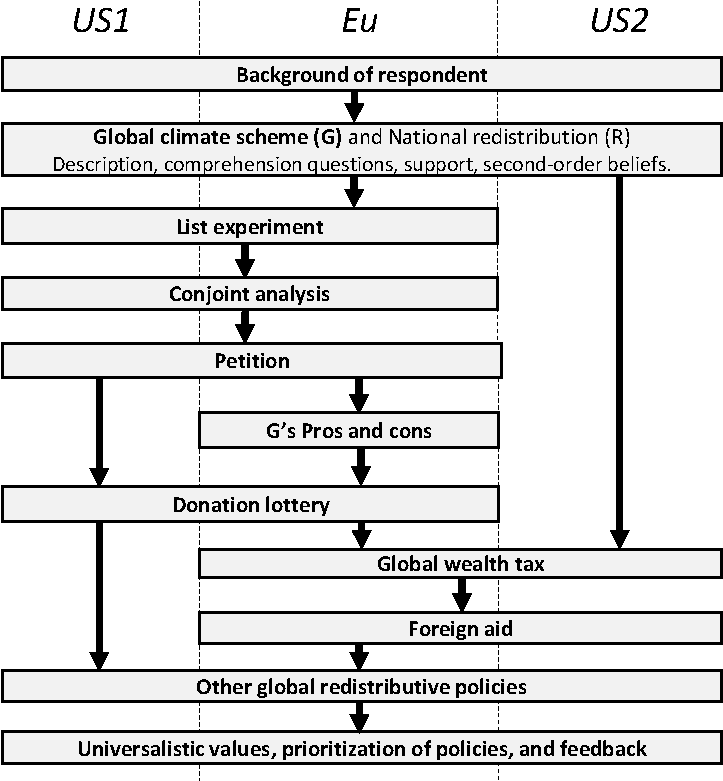
\includegraphics[width=.58\textwidth]{../questionnaire/survey_flow-simple.pdf}} 
\end{figure}

\begin{figure}[h!]
    % MAJOR figure
    \cprotect\caption[Relative support for global climate policies]{Relative Support for global climate policies\\ (\verb|OECD/Heatplot_global_tax_attitudes_share|).} 
    \makebox[\textwidth][c]{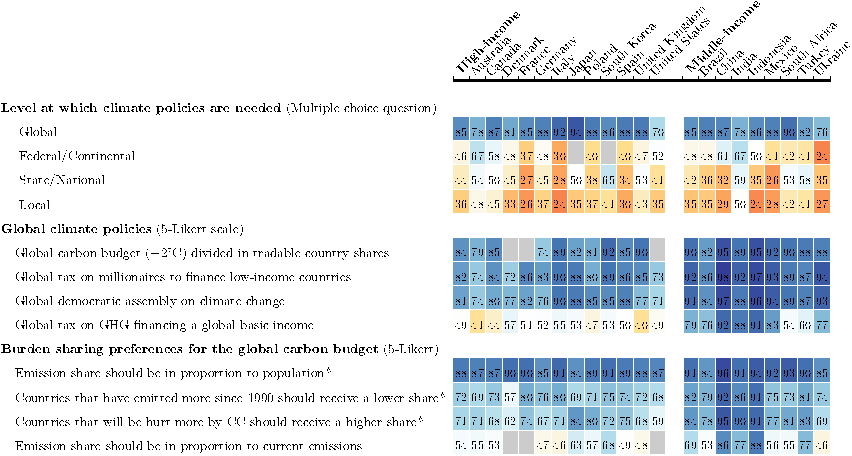
\includegraphics[width=1.2\textwidth]
    {../figures/OECD/Heatplot_global_tax_attitudes_share.pdf}}\label{fig:oecd} % with dependence on others (absent from OECD): Heatplot_burden_share_all_share_countries
    {\footnotesize \\ $\quad$ \\ Note 1: The numbers represent \textit{relative} support, i.e. the share of \textit{Somewhat} or \textit{Strongly support} among non-\textit{indifferent} answers (in percent, $n$ = 40,680). Shares of indifferent answers range from 11\% to 48\%, with quartiles 20\%, 27\%, and 33\%. The color blue denotes a relative majority. See Figure \ref{fig:oecd_absolute} for the absolute support. (Questions \ref{q:scale}-\ref{q:millionaire_tax}% Reproduced from \citealp{dechezlepretre_fighting_nodate}, Figure A21.
  ). \\ Note 2: *In Denmark, France and the U.S., the questions with an asterisk were asked differently, cf. Question \ref{q:burden_sharing_asterisk}. } 
\end{figure}


\begin{table}[h]
  % MAJOR figure % TODO! same table for NR in appendix
  % TODO table by country
  \caption[List experiment: tacit support for the GCS]{Number of supported policies in the list experiment depending on the presence of the Global Climate Scheme (GCS) in the list. %in function of the composition of the list. GCS stands for the Global Climate Scheme and NR for the National Redistribution Scheme.} % Beware, this question is quite unusual. \\ Among the policies below, how many do you support?  \\ Coal exit, Marriage only for opposite-sex couples 
   The tacit support for the GCS is estimated by regressing the number of supported policies on the presence of the GCS in the list of policies. The social desirability is estimated as the difference between the tacit and stated support (see Methods), and it is not significantly different from zero even at a 20\% threshold (as shown by the 80\% Confidence Interval).
  }\label{tab:list_exp}
  \makebox[\textwidth][c]{
\begin{tabular}{@{\extracolsep{5pt}}lccc} 
\\[-1.8ex]\hline 
\hline \\[-1.8ex] 
 & \multicolumn{3}{c}{Number of supported policies} \\ 
\cline{2-4} 
\\[-1.8ex] & All & US & Europe \\ 
\hline \\[-1.8ex] 
 List contains: GCS & 0.624$^{***}$ & 0.524$^{***}$ & 0.724$^{***}$ \\ 
  & (0.028) & (0.041) & (0.036) \\ 
\hline  \\[-1.8ex] \textit{Support for GCS} & 0.65  &  0.542  &  0.757 \\
\textit{Social desirability bias} & \textit{$ -0.026 $} & \textit{$ -0.018 $} & \textit{$ -0.033 $}\\
\textit{80\% C.I. for the bias} & \textit{ $[ -0.06 ; 0.01 ]$ } & \textit{ $[ -0.07 ; 0.01 ]$} & \textit{ $[ -0.08 ; 0.01 ]$}\\
 \hline \\[-1.8ex] 
Constant & 1.317 & 1.147 & 1.486 \\ 
Observations & 6,000 & 3,000 & 3,000 \\ 
R$^{2}$ & 0.089 & 0.065 & 0.125 \\ 
\hline 
\hline \\[-1.8ex] 
\textit{Note:}  & \multicolumn{3}{r}{$^{*}$p$<$0.1; $^{**}$p$<$0.05; $^{***}$p$<$0.01} \\ 
\end{tabular} 
  }  
  % {\footnotesize \textit{Note:} $^{*}p<0.1$; $^{**} p<0.05$; $^{***} p<0.01$.}
\end{table}

\begin{table}[h]
  % MAJOR figure
  \cprotect\caption[Influence of the GCS on electoral prospects]{Preference for a progressive platform depending on whether it includes the GCS or not. (Question \ref{q:conjoint_c}) 
  %Imagine if the [Democratic and Republican presidential candidates in 2024] campaigned with the following policies in their platforms. [Credible Progressive and Conservative platforms] \\ % TODO See More
% Which of these candidates would you vote for? \textit{A; B; None of them} \\
% ~[FR: second round of presidential; DE, ES, UK: two favorite candidates in one's constituency]
} % Beware, this question is quite unusual. \\ Among the policies below, how many do you support?  \\ Coal exit, Marriage only for opposite-sex couples 
  \makebox[\textwidth][c]{
\begin{tabular}{@{\extracolsep{5pt}}lcccccc} 
\\[-1.8ex]\hline 
\hline \\[-1.8ex] 
 & \multicolumn{6}{c}{Prefers the Progressive platform} \\ 
\cline{2-7} 
\\[-1.8ex] & All & United States & France & Germany & UK & Spain \\ 
\hline \\[-1.8ex] 
 GCS in Progressive platform & 0.028 & 0.029 & 0.112 & 0.015 & 0.008 & $-$0.015 \\ 
 95\% C.I. & ($-$.00, .06) & ($-$.01, .07) & (.03, .19) & ($-$.05, .08) & ($-$.07, .09) & ($-$.09, .06) \\ 
 P-value & 0.057 & 0.185 & 0.007 & 0.647 & 0.844 & 0.698 \\ 
 t & 1.904 & 1.326 & 2.730 & 0.458 & 0.197 & $-$0.388 \\ 
 \hline \\[-1.8ex] 
Constant & 0.623 & 0.604 & 0.55 & 0.7 & 0.551 & 0.775 \\ 
Observations & 5,202 & 2,619 & 605 & 813 & 661 & 504 \\ 
R$^{2}$ & 0.001 & 0.001 & 0.013 & 0.0003 & 0.0001 & 0.0003 \\ 
\hline 
\hline \\[-1.8ex] 
\end{tabular} }\label{tab:conjoint_c}
  {\footnotesize \textit{Note:} Simple OLS model with robust standard errors (HC1). %P-values are reported in parentheses. 
  The 14\% of \textit{None of them} answers have been excluded from the regression samples. GCS has no significant influence on them. $^{*}p<0.1$; $^{**} p<0.05$; $^{***} p<0.01$. 
  }
\end{table}

\begin{figure}[h!]
    % MAJOR figure
    \cprotect\caption[Relative support for other global policies]{Relative support for various global policies. (percentage of \textit{somewhat} or \textit{strong support}, after excluding \textit{indifferent} answers; *except for GCS: percentage of \textit{Yes} in a \textit{Yes}/\textit{No} question, preferred share: percentage of answers $\geq$30\%, and foreign aid: percentage of unconditional or conditional increase rather than decrease or stable aid). Shares of indifferent answers range from 10\% to 40\%, with quartiles 19\%, 25\%, and 32\%. (\verb|support_likert_all_share|; p. \pageref{subsec:questionnaire_GCS}, Questions \ref{q:gcs_support}, \ref{q:global_tax_global_share}, \ref{q:climate_policies}, \ref{q:other_policies}, and \ref{q:foreign_aid_raise_support}; See Figure \ref{fig:support_likert_positive} for the absolute support.)% $n_\text{US} = n_\text{Eu} = 3,000,\, n_\text{FR} = 729,\, n_\text{DE} = 929,\, n_\text{ES} = 543,\, n_\text{UK} = 749, n_\text{US, global/national wealth tax} = 2,000$
    }
    \makebox[\textwidth][c]{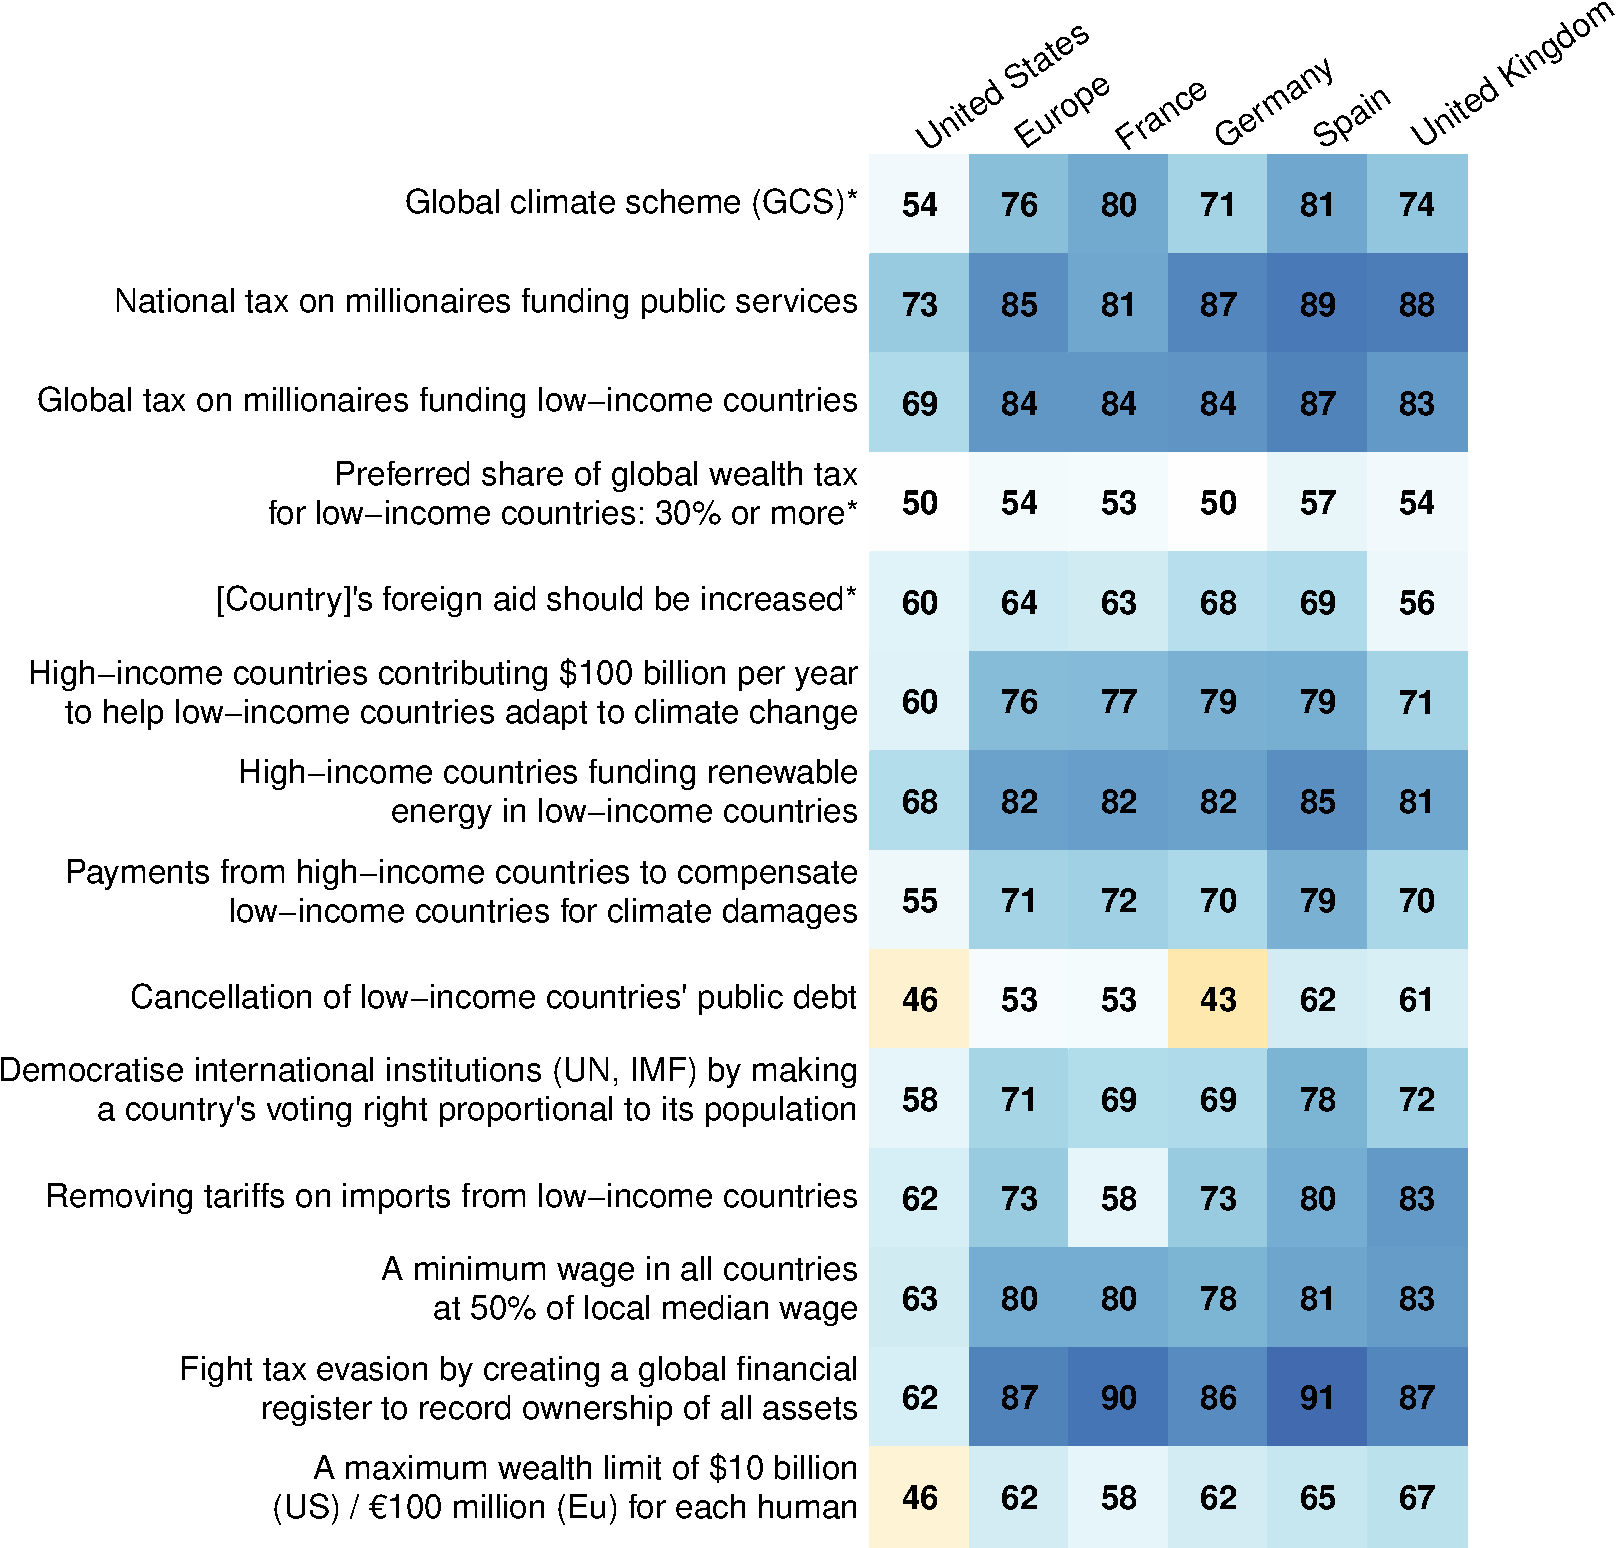
\includegraphics[width=\textwidth]{../figures/country_comparison/support_likert_all_share.pdf}}\label{fig:support}
\end{figure} 

\renewcommand{\thetable}{ED\arabic{table}}
\renewcommand{\thefigure}{ED\arabic{figure}}
\setcounter{figure}{0}
\setcounter{table}{0}


\begin{table}[h]
    \cprotect\caption[Campaign and bandwagon effects on the support for the GCS.]{Effects on the support for the GCS of a question on its pros and cons (either in open-ended of closed format) and on information about the actual support, in the U.S. (See Section \ref{subsec:questionnaire_perceptions} in the \textit{US2} Questionnaire)  %\hfill (Back~to~Section~\ref{subsubsec:pros_cons})
    } \label{tab:branch_gcs}
    \makebox[\textwidth][c]{
        
\begin{tabular}{@{\extracolsep{5pt}}lcccc} 
\\[-1.8ex]\hline 
\hline \\[-1.8ex] 
 & \multicolumn{4}{c}{Support} \\ 
\cline{2-5} 
\\[-1.8ex] & \multicolumn{2}{c}{Global Climate Scheme} & \multicolumn{2}{c}{National Redistribution} \\ 
\\[-1.8ex] & (1) & (2) & (3) & (4)\\ 
\hline \\[-1.8ex] 
Control group mean & 0.557 & 0.557 & 0.569 & 0.569  \\ \hline \\[-1.8ex]
 Treatment: Open\mbox{-}ended field on GCS pros \& cons & $-$0.073 & $-$0.073 & $-$0.035 & $-$0.031 \\ 
  & ($-$.14, $-$.01) & ($-$.13, $-$.01) & ($-$.10, .03) & ($-$.09, .03) \\ 
  & p = 0.035 & p = 0.020 & p = 0.310 & p = 0.337 \\ 
  Treatment: Closed questions on GCS pros \& cons & $-$0.109 & $-$0.096 & $-$0.065 & $-$0.062 \\ 
  & ($-$.18, $-$.04) & ($-$.16, $-$.04) & ($-$.13, .00) & ($-$.12, $-$.00) \\ 
  & p = 0.002 & p = 0.002 & p = 0.056 & p = 0.046 \\ 
  Treatment: Info on actual support for GCS and NR & $-$0.021 & $-$0.017 & 0.048 & 0.054 \\ 
  & ($-$.09, .05) & ($-$.08, .04) & ($-$.02, .11) & ($-$0.01, 0.11) \\ 
  & p = 0.536 & p = 0.586 & p = 0.145 & p = 0.084 \\ 
 \hline \\[-1.8ex] 
Includes controls &  & \checkmark &  & \checkmark \\

Observations & 2,000 & 1,995 & 2,000 & 1,995 \\ 
R$^{2}$ & 0.007 & 0.169 & 0.007 & 0.153 \\ 
\hline 
\hline \\[-1.8ex] 
\end{tabular} 
    }
    {\footnotesize %\textit{Note}: 
    }
  \end{table}
  
  \begin{table}[h]
    \cprotect\caption[Donation to Africa vs. own country]{Donation in case of lottery win, depending on the recipient's (randomly drawn) nationality. (Question \ref{q:donation})%\hfill (Back~to~Section~\ref{subsec:universalistic})
    } \label{tab:donation}
    \makebox[\textwidth][c]{
\begin{tabular}{@{\extracolsep{5pt}}lcccc} 
\\[-1.8ex]\hline 
\hline \\[-1.8ex] 
 & \multicolumn{4}{c}{Donation to poor people (in \%)} \\ 
\cline{2-5} 
\\[-1.8ex] & All & US & US & Eu \\ 
\hline \\[-1.8ex] 
 Poor is in own country & 0.590 & 2.509 & 0.046 & $-$1.349 \\ 
  & ($-$0.977, 2.156) & (0.252, 4.766) & ($-$3.268, 3.361) & ($-$3.521, 0.823) \\ 
  & p = 0.461 & p = 0.030 & p = 0.979 & p = 0.224 \\ 
  Poor is in own country $\times$ Vote: \textit{not} Biden &  &  & 3.954 &  \\ 
  &  &  & ($-$0.512, 8.420) &  \\ 
  &  &  & p = 0.083 &  \\ 
 \hline \\[-1.8ex] 
Mean & 34.034 & 33.658 & 33.658 & 34.41 \\ 
Observations & 6,000 & 3,000 & 3,000 & 3,000 \\ 
R$^{2}$ & 0.0001 & 0.002 & 0.034 & 0.0005 \\ 
\hline 
\hline \\[-1.8ex] 
\end{tabular} }
  \end{table}
  
  \begin{table}[h]

\caption{\label{tab:amce}Average Marginal Component Effects of global policies.}
\makebox[\textwidth][c]{
\begin{tabular}[t]{lccccc}
\toprule
  & Effect & Obs. & t & P-value & 95\% C.I.\\
\midrule
FR; Global Climate Plan & 0.13*** & 1456 & 3.5 & $5\cdot 10^{-4}$ & {}[0.06; 0.21]\\
DE; Global Climate Plan & 0.09** & 1958 & 2.8 & 0.005 & {}[0.03; 0.16]\\
ES; Global Climate Plan & 0.04 & 1086 & 0.82 & 0.411 & {}[-0.05; 0.12]\\
UK; Global Climate Plan & 0.09* & 1498 & 2.31 & 0.021 & {}[0.01; 0.16]\\
US; Global Climate Plan & 0.01 & 4436 & 0.61 & 0.539 & {}[-0.03; 0.06]\\
FR; Global Millionaire Tax & 0.11* & 1456 & 2.49 & 0.013 & {}[0.02; 0.2]\\
DE; Global Millionaire Tax & 0.09* & 1958 & 2.3 & 0.022 & {}[0.01; 0.18]\\
ES; Global Millionaire Tax & 0.05 & 1086 & 0.91 & 0.365 & {}[-0.06; 0.16]\\
UK; Global Millionaire Tax & 0.13** & 1498 & 2.86 & 0.004 & {}[0.04; 0.22]\\
US; Global Millionaire Tax & 0.09** & 4436 & 3.16 & 0.002 & {}[0.03; 0.14]\\
FR; Global Democratic Assembly on Climate Change & 0.12* & 1456 & 2.52 & 0.012 & {}[0.03; 0.21]\\
DE; Global Democratic Assembly on Climate Change & 0.1* & 1958 & 2.52 & 0.012 & {}[0.02; 0.18]\\
ES; Global Democratic Assembly on Climate Change & -0.01 & 1086 & -0.22 & 0.829 & {}[-0.12; 0.1]\\
UK; Global Democratic Assembly on Climate Change & 0.07 & 1498 & 1.56 & 0.12 & {}[-0.02; 0.17]\\
US; Global Democratic Assembly on Climate Change & 0.08** & 4436 & 2.93 & 0.003 & {}[0.03; 0.13]\\
\bottomrule
\end{tabular}}
\end{table}
  
  % \begin{figure}[h!]
  %     \cprotect\caption[Support for the Global Climate Scheme]{[For Supplementary Material] Support for the GCS, NR and the combination of GCS, NR and C (\textit{Yes}/\textit{No} questions). \\(p. \pageref{subsec:questionnaire_GCS}, Questions \ref{q:gcs_support}, \ref{q:nr_support}, \ref{q:global_tax}, \ref{q:national_tax}, and \ref{q:crg_support}).%; $n_\text{US} = n_\text{Eu} = 3,000,\, n_\text{FR} = 729,\, n_\text{DE} = 929,\, n_\text{ES} = 543,\, n_\text{UK} = 749$)
  %     }\label{fig:support_binary}
  %     \makebox[\textwidth][c]{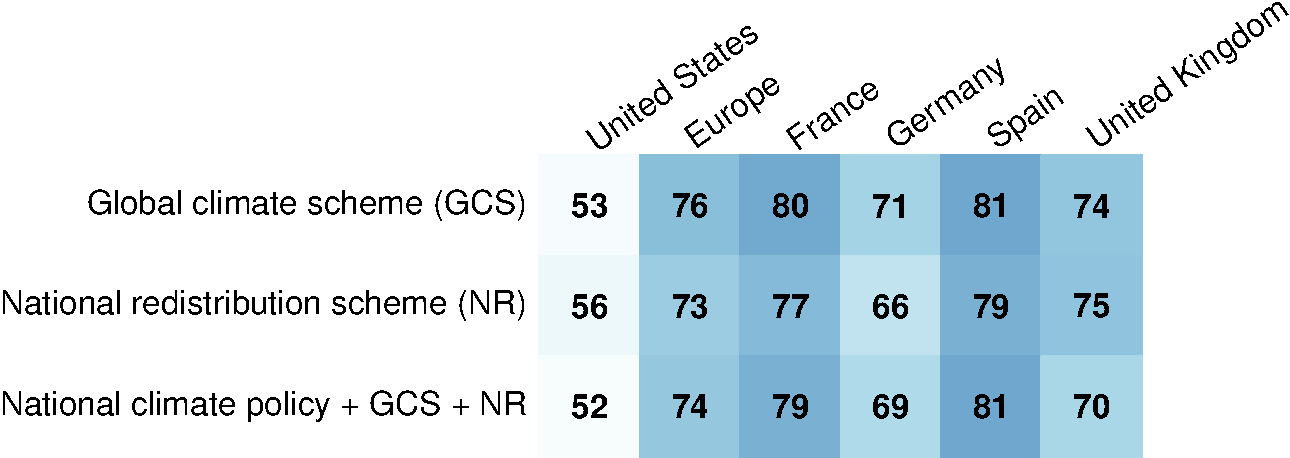
\includegraphics[width=.9\textwidth]{../figures/country_comparison/support_binary_positive.pdf}} 
  % \end{figure}
  
  % TODO?: add note to the figure above, to explain what is the national climate policy.
   
  \begin{figure}[h] 
    \cprotect\caption[Preferences for various policies in political platforms]{Effects of the presence of a policy (rather than none from this domain) in a random platform on the likelihood that it is preferred to another random platform. (See non-translated versions in Figure \ref{fig:ca_r_en}; \verb|[country]/ca_r|; Question \ref{q:conjoint_r}%; in the U.S., asked only to non-Republicans.
    )}\label{fig:ca_r}
    \begin{subfigure}{\textwidth}
      \subcaption{U.S. (Asked only to non-Republicans)}
      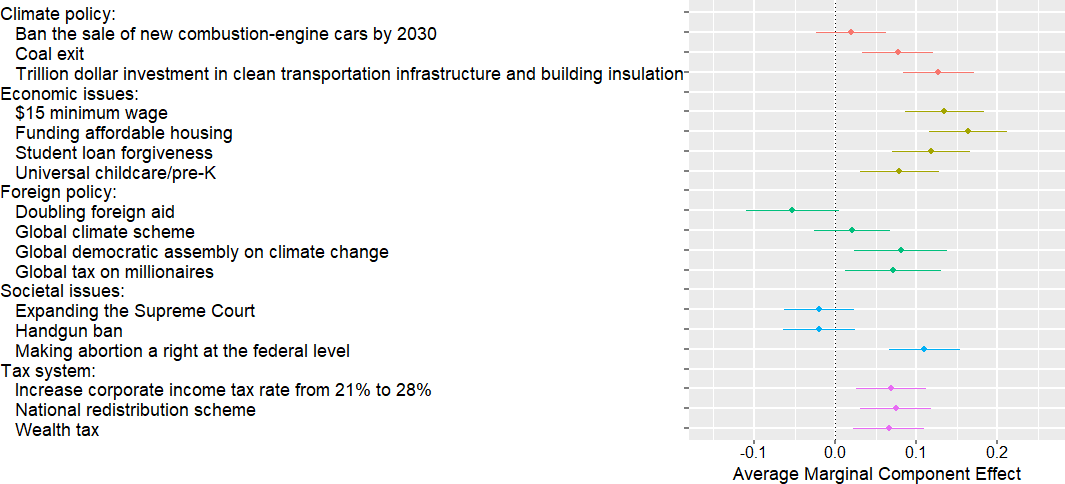
\includegraphics[width=\textwidth]{../figures/US1/ca_r.png}
    \end{subfigure}
    \begin{subfigure}{\textwidth}
      \subcaption{France}
      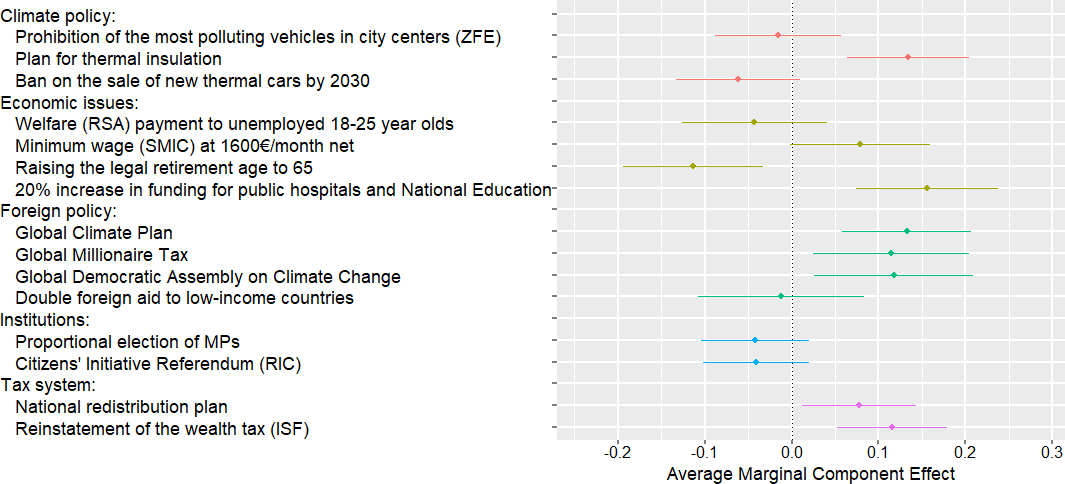
\includegraphics[width=\textwidth]{../figures/FR/ca_r_en.png}
    \end{subfigure}
  \end{figure}%
  \clearpage
  \begin{figure}[h!]\ContinuedFloat % if bugs try b! instead of h!
    \begin{subfigure}{\textwidth}
      \subcaption{Germany}
      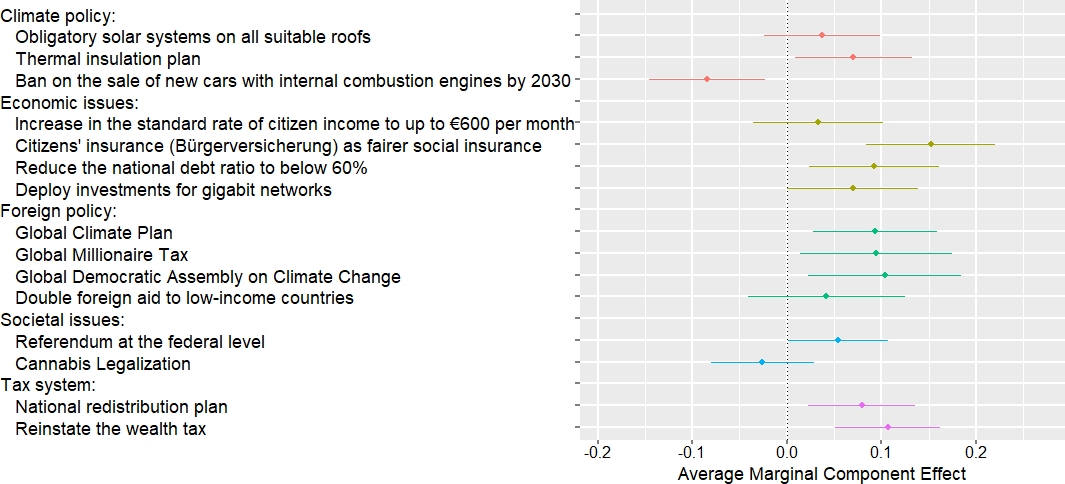
\includegraphics[width=\textwidth]{../figures/DE/ca_r_en.png}
    \end{subfigure}
    \begin{subfigure}{\textwidth}
      \subcaption{Spain}
      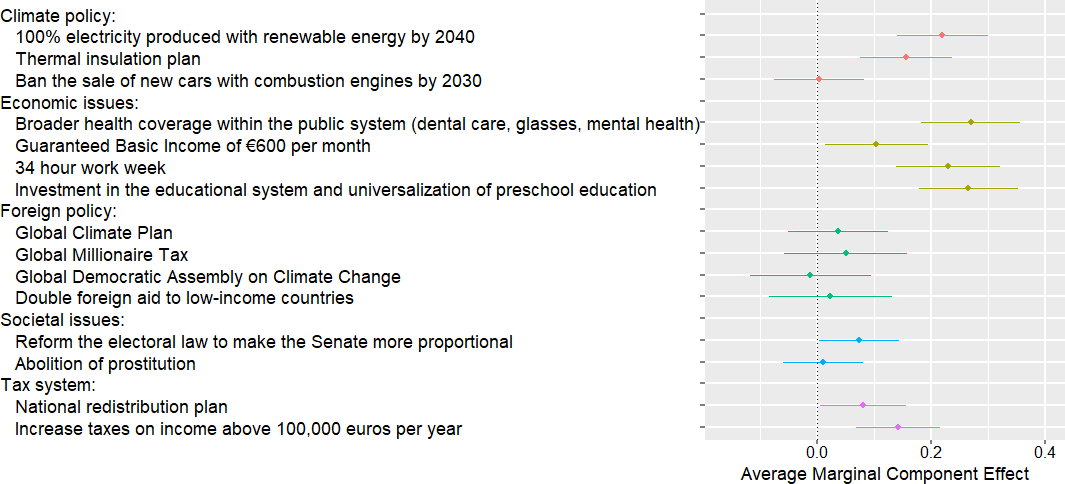
\includegraphics[width=\textwidth]{../figures/ES/ca_r_en.png}
    \end{subfigure}
    \begin{subfigure}{\textwidth}
      \subcaption{UK}
      \includegraphics[width=\textwidth]{../figures/UK/ca_r.png}
    \end{subfigure}
    %\makebox[\textwidth][c]{} 
  \end{figure}
  
  \begin{figure}[h!]
    \cprotect\caption[Influence of the GCS on preferred platform]{Influence of the GCS on preferred platform:\\ Preference for a random platform A that contains the Global Climate Scheme rather than a platform B that does not (in percent). (\verb|conjoint_left_ag_b_binary_positive|; Question \ref{q:conjoint_d}; in the U.S., asked only to non-Republicans.)}\label{fig:conjoint_left_ag_b}
    \makebox[\textwidth][c]{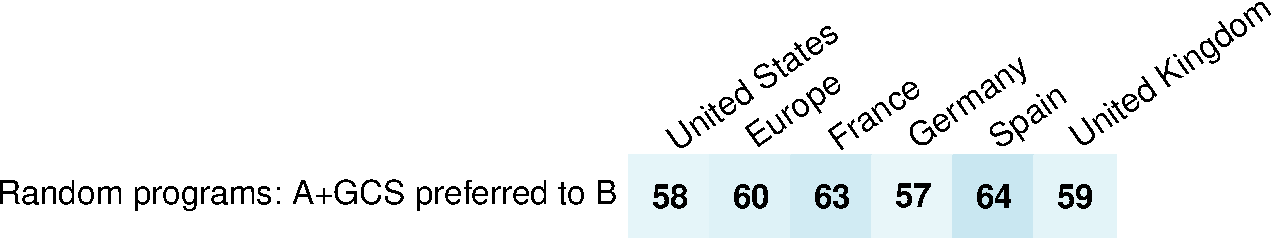
\includegraphics[width=\textwidth]{../figures/country_comparison/conjoint_left_ag_b_binary_positive.pdf}} 
  \end{figure}
  
  \begin{figure}[h!]
    \cprotect\caption[Beliefs about support for the GCS and NR]{Beliefs regarding the support for the GCS and NR. (\verb|belief_all_mean|; Questions \ref{q:gcs_belief} and \ref{q:nr_belief})}\label{fig:belief}
    \makebox[\textwidth][c]{
\includegraphics[width=.7\textwidth]{../figures/country_comparison/belief_all_mean.pdf}} 
  \end{figure}
  
  \begin{figure}
    \centering 
    \cprotect\caption[Preferred share of wealth tax for low-income countries]{Percent of global wealth tax that should finance low-income countries (\textit{mean}). \\ ``Imagine a wealth tax on households with net worth above [\$]5 million, enacted in all countries around the world.  
    (\dots)  \\
    What percentage should be pooled to finance low-income countries (instead of retained in the country's national budget)?'' (\verb|global_tax_global_share_mean|; Question \ref{q:global_tax_global_share})} % TODO? n
    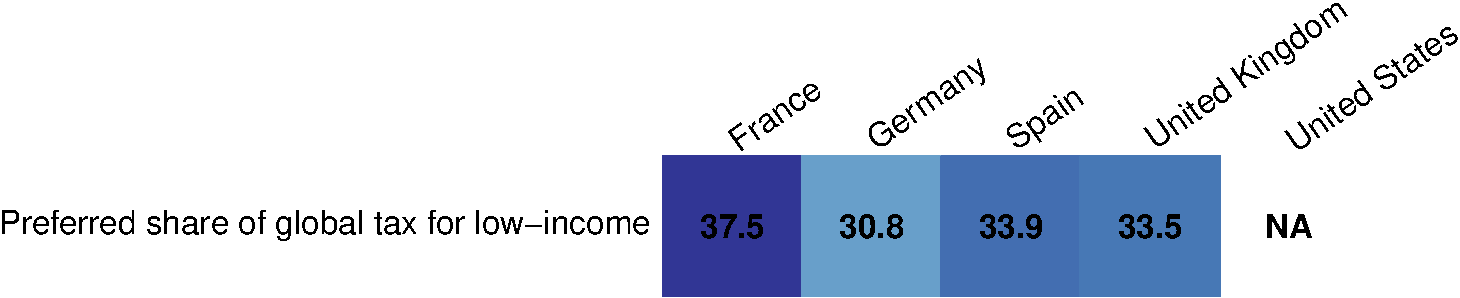
\includegraphics[width=1\textwidth]{../figures/country_comparison/global_tax_global_share_mean.pdf} \label{fig:global_share_mean}
  \end{figure}
  
  \begin{figure}[h!]
    \cprotect\caption[Attitudes on the evolution of foreign aid]{Attitudes regarding the evolution of [own country] foreign aid. (\verb|foreign_aid_raise_support|; Question \ref{q:foreign_aid_raise_support})}\label{fig:foreign_aid_raise_support}
    \makebox[\textwidth][c]{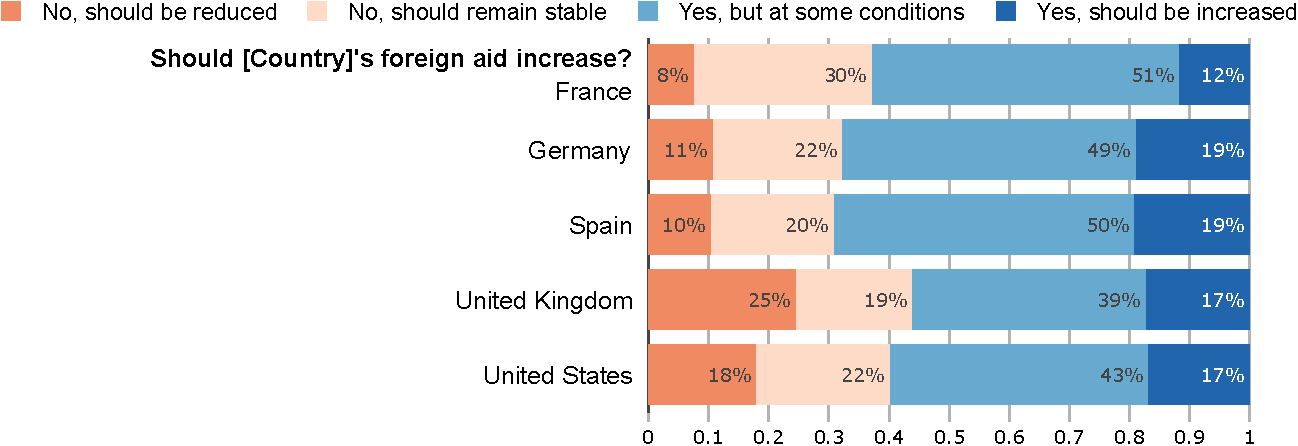
\includegraphics[width=\textwidth]{../figures/country_comparison/foreign_aid_raise_support.pdf}} 
  \end{figure}
  
  \begin{figure}[h!]
    \cprotect\caption[Conditions at which foreign aid should be increased]{Conditions at which foreign aid should be increased (in percent). [Asked to those who wish an increase of foreign aid at some conditions.] (\verb|foreign_aid_condition_positive|; Question \ref{q:foreign_aid_condition})}\label{fig:foreign_aid_condition}
    \makebox[\textwidth][c]{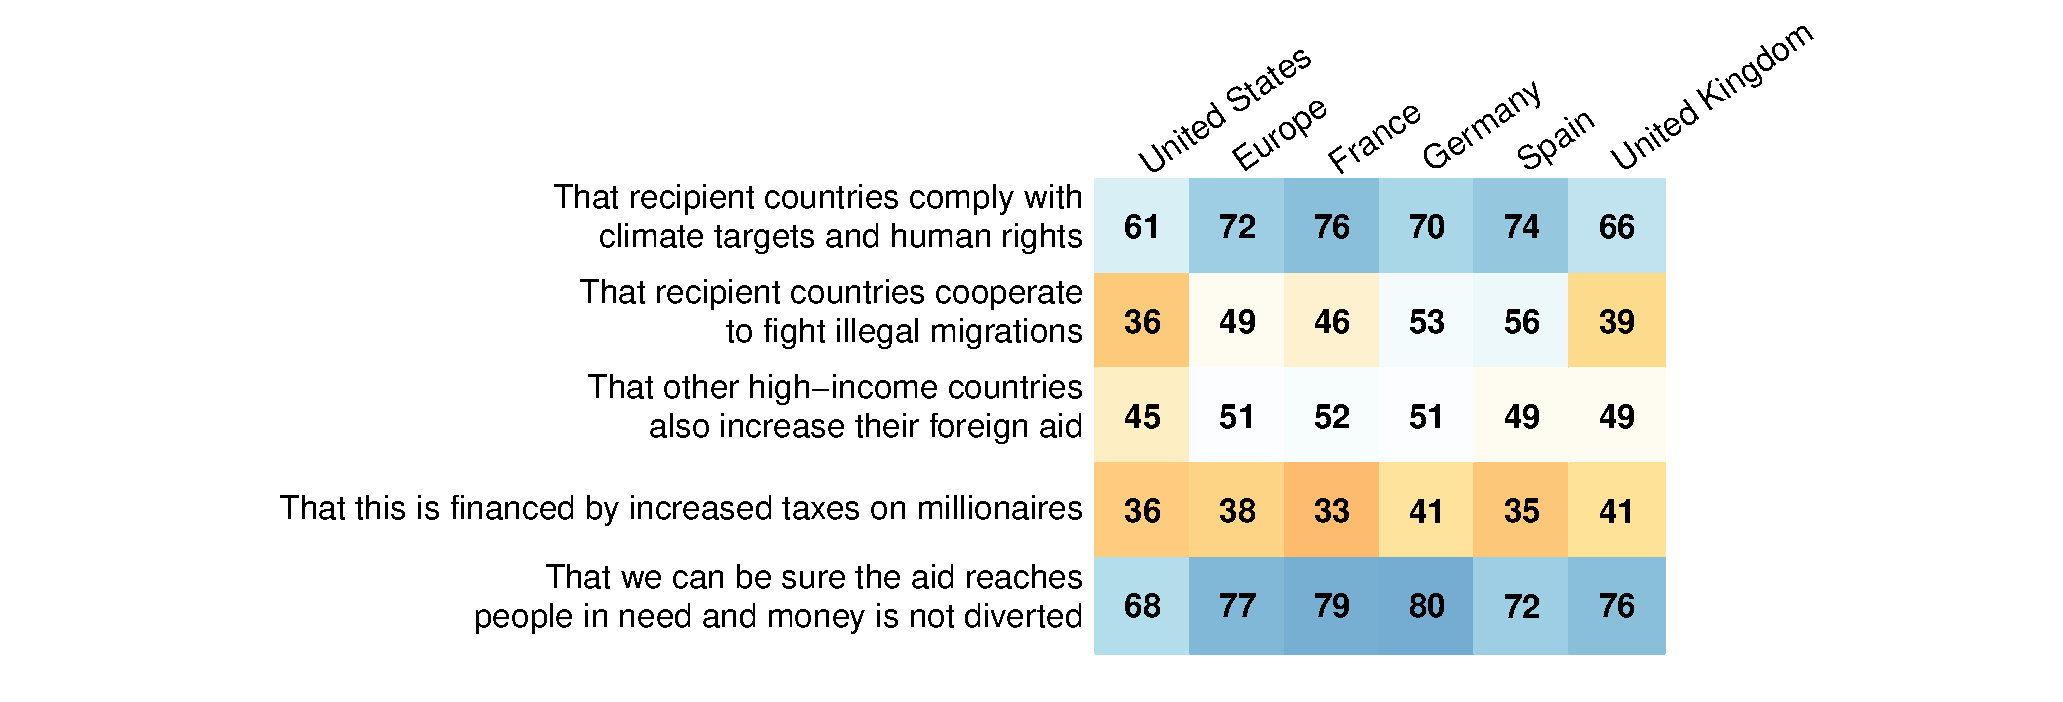
\includegraphics[width=\textwidth]{../figures/country_comparison/foreign_aid_condition_positive.pdf}} 
  \end{figure}
  
  \begin{figure}[h!]
    \cprotect\caption[Reasons why foreign aid should not be increased]{Reasons why foreign aid should not be increased (in percent). [Asked to those who wish a decrease or stability of foreign aid.] (\verb|foreign_aid_no_positive|; Question \ref{q:foreign_aid_no})}\label{fig:foreign_aid_no}
    \makebox[\textwidth][c]{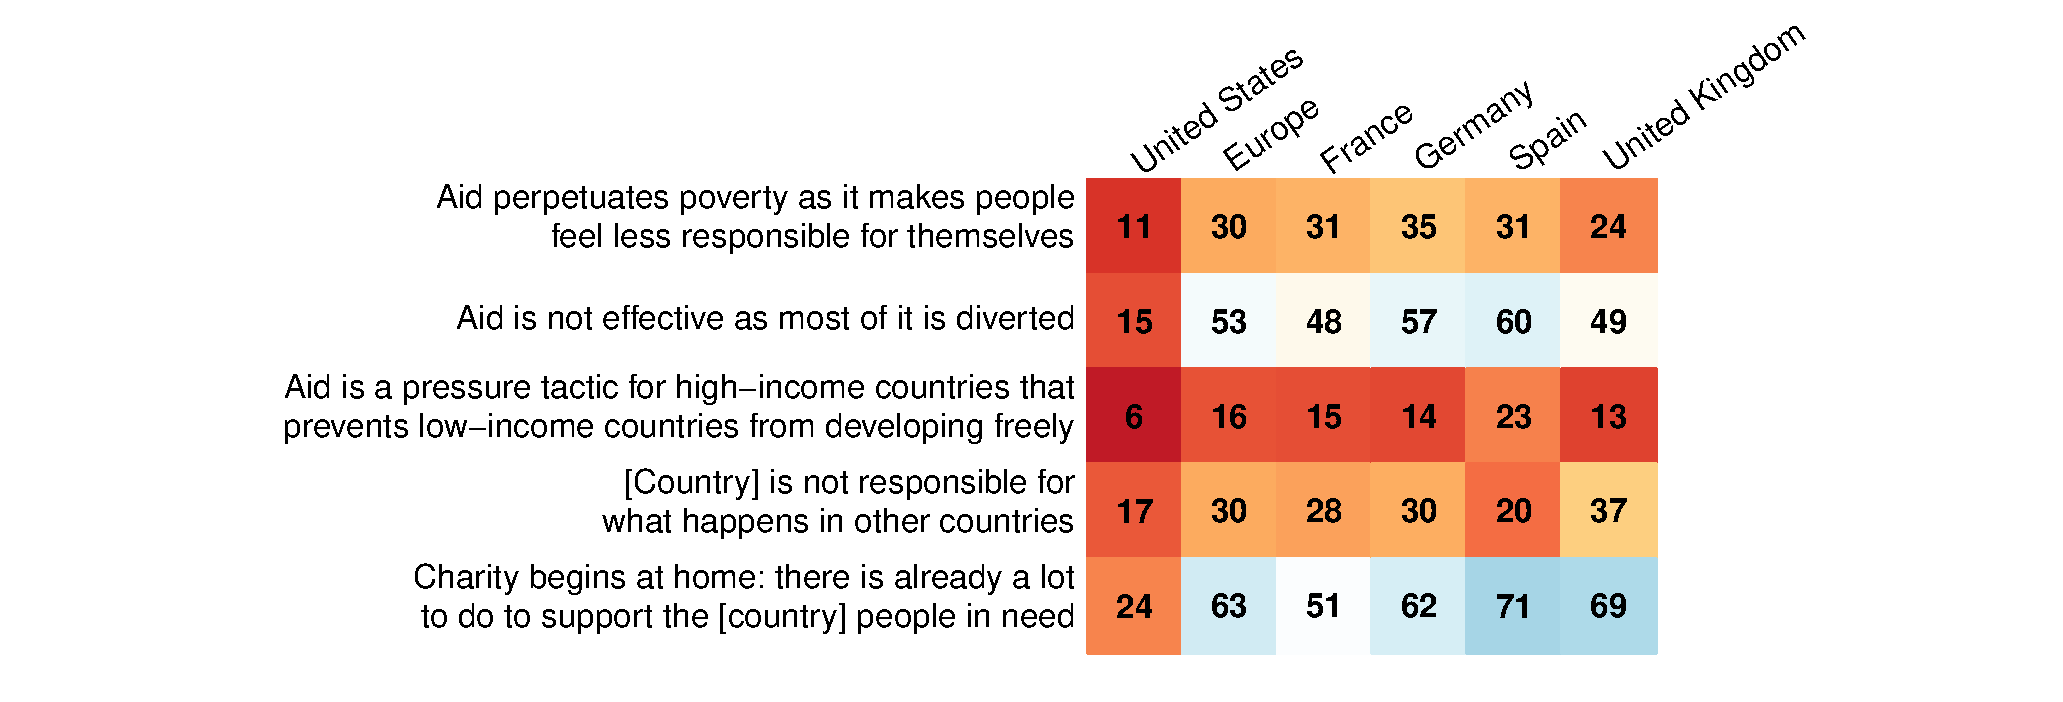
\includegraphics[width=\textwidth]{../figures/country_comparison/foreign_aid_no_positive.pdf}} 
  \end{figure}

\appendix 
\renewcommand{\thetable}{S\arabic{table}}
\renewcommand{\thefigure}{S\arabic{figure}}
\setcounter{figure}{0}
\setcounter{table}{0}

% TODO! Ipsos (2023)
% TODO! list experiment, world citizenship, elite surveys, etc.
% TODO Norway and foreign aid
% TODO Cite Leiserowitz (06)
% TODO? Cite Whitmarsh & Capstick?
\clearpage
\section{Literature review}\label{sec:literature}

\subsection{Attitudes and perceptions}\label{subsec:literature_attitudes}

\subsubsection{Population attitudes on global policies}\label{subsubsec:literature_attitudes_policies}
% Our surveys fill gaps in the knowledge of attitudes toward global policies. 
% We are not aware of any other survey on a global wealth tax. 
Using representative samples in 125 countries covering 96\% of the world's greenhouse gas emissions, \citeRt{andre_globally_2024} show that 69\% of the global population express willingness to contribute 1\% of their income to fight global warming.\footnote{However, \citeRt{ipsos_earth_2023} find no majority support when the amount is not specified, despite strong agreement for own individual action.} 
\citeRt{carattini_how_2019} test the support for six variants of a global carbon tax on samples in five countries, representative along gender and age. For a given variant, the sample size is about 167 respondents per country. They find over 80\% support for any variant in India, between 50\% and 65\% in Australia, the UK and South Africa, and 43\% to 59\% in the U.S., depending on the variant. Notably, the support for a global carbon tax funding an equal dividend for each human is close to 50\% in high-income countries (e.g., at 44\% in the U.S.), consistently with our results from the \textit{Global} survey (see Figure \ref{fig:oecd}). This is another piece of evidence that the support is lower for a tax that would ``only'' reduce CO$_\text{2}$ emissions than for a quota that would unambiguously achieve the climate target. %Given that \citeRt{carattini_how_2019} do not explain that the policy would reduce extreme poverty and test a \textit{tax} that would only reduce CO$_\text{2}$ emissions (rather than achieve the climate target), the support is consistent with the support for a tax observed in the global survey (see Figure \ref{fig:oecd}), and somewhat lower than what the support for the GCS. 
In a survey over 15 countries, \citeRt{bloodworth_money_2023} find 73\% agreement to tax fossil fuel companies and finance climate action in poorer countries. 
Using a conjoint analysis in the U.S. and Germany, \citeRt{beiser-mcgrath_could_2019} find that the support for a carbon tax increases by up to 50\% % e.g. in their Fig. 4 the DE support for $70/t jumps from 26 to 39% with extension to all industrialized countries
if it applies to all industrialized countries rather than exclusively to one's own country. % Variant of carbon tax is 8 (US) - 17 (DE) p.p. more likely to be preferred if tax is extended to all industrialized countries

In surveys conducted in Brazil, Germany, Japan, the UK and the U.S., \citeRt{ghassim_who_2020} finds support ranging from 55\% to 74\% for ``a global democracy including both a global government and a global parliament, directly elected by the world population, to recommend and implement policies on global issues''. \citeRt{ghassim_who_2024} also finds strong support for a democratic world government in surveys over 17 countries. % (for example, international peace, world poverty, and climate change)''
Furthermore, through an experiment, \citeRt{ghassim_who_2020} finds that, in countries where the government stems from a coalition, voting shares would shift by 8 (Brazil) to 12 p.p. (Germany) from parties who are said to oppose global democracy to parties that supposedly support it. For instance, when Germans respondents were told that (only) the Greens and the Left support global democracy, these parties gained respectively 9 and 3 p.p. in vote intentions, while the SPD and the CDU-CSU each lost 6 p.p. 
\citeRt{ghassim_who_2020} also presents survey results showing strong majorities in favor of the direct election of one's country's UN representative in all 18 surveyed countries. % same as unpa_survey_2005 % GlobeScan 2005; also: half/half (majorities or not depend on the country) for “Global Parliament, where votes are based on country population sizes, and the global parliament is able to make binding policies” (Synovate 2007); also: (GlobeScan 22, not from Ghassim) in 31 countries: 77% agree that “Rich countries must pay for poorer countries do deal with the effects of CC” 
Similarly, in each of 10 countries, there are clear majorities in favor of ``a new supranational entity [taking] enforceable global decisions in order to solve global risks'' \citeRp{global_challenges_foundation_attitudes_2018}. Remarkably, already in 1946, 54\% of Americans agreed (while 24\% disagreed) that ``the UN should be strengthened to make it a world government with the power to control the armed forces of all nations'' \citeRp{gallup_seventy_1946}. 
Furthermore, in surveys conducted in Argentina, China, India, Russia, Spain, and the U.S., \citeRt{ghassim_public_2022} find majority support for UN reforms that would make United Nations' decisions binding, give veto powers to a few other major countries at the Security Council, or complement the highest body of the UN with a chamber of directly elected representatives. 

Relatedly, \citeRt{meilland_international_2024} find that both Americans and French people prefer an international settlement of climate justice, even if it encroaches on sovereignty. In a 2013 survey conducted in China, Germany, and the U.S., \citeRt{schleich_citizens_2016} show that over three-quarter of people think that international climate agreements reached so far are not successful and that future agreements are important. % 73\% of people find important future international climate agreements, while less than 26\% think that international reached so far are successful. 
In Finland, \citeRt{sivonen_attitudes_2022} finds that that support for a carbon tax is higher if implemented at the global level (54\%) rather than at the national level (40\%).

The results from these specific questions are in line with the answers to more general questions. In each of 36 countries, \citeRt{issp_international_2010} find near consensus that ``for environmental problems, there should be international agreements that [their country] and other countries should be made to follow'' (overall, 82\% agree and 4\% disagree). % No question like this in the next Envi wave in 2022
In each of 29 countries, \citeRt{issp_international_2019} uncover near consensus that ``Present economic differences between rich and poor countries are too large'' (overall, 78\% agree and 5\% disagree). \citeR{leiserowitz_public_2021} reveal that 66\% of Americans support providing ``financial aid and technical support to developing countries that agree to limit their greenhouse gas emissions.'' \citeRt{fehr_your_2022} find that 90\% of Germans want some degree of global redistribution. %support for global and national redistribution are correlated.
%* Also in ISSP (19): slight minorities (in rich countries) that “People in wealthy countries should make an additional tax contribution to help people in poor countries.” p. 104, but strong majorities everywhere that “People from poor countries should be allowed to work in wealthy countries.” p. 106

%* ISSP (19): Near consensus that “Present economic differences between rich and poor countries are too large.” p. 102, slight minorities (in rich countries) that “People in wealthy countries should make an additional tax contribution to help people in poor countries.” p. 104, but strong majorities everywhere that “People from poor countries should be allowed to work in wealthy countries.” p. 106
%* Ghassim et al. (22): support for stronger UN with more direct elections.
%* Ghassim (20):  in Germany those two parties that supposedly endorse global democracy – the Greens and the Left – benefitted, gaining nine and three percentage points respectively in terms of voting intentions. Meanwhile, the traditional centrist parties – SPD and CDU – each lost six percentage points due to their supposed opposition to global democracy.
%* Beiser-McGrath & Bernauer (19): Conjoint analysis in US, DE. Variant of carbon tax is 8 (US) - 17 (DE) p.p. more likely to be preferred and 50% more likely to be supported if tax is extended to all industrialized countries (Fig 1, 4). (Unfortunately, don't test extension to global level).
%- Çarkoğlu.. (15) International Social Survey Program 2010 data reveal that people in LDCs are less supportive of international agreements forcing their country to take necessary environmental measures than are citizens in the developed world [80% instead of 85%]. (‘for environmental problems, there should be international agreements that [their country] and other countries should be made to follow.’)
%* Carattini et al. (Nature, 19): 1k in US, IA, ZA, AU, UK. Each respondent receives one variant at random of global carbon price of 40/60/80 $/t redistributed as international dividend / national dividend / mitigation in all countries / mitigation in developing countries / domestic mitigation / reduced labour tax. Immense majorities for any scheme in India, small majorities for each elsewhere except US international dividend (44%) or mitigation in developing (43%), and AU mitigation in developing (49,6%). PB: very low sample size (~167) for a given redistribution, even lower (~55) for a given variant (that also specifies the price). Appendix also contains estimation of distributive impacts. Representative only along the two quotas: gender and age. Don't give the representativeness in terms of income (the third socio-demos that they ask) so it's probably bad.

\subsubsection{Population attitudes on climate burden sharing}\label{subsubsec:literature_attitudes_burden_sharing}

Despite differences in the description of fairness principles, surveys on burden-sharing rules show consistent attitudes. Or at least, their seemingly contradictory results can be made compatible with the following interpretation: 
Concerning emissions reductions, most people want that every country engage in strong and collective decarbonization efforts, with a global quota converging to climate neutrality in the medium run. Concerning the financial effort, most people support high-emitting countries paying and low-income countries receiving funding. The most supported rules are those perceived as equitable, in particular an equal right to emit per person. 
% When the rankings between rules differ, it can be due to the difference in countries surveyed, but it is most often due to differences in definitions and wording. 

This interpretation helps to understand the apparent differences between articles that approach burden sharing from different angles: cost sharing (in money terms), effort sharing (in terms of emissions reductions), or resource sharing (in terms of rights to emit). Existing papers adopt either the cost sharing or effort sharing approach, which preclude any country from being a net receiver of funds. Also, by focusing on \textit{either} the financial or the decarbonization effort, these surveys miss the other half of the picture, which can explain why some papers find strong support for the ability-to-pay principle while others find strong support for grandfathering (defined as emissions reductions being the same in every country). The literature follows these approaches to align with the notions used by the UNFCCC. Yet, we argue that the resource sharing approach is preferable for uncovering attitudes, as it unambiguously describes the distributive implications of each rule while achieving an efficient geographical distribution of emissions reductions and explicitly allowing for monetary gains for some countries. % TODO? say more simply that the location of emissions reductions is flexible in resource sharing
% TODO? appendix with the definitions for each author, incl. us

Now, let us summarize the results of the different papers in the light of this clarification. 
\citeRt{schleich_citizens_2016} find an identical ranking of support for burden-sharing principles in China, Germany, and the U.S.: polluter-pays followed by ability-to-pay, equal emissions per capita, and grandfathering. 
% \footnote{The survey of \citeRt{schleich_citizens_2016} defines these rules as follows: \\
% \textit{Polluter-pays}: ``Every country has to bear costs according to the emissions it causes (hence countries causing higher emissions have a higher share of the costs).'' \\
% \textit{Ability-to-pay}: ``Every country has to bear costs according to its economic strength (hence richer countries have a higher share of the costs).''
% \textit{Egalitarianism}: ``Every country is allowed to produce the same amount of emissions per capita (hence countries with currently high emissions per capita have higher costs).''
% \textit{Sovereignty} (i.e. grandfathering): ``Every country is allowed to produce the same share of global emissions as in the past (hence the proportional reduction of emissions is the same for every country).''} 
Note that the authors do not allow for emissions trading in their description of equal \textit{emissions per capita}, which may explain its relatively low support. 
Yet, the relative support for egalitarianism also depends on how \textit{the other} rules are described. Indeed, \citeRt{carlsson_is_2011} find that Swedes prefer that ``all countries are allowed to emit an equal amount per capita'' rather than options where emissions are reduced based on current or historical emissions, for which it is explicitly stated that high-emitting countries ``will continue to emit more than others''. 
\citeRt{bechtel_mass_2013} find agreement that rich countries should pay more and historical emissions should matter, but that efforts should not be solely borne by wealthy nations. More precisely, their conjoint analysis conducted in France, Germany, the UK, and the U.S. shows that a climate agreement is 15 p.p. more likely to be preferred  (to a random alternative) if it includes 160 countries rather than 20, and 5 p.p. less likely to be preferred if ``only rich countries pay'' compared to other burden-sharing rules: ``rich countries pay more than poor'', ``countries pay proportional to current emissions'' or ``countries pay proportional to historical emissions''. In Germany and the U.S., \citeRt{gampfer_obtaining_2014} also find stronger support for funding climate action in low-income countries when cost is shared with other countries. %=> confirms preference for global policies (rather than only partial coverage). Finds that costs is what matters most: preference decreases by 30pp if it’s 2.5\% of GDP compared to 0.5\%.
% I have sent an email on 3/3/23 to get access to desc stats of Bechtel et al (19)
Using a choice experiment, \citeRt{carlsson_fair_2013} find that the least preferred option in China and the U.S. is when low-emitting countries are exempted from any effort. Ability-to-pay is appreciated in both countries and is the preferred option in the U.S., though the preferred option in China is another one that accounts for historical responsibility. %TD: it was not clear that the ability to pay was 1st in the U.S. %that Americans prefer capacity to pay > current responsibility > historical responsibility > equal emissions per capita while Chinese prefer historical > capacity > current > equal emissions.
%   Capacity to pay: Countries with high income levels must pay a larger share of the costs than countries with low income levels. This option says that countries with greater ability to pay should pay more
%   Current responsibility: Countries with currently high emissions levels must pay a larger share of the costs than countries with currently low emissions levels. This option says that those countries that are currently a larger part of the problem should pay more.
%   Historical responsibility: Countries with a history of high emissions levels must pay a larger share of the costs than countries with a history of lower emissions. This option recognizes that CO2 builds up in the atmosphere over many years. Thus, countries with a history of high emissions should pay more because they caused more of the problem.
%   Equal emissions pc: Countries with emissions per person greater than an agreed amount must pay, and they must pay more the higher their emissions per person are.
% > "equal emissions" is a misnomer as this is about costs (not emissions) and it's just a more progressive version of current responsibility / polluter-pay, where high-emitting pay more and low-emitting don't pay. The result for US is compatible with the other papers as Americans agree that rich countries (or high-emitting, the diff is small) should pay more. The Chinese position could also be reconciliable once we define responsibility from footprint rather than territorial and that there will be transfers from rich to poor countries.
In the U.S. and France, \citeRt{meilland_international_2024} find that the most favored fairness principle is that ``all countries commit to converge to the same average of total emissions per inhabitant, compatible with a controlled climate change''. Furthermore, in each country, 73\% disagree with grandfathering defined as ``countries which emitted a lot of carbon in the past have a right to continue emitting more than others in the future''. The study by \citeRt{meilland_international_2024} contains many other results: for instance, majorities prefer to hold countries accountable for their consumption-based rather than territorial emissions, and the median choice regarding historical responsibility is to hold a country accountable for its post-1990 emissions (rather than post-1850 or just their current emissions). 
% - Meilland et al. (23) find that in US and France, most favored fairness principle is Equality in per capita emissions: "all countries commit to converge to the same average of total emissions per inhabitant, compatible with a controlled climate change" and second-most (which closely follows) is grandfathering: "all countries commit to reduce their emissions by a same proportion". 73% in each disagree with grandfathering when defined as "countries which emitted a lot of carbon in the past have a right to continue emitting more than others in the future". To rationalize these contrasted views with grandfathering, we can interpret them as: equal rights, equal emission reductions, and transfers. 
%   convergence per capita (70%): all countries commit to converge to the same average of total emissions per inhabitant, compatible with a controlled climate change
%   grandfathering (60%): all countries commit to reduce their emissions by a same proportion
%   past emissions (20% choose it among their two favorite): countries which emitted less in the past commit to reduce their emissions less than other countries
%   poor countries (20%): poorer countries commit to reduce their emissions less than richer countries
%   cost-efficiency (20%): countries where reducing emissions is more costly commit to reduce their emissions less than other countries
% - Meilland et al. (23) Other findings: people prefer international settlement on CC even if it empedes on sovereignty, a majority prefers to target footprint rather than territorial emissions, median is that countries should be held accountable for post-1990 emissions, self-serving bias when judging e.g. India vs. EU, no shared understanding of fairness when asked to coordinate between French and Americans
Finally, in each of 28 (among the largest) countries, \citeRt{dabla-norris_public_2023} find strong majority for ``all countries'' to the question ``Which countries do you think should be paying to reduce carbon emissions?''. When asked to choose between a cost sharing based on \textit{current} vs. \textit{accumulated historic emissions}, a majority prefers \textit{current emissions} in all countries but China and Saudi Arabia (where the two options are close to equally preferred). %\hfill (Back~to~Section~\ref{subsubsec:global_support}) %In Germany and the U.S., \citeRt{gampfer_obtaining_2014} also find stronger support for funding climate action in low-income countries when cost is shared with other countries. 

%- Gampfer (14): lab experiment (ultimatum game) to test whether preferences respect fairness principles

\subsubsection{Population attitudes on foreign aid}\label{subsubsec:literature_foreign_aid}


There is an extensive literature on attitudes towards foreign aid in donor countries. The key findings indicate that most people overestimate the amount of foreign aid and that only a minority wants a cut in foreign aid compared to actual amounts, especially once they become aware of them. 

For instance, \citeRt{pipa_americans_2001} shows that 83\% of Americans support a multilateral effort to cut world hunger in half. 
\citeRt{pipa_publics_2008} shows that in each of 20 countries, a majority thinks that developed countries ``have a moral responsibility to work to reduce hunger and severe poverty in poor countries'', with an average agreement of 81\%. In 7 OECD countries, the study finds that at least 75\% of respondents are willing to pay for a program to cut hunger in half (at an estimated cost of, e.g., \$50 a year for each American). Eurobarometer data shows %strong agreement that foreign aid is a moral obligation and 
majority support to comply with the promise to increase aid \citeRp{cho_ideology_2024}. 

\citeRt{kaufmann_foreign_2019} find that perceived aid is overestimated in each of the 24 countries they study, on average by a factor of 7. In most countries, desired aid is larger than perceived aid.\footnote{\citeRt{kaufmann_foreign_2012} offer the best results on desired aid because (as \citeRt{hudson_mile_2012} criticize), other studies did not take into acount misperceptions of actual aid.} They show that individuals in the top income quintile desire aid 0.13 p.p. lower than those in the bottom 40\% -- which is very close to what we find. % TODO: ref to our regression
By employing a theoretical model and examining correlations between lobbying and actual aid (controling for desired aid), they argue that the gap between actual and desired aid stems from the political influence of the rich who defend their vested interests. 
In \citeRt{kaufmann_foreign_2012}, the U.S. is an outlier: desired aid is at the other countries' average (3\% of GNI), but as misperceptions are enormous, perceived aid is twice as large as desired aid. Indeed, \citeRt{gilens_political_2001} shows that even Americans with high political knowledge misperceive actual aid, and finds that 17\% fewer of them want to cut aid when we provide them specific information about the amount of aid. % same for Hurst et al
Similarly, \citeRt{nair_misperceptions_2018} finds that the relatively low support for aid in the U.S. is driven by information on global distribution, as people underestimate their rank by 27 centiles on average and overestimate the global median income by a factor 10. This could explain why in the 2000--2004 waves of the GSS, over 60 percent of Americans state that the government is spending too much on foreign aid \citeRp{okten_preferences_2007}. 

\citeRt{hudson_mile_2012} provide a critical review of the literature and show that the strong support for poverty alleviation largely stems from intrinsic altruism. They note that, according to \citeRt{dfid_aid_2009} and \citeRt{pipa_americans_2001}, 47\% of British people find that the aid is wasted (mainly due to corruption), while Americans estimate that less than a quarter of the aid reaches those in need, with over half ending up in the hands of corrupt government officials. Despite these perceptions, most people still support aid, suggesting the presence of nonutilitarian motives. Consistent with \citeRt{henson_public_2010}, \citeRt{bauhr_does_2013} find that support for aid is reduced by the perception of corruption in recipient countries. However, this effect is mitigated by the aid-corruption paradox: countries with higher levels of corruption often need more help. %TD: `` most corrupt countries need more help.'' does not sound right to me, because ``most->more'' should be ``more->more''.
\citeRt{bodenstein_who_2017} further show that right-wing Europeans, as well as those who perceive strong corruption in their country, are more likely to agree that recipient countries should ``follow certain rules regarding democracy, human rights and governance as a condition for receiving EU development aid.'' 
Using a 2002 Gallup survey and the 2006 World Values Survey, and in line with \citeRt{heinrich_voters_2018} in the U.S., \citeRt{bayram_aiding_2017} and \citeRt{paxton_individual_2012} show that the main determinants for wanting more aid are trust, left-wing ideology, interest in politics, and being a woman (all positively associated). %Likewise, \citeRt{nair_preferences_2016} shows that preferences for international redistribution in the U.S. are netter explained by worldviews rather than socio-demographic variables. 
% heinrich_voters_2018 also show that the country's interest also play a role in aid support (as support increases when the donation can be in the country's interest) 

While foreign aid is generally unilateral, discreationary, and often used as a bargaining chip, global redistribution is conceived as multilateral, rule-based, and with dedicated funding. Our paper finds much stronger support for global redistributive policies than for increased foreign aid. The difference in attitudes between unilateral foreign aid and global policies is consistent with the literature on foreign aid. Indeed, it can be explained by the observation that people prefer multilateral policies and often view foreign aid as inefficient in reducing poverty. Therefore, we contribute to the theory of attitudes towards global transfers by showing that when such transfers are multilateral and trusted to be effective, they would be largely supported. % \hfill (Back~to~Section~\ref{subsubsec:support_foreign_aid})

% Reviews, determinants (old):
%*? Milner & Tingley (13): (highly cited but no original data, don't think we need to cite it) In 2008, 44% of American wanted foreign aid cut (american elections study, 08). fraction of federal budget going to foreign aid (mean: 27%, median: 25%) / should go (mean: 13%, median: 10%) (WorldPublicOpinion, 10)
% PIPA (01): when PIPA asked respondents to estimate how much of the federal budget was devoted to foreign aid, the median estimate was 15% -- 15 times the actual amount, which was just under 1%. More dramatically, when asked what an appropriate percentage would be, the median response was 5% -- 5 times the actual amount. And when asked to imagine that they heard the real amount was only 1%, only 18% of respondents said they thought that would be too much--as compared to the 75% who had initially said that the US was spending too much. 
%- DFID (10): Priorities: 1 NHS, 2 education, 3 support to poor countries, 4 police, 5 defence (p. 19). Show majority support for increased aid until 07, then median is to support stable aid (due to crisis?). It seems they don't give the info on actual amount though.
%* Hudson & van Heerde (12):Reviews literature on foreign aid and criticizes it on a number of points (e.g. not uncovering the determinants, and not asking well the questions). Shows strong support for poverty alleviation, (at least partly) out of intrinsic altruism. Use 4 main sources: PIPA (01, 08) UK DIDP, Eurobarometer; cf. Table 1 for all surveys on foreign aid / Public support for development has been famously described as a mile wide and and inch deep (Smillie, 1996: ref impossible to find). Hard times at home have meant that public support appears to have turned against international development efforts (Henson and Lindstrom, 2010). / Monitor public support: (Fransman and Solignac Lacomte, 2004; McDonnell et al, 2003), Paxton and Knack, 2008; Chong & Gradstein 2006. Review surveys on aid. / ~75% support aid in developed countries (stable) but ‘84 per cent agreed with the assertion that ‘taking care of problems at home is more important than giving aid to foreign countries’ (PIPA, 2001:9).” / References on covariates of aid support / PIPA 2001, "On average, Americans thought just under 25 per cent of the US budget was allocated to foreign aid, and government should allocate less than 14 per cent of the national budget. However, when told that US spends approximately 1 per cent of the federal budget on foreign aid, 37 per cent of respondents thought this was too little, 44 per cent thought it was about right, and 13 per cent thought it too much."  Think that only 23% of aid really goes to the poor / “The 2009 UK survey, Public Attitudes towards Development, reports ‘public support for overseas aid’ at 72 per cent (DFID, 2009); while in the US support was a comparable 79 per cent (PIPA, 2001); and average support across the EU trends slightly higher than in the US and UK with 91 per cent saying it was either very (53%) or fairly (38%) important to provide aid to poor countries (Eurobarometer, 2005).” / “DFID has now begun asking questions that provide relative measures of the salience of development aid vis-à-vis other competing policy issues (DFID, 2009; IDC, 2009). / "high proportion (61%) of US citizens who felt that the US spends too much on foreign aid. [from another source]” / “The distinction between foreign aid, which includes military spending, and development aid/assistance is an important one” / “81 per cent of respondents believed that developed countries do have a moral responsibility to work towards reducing hunger and severe poverty (WorldPublicOpinion.org, 2008). (…)  %/ “support for development assistance is highly contingent on respondents’ perceptions of the effectiveness of aid, especially with regard to corruption (Henson et al, 2010). For example, 
%(…) international charities and NGOs are deemed best suited/most effective compared to donor countries” / UK ‘MyAid’ plan – where the public gets to vote on how a pot of money should be distributed – / "public engagement should be about ‘opening up the political and wider societal space to the possibility of deeper change’ (Darnton and Kirk, 2011:14).”
%- Chong & Gradstein (16): from WVS 95-99, 58% want that their country give more foreign aid (but misperceptions are not taken into account)
%- Williamson (19): Public Ignorance or Elitist Jargon? Reconsidering Americans’ Overestimates of Government Waste and Foreign Aid. "Foreign aid" encompasses military spending, in the mind of American.
%- McDonnell et al (03) Public Opinion and the Fight against Poverty
%- Nair (16): preferences driven by worldviews rather than self-interest
%- Scotto et al (17): We Spend How Much? Misperceptions, Innumeracy, and Support for the Foreign Aid in the United States and Great Britain. Less American and British want aid cut when information on current aid is given in % of GDP rather than in $.
%* Paxton & Knack (12): Majorities want more aid, and main determinants are trust, ideology, interest in politics, and female (all positive). Gallup 02: in US 45% want more aid (rather than stable) vs. 68-91 in DE-UK-ES. Like Chong & Gradstein, find that desired aid increases with income, contrary to Kaufmann et al. but the latter contains more datasets.
%- Wood (15): Determinants for aid support in Australia. Wood (18) Examine Australian support for aid: although there is support to help foreign poor, people back recent aid cuts.
%- Cheng & Smyth (16): Why Give it Away When You Need it Yourself? Understanding Public Support for Foreign Aid in China. Political ideology and patriotism main explaining variables for aid support. People in poorer provinces less supportive.
%- Milner & Tingley (10) theory + empirics: who supports aid and why. owners of capital in donor countries tend to gain from aid and thus are more likely to support giving aid
%- Easterly (JEP, 03) Can Foreign Aid Buy Growth? No (disproves Hansen & Tarp).
%- Hansen & Tarp (01) Aid increases growth (empirical evidence)
%- Tresch et al. (22): 66% of Swiss people want to increase their foreign aid; also Borofsky
%- Harris (17): majority of French want to decrease foreign aid when face with a trade-off with other public spending

\subsubsection{Population attitudes on taxes on the rich}\label{subsubsec:literature_wealth_tax}

We are not aware of any previous survey on a global wealth tax,\footnote{We did not find any using the combination of ``survey'' or ``attitudes'' with ``wealth tax'' or ``global wealth tax'' in Google Scholar.} though surveys consistently show strong support for national wealth taxes. 
In a comprehensive survey conducted in the UK, \citeRt{rowlingson_public_2021} show that a wealth tax is the preferred option for raising revenues. Only 8\% of respondents state that total net wealth should not be taxed (with little differences between Labour and Conservative voters). The study also finds that the preferred design would be a 1\% or 3\% tax on net wealth above £1 million. 
By asking how much taxes per year should a person with a certain income and wealth level pay, \citeRt{fisman_americans_2017} finds that the average American favors a 0.8\% linear tax rate on unspecified wealth up to \$2 million (the highest wealth level tested), and a 3\% linear rate on inherited wealth. %This is consistent with the findings of \citeRt{chirvi_preferences_2020}. 
Through a conjoint analysis conducted in three high-income countries, \citeRt{schechtl_tax_2023} find widespread support for a wealth tax (from 78\% in the U.S. to 86\% in Germany and the UK), with a preference for an exemption threshold set at \$/\euro{}1 million (rather than 500,000 or 2 million) with the tax rate and tax unit having little influence on the preferred design. 
In 21 OECD countries, the \citeRt{oecd_main_2019} uncovers strong majority support for higher taxes on the rich to support the poor, with nearly 70\% overall agreement and less than 20\% disagreement. \citeRt{isbell_footing_2022} finds similarly high level of support in 34 African countries. 
In the UK, \citeRt{patriotic_millionaires_patriotic_2022} find 69\% support (and 7\% opposition) for a 1.1\% tax on wealth in excess of £10 million. 
In the U.S., \citeRt{americans_for_tax_fairness_support_2021} find that 67\% to 71\% of the respondents support to ``raise taxes for those earning more than \$400,000 a year'', ``raise the income tax rate for those earning over \$1 million a year by 10 percentage points'', or ``apply a 2\% tax on an individual's wealth above \$50 million each year, and 3\% on wealth above \$1 billion''.  
\citeRt{patriotic_millionaires_proud_2024} indicate that millionaires themselves agree to be taxed: out of 2,385 millionaires contacted through wealth councillors, 74\% support ``increased tax on very wealthy individuals'' and 58\% support a 2\% wealth tax above \$10 million. Finally, in surveys in Germany and the U.S., \citeRt{ferreira_should_2024} finds strong majority support for a limit on income or wealth.
%- Gallup (22), US
%- Fight Inequality Alliance India (22), IA

% PIPA (01): what percentage of their "tax dollars that go to help poor people at home and abroad...should go to help poor people in other countries." The mean response was 16% (down a bit from 22% in response to this question in a 1996 PIPA poll). Strikingly, this turns out to be a far higher percentage than is currently given. In 1999, a bit less than 4% of the total spent on the poor went to the poor abroad. Sixty percent of respondents proposed a percentage that was higher than 4%.

% TODO! list experiment

\subsubsection{Population attitudes on ethical norms}\label{subsubsec:literature_ethics}
% \paragraph{World citizenship}
As argued by \citeRt{nyborg_social_2016}, social norms can be the solution to the collective action problem. As such, universalistic values and free-riding attitudes are key. %, especially as universalist values are common and the empirical validity of free-riding attitudes is limited.

\paragraph{Universalism}
% No need to cite: Buntaine & Prather (18), Diederich & Goeschl (18) Willingness to act for domestic vs. international climate action
Various studies have examined the concept of global identity (see %e.g. \citeRt{mcfarland_all_2012}, or 
\citeRt{reysen_psychology_2018} for a review). In the 2005-2008 wave of the World Values Survey, \citeRt{bayram_what_2015} notes that ``78\% of the participants in 57 countries see themselves as citizens of the world'', though the \href{https://www.worldvaluessurvey.org/WVSDocumentationWV7.jsp}{2017-2022 wave} reveals that more people feel close to their town, region or country than to the world.  \citeRt{global_nation_global_2024} finds large variation across 21 countries, as 31\% to 88\% of respondents (excluding \textit{indifferent} answers) consider themselves ``more a world citizen than a citizen of [their] country'' (with similar shares agreeing that ``[their] taxes should go towards solving global problems''). %, and 66\% to 93\% agree that ``for certain problems, like environmental pollution, international bodies should have the right to enforce solutions''. 

\citeRt{enke_universalism_2023} measure universalism at the U.S. district level using donation data, and find that a district's universalism predicts electoral outcomes better than its income or education level. To measure universalism at the individual level, \citeRt{enke_moral_2023-1} ask American respondents to split \$100 between a random stranger and a random person with the same income but closer to them. They distinguish different facets of universalism, and define \textit{foreign universalism} as the inclination to give to a foreigner rather than a fellow citizen. They find a home bias for most people, which could partly be attributed to concerns about inequality, as the split involves two persons with the same income, with the foreigner most certainly living in a poorer country than the American and thus enjoying a higher social status. 
That being said, a home bias probably remains even after accounting for concerns about inequality: \citeRt{prather_fighting_2013} also finds a home bias in the U.S., and 84\% of Americans agree that ``taking care of problems at home is more important than giving aid to foreign countries'' \citeRp{pipa_americans_2001}. %support for a U.S. program to fight hunger is 10-20 pp larger if the program is abroad rather than in the U.S. \citeRp{prather_fighting_2013}. 
\citeRt{enke_moral_2023} also measure universalism and analyze its correlates in 7 countries, and \citeRt{cappelen_universalism_2022} deploy this method in 60 countries. 
In a lab experiment with students in the U.S., \citeRt{cherry_accepting_2017} show that a substantial share of people prefer policies detrimental to them due to their egalitarian worldview. \citeRt{leiserowitz_climate_2006} shows that 68\% of Americans are most concerned about the impacts of climate change on ``people all over the world'' (50\%) or ``non-human nature'' (18\%) rather than themselves and their family (12\%) or the U.S. (9\%).\footnote{Unpublished survey results of \citeRt{dechezlepretre_fighting_nodate} find similar figures in 2024.} A 2017 survey by \href{https://focus2030.org/Combating-poverty-in-the-world-a-priority-for-the-European-Union}{Focus 2030} shows that 40\% of French people agree ``fighting poverty in developing countries should be one of the priorities of the European Union'' while only 19\% disagree. 
\citeRt{waytz_ideological_2019} show that left-leaning people exhibit a wider ``moral circle''. \citeRt{jaeger_relative_2023} find that judgments of moral concern are equally well explained by characteristics of the judge and the evaluated target.
% Evidence that people are altruistic: they experience higher temperature when they learn they are doing good (Taufik et al. 15), they are sensitive to self-transcending more than self-interested reasons (Evans et al. 13), 

\paragraph{Free-riding}

Despite the long-standing explanation of the lack of climate action as a result of free-riding, surveys consistently show that people support climate mitigation action in their own country, even in the absence of such action in other countries. \citeRt{bernauer_how_2015} show this for Americans and Indians, who both overestimate their country's emissions at one third of the global total. \citeRt{beiser-mcgrath_commitment_2019} show this in the U.S. and China using an experimental design. \citeRt{mcevoy_prospects_2016} show that Americans mostly invoke leadership and morality to justify unilateral climate action. Using a range of methods, \citeRt{aklin_prisoners_2020} show that the empirical evidence for free-riding is not compelling, and that climate inaction can be equally well explained by distributive conflicts. Finally, review of the literature by \citeRt{mcgrath_how_2017} shows that climate attitudes are largely nonreciprocal, and primarily driven by values and perceptions of the policies, rather than by considerations of what other countries do. % Also Bechtel et al. (2022)

\subsubsection{Second-order beliefs}\label{subsubsec:literature_beliefs}

\citeRt{allport_social_1924} introduced the concept of pluralistic ignorance: a shared misperception concerning others' beliefs. The concept became notorious when \citeRt{ogorman_pluralistic_1975} showed that, towards the end of the civil rights movement, 47\% of Americans believed that a majority of white people supported segregation, while only 18\% did so. %\citeRt{miller_pluralistic_1987} shows that pluralistic ignorance emerges because individuals believe that fear of embarrassment is a sufficient cause for their own behavior but not for the behavior of others. 
\citeRt{pipa_americans_2001} has shown that while 75\% of Americans are willing to contribute \$50 annually to halve world hunger (the cost of the program), only 32\% believed that the majority would share this willingness. 
Pluralistic ignorance regarding climate-friendly norms in the United States has been documented by \citeRt{andre_misperceived_2022}, who further show that correcting the misperceptions would be effective to enhance pro-climate behaviors. Relatedly, \citeRt{sparkman_americans_2022} show that Americans underestimate the support for climate policies by nearly half, while \citeRt{drews_biased_2022} document pluralistic ignorance of carbon tax support in Spain. 
Additionally, \citeRt{geiger_climate_2016} show that pluralistic ignorance regarding concern for climate change leads people to self-silence, resulting in reduced discussions on the topic.
% TODO READ Mildenberg & Tingley (19) and improve summary
%- Bursztyn & Yang (21): Review of the field. Misperceptions about others are widespread, asymmetric, much larger when about out-group members, and positively associated with one’s own attitudes.
%* Andre et al. (21): Respondents vastly underestimate the prevalence of climate- friendly behaviors and norms among their fellow citizens. Providing respondents with correct information causally raises individual willingness to fight climate change as well as individual support for climate policies. The effects are strongest for individuals who are skeptical about the existence and threat of global warming.
%- Di Tella et al. (AER, 15): The results of the lab experiment favor the hypothesis that people avoid altruistic actions by distorting beliefs about others' altruism
%- Allport (1924): first book on pluralistic ignorance
%- Allport (40): function of poll is to correct pluralistic ignorance
%- Studies on pluralistic ignorance: business (Buckley et al. 00), against affirmative action (Van Boven 00), political correctness (Braghieri, AER 21), alcohol (Suls & Green, 03), white support for racial segregation (O'Gorman 75), CC (Geiger & Swim 16), hooking up (Lambert et al 03, cf. note for paragraph of pluralistic ignorance), women working outside home in Saudi Arabia (Bursztyn et al. 20)
% Leviston et al. (2013 in: Drews et al., 2022, p. 2) found that people overestimated the proportion of people being climate sceptic,

\subsubsection{Elite attitudes}\label{subsubsec:literature_elite} 

In a survey of climate negotiators on their preferences in terms of burden-sharing, \citeRt{lange_importance_2007} uncovers a mix of self-serving bias and support for the egalitarian principle. \citeRt{dannenberg_equity_2010} elicit climate negotiators' equity preferences and find that regional differences in addressing climate change are driven more by national interests than by different equity concerns. \citeRt{hjerpe_common_2011} indicate that voluntary contribution, indicated as willingness to contribute, was the least preferred principle among both negotiators and observers. Three of the four principles for allocating mitigation commitments were recognized widely across the major geographical regions: historical responsibilities, ability-to-pay, and equal per capita emissions. This result is confirmed by \citeRt{kesternich_negotiating_2021}, who observe tendencies for a more harmonized view among key groups towards the ability-to-pay rule in a setting of weighted burden sharing rules. \citeRt{mildenberger_beliefs_2019} survey elites (Congress staffers and international relations scholars) as well as the population in U.S. and China. They document pluralistic ignorance of pro-climate attitudes, egocentric bias, and increasing support after beliefs are updated. 
% \citeRt{lange_importance_2007} \citeRt{lange_self-interested_2010}
% \citeRt{dannenberg_equity_2010}
% \citeRt{kesternich_negotiating_2021} 
% \citeRt{hjerpe_common_2011}

% Elite surveys 
%* Mildenberg & Tingley (19): Congress staffers, cf. second-order beliefs
%- Hertel-Fernandez et al. (2019): Survey on US Congress staffers (not on climate)
%- Milner & Tingley (10) (not sure it's a survey) owners of capital in donor countries tend to gain from aid and thus are more likely to support giving aid
%- Lange et al. (Energy Econ, 2007): climate negotiators.  Mix of self-serving bias and support for egalitarian principle.
%- Lange et al. (EER, 2010): same data as Lange et al. (10)
%- Dannenberg et al. (ERE, 2010): elicit climate negotiators’ equity preferences using Fehr & Schmidt (99) method => regional differences in addressing climate change are driven more by national interests than by different equity concerns
%- Kesternich et al. (EEPS, 2020): survey on climate negotiators about their preferred burden-sharing rules: we observe tendencies for a more harmonized view among key groups towards the ability-to-pay rule in a setting of weighted burden sharing rules
%- Lange & Schwirplies (ERE, 2017): combines Lange et al. (10) and Schleich et al.
%* Hjerpe et al. (2011): Delegates at COP2009. The results indicate that voluntary contribution, indicated as willingness to contribute, was the least preferred principle among both negotiators and observers. Three of the four principles for allocating mitigation commitments were recognized widely across the major geographical regions: historic 1990, capacity to pay, and equal per capita emissions. The difference was never below 25 percentage units, and the opponent share never exceeded 16%.
%- Scholte et al. (2020)
%- Bayram (17): cosmopolitanism of German politicians and their respect of international law

\subsection{Proposals and analyses of global policy-making}\label{subsec:literature_policies}

\subsubsection{Global carbon pricing}\label{subsubsec:literature_pricing}

Global carbon pricing is widely regarded by economists as the benchmark climate policy, as it would efficiently correct the carbon emissions externality. For instance, \citeRt{hoel_carbon_1991} shows that an international carbon tax can be designed to simultaneously achieve efficiency and accommodate any distributional objective. 
Concerning the distributional objective, \citeRt{grubb_greenhouse_1990}, \citeRt{agarwal_global_1991} and \citeRt{bertram_tradeable_1992} were the first to advocate for an equal right to emit for each human. As \citeRt{grubb_greenhouse_1990} states it: ``by far the best combination of long term effectiveness, feasibility, equity, and simplicity, is obtained from a system based upon tradable permits for carbon emissions which are allocated on an adult per capita basis''.\footnote{By ``adult per capita'', \citeRt{grubb_greenhouse_1990} means that permits would be allocated equally among adults.} Support for such solution has been renewed ever since (\citeRalp{baer_equity_2000}; \citeRalp{jamieson_climate_2001}; \citeRalp{blanchard_major_2021}; \citeRalp{rajan_global_2021}). %TD: je ne comprends pas le terme ``adult per capita'', je suis surpris par la formule (adult/capita, ??), je pensais que c'était une typo. Je suppose que c'est une tournure standar dqui m'échappe.

While many endorse the egalitarian allocation of emissions permits, economists also considered this outcome as politically unfeasible. Thus, to preserve the current level of inequalities and to preclude transfers between countries, they adjusted their (integrated assessment) models by assigning more weight to the interest of rich countries \citeRp{stanton_negishi_2011}.  %As a result, they have adjusted their (integrated assessment) models by assigning more weight to rich countries' interests to preserve the current level of inequalities between countries, precluding any transfer between them \citeRp{stanton_negishi_2011}. 

\citeRt{gollier_negotiating_2015} synthesize the distributional decision with a \textit{generosity} parameter which would allocate emissions permit to countries in proportion to their population if set to one, in proportion to their emissions (on the start date of the policy) if set to zero, and as a mixture of the egalitarian and grandfathering rules if set in between. Using a similar formula in the context of a tax, \citeRt{cramton_international_2015} (summarized in \citeRalp{mackay_price_2015}) propose that countries with emissions per capita around the average fix the generosity parameter, so that it is strategically chosen to maximize the tax rate, and to fix the tax rate at the minimum price proposed by participating countries. Negotiations would exclude countries with low ambition beforehand; and the treaty would impose trade sanctions on non-participating countries. %  In \citeRt{cramton_global_2017}, prominent economists discuss how such negotiations can succeed, and whether a tax or tradable quotas has better chances. The tax is recommended in most chapters (except in the one of Gollier \& Tirole)
\citeRt{van_den_bergh_dual-track_2020} propose a ``dual-track transition to global carbon pricing'': an expanding climate club that would integrate existing and new emissions trading systems, and a reorientation of UNFCCC negotiations towards a global carbon price and burden-sharing rules. 
The \citeRt{imf_how_2019} also supports global carbon pricing or, as a first step, a carbon price floor. They propose either differentiated prices among countries or international transfers, and estimate that a price of \$75/tCO$_\text{2}$ in 2030 would be compatible with a 2\textdegree{}C trajectory. %Similarly, \citeRt{parry_proposal_2021} acknowledges that transfers could be necessary to induce climate action in low- and middle-income countries, though they mention transferring only 1\% of carbon revenues. 

Other authors have put forth more radical proposals. For instance, \citeRt{weitzman_world_2017} envisions a World Climate Assembly with proportional representation at the global scale, so that the median (human) voter would choose the carbon price level. % and each country retaining the revenues TODO?
To finance an adaptation fund, \citeRt{chancel_carbon_2015} propose a global \textit{progressive} carbon tax (or a progressive tax on air tickets as a first step), so that rich people (who are high emitters) contribute more to the public good. 
\citeRt{fleurbaey_climate_2013} highlight that, given that current emitters are probably richer than future victims of climate change damages, climate policies deserve a \textit{negative} discount rate. In other words, we cannot dissociate the climate issue from global inequalities, and an ethical response to this issue requires global redistribution. 
%* Cramton et al (17): Livre de pontes. Tout le monde est d'accord : un prix mondial du carbone est requis, il ne peut être obtenu que par la réciprocité des engagements (style climate club), et il faut quelques transferts des riches vers les pauvres ainsi que des sanctions commerciales pour aligner les incitations. Ch 4 (also Cramton et al 15) propose la formule suivante de transfert (positif ou négatif) à un fonds climat : générosité*émissions en excès (par rapport à la cible)*prix du carbone. Le livre argumente bcp sur prix vs. quantité (TLM préfère prix sauf Gollier & Tirole), l'argument le plus convaincant en faveur du prix c'est qu'avec la procédure proposée le prix négocié serait le plus élevé possible, alors qu'avec la quantité c'est le budget carbone qui serait le point focal et ça aboutirait à une impasse (objectif trop ambitieux). 
%* Weitzman (17) advocates for a World Climate Assembly, choosing the price level with the median voter, and each country retaining the revenues.
% Fleurbaey & Zuber (13): The discount rate converges to the worst-off (affected by the measure) to the worst-off (beneficiary of the measure) discount rate, which depends on the growth between both agents. Applied to real data, we can consider that the worst-off affected by a global tax on CO_2 is the average-earner on earth (around 75% centile i.e. ~1000€/month, cf. Chancel & Piketty, Lakner & Milanovic, Chakravorty) while the worst-off beneficiary is the worst-off person in the future (among those less affected by CC thanks to the measure), probably below 1000€/month => negative discount rate.
% Parry et al (21): Proposal for an International Carbon Price Floor Among Large Emitters. Acknowledges that transfers could be necessary to induce climate action in low/middle-income countries, talks about transferring 1% of carbon revenues.
%- Sager: distributive effects of global pricing without int'l transfers.
%- Budolfson et al. (incl. Fleurbaey, Méjean, Zuber, Dennig) (21): global carbon price with within-country per capita dividend. Acknowledge that "The overall benefits to society are even greater if total carbon tax revenues are returned on an equal per capita basis globally, which directs more of the revenues towards the poorest populations in the world (rather than the poorest within each country or region)." Very short (3p, no appendix, no suppl. info)
%- Chancel & Piketty (15): global progressive carbon tax
% Pottier et al (17): A survey of global climate justice 

\subsubsection{Climate burden sharing}\label{subsubsec:literature_burden_sharing} 

The literature has discussed different burden-sharing principles \citeRp{ringius_burden_2002}. While there is no  agreement on their definitions as different approaches are used (cost sharing, effort sharing, or resource sharing, see Section \ref{subsubsec:literature_attitudes_burden_sharing}), we describe here the burden-sharing principles consistently using the resource sharing approach (i.e., allocating emissions rights). For other papers that define or compare different burden-sharing principles, see \citeRt{vaillancourt_equity_2004}, \citeRt{zhou_carbon_2016}, \citeRt{leimbach_burden_2019}. % TODO? Add approaches by Landis & Bernauer?

\paragraph{Equal per capita.} The simplest principle is perhaps to allocate each year's global carbon quota based on an equal right to emit per capita, or an equal right to emit for each adult. Implementing this principle would result in large transfers from high-emitting to low-emitting countries \citeRp{young-brun_different_2023}. 

\paragraph{Grandfathering.} In contrast, \textit{grandfathering} entails allocating emissions rights in proportion to current emissions. From the perspective of allocating carbon pricing revenues between countries, grandfathering amounts to each country retaining the revenues it collects. Given that nations are sovereign and have not agreed to share emissions rights, this principle can be considered as the default option against which the other ones can be compared in terms of distributive effects.

\paragraph{Historical responsibilities.} At the opposite end of the spectrum is the principle of \textit{historical responsibilities}, which assigns to each country a carbon budget proportional to its population. Countries that have emitted more than the average have accumulated a carbon debt towards countries that have emitted less, which have a carbon credit.\footnote{It is not clear how these debts would be settled. Approaches could involve carbon removal from the atmosphere, or using a conventional social cost of carbon to monetize them, by crediting (positively or negatively) emissions rights to countries in an international carbon market.} 

To fully specify this rule, one needs to define a start date for the responsibilities on past emissions and specify how to account for population size. 1990 is often chosen as a start year as it is the date of the first IPCC assessment report, marking the widespread acknowledgment of climate change, though variants include 1972, 1960, 1950 or 1850.\footnote{\href{https://climateequitymonitor.in}{Climate equity monitor} uses 1850 for example.} Several solutions have been proposed to account for evolving populations, none of which is flawless. \citeRt{matthews_quantifying_2015} allocates emissions rights on a given year proportionally to the countries' populations in that year. An alternative is to use fixed populations, such as the populations at the chosen start year \citeRp{neumayer_defence_2000}, or at a future date such as projected when the global total population will reach 9 billion \citeRp{raupach_sharing_2014}. \citeRt{fanning_compensation_2023} convert the projected climate debt up to 2050 into monetary terms in a 1.5\textdegree{}C scenario.% (using the average of 2020--2050 marginal abatement costs as the carbon price).

The rationale for using fixed populations is to prevent countries from intentionally increasing their population size to gain more emissions rights. However, this approach treats countries with different demographic trajectories similarly, effectively penalizing countries which grow more than others (if past populations are used) or grow more than expected (if future populations are used). Using current populations like \citeRt{matthews_quantifying_2015} also comes with its own problems. Consider two countries having contributed very little to cumulative emissions, with the same emissions per capita but different demographic patterns: country A's population has doubled in the last 30 years, while country B's population has remained stable. Despite the similar present situation, country B would accumulate more carbon credit than country A. Essentially, compensating country B more due to its past population size amounts to compensating the dead although it is future generations who will suffer. That being said, using current populations is likely a more viable solution than relying on fixed populations since, in practice, countries with similar emissions per capita tend to have relatively similar demographic trajectories.

\paragraph{Ability to pay.} Another prominent burden-sharing principle is the ability to pay whereby richer countries should contribute more to mitigation efforts. To operationalize this principle, \citeRt{baer_greenhouse_2008} define \textit{capacity} as the share of global income above an exemption threshold. They use the threshold of \$7,500 per year (in 2005 PPP), which corresponds to the top 28\% of the global income distribution. According to this principle, the effort of a country should be proportional to the revenues it would raise with a linear income tax on individual income above \$7,500. 

% \paragraph{Greenhouse Development Rights.} 
\paragraph{Climate Equity Reference Framework} \citeRt{baer_greenhouse_2008} %actually 
propose another effort-sharing method, %originally 
%dubbed the \textit{greenhouse development rights} (GDR)
%but now renamed 
the \textit{Climate Equity Reference Framework} (CERF), which blends the ability to pay principle with their version of historical responsibilities. They define \textit{responsibility} as follows: they determine the mitigation requirement as the emissions gap between the Business as Usual scenario from \citeRt{iea_world_2007} and a 2\textdegree{}C (with 68-86\% probability) scenario. The mitigation requirement is then allocated to countries proportionally to their cumulative emissions (starting in 1990). The emissions right of a country according to their \textit{responsibility} are then determined by its Business as Usual emissions minus its mitigation requirement. A country's emissions right, dubbed its \textit{greenhouse development right} (GDR), 
%The GDR of a country 
is defined using a combination of \textit{capacity} (C) and \textit{responsibility} (R) to allocate the mitigation requirement between countries. This allocation key is called the \textit{Responsibility and Capacity Indicator} (RCI) and defined as $RCI = R^{a}\cdot C^{1-a}$, with $a=.4$. 

This choice of parameter may seem somewhat arbitrary, but the \href{https://climateequityreference.org}{EcoEquity calculator} allows for a customization all CERF %GDR 
parameters (\citeRalp{holz_fairly_2018}; \citeRalp{holz_climate_2019}). The Climate Action Network has adopted the CERF %GDR 
as its \textit{fair share} framework, though the different national chapters of the organization could not agree on a choice of parameters \citeRp{athanasiou_fair_2022}.% This paper is one of the best to read in this subsection
\footnote{The \href{https://usfairshare.org/}{U.S. Climate Action Network} and the think tank \href{https://www.ecoequity.org/about/}{EcoEquity} (funded by Tom Athanasiou and late Paul Baer) choose the following parameters: an equal weight for R and C ($a=.5$), their own \href{https://climateequityreference.org/calculator-information/gdp-and-emissions-baselines/}{business as usual projections} of CO$_\text{2}$ emissions based on trends of GDP growth and emissions intensity reduction,  % Given all this, our strategy is a modest one. As we mention above and explain in greater detail below, our algorithm for projecting CO2 emissions is based on combining estimates of emissions intensity reduction with estimates of GDP growth, with the values for both derived from a convergence from historical rates of change to projected long-term (through 2030) rates of change. To limit the influence of climate policies, we have elected to utilize the rates of change for GDP and emissions intensity from a set of baseline scenarios that are included in the scenario database of the IPCC’s Fifth Assessment report (the baseline scenarios of the EMF27 modelling exercise, to be precise)
a 1.5\textdegree{}C (Low Energy Demand) pathway, 1950 as the start year for responsibility, a gradual inclusion of income to compute \textit{capacity} (which adds complexity to the calculation) from a full exemption of the bottom 70\% (\$7,500 per year) linearly to a full inclusion of the top 2\% (\$72,211), the inclusion of non-CO$_\text{2}$ gases but not of emissions embodied in trade (i.e. imported emissions) nor LULUCF (land-use). }

The CERF %GDR 
approach was adopted by a prominent network of climate NGOs because it operationalizes the principle of \textit{common but differentiated responsibilities and respective capabilities} recognized by the UNFCCC. However, this approach suffers from three drawbacks. %important limitations. 
First, its definition of historical responsibility as an effort sharing principle is inconsistent with the principle of an equal right of cumulative emissions per capita, which is a resource sharing principle. For instance, consider a fully decarbonized country that has exhausted \textit{exactly} its cumulative carbon budget. According to the CERF notion of \textit{responsibility}, this country would still be expected to contribute significantly to mitigation efforts due to its relatively high cumulative emissions. Yet, according to the usual definition of the historical responsibility based on an equal right of cumulative emissions p.c., this country would have no liability as it has not exceeded its carbon budget. 
Second, a country with moderate incomes\footnote{Using the above parameters, moderate incomes means few incomes above the global 70th. percentile.} and low historical responsibility would be assigned a relatively low effort, even if its emissions per capita are high. In other words, the CERF %GDR 
approach favors countries that have experienced recent growth. % , like China
Third, the poorest countries would be granted emissions rights close to the Business as Usual trajectory, as they would bear virtually none of the effort. But this trajectory carries the current (unfair) income distribution and amounts to grandfathering. For example, the baseline trajectory for emissions\footnote{The baseline trajectory is computed as the ``product of the projected GDP and CO$_\text{2}$ emission intensity''.} in the DRC entail 0.8 tCO$_\text{2}$ p.c. in 2030, %(this is 16\% more than in 2020, but a lot lower than the global objective of about 4t). 
which is five times less than the world average emissions right per capita. In this framework, if the DRC were to grow faster than projected in the baseline, it would actually have to pay to the rest of the world for mitigation efforts. This is what is likely to happen to countries like Mexico or Senegal, from our simulation of the net gains of CERF compared to a situation without international transfers (see Figure \ref{fig:gain_gdr_over_gdp_2030}). 
In contrast, a resource sharing approach based on equal per capita emissions would result in low-income countries receiving emissions rights exceeding their projected trajectories, leading to transfers from high-income countries. By construction, such transfers do not occur in an effort sharing approach like the CERF, implying lower transfers to low-income countries. %GDR. 
Compared to an equal right to emit per capita, this method favors countries like China (whose emissions are allowed to remain stable over 2020-2030 instead of a reduction of 35-40\%) and penalizes regions like Sub-Saharan Africa and Latin America (see Figure \ref{fig:diff_gain_gdr_gcs_over_gdp_2030}). 

\begin{figure}[h!]
    \caption[Net gains with the CERF burden-sharing rule.]{Net gains from the CERF burden-sharing rule in 2030. }\label{fig:gain_gdr_over_gdp_2030}
    \makebox[\textwidth][c]{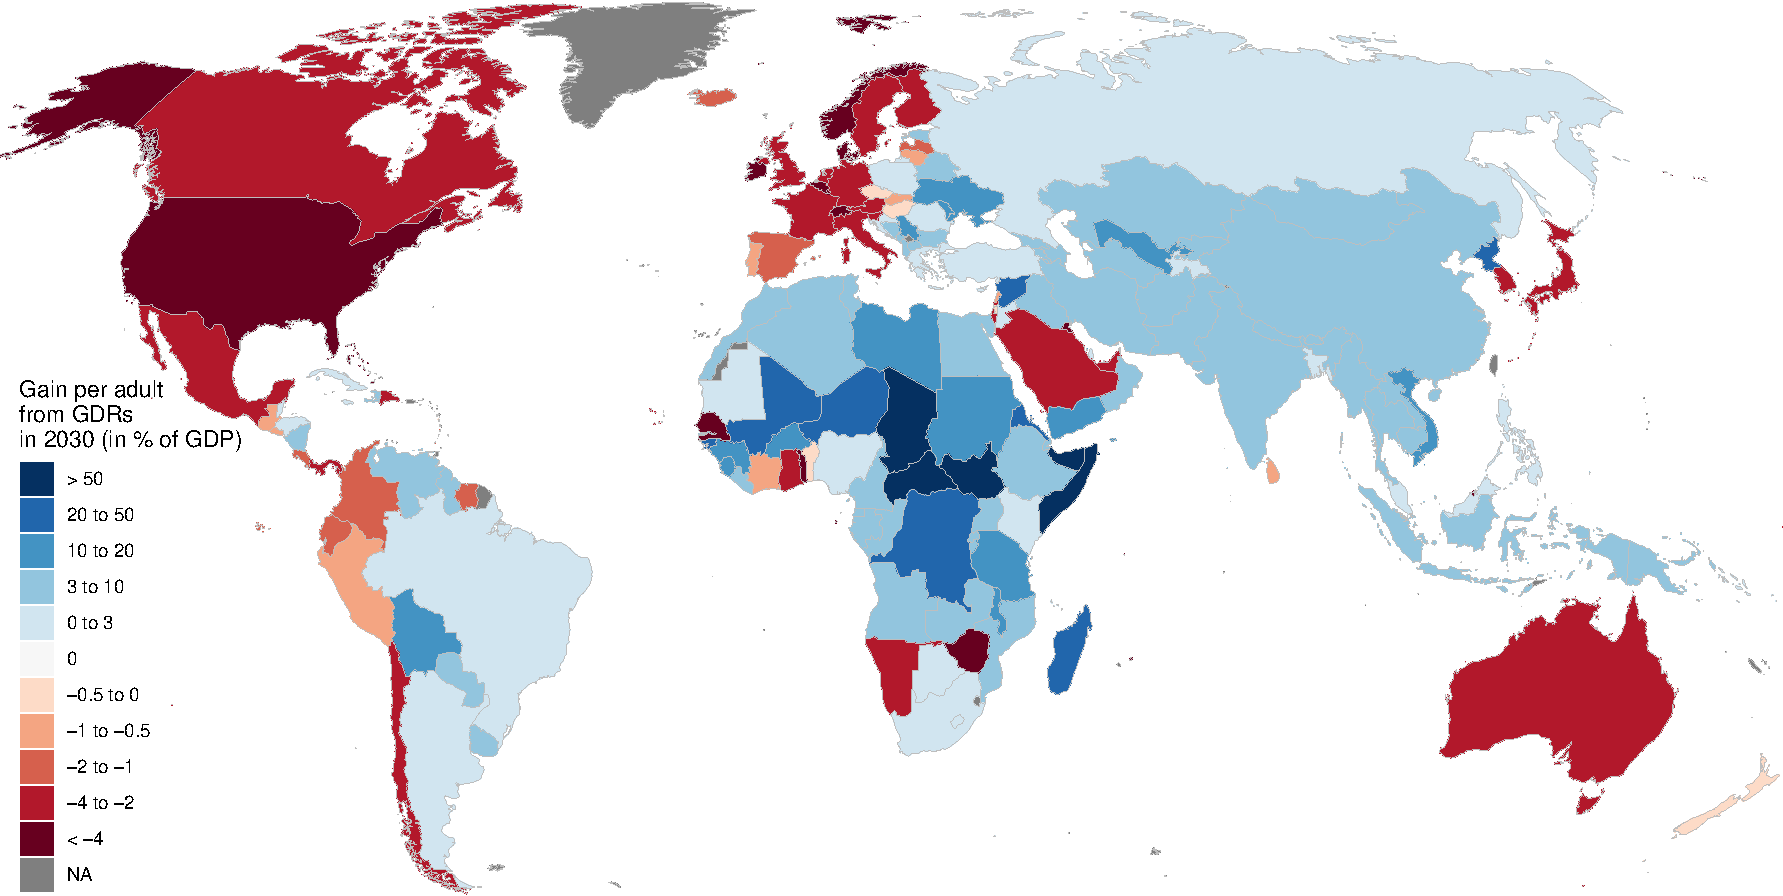
\includegraphics[width=\textwidth]{../figures/maps/gain_gdr_over_gdp_2030.pdf}} 
    {\small \textit{Note:} GDRs are calibrated with the preferred parameters of the \href{https://usfairshare.org/}{U.S. Climate Action Network} \citeRp{athanasiou_fair_2022} using the Efficiency scenario (2\textdegree{}C with $>$50\% chance) of the Global Energy Assessment \citeRp{johansson_global_2012} and a price of \$144/tCO$_\text{2}$.}
\end{figure} 

\begin{figure}[h!]
    \caption[Comparison between GDR and equal per capita burden-sharing rules.]{Difference between net gains from Greenhouse Development Rights and equal rights per capita. }\label{fig:diff_gain_gdr_gcs_over_gdp_2030}
    \makebox[\textwidth][c]{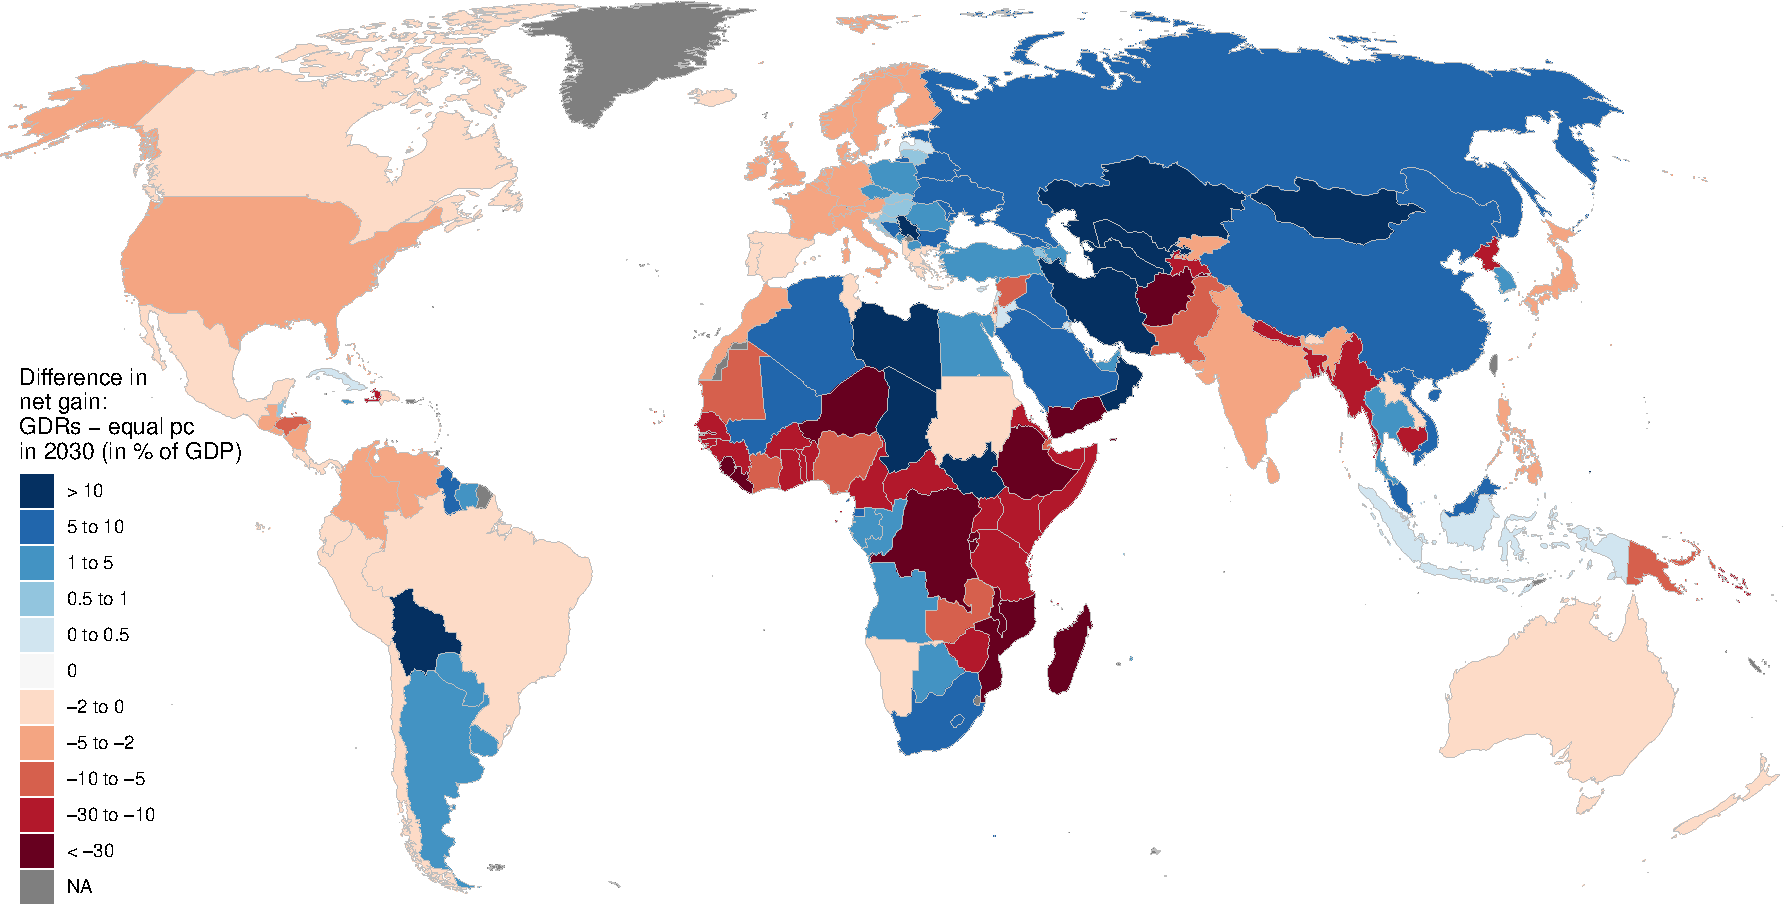
\includegraphics[width=\textwidth]{../figures/maps/diff_gain_gdr_gcs_over_gdp_2030.pdf}} 
    {\small \textit{Note:} GDRs are calibrated with the preferred parameters of the \href{https://usfairshare.org/}{U.S. Climate Action Network} \citeRp{athanasiou_fair_2022} using the Efficiency scenario (2\textdegree{}C with $>$50\% chance) of the Global Energy Assessment \citeRp{johansson_global_2012} and a price of \$144/tCO$_\text{2}$.}
\end{figure} % TODO? GDR -> CERF in figure?

\paragraph{Contraction and Convergence.} \citeRt{meyer_briefing_2004} defines a rule called \textit{contraction and convergence} (C\&C), which combines elements of grandfathering and equal per capita approaches. According to C\&C, each country is granted (tradable) emissions rights, starting at their current emission level and converging linearly to an equal per capita level at some pre-specified date. The \textit{contraction} part refers to the reduction of total emissions rights in line with the climate objective. When discussed around year 2000, the convergence date was specified between 2020 and 2050. This rule, advocated by the Global Commons Institute (a UK think tank), was on the agenda from COP2 to COP15 (i.e., until Copenhagen, and including in Kyoto), including at Kyoto, and was endorsed by the European Parliament in 1998. More recently, \citeRt{gignac_allocating_2015} have shown how C\&C can be made consistent with historical responsibilities by computing carbon debts and credits until the convergence date.

% TODO? There is also the "soft-landing" of Criqui et al. (14) used in POLES (hence also IMACLIM). C'est de la grosse tambouille.

\paragraph{Assessments of the NDCs against burden-sharing principles.} 
The regime established by the 2015 Paris agreement to regulate climate change respects none of the burden-sharing principles and relies instead on voluntary contributions from each country, known as Nationally Determined Contributions (NDCs). A body of literature (reviewed by \citeRalp{hohne_regional_2014}) assesses the NDCs against the emissions reduction objective and different burden-sharing principles. To evaluate the NDCs, \citeRt{gao_sufficient_2019} examine their emissions projections for 2030 and estimate the resulting increase in temperature. The most recent and comprehensive assessment of NDCs against burden-sharing principles is conducted by \citeRt{van_den_berg_implications_2020} (see also \citeRalp{raupach_sharing_2014}; \citeRalp{robiou_du_pont_national_2016}; \citeRalp{robiou_du_pont_equitable_2017}). 

%- Riahi et al. (17), Bauer et al. (17), Van Vuuren et al. (SSP1, 17), Kriegler et al. (SSP5, 16), Fricko et al (SSP2, 17): SSPs => Is SSP5 compatible with RCP2.6? Apparently, according to Riahi not really (Fig. 8) but it still appears in Bauer (Fig. 2) and Yes, according to Kriegler et al (17)
% Scenarios with low emissions:
% - SSP1/2/5-2.6 (or -1.9). (RCP1.9: 1.4°C en 2100 -> 1°C 2300 / 2.6: 1.8 °C -> 1.5 / 4.5: 2.7°C -> 3.3 https://global-climat.com/2021/09/02/rapport-ar6-du-giec-le-point-sur-la-temperature-globale/)
% - Global Energy Assessment (Johansson 12), e.g. Efficiency scenario
% - Greenpeace [Advanced] [R]evolution (Teske 15) 
% - NDCs (Gao et al 19). Check difference SSP2-4.5 with NDCs in 2030. Extend the NDCs either with SSP2 or with some assumption e.g. convergence to SSP2-2.6.
% - Decent Living: Kikstra et al 21
% - Low Energy Demand (Grubler): only has Global North and South
% - IEA ETP17 2DS and B2DS: doesn't have Africa nor GDP nor population
%- https://climateequitymonitor.in/ computes carbon debt based on equal per capita cumulative emissions. contact@climateequitymonitor.in https://twitter.com/equity4climate

% money/CO2 need to meet decent living standards: Kistra et al 21, Hallegatte et al 23 (TODO: read), Millward-Hopkins et al 20, Bruckner et al 22

\subsubsection{Global redistribution}\label{subsubsec:literature_redistribution}
% TODO? Give a stat on income disparities between countries?
% SDG, need for int'l transfers

\paragraph{Lack of cooperation vs. lack of redistribution.}
Major social science scholarship from Realism in International Relations to game theory of international environmental agreements in economics has pointed to lack of cooperation as the major obstacle to global sustainability (\citeRalp{waltz_theory_1979}; \citeRalp{snidal_relative_1991}; \citeRalp{barrett_self-enforcing_1994}; \citeRalp{nordhaus_climate_2015}). Another body of literature on international climate cooperation emphasises redistribution from North to South as a key condition for making global climate policy work, noting the historical responsibility of major emitters in the Global North (\citeRalp{parks_inequality_2008}; \citeRalp{friman_historical_2014}; \citeRalp{bou-habib_climate_2019}; \citeRalp{aklin_prisoners_2020}).  
Taking the second perspective, making progress on international climate policy also requires a decision on how the burden of climate change mitigation  can be shared fairly. This raises the question of whether citizens around the world support such global redistribution policies or, more specifically, whether citizens in high-income countries are willing to make sacrifices to combat climate change and extreme poverty.

While we cannot test conditional cooperation as part of the present analysis, our empirical results document that if the North-South redistribution would be implemented as part of global climate policies, they would receive strong public support.

\paragraph{Studies on global redistribution} 
Addressing global poverty, inequalities, and climate change are central to the universally agreed Sustainable Development Goals (SDG). % 12 out of  17
As highlighted by \citeRt{bolch_arithmetics_2022} and \citeRt{fabre_shortfall_2024}, low-income countries often lack sufficient domestic resources to eradicate poverty in the short term, indicating the need for international transfers to rapidly end global poverty. %In other words, it would hardly be possible to achieve the first SDG and end extreme poverty by 2030 without international transfers. % Zhang (16) estimates the poverty gap in each country. Global one is at $80G/year.
%This shows that international transfers would be needed to rapidly end global poverty. 
%The lack of solidarity from high-income countries has been long criticized. 
In \textit{Beyond the Welfare State}, Gunnar \citeRt{myrdal_beyond_1960} called for a \textit{welfare world}. In his Nobel lecture, he emphasized the necessity of increasing foreign aid to low-income countries, stating that ``The type of marginal foreign aid we have provided, is clearly not enough to meet their barest needs'' \citeRp{myrdal_equality_1975}.

% Unequal exchange, Hickel
Drawing on the labor theory of value, some economists have argued that global inequalities arise from unequal exchange in international trade \citeRp{arghiri_unequal_1972}. Indeed, the stark disparity in wages between countries implies that one unit of labor exported by an American commands five units of labor embodied in imported goods, whereas Ethiopians need to export 50 units of labor to obtain one unit through imports (\citeRalp{alsamawi_employment_2014}; \citeRalp{reyes_better_2017}).
Taking stock, \citeRt{hickel_divide_2017} proposes to globally establish minimum wages at 50\% of the local median wage. \citeRt{hickel_divide_2017} also suggests other solutions against global inequality, which served as inspiration for our questionnaire. These measures include the cancellation of low-income countries' public debt, fair trade practices (such as eliminating tariffs from high-income countries, reducing patent protections, and reducing farming subsidies in rich countries), initiatives to combat tax evasion (e.g., implementing a global financial register), land reform, and a fair international climate policy. 

\citeRt{piketty_capital_2014} prominently advocates for a progressive wealth tax on a global scale, and \citeRt{piketty_brief_2022} suggests to allocate its revenues to countries in proportion to their population. % although he does not specify whether the resulting revenues should fund international transfers. %how the revenues should be used, nor whether there should fund international transfers.% and it was implicit that each country would retain the revenues it collected. 

% Unfairness of current tax rates
\citeRt{kopczuk_limitations_2005} compute the optimal linear income tax rates for all countries in two ways: globally centralized and decentralized (i.e., within each country and without international transfers). They show that the average decentralized rate is 41\%. In contrast, the global rate is 62\%, which would generate funds to finance a basic income of 250\$/month (higher than the GPD per capita of 73 countries). From a current global Gini index of 0.695, they show that decentralized optimal taxation would only marginally reduce global inequality to 0.69, whereas global taxation would significantly decrease the Gini to 0.25. The study also shows that the existing level of foreign aid can only be rationalized if the U.S. attaches 2,000 less value to a citizen in the poorest countries than to an American citizen (or 1,000 less if half of the transfers are diverted due to corruption). 

% Carthy & Walsh (Oxfam, 22) propose various sources of funding for damages.
% Piketty (2014) "At what rate would [a global wealth tax] be levied? One might imagine a rate of 0 percent for net assets below 1 million euros, 1 percent between 1 and 5 million, and 2 percent above 5 million. Or one might prefer a much more steeply progressive tax on the largest fortunes (for example, a rate of 5 or 10 percent on assets above 1 billion euros). There might also be advantages to having a minimal rate on modest-to-average wealth (for example, 0.1 percent below 200,000 euros and 0.5 percent between 200,000 and 1 million)" He doesn't explicitly talk about revenue use, but implicitly they would be retained by each collecting country: "Le rôle principal de l'impôt sur le capital n'est pas de financer l'État social, mais de réguler le capitalisme.", "En principe, chaque pays de l'Union européenne pourrait obtenir des recettes du même ordre en appliquant seul un tel système."

\subsubsection{Basic income}\label{subsubsec:literature_basic_income}

Unconditional cash transfers (UCT) are increasingly seen as an effective way to end extreme poverty. A growing body of evidence from randomized control trials supports this notion: \citeRt{gangopadhyay_cash_2015} find that UCT outperform a food subsidy; \citeRt{haushofer_short-term_2016} find significant impacts on health, economic outcomes, and psychological well-being; \citeRt{egger_general_2022} find large positive spillovers on non-recipient people, and minimal inflation. 
Reviews of existing research further confirm the positive outcomes of UCT (\citeRalp{standing_little_2014}; \citeRalp{bastagli_cash_2016}). % TD: from the Cambridge dictionary, ``extant'' is ``used to refer to something very old that is still existing''', so I think ``existing'' fits better. Same comment applies to other occurrences of ``extant''.

While the delivery of cash to remote areas and the prevention of fraud is challenging in regions without a proper civil register, the use of mobile phones as banking and biometric identification tools could provide viable solutions \citeRp{harnett_taking_2017}. Although many places still lack internet access, satellite internet technology shows promising progress, with some experts suggesting that it could soon become affordable and universally accessible \citeRp{hanson_satellite_2016}.

\subsubsection{Global democracy}\label{subsubsec:literature_democracy}

The idea of world federalism has a long-standing history, dating back at least to \citeRt{kant_zum_1795}, who argued that a world federation was essential for achieving perpetual peace. 
International organizations were eventually created to foster peace, though the League of Nations and its successor, the United Nations, never succeeded in avoiding military conflicts. 
Many have argued that we need stronger and more democratic global institutions, competent to address global challenges such as extreme poverty, climate change, wars, pandemics, or financial stability. 
Before World War II, feminist and pacifist \citeRt{maverick_lloyd_chaos_1937} founded the \textit{Campaign for World Government}, advocating for direct representation at the global scale. 
\citeRt{einstein_general_1947} called for the subordination of the UN Security Council to the General Assembly and the direct election of UN delegates. 
Since 2007, there has been widespread support for a United Nations Parliamentary Assembly (UNPA) from individuals and institutions in over 150 countries, including 1,800 member of parliament, heads of state, as well the European Parliament, the Pan-African Parliament, and the Latin-American Parliament. The UNPA campaign calls for a gradual implementation of a democratic assembly, starting with a consultative assembly composed of members of national parliaments, allowing for the direct election of its members in voluntary countries, and progressing towards a world parliament with binding legislative powers once all members are directly elected \citeRp{leinen_world_2018}. % READ Ch 13, 21, 22, 26
Besides the UNPA, various scholars have put forward different models of global democracy, ranging from deliberative spaces to a world federation \citeRp{archibugi_global_2011}. 
While the most radical proposals may still be on the horizon, an assembly of random citizens representative of the world population has already been convened. It has produced a joint statement at the COP26 \citeRp{global_assembly_report_2022}, and a similar \textit{World Citizens' Assembly} should soon follow. Using surveys covering 86\% of global population, \citeRt{hale_could_2019} find that the world as a whole is less polarized that some countries and argue against the fear people's views would be too diverse for a functioning global democracy. % TODO READ and expand, also read marchetti_global_2008
%
% Stanford dico (kuyper_global_2016)? 

% ___________________________

% Burden-sharing
%- Agarwal & Narain (91) first to defend an equal right to emit per capita (equal to the absorbing capacity of the Earth)
%- Gampfer (14): lab experiment (ultimatum game) to test whether preferences respect fairness principles
%- Chancel & Piketty (15): global progressive carbon tax
% cf. bottom

% Global policies attitudes 
%* ISSP (19): Near consensus that “Present economic differences between rich and poor countries are too large.” p. 102, slight minorities (in rich countries) that “People in wealthy countries should make an additional tax contribution to help people in poor countries.” p. 104, but strong majorities everywhere that “People from poor countries should be allowed to work in wealthy countries.” p. 106
%* Ghassim et al. (22): support for stronger UN with more direct elections.
%* Ghassim (20):  in Germany those two parties that supposedly endorse global democracy – the Greens and the Left – benefitted, gaining nine and three percentage points respectively in terms of voting intentions. Meanwhile, the traditional centrist parties – SPD and CDU – each lost six percentage points due to their supposed opposition to global democracy.
%* Beiser-McGrath & Bernauer (19): Conjoint analysis in US, DE. Variant of carbon tax is 8 (US) - 17 (DE) p.p. more likely to be preferred and 50% more likely to be supported if tax is extended to all industrialized countries (Fig 1, 4). (Unfortunately, don't test extension to global level).
%- Çarkoğlu.. (15) International Social Survey Program 2010 data reveal that people in LDCs are less supportive of international agreements forcing their country to take necessary environmental measures than are citizens in the developed world [80% instead of 85%]. (‘for environmental problems, there should be international agreements that [their country] and other countries should be made to follow.’)
%* Carattini et al. (Nature, 19): 1k in US, IA, ZA, AU, UK. Each respondent receives one variant at random of global carbon price of 40/60/80 $/t redistributed as international dividend / national dividend / mitigation in all countries / mitigation in developing countries / domestic mitigation / reduced labour tax. Immense majorities for any scheme in India, small majorities for each elsewhere except US international dividend (44%) or mitigation in developing (43%), and AU mitigation in developing (49,6%). PB: very low sample size (~167) for a given redistribution, even lower (~55) for a given variant (that also specifies the price). Appendix also contains estimation of distributive impacts. Representative only along the two quotas: gender and age. Don't give the representativeness in terms of income (the third socio-demos that they ask) so it's probably bad.


% Global policies
%* Beyond the welfare state: Myrdal 58
% Pottier et al (17): A survey of global climate justice 
%* Hickel (17): The Divide: A Brief Guide to Global Inequality and its Solutions
%* Kopczuk et al (EER, 17) Compute optimal linear tax rate for all countries in two ways: decentralized or globally. Shows that the tax rate increases with inequality of skills (calibrated with the gini). The average decentralized rate is 0.41 The global one 0.62, with a global demogrant of 250$/month (higher than 73 countries' GDP). Show that within decentralized/country optimal taxation would not decrease global inequality by much (gini from 0.695 to 0.69, but down to 0.25 with global income tax). Show that USA don't give a damn of poor countries' people. citizens in the US (one of the richest) attach only 1/(2,000\*a) of the weight to the welfare of citizens in poorest countries, where a is the share  of transfer (supposedly) effectively arriving to the recipients. e.g. if half of aid is wasted by corrupt politicians, the weight is 1/1000.
% Carthy & Walsh (Oxfam, 22) propose various sources of funding for damages.
% Piketty (2014) "At what rate would [a global wealth tax] be levied? One might imagine a rate of 0 percent for net assets below 1 million euros, 1 percent between 1 and 5 million, and 2 percent above 5 million. Or one might prefer a much more steeply progressive tax on the largest fortunes (for example, a rate of 5 or 10 percent on assets above 1 billion euros). There might also be advantages to having a minimal rate on modest-to-average wealth (for example, 0.1 percent below 200,000 euros and 0.5 percent between 200,000 and 1 million)" He doesn't explicitly talk about revenue use, but implicitly they would be retained by each collecting country: "Le rôle principal de l'impôt sur le capital n'est pas de financer l'État social, mais de réguler le capitalisme.", "En principe, chaque pays de l'Union européenne pourrait obtenir des recettes du même ordre en appliquant seul un tel système."

% Global carbon pricing TODO find current advocates of GCS
%* Grubb (90), Betram (92) advocate for global market with equal pc right
%* Bergh et al. (20) call for a "dual-track transition to global carbon pricing": an expanding climate club, and "a reorientation of UNFCCC negotiations creates room for talking seriously about a global carbon price schedule, including redistribution-of-revenues rules." They don't specify which equity rules to use.
%* Jamieson (01) advocates of equal pc burden-sharing (after the precursors Agarwal & Narain (91))
%* Bear et al (Science, 00), Bear (02), Athanasiou & Baer (02) advocate for equal pc burden-sharing (although weirdly, Bear & Athanasiou then change mind and advocate for the Greenhouse Development Rights, accounting for capacity and responsibility)
%* Cramton et al (17): Livre de pontes. Tout le monde est d'accord : un prix mondial du carbone est requis, il ne peut être obtenu que par la réciprocité des engagements (style climate club), et il faut quelques transferts des riches vers les pauvres ainsi que des sanctions commerciales pour aligner les incitations. Ch 4 (also Cramton et al 15) propose la formule suivante de transfert (positif ou négatif) à un fonds climat : générosité*émissions en excès (par rapport à la cible)*prix du carbone. On demanderait aux États autour de la moyenne d'émission de fixer ce paramètre de générosité, pour qu'il soit fixé de sorte à maximiser le prix, puis on fixerait le prix comme le prix minimum proposé (après avoir éjecté qqs pays récalcitrants des négos). Puis, sanctions commerciales pour ceux qui ne respectent pas le prix. Ch Gollier & Tirole proposent une formule aussi simple que l'autre : quota global*((1-g)*part des émissions à t=0 + g*part de la population), où g joue le même rôle de paramètre de générosité/éthique (que je voudrais mettre à 1, mais qu'ils disent tous de mettre < 1 pour que les pays riches acceptent. Le livre argumente bcp sur prix vs. quantité (TLM préfère prix sauf Gollier & Tirole), l'argument le plus convaincant en faveur du prix c'est qu'avec la procédure proposée le prix négocié serait le plus élevé possible, alors qu'avec la quantité c'est le budget carbone qui serait le point focal et ça aboutirait à une impasse (objectif trop ambitieux).
% Blanchard & Tirole
%* MacKay et al (Nature, 15) summarizes the above
%* Weitzman (17) advocates for a World Climate Assembly, choosing the price level with the median voter, and each country retaining the revenues.
% Fleurbaey & Zuber (13): The discount rate converges to the worst-off (affected by the measure) to the worst-off (beneficiary of the measure) discount rate, which depends on the growth between both agents. Applied to real data, we can consider that the worst-off affected by a global tax on CO_2 is the average-earner on earth (around 75% centile i.e. ~1000€/month, cf. Chancel & Piketty, Lakner & Milanovic, Chakravorty) while the worst-off beneficiary is the worst-off person in the future (among those less affected by CC thanks to the measure), probably below 1000€/month => negative discount rate.
% Stanton (11): Negishi weights obviate the IAMs’ equalization of income. 4 ways to solve this problem: 1. be more transparent, 2. stop weighting, 3. take linear utility (i.e. maximize global GDP), 4. stop optimizing. 
% Hoel (91): Shows that an international tax can be designed so that it is both efficient and satisfies whatever distributional objectives one might have.
% IMF (2019): global pricing (with either differentiated prices or international transfers) or, as a first step, a carbon price floor. 25% of revenues should be rebated to the bottom 40%, the rest used to reduce distortionary taxes or for green investments. Estimate that $75/t is needed in 2030 for 2°C.
% Parry et al (21): Proposal for an International Carbon Price Floor Among Large Emitters. Acknowledges that transfers could be necessary to induce climate action in low/middle-income countries, talks about transferring 1% of carbon revenues.
%- Sager: distributive effects of global pricing without int'l transfers.
%- Budolfson et al. (incl. Fleurbaey, Méjean, Zuber, Dennig) (21): global carbon price with within-country per capita dividend. Acknowledge that "The overall benefits to society are even greater if total carbon tax revenues are returned on an equal per capita basis globally, which directs more of the revenues towards the poorest populations in the world (rather than the poorest within each country or region)." Very short (3p, no appendix, no suppl. info)

% Foreign aid 
%* Kaufmann et al (12) Shows the level of perceived and desired aid in 26 countries between 2005 and 2008 (cf. Table 1). In most countries (incl. UK, DE, FR, ES but not U.S.) desired aid is larger than perceived. Argue that this is due to political influence efforts/possibilities of the rich, as they prefer less aid due to vested interests (support this by a theoretical model + correlations between level of lobbying and actual aid level, controling for desired aid). In most countries the gap between the two is small, except in the U.S. where perceived is 7.5% of GDP and preferred is 3%.Use WVS and Gallup (like Chong & Gradstein, Paxton & Knack) but have more waves and the others don't use the question on perceived aid. Shows that richer want less aid ("those in the top income quintile favour ODA (as a share of GNI) that is 0.13 percentage points lower than the preferred share for individuals in the bottom 40\% of the income distribution" after controling for perceived aid - our regression results are sensibly the same.). from 0 to higher than 25%: threshold at 0.05; 0.15; 0.35; 0.75; 1.5; 2.5; 4; 7.5; 17.5; 25, i.e. same number of thresholds but small than ours below 2.5 and higher above. 
%*? Milner & Tingley (13): (highly cited but no original data, don't think we need to cite it) In 2008, 44% of American wanted foreign aid cut (american elections study, 08). fraction of federal budget going to foreign aid (mean: 27%, median: 25%) / should go (mean: 13%, median: 10%) (WorldPublicOpinion, 10)
% PIPA (01): Overwhelming majorities support a multilateral effort to cut hunger in half by the year 2015 and say that they would be willing to pay for the costs of such a program. However, most do not think that the average American would be as willing to pay the necessary costs. when PIPA asked respondents to estimate how much of the federal budget was devoted to foreign aid, the median estimate was 15% -- 15 times the actual amount, which was just under 1%. More dramatically, when asked what an appropriate percentage would be, the median response was 5% -- 5 times the actual amount. And when asked to imagine that they heard the real amount was only 1%, only 18% of respondents said they thought that would be too much--as compared to the 75% who had initially said that the US was spending too much. what percentage of their "tax dollars that go to help poor people at home and abroad...should go to help poor people in other countries." The mean response was 16% (down a bit from 22% in response to this question in a 1996 PIPA poll). Strikingly, this turns out to be a far higher percentage than is currently given. In 1999, a bit less than 4% of the total spent on the poor went to the poor abroad. Sixty percent of respondents proposed a percentage that was higher than 4%.
%- DFID (10): Priorities: 1 NHS, 2 education, 3 support to poor countries, 4 police, 5 defence (p. 19). Show majority support for increased aid until 07, then median is to support stable aid (due to crisis?). It seems they don't give the info on actual amount though.
%* PIPA (08): Across 20 countries, 81% support that "developed countries have a moral responsibility to help reduce hunger ansevere poverty in poor countries (majority in every country). “the World Bank (Shantayanan et al, 2002) has estimated that it will require an extra US$39-54 billion per year to meet Millennium Development Goal 1 (MDG1). (…) The per person cost of meeting MDG1 came to £25 for the UK, $56 for the US, €27 for Germany, and so on. On average 77 per cent of respondents are in favour of contributing towards meeting the goal (provided that all others do too). To take the US example, 75 per cent of people supported paying an extra $56 per year to meet MDG1. What is significant about this figure is that it is only slightly below the support for the ‘cost free’ question as to whether the US should be willing to share a  small portion of its wealth with those who are in great need (79%).” Hudson & van Heerde (12)
%* Hudson & van Heerde (12):Reviews literature on foreign aid and criticizes it on a number of points (e.g. not uncovering the determinants, and not asking well the questions). Shows strong support for poverty alleviation, (at least partly) out of intrinsic altruism. Use 4 main sources: PIPA (01, 08) UK DIDP, Eurobarometer; cf. Table 1 for all surveys on foreign aid / Public support for development has been famously described as a mile wide and and inch deep (Smillie, 1996: ref impossible to find). Hard times at home have meant that public support appears to have turned against international development efforts (Henson and Lindstrom, 2010). / Monitor public support: (Fransman and Solignac Lacomte, 2004; McDonnell et al, 2003), Paxton and Knack, 2008; Chong & Gradstein 2006. Review surveys on aid. / ~75% support aid in developed countries (stable) but ‘84 per cent agreed with the assertion that ‘taking care of problems at home is more important than giving aid to foreign countries’ (PIPA, 2001:9).” / References on covariates of aid support / PIPA 2001, "On average, Americans thought just under 25 per cent of the US budget was allocated to foreign aid, and government should allocate less than 14 per cent of the national budget. However, when told that US spends approximately 1 per cent of the federal budget on foreign aid, 37 per cent of respondents thought this was too little, 44 per cent thought it was about right, and 13 per cent thought it too much."  Think that only 23% of aid really goes to the poor / “The 2009 UK survey, Public Attitudes towards Development, reports ‘public support for overseas aid’ at 72 per cent (DFID, 2009); while in the US support was a comparable 79 per cent (PIPA, 2001); and average support across the EU trends slightly higher than in the US and UK with 91 per cent saying it was either very (53%) or fairly (38%) important to provide aid to poor countries (Eurobarometer, 2005).” / “DFID has now begun asking questions that provide relative measures of the salience of development aid vis-à-vis other competing policy issues (DFID, 2009; IDC, 2009). / "high proportion (61%) of US citizens who felt that the US spends too much on foreign aid. [from another source]” / “The distinction between foreign aid, which includes military spending, and development aid/assistance is an important one” / “81 per cent of respondents believed that developed countries do have a moral responsibility to work towards reducing hunger and severe poverty (WorldPublicOpinion.org, 2008). (…) there are a good number of people who support aid despite the fact they do not think it works. What this suggests – but cannot show in any detail – is that people have nonutilitarian motives for supporting aid.” / “support for development assistance is highly contingent on respondents’ perceptions of the effectiveness of aid, especially with regard to corruption (Henson et al, 2010). For example, in the UK, 47 per cent of respondents thought that aid was wasted, with sizable majorities citing corruption and poor management and/or delivery as primary factors (DFID, 2008). More disconcertingly, US respondents thought that only 23 per cent of US aid money that goes to poor countries ends up helping the people who really need it and 54 per cent of US aid money that goes to poor countries ends up in the pockets of corrupt government officials (PIPA, 2001). (…) international charities and NGOs are deemed best suited/most effective compared to donor countries” / UK ‘MyAid’ plan – where the public gets to vote on how a pot of money should be distributed – / "public engagement should be about ‘opening up the political and wider societal space to the possibility of deeper change’ (Darnton and Kirk, 2011:14).”
%* Gilens (01) 17% fewer American with high political knowledge want to cut foreign aid when we provide them specific information about aid amount.
%- Chong & Gradstein (16): from WVS 95-99, 58% want that their country give more foreign aid (but misperceptions are not taken into account)
%* Bauhr et al (13): Support for aid is reduced by perception of corruption in recipient countries. However, this effect is reduced by the aid-corruption paradox (and other things): most corrupt countries need more help.
%- Nair (18): (lack of) Aid support in US driven by information on global distribution, because people underestimate their rank by 27 centiles and overestimate global median income by a factor 10.
%- Williamson (19): Public Ignorance or Elitist Jargon? Reconsidering Americans’ Overestimates of Government Waste and Foreign Aid. "Foreign aid" encompasses military spending, in the mind of American.
%- McDonnell et al (03) Public Opinion and the Fight against Poverty
%- Nair (16): preferences driven by worldviews rather than self-interest
%- Bodenstein & Faust (17): Determinants of support for aid conditionality. They are: perceived corruption in donor country, right-wing.
%- Scotto et al (17): We Spend How Much? Misperceptions, Innumeracy, and Support for the Foreign Aid in the United States and Great Britain. Less American and British want aid cut when information on current aid is given in % of GDP rather than in $.
%* Paxton & Knack (12): Majorities want more aid, and main determinants are trust, ideology, interest in politics, and female (all positive). Gallup 02: in US 45% want more aid (rather than stable) vs. 68-91 in DE-UK-ES. Like Chong & Gradstein, find that desired aid increases with income, contrary to Kaufmann et al. but the latter contains more datasets.
%- Wood (15): Determinants for aid support in Australia. Wood (18) Examine Australian support for aid: although there is support to help foreign poor, people back recent aid cuts.
%- Bayram (17): Aid support associated with trust, i.e. seeing integrity and trustworthiness in others.
%- Cheng & Smyth (16): Why Give it Away When You Need it Yourself? Understanding Public Support for Foreign Aid in China. Political ideology and patriotism main explaining variables for aid support. People in poorer provinces less supportive.
%- Milner & Tingley (10) theory + empirics: who supports aid and why. owners of capital in donor countries tend to gain from aid and thus are more likely to support giving aid
%- Easterly (JEP, 03) Can Foreign Aid Buy Growth? No (disproves Hansen & Tarp).
%- Hansen & Tarp (01) Aid increases growth (empirical evidence)
%- Tresch et al. (22): 66% of Swiss people want to increase their foreign aid; also Borofsky
%- Harris (17): majority of French want to decrease foreign aid


% Universalism
%- Enke et al. (Manag. Science, 23): measures universalism by asking to split donation to domestic and foreigner of same absolute income (US).
%- Enke et al. (ReStud, 23): unviersalism more correlated to policy attitudes than income, education, religiosity or beliefs about government efficiency (West).
%- Cappelen et al. (NBER, 22): how unviversalism (as measured above) varies across countries. Comparable in Europe and US (lower in China, higher in Africa)
%- Cherry et al (17) show in the lab that some people prefer policies detrimental to them due to their worldview.


% Free-riding
%- Mildenberg (2019): people are not free riders
%- McGrath & Bernauer (17): review paper. people are not free riders. Preferences concerning climate policy tend to be driven primarily by a range of personal predispositions and cost considerations, which existing research has already explored quite extensively, rather than by considerations of what other countries do
%- Bernauer & Gampfer (15): US and IA people are not free riders. They each overestimate their country's emissions at one third of global total.


% Social norms
%- Bursztyn et al. (AER, 20): social norms can change following new public information such as unexpected election outcome. After Trump election, people express more xenophobic views and judge less severely those who do.
%- Farrow et al. (17): review of effect of social norm intervention on environmental attitudes

% Incentive compatibility
%- Danz et al


% Second-order beliefs
%* Mildenberg & Tingley (19): survey elites (Congress staffers, scholars) and public in U.S. and China and show pluralistic ignorance of pro-climate attitudes, egocentric bias, and increasing support after beliefs are updated.
%- Bursztyn & Yang (21): Review of the field. Misperceptions about others are widespread, asymmetric, much larger when about out-group members, and positively associated with one’s own attitudes.
%- Drews et al. (22): in Spain, supporters (resp. opponents) of carbon tax overestimate (resp. underestimate) support. Providing information doesn't change the overall support.
%* Falk et al. (21): Respondents vastly underestimate the prevalence of climate- friendly behaviors and norms among their fellow citizens. Providing respondents with correct information causally raises individual willingness to fight climate change as well as individual support for climate policies. The effects are strongest for individuals who are skeptical about the existence and threat of global warming.
%- Di Tella et al. (AER, 15): The results of the lab experiment favor the hypothesis that people avoid altruistic actions by distorting beliefs about others' altruism
%- Allport (1924): first book on pluralistic ignorance
%- Allport (40): function of poll is to correct pluralistic ignorance
%- Studies on pluralistic ignorance: business (Buckley et al. 00), against affirmative action (Van Boven 00), political correctness (Braghieri, AER 21), alcohol (Suls & Green, 03), white support for racial segregation (O'Gorman 75), CC (Geiger & Swim 16), hooking up (Lambert et al 03, cf. note for paragraph of pluralistic ignorance), women working outside home in Saudi Arabia (Bursztyn et al. 20)
%- Geiger & Swim (16) Shows that pluralistic ignorance of others' concern about CC leads people to talk less about CC and self-silence themselves.
%- Miller & MacFarland (87) Shows that pluralistic ignorance emerges because individuals believe that fear of embarrassment is a sufficient cause for their own behavior but not for the behavior of others.


% Elite surveys TODO find more
%* Mildenberg & Tingley (19): Congress staffers, cf. second-order beliefs
%- Hertel-Fernandez et al. (2019): Survey on US Congress staffers (not on climate)
%- Milner & Tingley (10) (not sure it's a survey) owners of capital in donor countries tend to gain from aid and thus are more likely to support giving aid
%- Lange et al. (Energy Econ, 2007): climate negotiators
%- Lange et al. (EER, 2010): same data as Lange et al. (10)
%- Dannenberg et al. (ERE, 2010): elicit climate negotiators’ equity preferences using Fehr & Schmidt (99) method => regional differences in addressing climate change are driven more by national interests than by different equity concerns
%- Kesternich et al. (EEPS, 2020): survey on climate negotiators about their preferred burden-sharing rules: we observe tendencies for a more harmonized view among key groups towards the ability-to-pay rule in a setting of weighted burden sharing rules
%- Lange & Schwirplies (ERE, 2017): combines Lange et al. (10) and Schleich et al.
%* Hjerpe et al. (2011): Delegates at COP2009. The results indicate that voluntary contribution, indicated as willingness to contribute, was the least preferred principle among both negotiators and observers. Three of the four principles for allocating mitigation commitments were recognized widely across the major geographical regions: historic 1990, capacity to pay, and equal per capita emissions. The difference was never below 25 percentage units, and the opponent share never exceeded 16%.
%- Scholte et al. (2020)
%- Bayram (17): cosmopolitanism of German politicians and their respect of international law


% Global poverty gap
%* Bolch et al. (22)
%- Zhang (16) estimates the poverty gap in each country. Global one is at $80G/year.


% Basic income 
%* Egger et al. (19): positive gen eq effects. We provided one-time cash transfers of about USD 1000 to over 10,500 poor households across 653 randomized villages in rural Kenya. The implied fiscal shock was over 15 percent of local GDP. We find large impacts on consumption and assets for recipients. Importantly, we document large positive spillovers on non-recipient households and firms, and minimal price inflation.
%* Haushofer & Shapiro (16): The Short-term Impact of Unconditional Cash Transfers to the Poor: Experimental Evidence from Kenya. Monthly transfers are more likely than lump-sum transfers to improve food security


% Unequal exchange / embodided labour
%- Reyes et al (17)
%- Sakai et al (17)
%- Alsamawi et al. 2014


% NDCs assessments or burden-sharing computations. 
%- Bourban (18): Soutient un marché du carbone avec droits en proportion des émissions cumulées depuis 1990. Et des “mesures volontaires de contrôle de la population mondiale”.
%- Raupach et al (NCC, 14): clear computations of regional carbon budget under different budget sharing
%- van den Berg et al (20): same
%- Meyer (04) Contraction and Convergence (i.e. grandfathering converging to equal pc, within an ETS)
%- AGBM 97: Contraction and Convergence proposed by France
%- >Baer et al (08)< (cite this one, others don't give more info), Baer (13), Athanasiou et al (22), Holz et al (19) https://calculator.climateequityreference.org/ Athanasiou, Greenhouse Development Rights, EcoEquity calculator, US fair share. Effort-sharing approach based on splitting emissions reductions in function of capacity to pay (~ share of global income in top 30%) and responsibility (share of emissions since 1950), weighted equally. Corresponds to UNFCCC wording. Pb of this method (applying to any choice of parameters): A country with relatively low incomes (e.g. equal distribution slightly above the p70) and that has few historical responsibility would have a relatively low effort. Even more problematic, the **poorest countries would have virtually 0% of the effort, hence they would be allowed to emit following the baseline trajectory… but this baseline is not fair; it amounts to grandfathering**. It is computed as the “product of the projected GDP and CO2 emission intensity”. ([https://climateequityreference.org/calculator-information/gdp-and-emissions-baselines/](https://climateequityreference.org/calculator-information/gdp-and-emissions-baselines/)), and give for example 0.8tCO2e/cap for RDC in 2030 (16% more than in 2020, but lot lower than the objective of ~4t). => Compared to an equal right to emit pc, this method favors countries like China (allowed to remain stable over 2020-30 vs. reduced by 35-40%) and penalizes countries like the U.S. and Africa. 
%  in Athanasiou et al (22) Justification of Greenhouse Development Rights instead of Equal per capita right is on p. 36. It is weak, and basically that historical responsibility should be taken into account. Conversely, justification against historical resp. is that the latter doesn’t take into account capacity to pay (it is not said like this, but we can think of ex-USSR).
%- Pachauri et al. (Science, 2022): "we find that distributive justice considerations in global climate mitigation will require substantial interregional finance flows" READ
%- Robiou du Pont et al. (NCC, 2017): China’s Nationally Determined Contribution (NDC) is weaker than any of the five equity approaches, India’s and the USA’s NDC are aligned with two, and the EU’s with three. … If the G8 and China adopt the average of the five approaches, the gap between conditional INDCs and 2 C-consistent pathways could be closed.
%- Robiou du Pont et al. (ERL, 2016): READ we identify global cost-optimal emissions scenarios from Integrated Assessment Models that match the G7 agreement [of reducing emissions by ~65% by 2050 compared to 2010, in line with >66% <2°C]. These scenarios have global 2030 emissions targets of 11%–43% below 2010, global net negativeCO2 emissions starting between 2056 and 2080 … G7 members’ Intended Nationally Determined Contribution (INDCs) mitigation targets are in line with a grandfathering approach but lack ambition to meet various visions of climate justice. The INDCs of China and Russia fall short of meeting the requirements of any allocation approach. Depending on how their INDCs are evaluated, the INDCs of India and Brazil can match some equity approaches evaluated in this study.
%- Höhne et al. (Climate Policy, 2014): review of 40 papers READ
%- Gao et al. (FEM, 2019): assesses NDCs
%- Gignac & Matthews (ERL, 15) READ
%- Matthews (16) Quantifying carbon debts among nations 
%- https://climateequitymonitor.in/ computes carbon debt based on equal per capita cumulative emissions. contact@climateequitymonitor.in https://twitter.com/equity4climate


% Mismatch between preferences and climate action TODO! cite
%- McCright & Dunlap (03) show that it's an organized conservative movement that succeeded in the U.S. not ratifying Kyoto, through lobbying and disinformation.


% Wealth tax attitudes
% look for surveys on global tax => I've found no result with survey or attitudes + "global tax" or "global wealth tax" in google scholar
% Fisman et al (17): Americans want a 3% tax on inherited wealth
%- Christensen et al. (Oxfam, 23) p. 32 gives references on rich tax attitudes, with always strong majority support:
%* OECD (19): 52-80% of absolute support for "government tax the rich more than they currently do in order to support the poor" in 21 OECD countries
%* Isbell (22): 34 African countries
%- Patriotic Millionaires (22), UK
%- Americans for Tax Fairness (21), US
%- Gallup (22), US
%- Fight Inequality Alliance India (22), IA

% Different framing of burden-sharing, depending on what should be split:
% - mitigation costs: this is the most used as it is easiest to explain. The issue is that it is not specified how agents pay (or if some agents receive payments) and implicitly, there is no negative costs (transfers exceeding the costs) and the carbon price is not uniform. Used in .
% - emission: this one is vague as it doesn't state at which date emissions pc converge (if they do) and whether there are side payments.
% - emission rights: this one is the most accurate as there is no need of a BAU scenario to compute the mitigation needed and its cost.

% Different fairness principles:
% - equal emission right per capita: using this as a baseline, we can call 'grandfathering' any principle that is more regressive and 'historical responsibility' any principle that is more progressive
% - equal emission reduction (in share of current emission) per capita: grandfathering
% - emission rights proportional to current emissions: grandfathering
% - costs proportional to current emissions: polluter-pay principle
% - costs proportional to cumulative emissions: so-called historical responsibility but may actually have a grandfathering component

% Surveys of population:
% - Schleich et al. (Climate Policy, 16) ask for ranking and find an identical ranking of fairness principles in China, Germany, and the US: accountability (costs according to emissions) followed by capability (according to economic strength), egalitarianism (equal emission per capita), and sovereignty (constant share of global emission) (see Lange & Schiwplies (17) for the computations). 
%   Polluter-pays: Every country has to bear costs according to the emissions it causes (hence countries causing higher emissions have a higher share of the costs).
%   Ability-to-pay: Every country has to bear costs according to its economic strength (hence richer countries have a higher share of the costs).
%   Egalitarian: Every country is allowed to produce the same amount of emissions per capita (hence countries with currently high emissions per capita have higher costs).
%   Sovereignty: Every country is allowed to produce the same share of global emissions as in the past (hence the proportional reduction of emissions is the same for every country).
% other findings: international agreements are important but current ones are unsuccessful, people find themselves poorly represented in climate negotiations
% - Bechtel & Scheve (PNAS, 13) find with a conjoint analysis on FR, DE, UK, US that a climate agreement is 5 p.p. less likely to be preferred (to a random alternative) if only rich countries pay (other burden-sharing are: pay prop. to current emissions / historical emissions / rich countries pay more than poor countries) and 15 p.p. more likely to be preferred if it includes 160 (out of 192) countries rather than 20 => confirms preference for global policies (rather than only partial coverage). Finds that costs is what matters most: preference decreases by 30pp if it’s 2.5% of GDP compared to 0.5%.
% - Carlsson et al. (REE, 13) find using a 09 choice experiment that Americans prefer capacity to pay > current responsibility > historical responsibility > equal emissions per capita while Chinese prefer historical > capacity > current > equal emissions.
%   Capacity to pay: Countries with high income levels must pay a larger share of the costs than countries with low income levels. This option says that countries with greater ability to pay should pay more
%   Current responsibility: Countries with currently high emissions levels must pay a larger share of the costs than countries with currently low emissions levels. This option says that those countries that are currently a larger part of the problem should pay more.
%   Historical responsibility: Countries with a history of high emissions levels must pay a larger share of the costs than countries with a history of lower emissions. This option recognizes that CO2 builds up in the atmosphere over many years. Thus, countries with a history of high emissions should pay more because they caused more of the problem.
%   Equal emissions pc: Countries with emissions per person greater than an agreed amount must pay, and they must pay more the higher their emissions per person area.
% > "equal emissions" is a misnomer as this is about costs (not emissions) and it's just a more progressive version of current responsibility / polluter-pay, where high-emitting pay more and low-emitting don't pay. The result for US is compatible with the other papers as Americans agree that rich countries (or high-emitting, the diff is small) should pay more. The Chinese position could also be reconciliable once we define responsibility from footprint rather than territorial and that there will be transfers from rich to poor countries.
% - Carlsson et al. (Ecol Eco, 11) find that Swedes prefer that "all countries are allowed to emit an equal amount per capita" rather than options where emissions reduce in relation to current or historical emissions and continue to be higher in high-emitting countries. 
% - Meilland et al. (23) find that in US and France, most favored fairness principle is Equality in per capita emissions: "all countries commit to converge to the same average of total emissions per inhabitant, compatible with a controlled climate change" and second-most (which closely follows) is grandfathering: "all countries commit to reduce their emissions by a same proportion". 73% in each disagree with grandfathering when defined as "countries which emitted a lot of carbon in the past have a right to continue emitting more than others in the future". To rationalize these contrasted views with grandfathering, we can interpret them as: equal rights, equal emission reductions, and transfers. 
%   convergence per capita (70%): all countries commit to converge to the same average of total emissions per inhabitant, compatible with a controlled climate change
%   grandfathering (60%): all countries commit to reduce their emissions by a same proportion
%   past emissions (20% choose it among their two favorite): countries which emitted less in the past commit to reduce their emissions less than other countries
%   poor countries (20%): poorer countries commit to reduce their emissions less than richer countries
%   cost-efficiency (20%): countries where reducing emissions is more costly commit to reduce their emissions less than other countries
% Other findings: people prefer international settlement on CC even if it empedes on sovereignty, a majority prefers to target footprint rather than territorial emissions, median is that countries should be held accountable for post-1990 emissions, self-serving bias when judging e.g. India vs. EU, no shared understanding of fairness when asked to coordinate between French and Americans
% - Dechezleprêtre et al. (WP, 22) find that equal per capita right > historical responsability, capabilities > grandfathering; that global CC policies are needed; 50% support for global T&D; strong support for global tax on millionaires; no free-riding. 
% - Dabla-Norris et al. (WP, 23) find strong majority for “all countries” everywhere in “Which countries do you think should be paying to reduce carbon emissions?”, and majority for current rather than historical in all countries but China and Saudi Arabia in “Should countries be paying to reduce carbon emissions based on their current or accumulated historic levels of emissions?”

% > Position making all this compatible: people want that every country engage in strong decarbonization effort together, with a global quota, converging to climate neutrality in the medium run, based on an equal right to emit per person, implying that rich countries pay and low-emitting countries receive funding. Where the rankings differ, it is likely because the definitions or wordings are different, and also because it involves different countries (Sweden != US != China).
% - Schleich find support for costs according to emissions and against immediate equalization of emissions (but nothing against convergence to equal emissions per capita).
% - This is just in contradiction with Carlsson (11) which finds that Swedes prefer the equalization (with a similar wording) to other reduction options. 
% - Bechtel find agreement that rich countries should pay more and historical emissions matter, but just that they should not be the only one to make the efforts. 
% - Carlsson (13) find that the least preferred option in China and US is when low-emitting countries don't participate to the effort. Ability to pay is liked in both countries.
% - Meilland find that convergence is the most preferred, followed by emission reductions of same proportion, disagreement with grandfathering expressed in terms of emission rights.
% - Dechezleprêtre find support for equal right is strongest, although historical responsibility and capabilities are also supported. The quota system is strongly supported.

% Surveys of negotiators:
% - Hjerpe et al. (WP, 11)
% - Dannenberg et al. (ERE, 10): measuring negotiators' equity preferences, regional differences in addressing climate change are driven more by national interests than by different equity concerns.
% - Lange et al. (Energy Econ, 07): Mix of self-serving bias and support for egalitarian principle.
% - Kesternich et al. (EEPS, 21): kind of convergence on ability-to-pay.

% Other papers:
% - Lange & Schwirplies (ERE, 17) develop a theoretical model (building on Buchholz et al. (05)), supported by data, justifying that climate negotiators (chosen by the citizens) have lower environmental preferences than their citizens and equity views more aligned with the other negotiators. 
% - List experiment: Kuklinski et al. 97 or https://blogs.lse.ac.uk/europpblog/2022/04/06/do-russians-tell-the-truth-when-they-say-they-support-the-war-in-ukraine-evidence-from-a-list-experiment/
\clearpage
\section{Raw results% from the complementary surveys
}\label{app:raw_results}
% /!\ Do not replace by app_desc_stats_US1 as the latter also contains figures that are already in the main text
% TODO? add country-specific prioritization? No, it's in (separate) country appendices.
% TODO! add share who click on info or reminder
% TODO! Appendix Sources or at least clean up specificities.xlsx

For each figure, the captions refer to the figure's \verb|filename| and to the questionnaire's question. The figures' folders are \verb|figures/country_comparison| (for PDFs) and \verb|xlsx/country_comparison| (for data tables), except when the filename contains a folder name (which then replaces \verb|country_comparison|). 
Country-specific raw results are also available as supplementary material files:  \href{https://github.com/bixiou/international_attitudes_toward_global_policies/raw/main/paper/app_desc_stats_US.pdf}{US}, \href{https://github.com/bixiou/international_attitudes_toward_global_policies/raw/main/paper/app_desc_stats_EU.pdf}{EU}, \href{https://github.com/bixiou/international_attitudes_toward_global_policies/raw/main/paper/app_desc_stats_FR.pdf}{FR}, \href{https://github.com/bixiou/international_attitudes_toward_global_policies/raw/main/paper/app_desc_stats_DE.pdf}{DE}, \href{https://github.com/bixiou/international_attitudes_toward_global_policies/raw/main/paper/app_desc_stats_ES.pdf}{ES}, \href{https://github.com/bixiou/international_attitudes_toward_global_policies/raw/main/paper/app_desc_stats_UK.pdf}{UK}.

\begin{figure}[h!]
    \cprotect\caption[Support for the Global Climate Scheme]{Support for the GCS, NR and the combination of GCS, NR and C (\textit{Yes}/\textit{No} questions). \\(\verb|support_binary_positive|; p. \pageref{subsec:questionnaire_GCS}, Questions \ref{q:gcs_support}, \ref{q:nr_support}, \ref{q:global_tax}, \ref{q:national_tax}, and \ref{q:crg_support}).%; $n_\text{US} = n_\text{Eu} = 3,000,\, n_\text{FR} = 729,\, n_\text{DE} = 929,\, n_\text{ES} = 543,\, n_\text{UK} = 749$)
    }\label{fig:support_binary}
    \makebox[\textwidth][c]{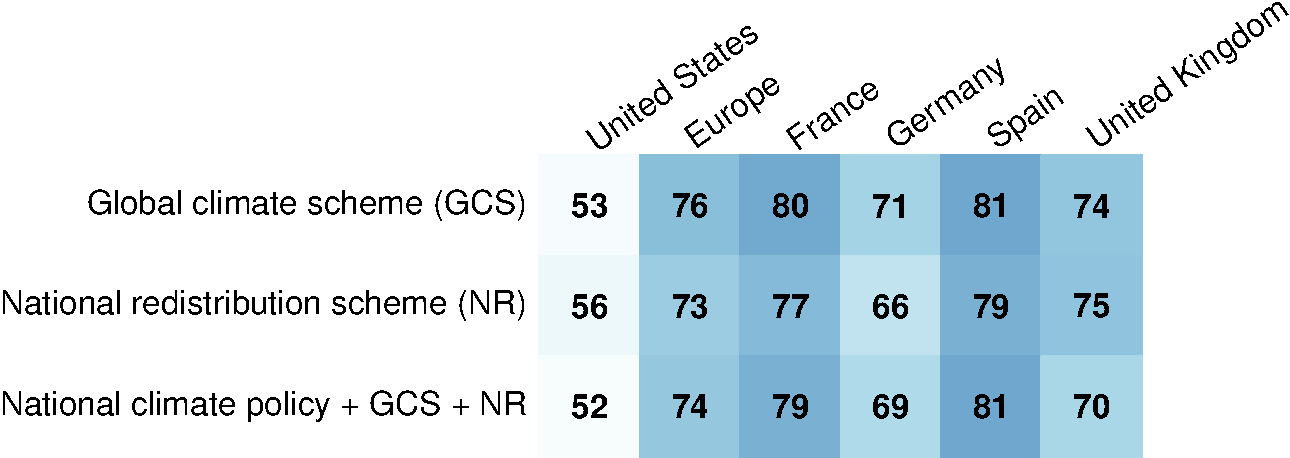
\includegraphics[width=.9\textwidth]{../figures/country_comparison/support_binary_positive.pdf}} 
\end{figure}

\begin{figure}[h!]
    \cprotect\caption[Absolute support for global climate policies]{Absolute support for global climate policies. \\ Share of \textit{Somewhat} or \textit{Strongly support} (in percent, $n$ = 40,680). The color blue denotes an absolute majority. See Figure \ref{fig:oecd} for the relative support. (\verb|OECD/Heatplot_global_tax_attitudes_positive|; Questions \ref{q:scale}-\ref{q:millionaire_tax} of the global survey.)% Reproduced from \citealp{dechezlepretre_fighting_nodate}, Figure A20.)
    } 
    \makebox[\textwidth][c]{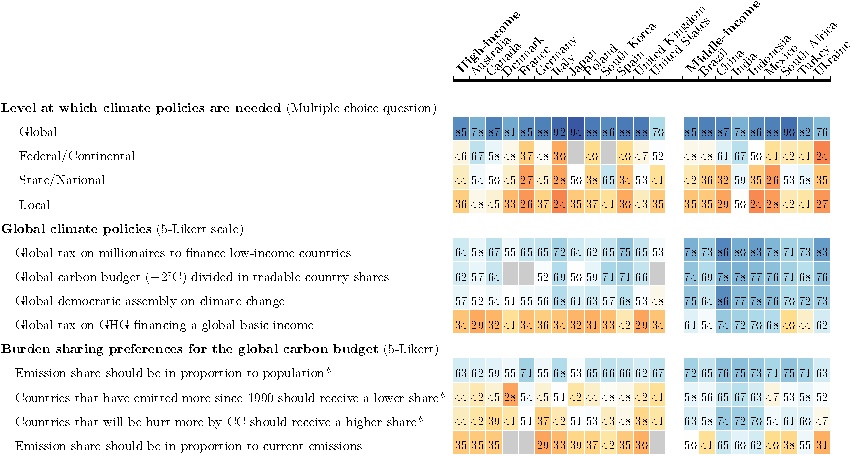
\includegraphics[width=1.2\textwidth]{../figures/OECD/Heatplot_global_tax_attitudes_positive.pdf}}\label{fig:oecd_absolute}% with dependence on others (absent from OECD): Heatplot_burden_share_all_positive_countries
    {\footnotesize \\ *In Denmark, France and the U.S., the questions with an asterisk were asked differently, cf. Question \ref{q:burden_sharing_asterisk}. } 
\end{figure}

\begin{figure}[h!]
    \cprotect\caption[Comprehension]{Correct answers to comprehension questions (in percent). (\verb|understood_each_positive|; Questions \ref{q:understood_gcs}-\ref{q:understood_both})}\label{fig:understood_each}
    \makebox[\textwidth][c]{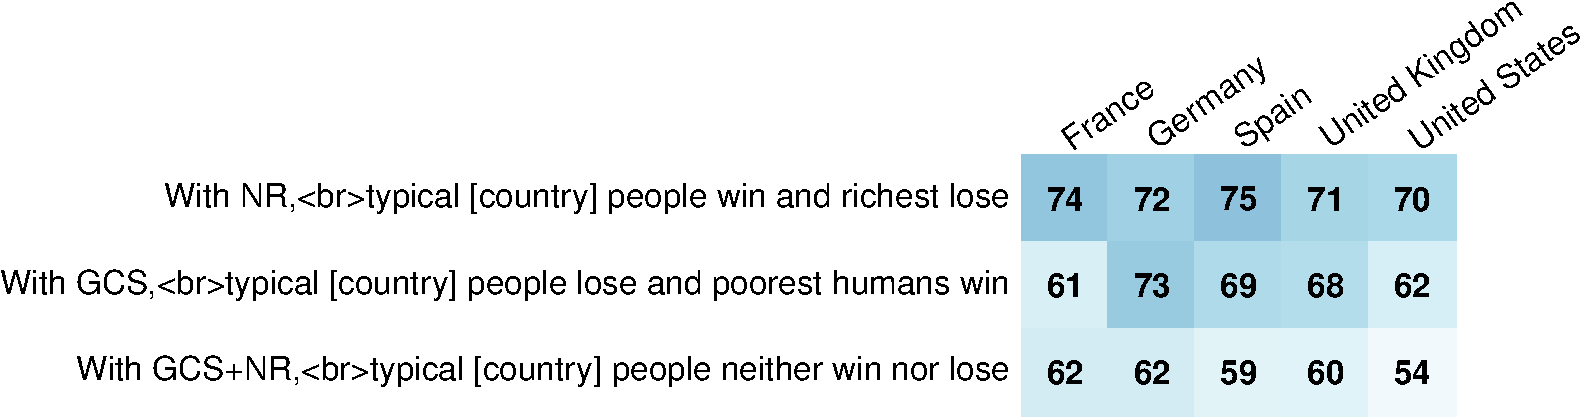
\includegraphics[width=\textwidth]{../figures/country_comparison/understood_each_positive.pdf}} 
\end{figure}

\begin{figure}[h!]
    \cprotect\caption[Comprehension score]{Number of correct answers to comprehension questions (mean). (\verb|understood_score_mean|; %Section \ref{subsec:gcs_stated_support}, 
    Questions \ref{q:understood_gcs}-\ref{q:understood_both})}\label{fig:understood_score}
    \makebox[\textwidth][c]{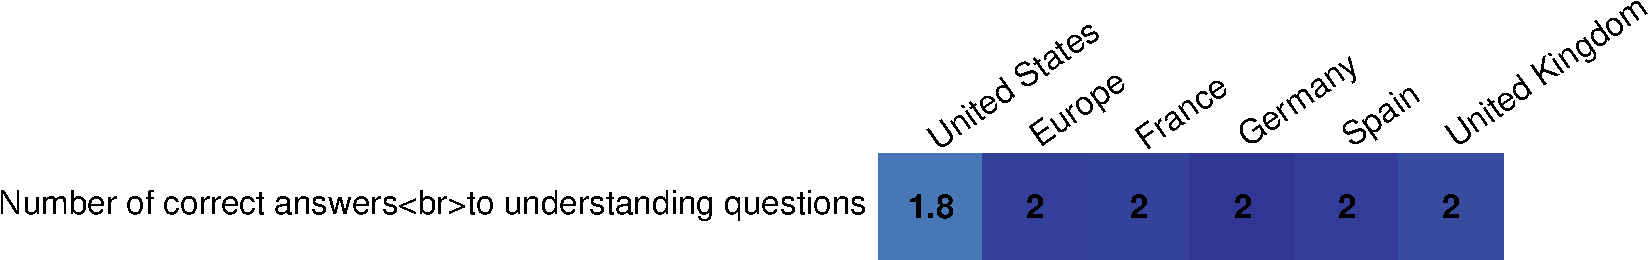
\includegraphics[width=\textwidth]{../figures/country_comparison/understood_score_mean.pdf}} 
\end{figure}

% \begin{figure}[h!]
%     \cprotect\caption[Support for the Global Climate Scheme]{Support for the GCS, NR and the combination of GCS, NR and C. (Questions \ref{q:gcs_support}, \ref{q:nr_support} and \ref{q:crg_support})}\label{fig:support_binary}
%     \makebox[\textwidth][c]{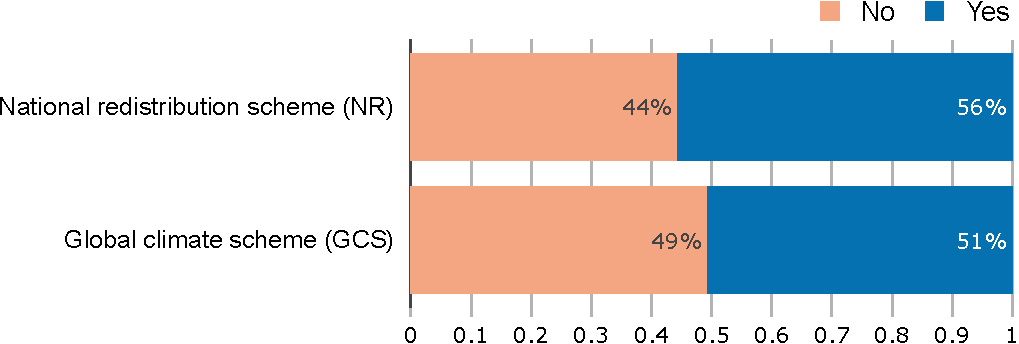
\includegraphics[width=.9\textwidth]{../figures/country_comparison/support_binary.pdf}} 
% \end{figure}

% \begin{figure}[h!]
%     \cprotect\caption[Beliefs about support for the GCS and NR]{Beliefs regarding the support for the GCS and NR. (Questions \ref{q:gcs_belief} and \ref{q:nr_belief})}\label{fig:belief}
%     \makebox[\textwidth][c]{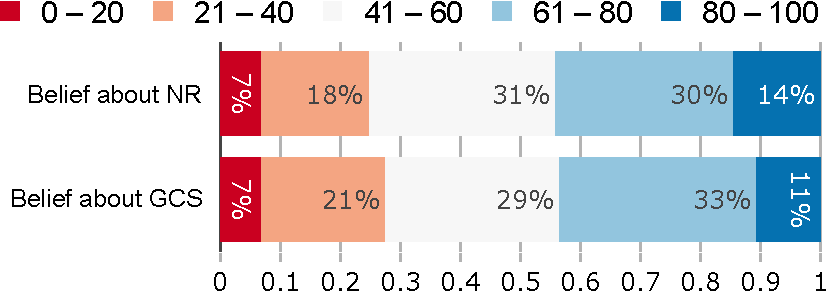
\includegraphics[width=.8\textwidth]{../figures/country_comparison/belief.pdf}} 
% \end{figure}

\begin{figure}[h!]
    \cprotect\caption[List experiment]{List experiment: mean number of supported policies. (\verb|list_exp_mean|; %Section \ref{subsubsec:list_exp}, 
    Question \ref{q:list_exp})}\label{fig:list_exp}
    \makebox[\textwidth][c]{
\includegraphics[width=.7\textwidth]{../figures/country_comparison/list_exp_mean.pdf}} 
\end{figure}

\begin{figure}[h!]
    \cprotect\caption[Conjoint analyses 1 and 2]{Conjoint analyses 1 and 2. (\verb|conjoint_ab_all_positive|; Questions \ref{q:conjoint_a}-\ref{q:conjoint_b}%, Back to Section \ref{subsubsec:conjoint}
    )}\label{fig:conjoint}
    \makebox[\textwidth][c]{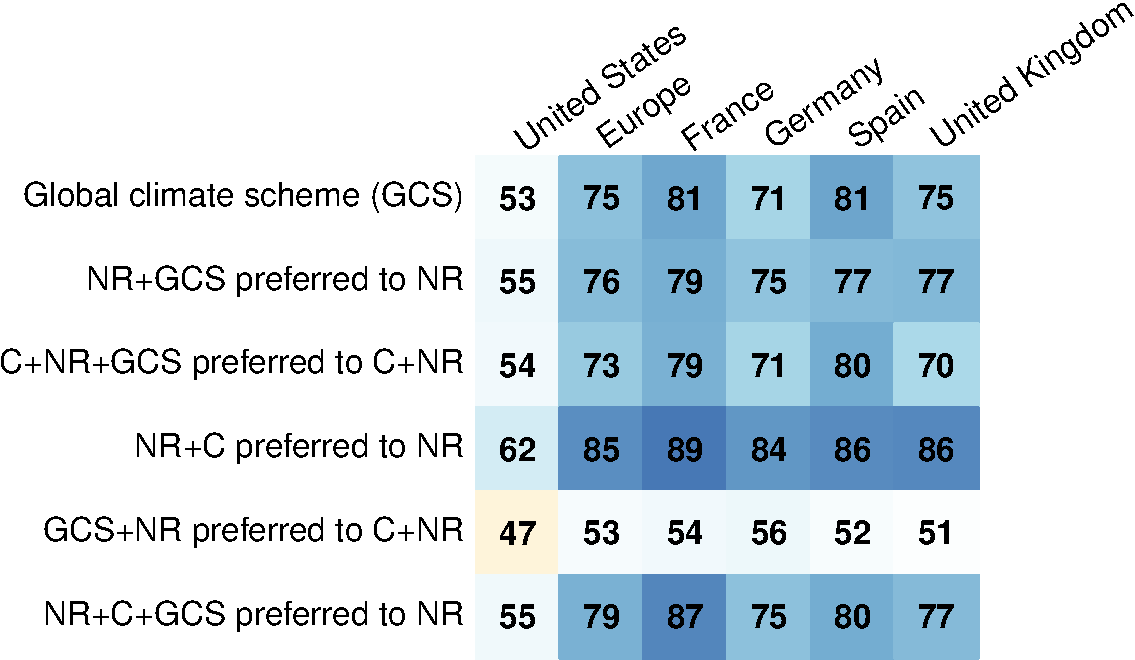
\includegraphics[width=.8\textwidth]{../figures/country_comparison/conjoint_ab_all_positive.pdf}} 
\end{figure}

% \begin{figure}[h!] % already in text
%     \cprotect\caption{[Asked only to non-Republicans] Conjoint analysis n°4: random programs at the Democratic primary. (Question \ref{q:conjoint_r})}\label{fig:ca_r}
%     \makebox[\textwidth][c]{\includegraphics[width=\textwidth]{../figures/country_comparison/ca_r.png}} 
% \end{figure}

% \begin{figure}[h!]
%     \cprotect\caption[Influence of the GCS on preferred platform]{Influence of the GCS on preferred platform:\\ Preference for a random platform A that contains the Global Climate Scheme rather than a platform B that does not (in percent). (Question \ref{q:conjoint_d}; in the U.S., asked only to non-Republicans.)}\label{fig:conjoint_left_ag_b}
%     \makebox[\textwidth][c]{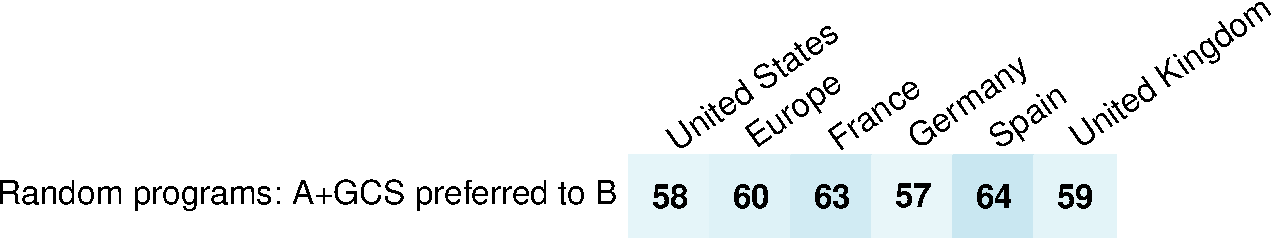
\includegraphics[width=\textwidth]{../figures/country_comparison/conjoint_left_ag_b_binary_positive.pdf}} 
% \end{figure}

\begin{figure}[h] 
  \cprotect\caption[Preferences for various policies in political platforms (original)]{Effects of the presence of a policy (rather than none from this domain) in a random platform on the likelihood that it is preferred to another random platform. Points represent Average Marginal Component Effects and bars 95\% C.I. (\verb|[country]/ca_r|; See English translations in Figure \ref{fig:ca_r}; Question \ref{q:conjoint_r}%; in the U.S., asked only to non-Republicans.
  )}\label{fig:ca_r_en}
    \begin{subfigure}{.97\textwidth}
      \subcaption{Germany}
      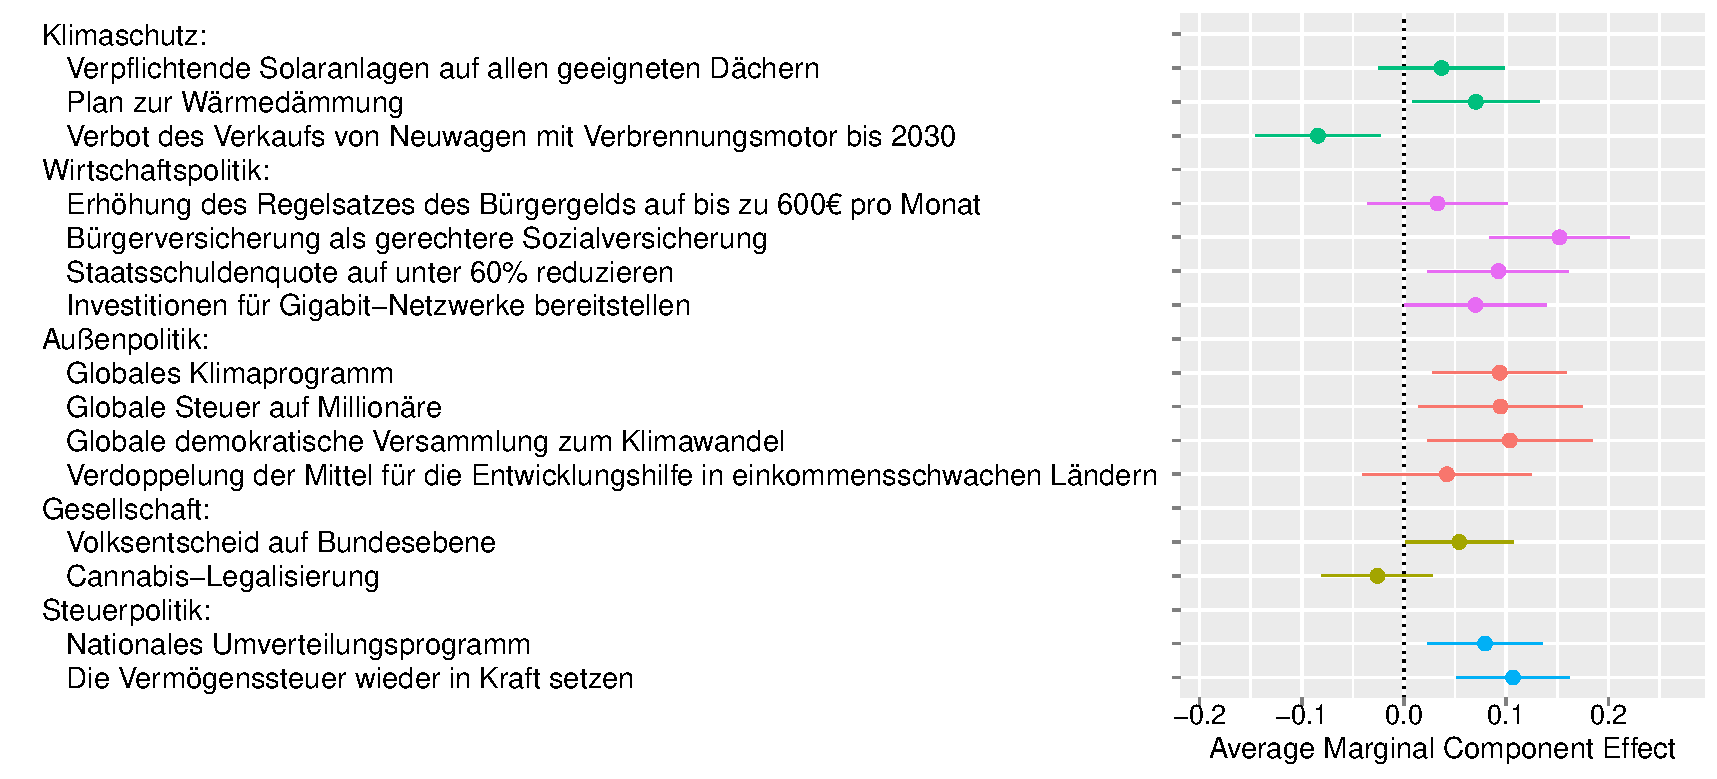
\includegraphics[width=.97\textwidth]{../figures/DE/ca_r.pdf}
    \end{subfigure}
    \begin{subfigure}{.98\textwidth}
      \subcaption{France}
      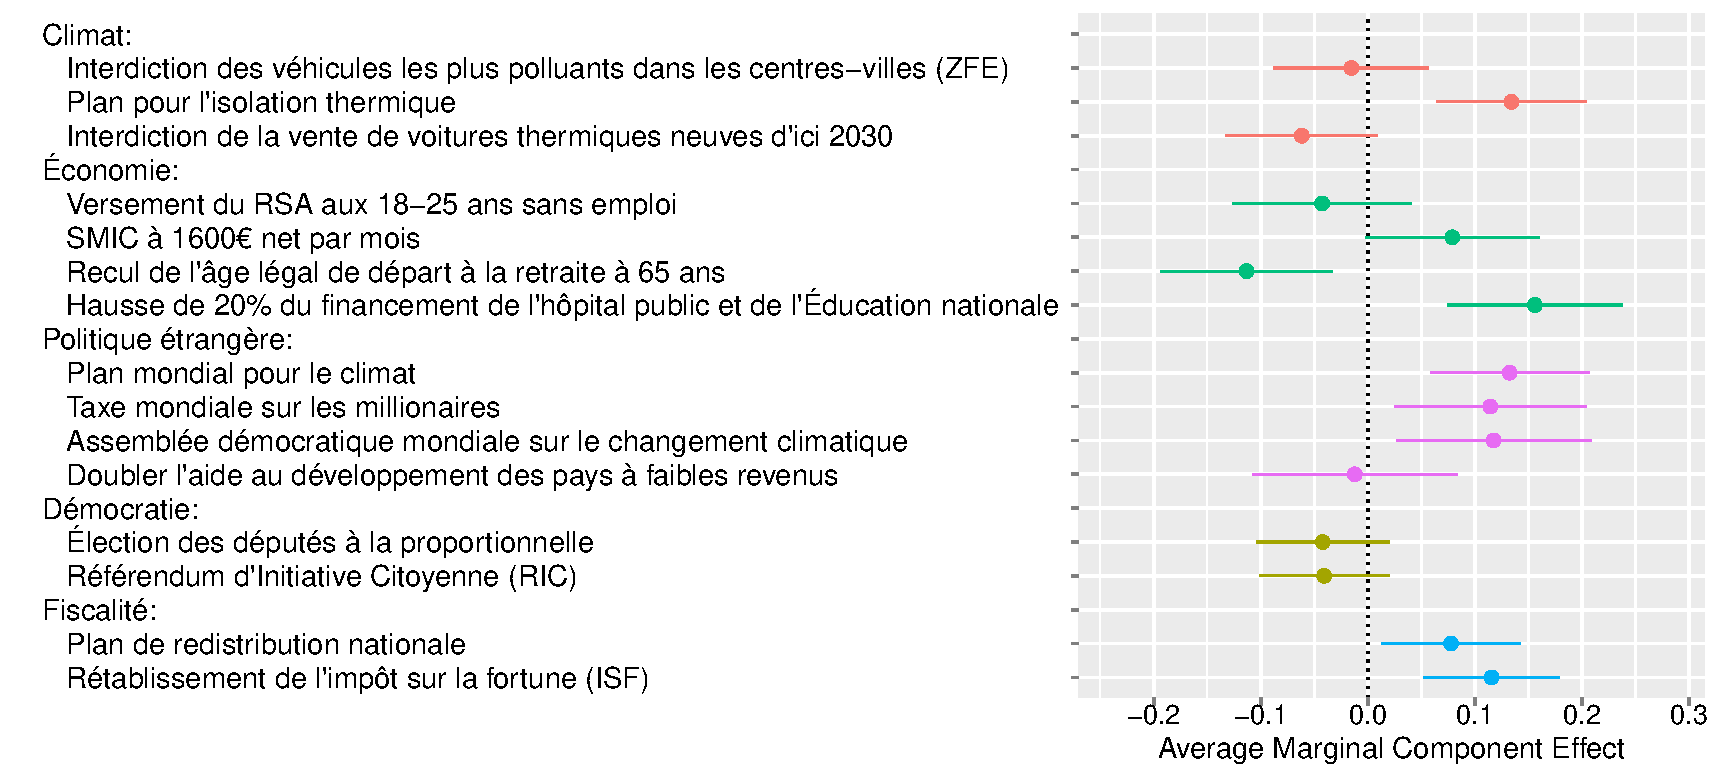
\includegraphics[width=.98\textwidth]{../figures/FR/ca_r.pdf}
    \end{subfigure}
    \begin{subfigure}{.98\textwidth}
      \subcaption{Spain}
      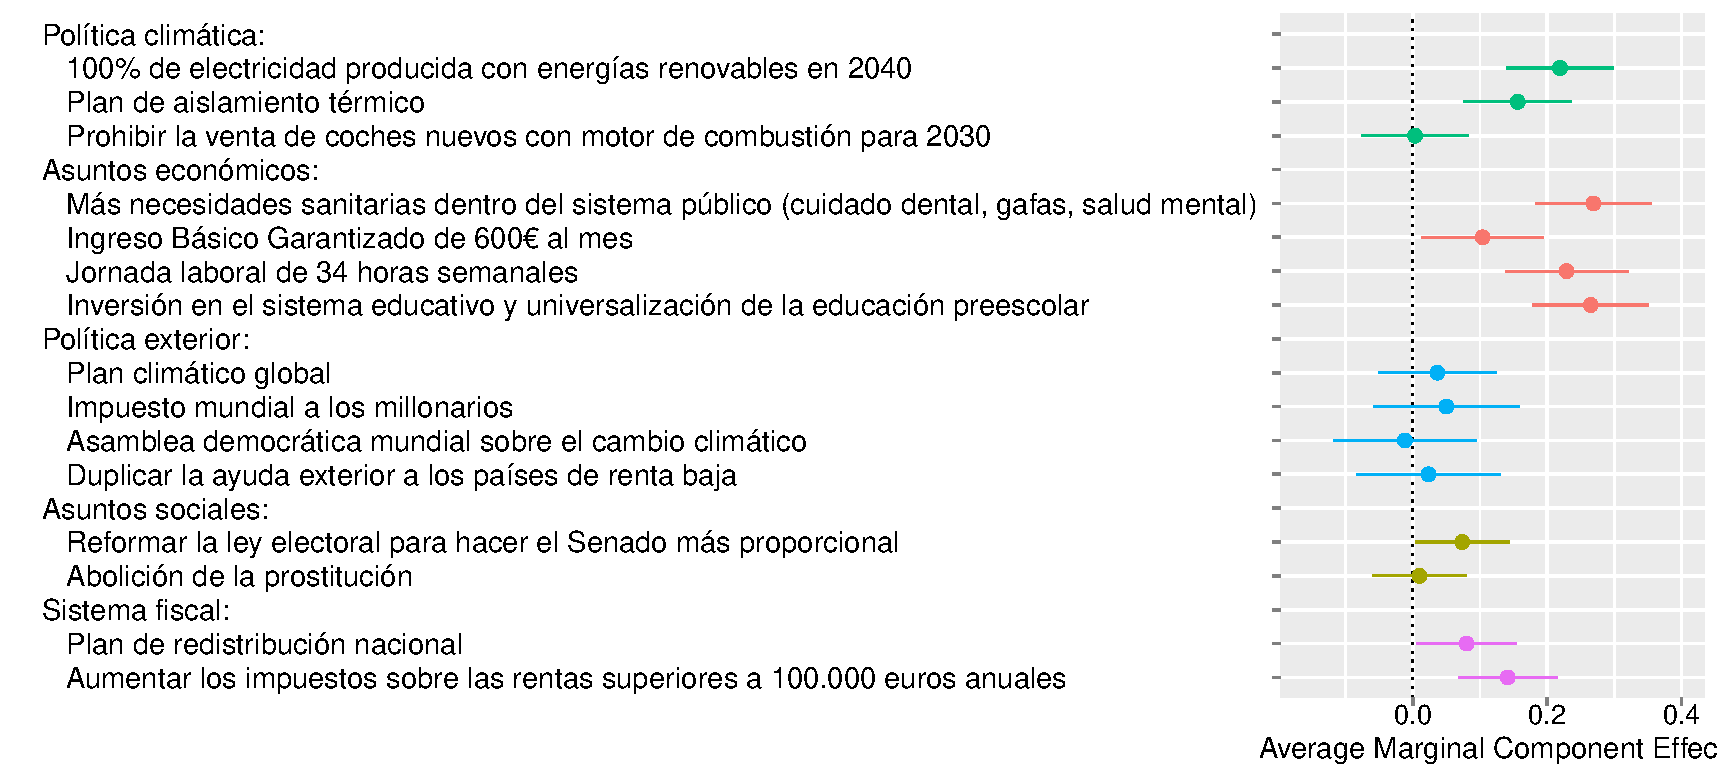
\includegraphics[width=.98\textwidth]{../figures/ES/ca_r.pdf}
    \end{subfigure}
\end{figure}

\begin{figure}[h!]
    \cprotect\caption[Perceptions of the GCS]{Perceptions of the GCS. Elements seen as important for supporting the GCS in a 4-Likert scale (in percent). (\verb|gcs_important_positive|; Question \ref{q:gcs_important})  %\hfill (Back~to~Section~\ref{subsubsec:pros_cons})
    }\label{fig:gcs_important}
    \makebox[\textwidth][c]{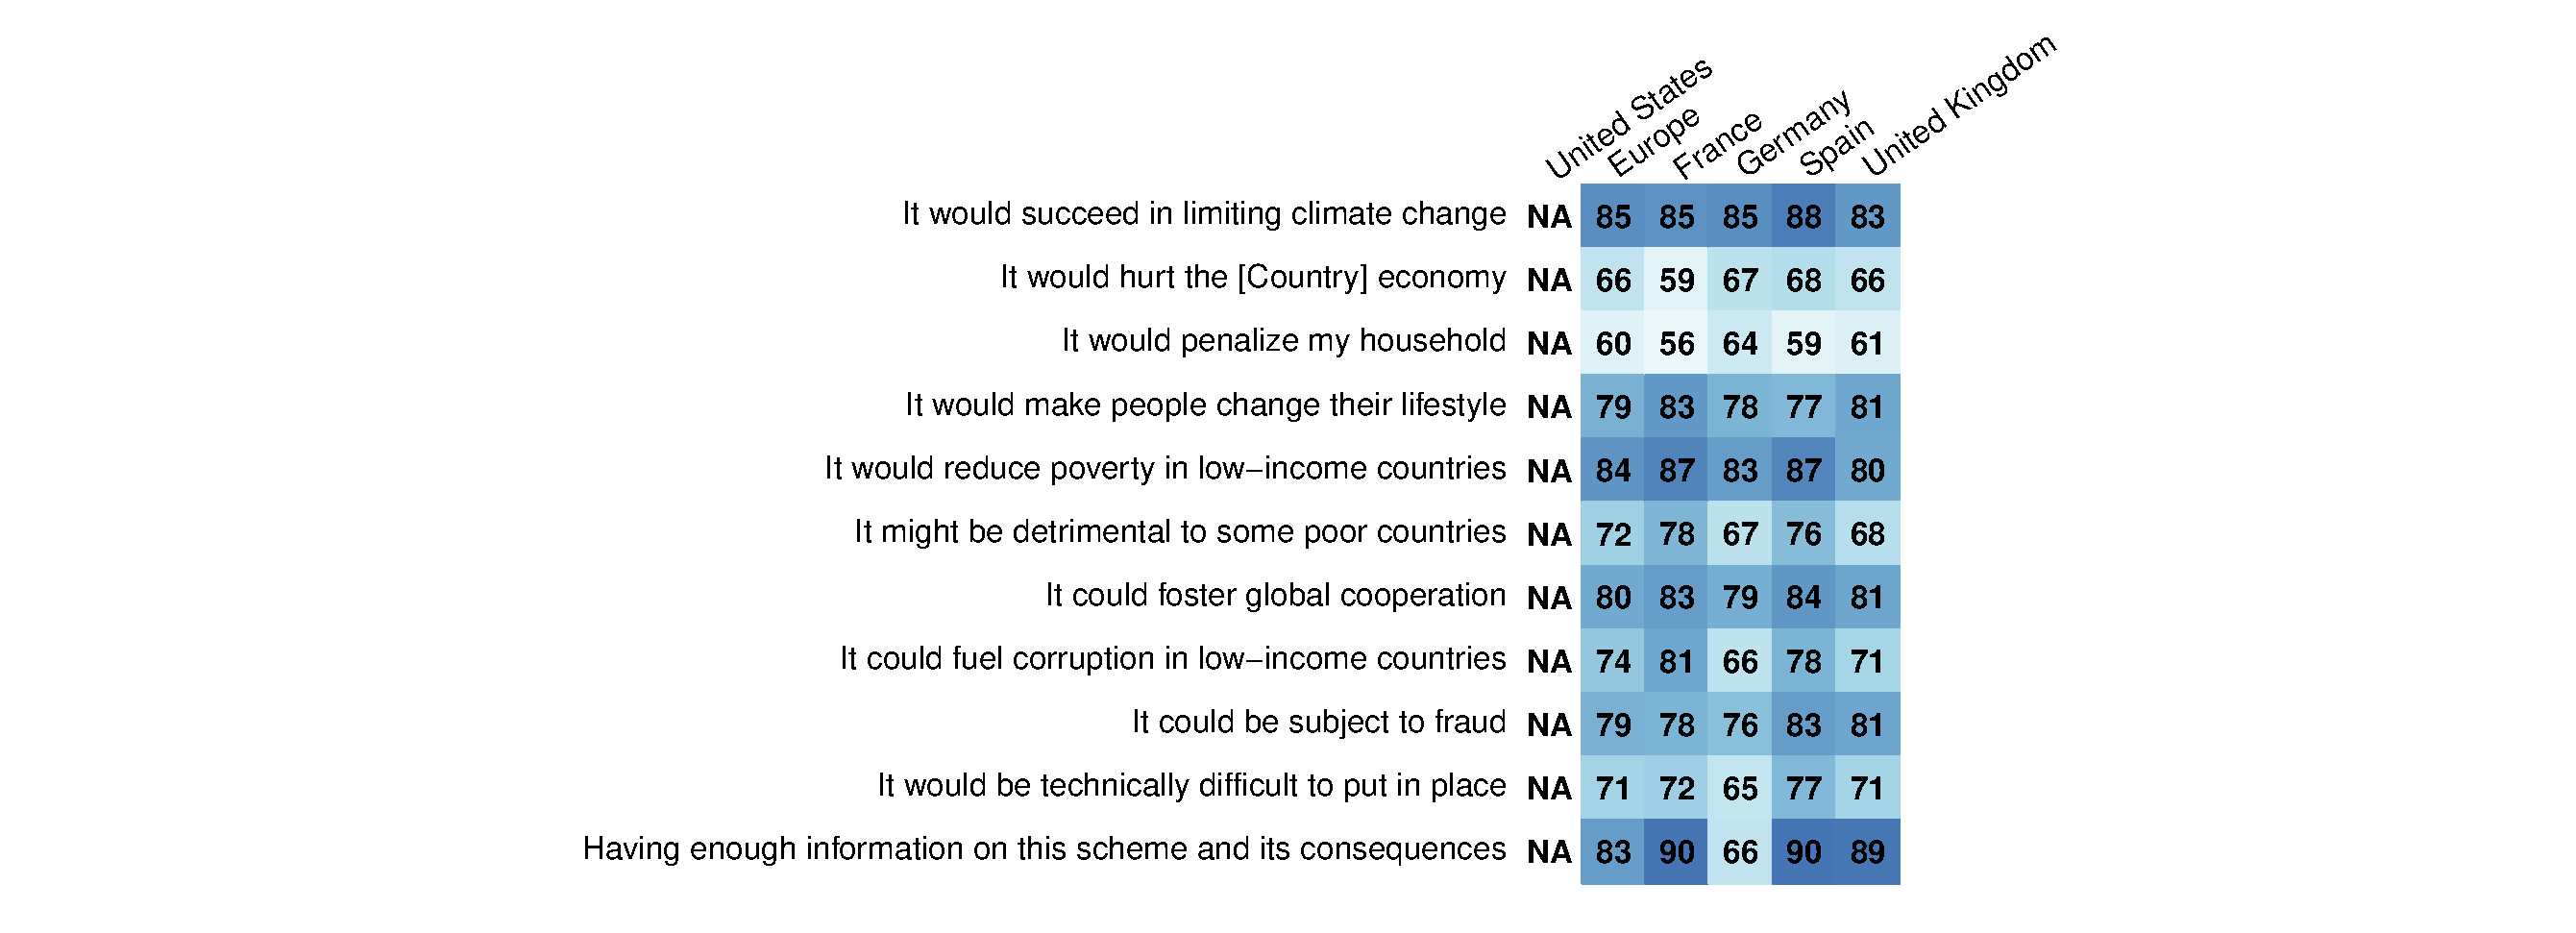
\includegraphics[width=\textwidth]{../figures/country_comparison/gcs_important_positive.pdf}} 
\end{figure}

\begin{figure}[h!]
    \cprotect\caption[Classification of open-ended field on the GCS]{Perceptions of the GCS. Elements found in the open-ended field on the GCS (manually recoded, in percent). \\ ``When thinking about the Global climate scheme, what comes to
    your mind?
    \\ Please list pros and cons of the Global climate scheme.'' (\verb|gcs_field_positive|; Question \ref{q:gcs_field}) %\hfill (Back~to~Section~\ref{subsubsec:pros_cons})
    }\label{fig:gcs_field}
    \makebox[\textwidth][c]{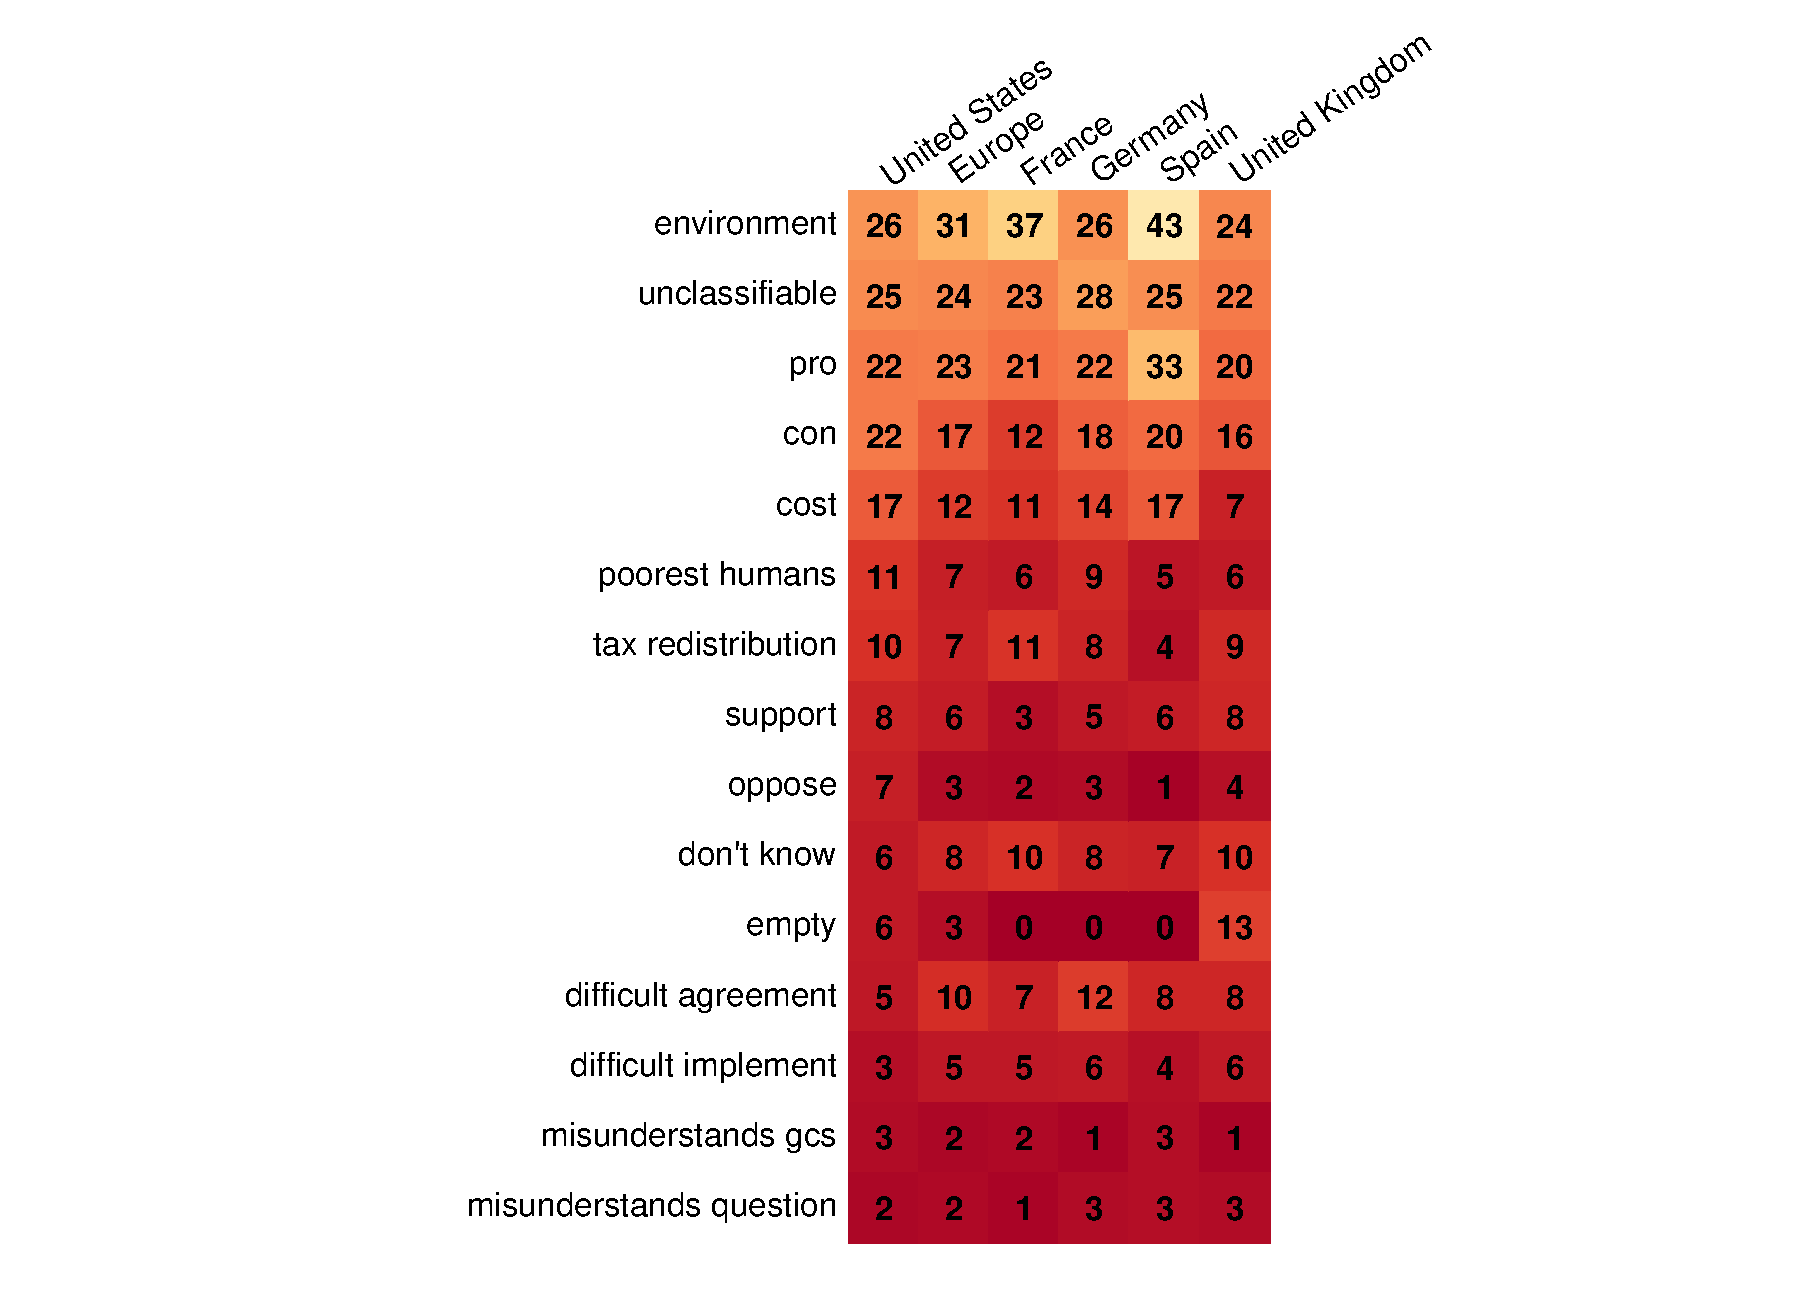
\includegraphics[width=.75\textwidth]{../figures/country_comparison/gcs_field_positive.pdf}} 
\end{figure}

\begin{figure}[h!]
    \cprotect\caption[Topics of open-ended field on the GCS]{Perceptions of the GCS. Keywords found in the open-ended field on the GCS (automatic search ignoring case, in percent). \\ ``When thinking about the Global climate scheme, what comes to
    your mind?
    \\ Please list pros and cons of the Global climate scheme.'' (\verb|gcs_field_contains_positive|; Question \ref{q:gcs_field}) %\hfill (Back~to~Section~\ref{subsubsec:pros_cons})
    }\label{fig:gcs_field_contains}
    \makebox[\textwidth][c]{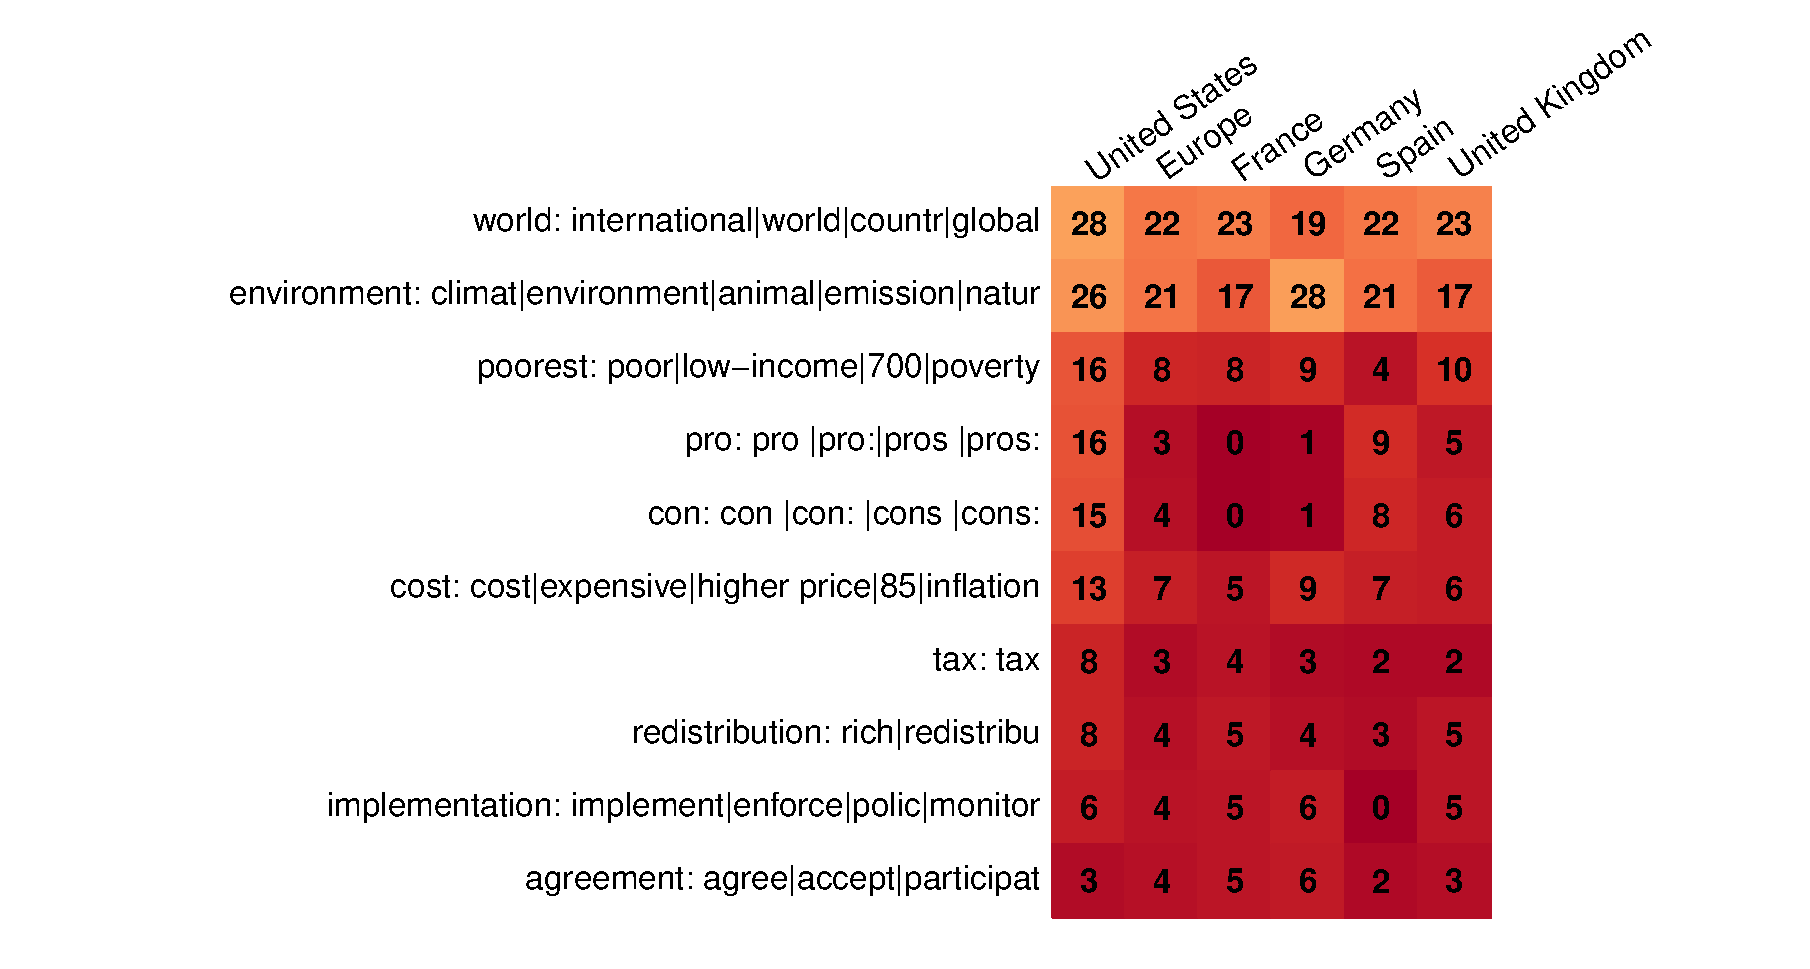
\includegraphics[width=\textwidth]{../figures/country_comparison/gcs_field_contains_positive.pdf}} 
\end{figure}

% \begin{table}[h]
%     \cprotect\caption[Campaign and bandwagon effects on the support for the GCS.]{Effects on the support for the GCS of a question on its pros and cons (either in open-ended of closed format) and on information about the actual support, in the U.S. (See Section \ref{subsec:questionnaire_perceptions} in the \textit{US2} Questionnaire)  \hfill (Back~to~Section~\ref{subsubsec:pros_cons})} \label{tab:branch_gcs}
%     \makebox[\textwidth][c]{
%         
\begin{tabular}{@{\extracolsep{5pt}}lcccc} 
\\[-1.8ex]\hline 
\hline \\[-1.8ex] 
 & \multicolumn{4}{c}{Support} \\ 
\cline{2-5} 
\\[-1.8ex] & \multicolumn{2}{c}{Global Climate Scheme} & \multicolumn{2}{c}{National Redistribution} \\ 
\\[-1.8ex] & (1) & (2) & (3) & (4)\\ 
\hline \\[-1.8ex] 
Control group mean & 0.557 & 0.557 & 0.569 & 0.569  \\ \hline \\[-1.8ex]
 Treatment: Open\mbox{-}ended field on GCS pros \& cons & $-$0.073$^{**}$ & $-$0.071$^{**}$ & $-$0.035 & $-$0.030 \\ 
  & (0.035) & (0.031) & (0.035) & (0.032) \\ 
  Treatment: Closed questions on GCS pros \& cons & $-$0.109$^{***}$ & $-$0.096$^{***}$ & $-$0.065$^{*}$ & $-$0.062$^{**}$ \\ 
  & (0.034) & (0.031) & (0.034) & (0.031) \\ 
  Treatment: Info on actual support for GCS and NR & $-$0.021 & $-$0.015 & 0.048 & 0.056$^{*}$ \\ 
  & (0.034) & (0.031) & (0.033) & (0.031) \\ 
 \hline \\[-1.8ex] 
Includes controls &  & \checkmark &  & \checkmark \\

Observations & 2,000 & 1,995 & 2,000 & 1,995 \\ 
R$^{2}$ & 0.007 & 0.170 & 0.007 & 0.154 \\ 
\hline 
\hline \\[-1.8ex] 
\end{tabular} 
%     }
%     {\footnotesize %\textit{Note}: 
%     }
% \end{table}

\begin{figure}[h!]
    \cprotect\caption[Donation to Africa vs. own country]{Donation in case of lottery win, depending on the recipient's (randomly drawn) nationality (mean). (\verb|donation_mean|; Question \ref{q:donation})%\hfill (Back~to~Section~\ref{subsec:universalistic})
    }\label{fig:donation}
    \makebox[\textwidth][c]{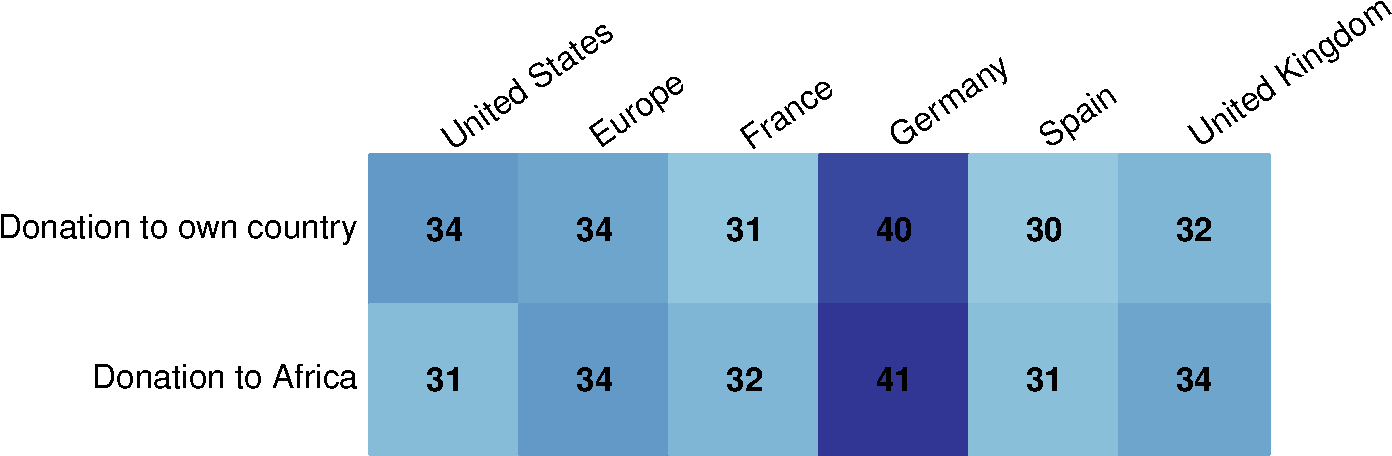
\includegraphics[width=.8\textwidth]{../figures/country_comparison/donation_mean.pdf}} 
\end{figure}

% \begin{table}[h]
%     \cprotect\caption[Donation to Africa vs. own country]{Donation in case of lottery win, depending on the recipient's (randomly drawn) nationality. (Question \ref{q:donation})\hfill (Back~to~Section~\ref{subsec:universalistic})} \label{tab:donation}
%     \makebox[\textwidth][c]{
\begin{tabular}{@{\extracolsep{5pt}}lcccc} 
\\[-1.8ex]\hline 
\hline \\[-1.8ex] 
 & \multicolumn{4}{c}{Donation to poor people (in \%)} \\ 
\cline{2-5} 
\\[-1.8ex] & All & US & US & Eu \\ 
\hline \\[-1.8ex] 
 Poor is in own country & 0.590 & 2.509$^{**}$ & 0.046 & $-$1.349 \\ 
  & (0.799) & (1.152) & (1.691) & (1.108) \\ 
  Poor is in own country $\times$ Vote: \textit{not} Biden &  &  & 3.954$^{*}$ &  \\ 
  &  &  & (2.279) &  \\ 
 \hline \\[-1.8ex] 
Mean & 34.034 & 33.658 & 33.658 & 34.41 \\ 
Observations & 6,000 & 3,000 & 3,000 & 3,000 \\ 
R$^{2}$ & 0.0001 & 0.002 & 0.034 & 0.0005 \\ 
\hline 
\hline \\[-1.8ex] 
\end{tabular} }
% \end{table}

\begin{figure}[h!]
    \cprotect\caption[Support for a national wealth tax]{Support for a national wealth tax. \\ ``Do you support or oppose a tax on millionaires in [the U.S.] to finance [\textit{US2}: affordable housing and universal childcare/pre-K; \textit{Eu}: finance government hospitals and schools]?'' %financing public services like healthcare, education, and social housing. 
    (\verb|national_tax_support|; Question \ref{q:national_tax})}\label{fig:national_tax}
    \makebox[\textwidth][c]{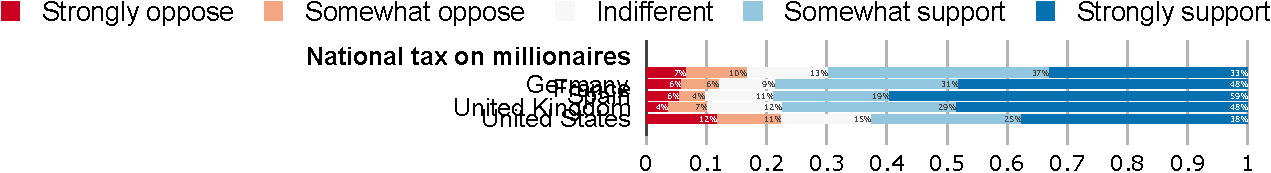
\includegraphics[width=\textwidth]{../figures/country_comparison/national_tax_support.pdf}} 
\end{figure}

\begin{figure}[h!]
    \cprotect\caption[Support for a global wealth tax]{Support for a global wealth tax. \\
    ``Do you support or oppose a tax on millionaires of all countries to finance low-income countries? \\
    Such tax would finance infrastructure and public services such as access to drinking water, healthcare, and education.'' (\verb|global_tax_support|; Question \ref{q:global_tax})}\label{fig:global_tax}
    \makebox[\textwidth][c]{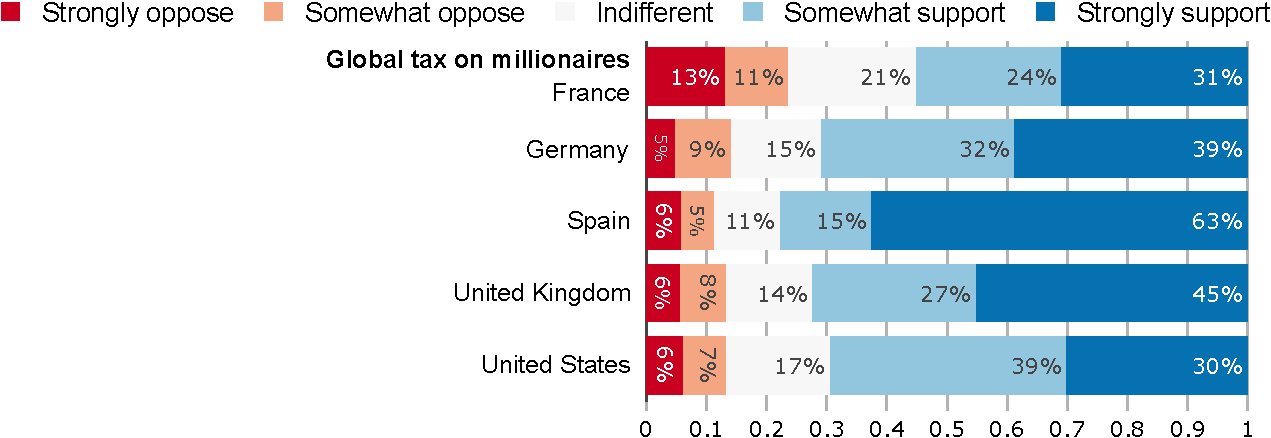
\includegraphics[width=\textwidth]{../figures/country_comparison/global_tax_support.pdf}} 
\end{figure}

\begin{figure}[h!]
    \cprotect\caption[Preferred share of global tax for low-income countries]{Preferred share of global wealth tax revenues that should be pooled to finance low-income countries. (\verb|global_tax_global_share|; Question \ref{q:global_tax_global_share})}\label{fig:global_tax_global_share}
    \makebox[\textwidth][c]{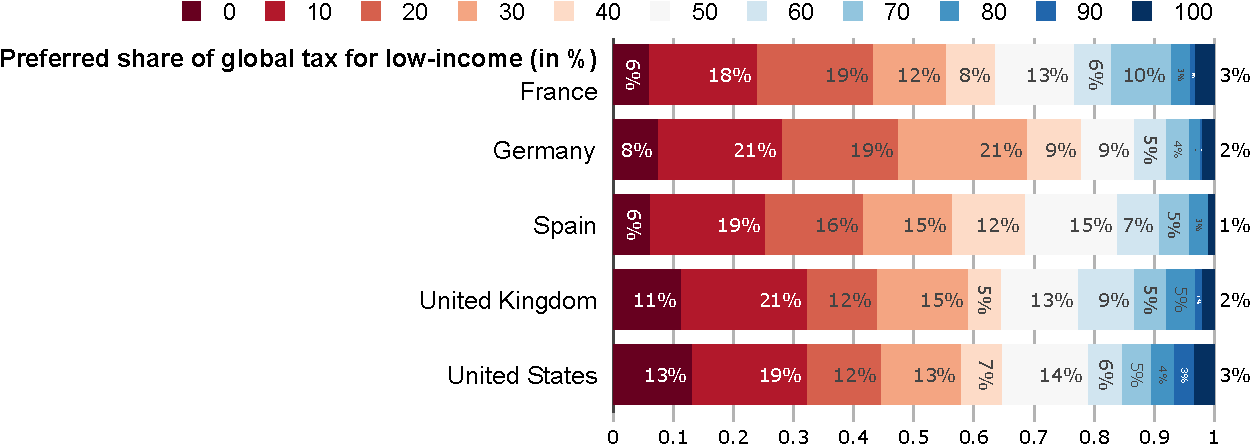
\includegraphics[width=\textwidth]{../figures/country_comparison/global_tax_global_share.pdf}} 
\end{figure}

\begin{figure}[h!]
    \cprotect\caption[Support for sharing half of global tax revenues with low-income countries]{Support for sharing half of global tax revenues with low-income countries, rather that each country retaining all the revenues it collects (in percent). (\verb|global_tax_sharing_positive|; Question \ref{q:global_tax_sharing})}\label{fig:global_tax_sharing}
    \makebox[\textwidth][c]{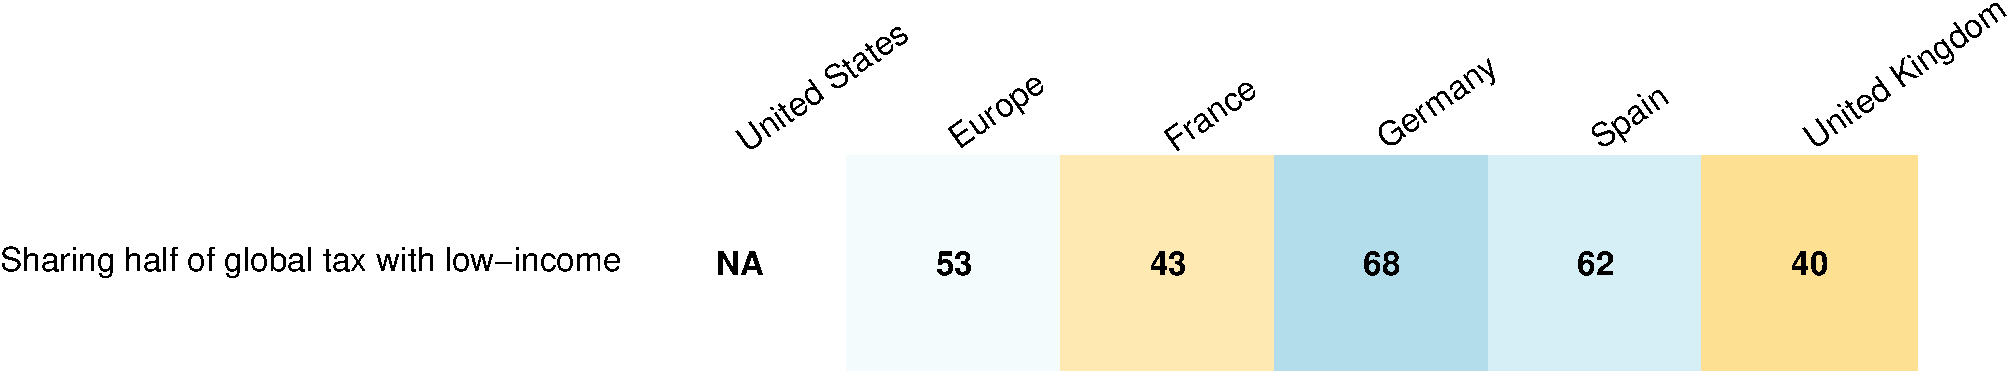
\includegraphics[width=\textwidth]{../figures/country_comparison/global_tax_sharing_positive.pdf}} 
\end{figure}

% \begin{figure}
%     \centering 
%     \cprotect\caption{Your previous answer shows that you would like to increase [UK] foreign aid.\\How would you like to finance such increase in foreign aid? (Multiple answers possible)}
%     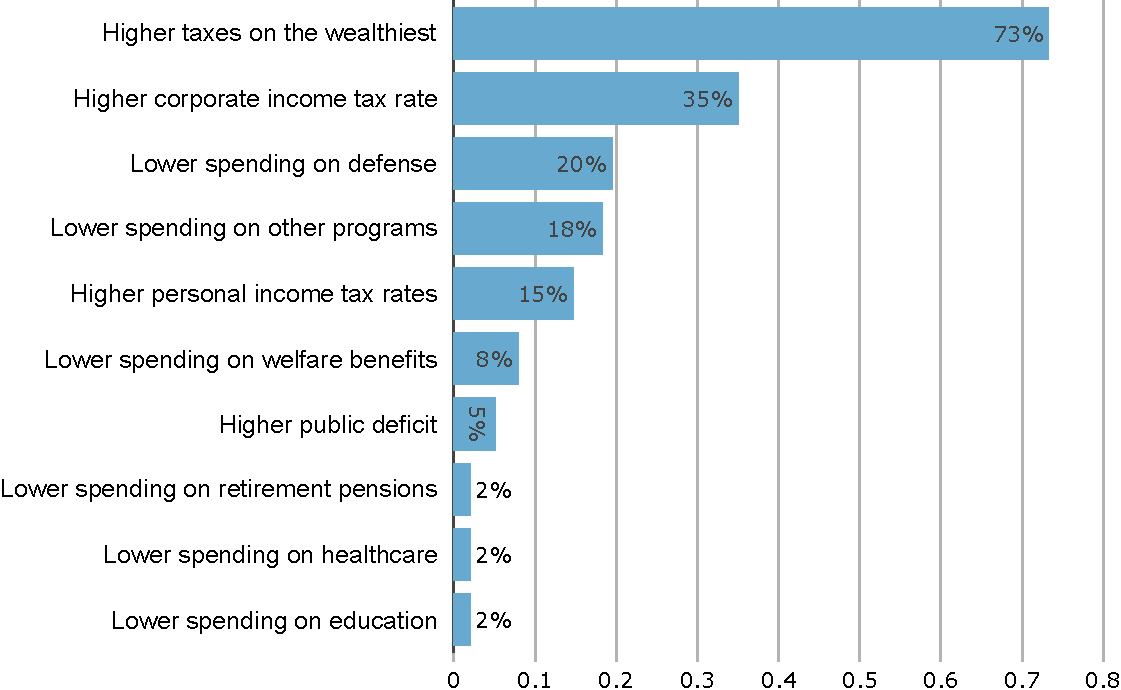
\includegraphics[width=\columnwidth]{../figures/all/foreign_aid_raise.pdf} 
% \end{figure}		
% \begin{figure}
%     \centering 
%     \cprotect\caption{Your previous answer shows that you would like to reduce [UK] foreign aid.\\How would you like to use the freed budget? (Multiple answers possible)}
%     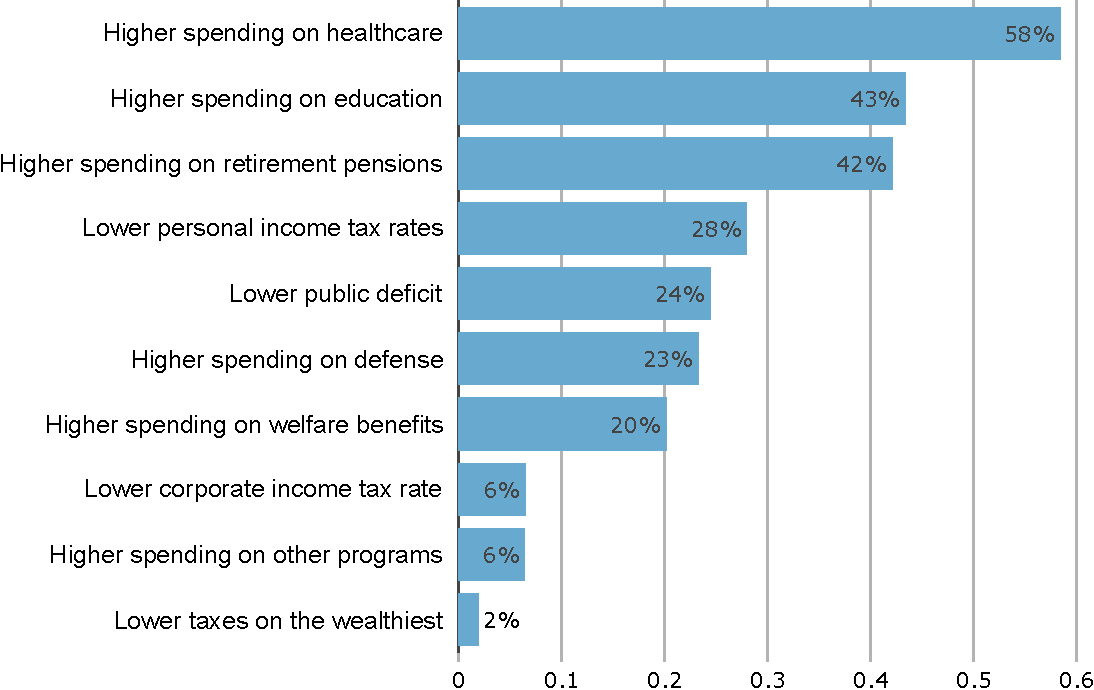
\includegraphics[width=\columnwidth]{../figures/all/foreign_aid_reduce.pdf} 
% \end{figure}

\begin{figure}[h!]
    \cprotect\caption[Perceived foreign aid]{Perceived foreign aid. ``From your best guess, what percentage of [own country] government spending is allocated to foreign aid (that is, to reduce poverty in low-income countries)?'' (\verb|foreign_aid_belief_agg|; Question \ref{q:foreign_aid_belief})  %\hfill (Back~to~Section~\ref{subsubsec:support_foreign_aid}) 
    \\ Actual values: France: 0.8\%; Germany: 1.3\%; Spain: 0.5\%; UK: 1.7\%; U.S.: 0.4\%.}\label{fig:foreign_aid_belief}
    \makebox[\textwidth][c]{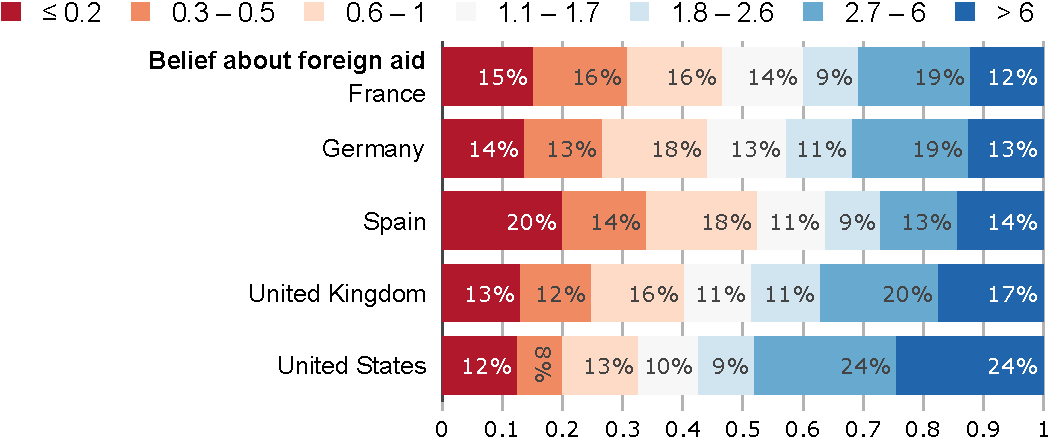
\includegraphics[width=\textwidth]{../figures/country_comparison/foreign_aid_belief_agg.pdf}} 
\end{figure}

\begin{figure}[h!]
    \cprotect\caption[Preferred foreign aid (without info on actual amount)]{Preferred foreign aid (without info on actual amount). \\ ``If you could choose the government spending, what percentage would you allocate
    to foreign aid?'' (\verb|foreign_aid_preferred_no_info_agg|; Question \ref{q:foreign_aid_preferred})  %\hfill (Back~to~Section~\ref{subsubsec:support_foreign_aid})
    }\label{fig:foreign_aid_preferred_no_info}
    \makebox[\textwidth][c]{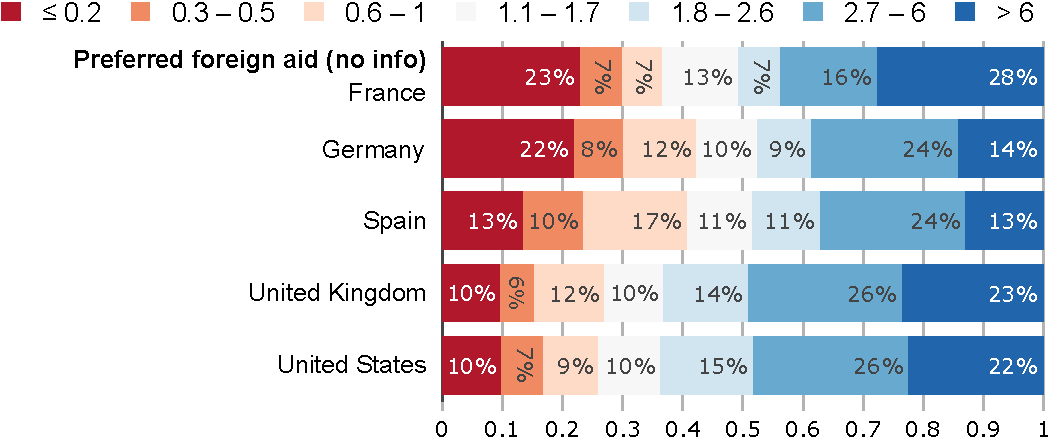
\includegraphics[width=\textwidth]{../figures/country_comparison/foreign_aid_preferred_no_info_agg.pdf}} 
\end{figure}

\begin{figure}[h!]
    \cprotect\caption[Preferred foreign aid (after info on actual amount)]{Preferred foreign aid (after info on actual amount). \\ ``Actually,
    [US1: 0.4\%; FR: 0.8\%; DE: 1.3\%; ES: 0.5\%; UK: 1.7\%] of [own country] government spending is allocated to foreign aid. \\
    If you could choose the government spending, what percentage would you allocate
    to foreign aid?'' (\verb|foreign_aid_preferred_info_agg|; Question \ref{q:foreign_aid_preferred})  %\hfill (Back~to~Section~\ref{subsubsec:support_foreign_aid})
    }\label{fig:foreign_aid_preferred_info}
    \makebox[\textwidth][c]{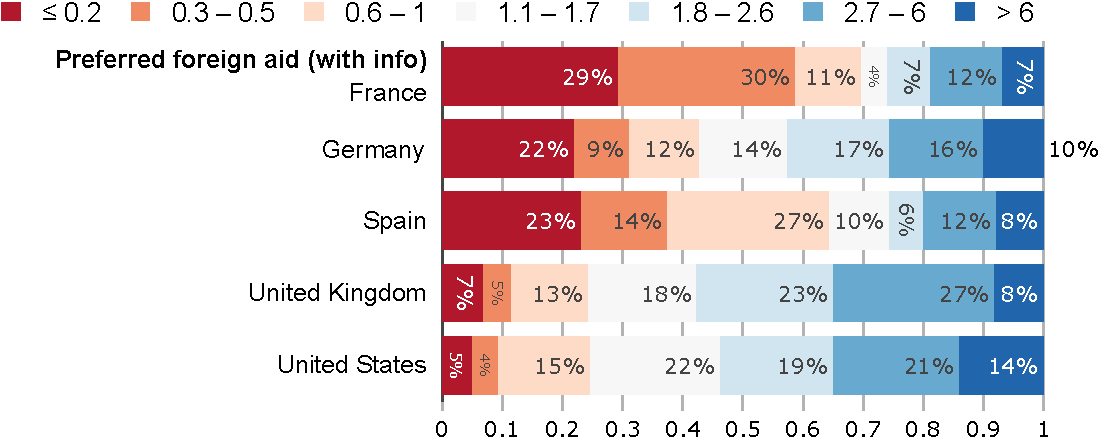
\includegraphics[width=\textwidth]{../figures/country_comparison/foreign_aid_preferred_info_agg.pdf}} 
\end{figure}

\begin{figure} 
    \cprotect\caption[Actual, perceived and preferred amount of foreign aid (mean)]{Actual, perceived and preferred amount of foreign aid, with random info (or not) on actual amount. (\textit{Mean} in percent of public spending; \verb|foreign_aid_amount_mean|; Questions \ref{q:foreign_aid_belief}, \ref{q:foreign_aid_preferred})  %\hfill (Back~to~Section~\ref{subsubsec:support_foreign_aid})
    }\label{fig:foreign_aid_amount}
    \makebox[\textwidth][c]{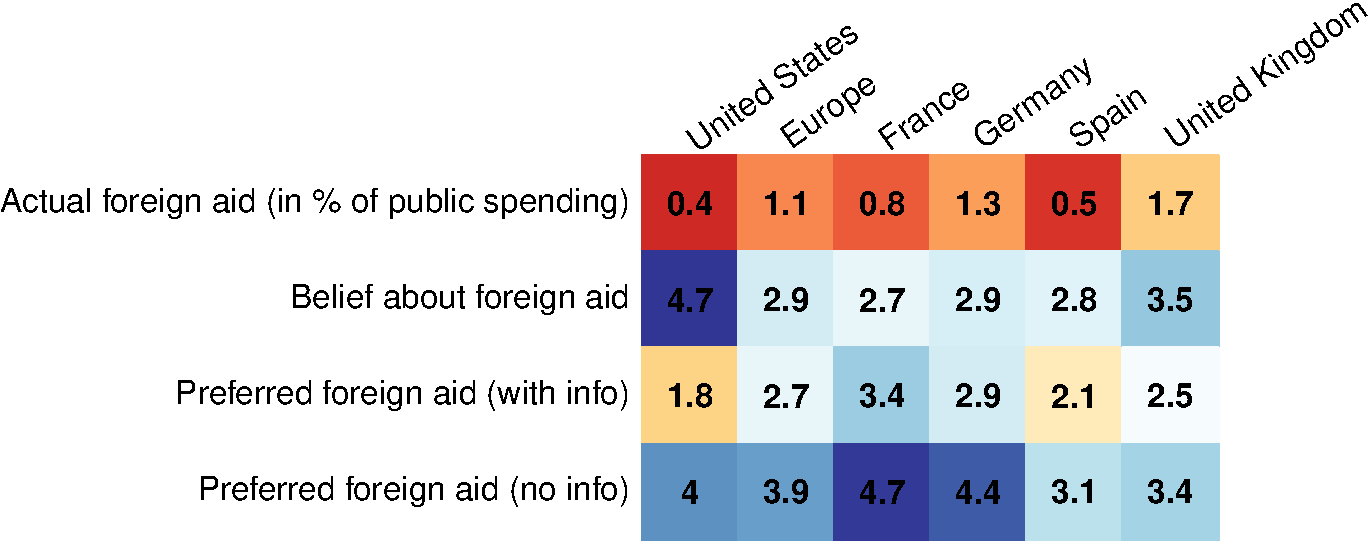
\includegraphics[width=.9\textwidth]{../figures/country_comparison/foreign_aid_amount_mean.pdf} } 
\end{figure}

% \begin{figure} 
%     \cprotect\caption{Actual, perceived and preferred amount of foreign aid, with random info (or not) on actual amount. (\textit{Median}, Questions \ref{q:foreign_aid_belief}, \ref{q:foreign_aid_preferred})}\label{fig:foreign_aid_amount}
%     \makebox[\textwidth][c]{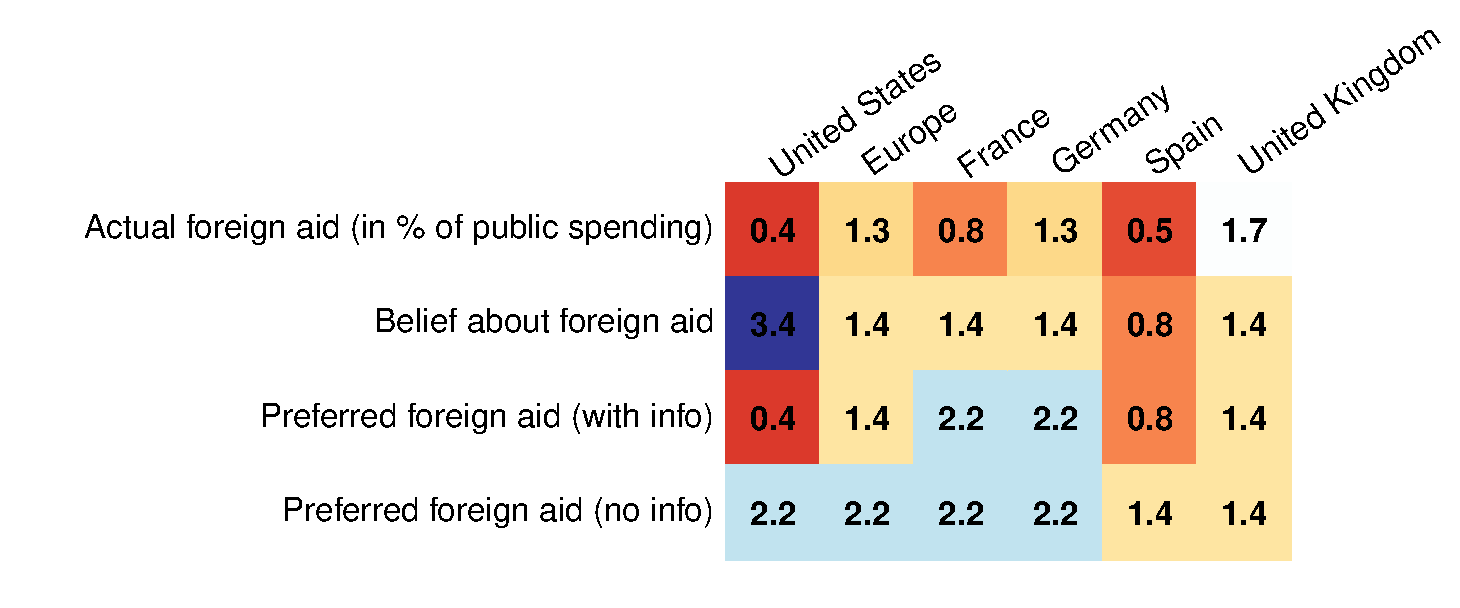
\includegraphics[width=.9\textwidth]{../figures/country_comparison/foreign_aid_amount_median.pdf} } % TODO? add? not necessary as the info on median can be deduced from below figures
% \end{figure}

\begin{figure} 
    % \cprotect\caption{Support for increased foreign aid (vs. reduced or stable): from previous question, and directly asked (with info).}\vspace{-.2cm}
    % 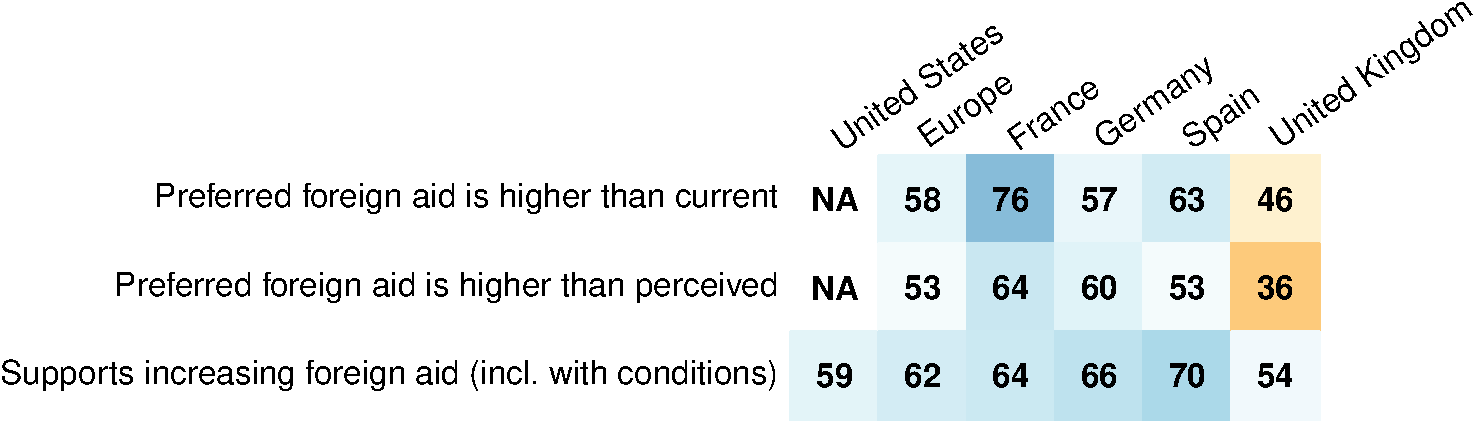
\includegraphics[height=.32\textheight]{../figures/country_comparison/foreign_aid_more_positive.pdf} 
    \cprotect\caption[Preferred foreign aid (summary)]{Preferred foreign aid (after info or after perception). (\verb|foreign_aid_no_less_all_positive|; Questions \ref{q:foreign_aid_belief} and \ref{q:foreign_aid_preferred})}\label{fig:foreign_aid_no_less_all}
    \makebox[\textwidth][c]{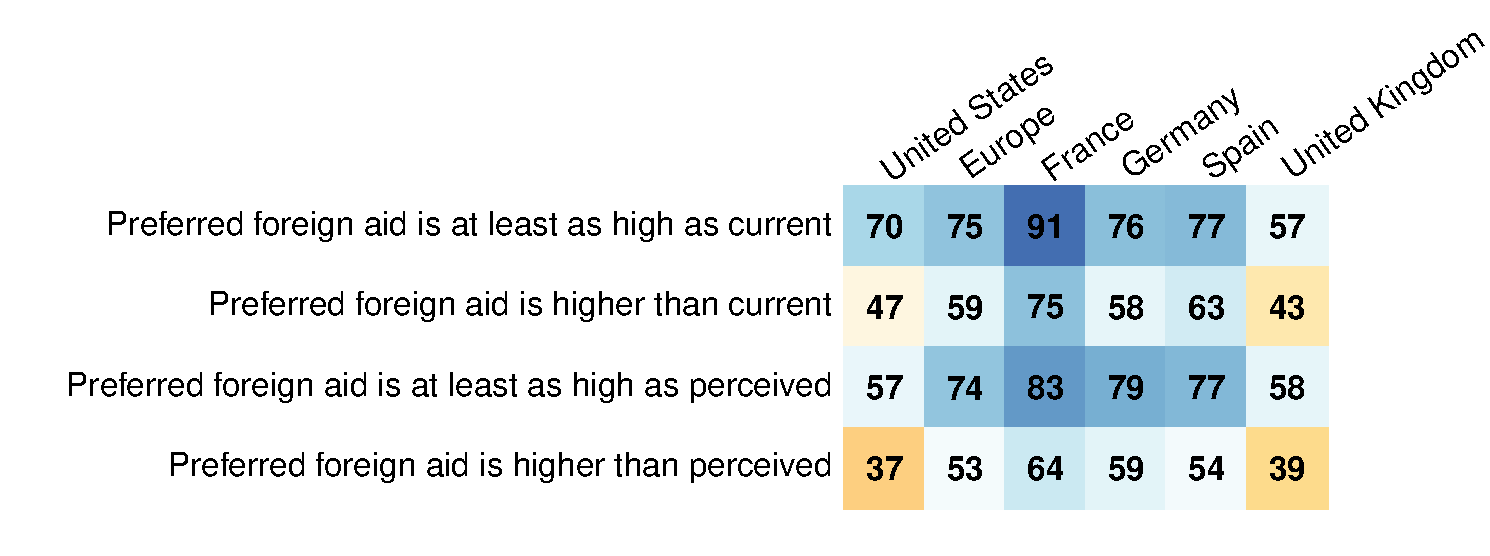
\includegraphics[width=\textwidth]{../figures/country_comparison/foreign_aid_no_less_all_positive.pdf} }
\end{figure} 

\begin{figure}[h!]
    \cprotect\caption[Preferences for funding increased foreign aid]{Preferences for funding increased foreign aid. [Asked iff preferred foreign aid is strictly greater than [Info: actual; No info: perceived] foreign aid] \\ ``How would you like to finance such increase in foreign aid? (Multiple answers possible)'' (in percent) (\verb|foreign_aid_raise_positive|; Question \ref{q:foreign_aid_raise_how})  %\hfill (Back~to~Section~\ref{subsubsec:support_foreign_aid})
    }\label{fig:foreign_aid_raise_how}
    \makebox[\textwidth][c]{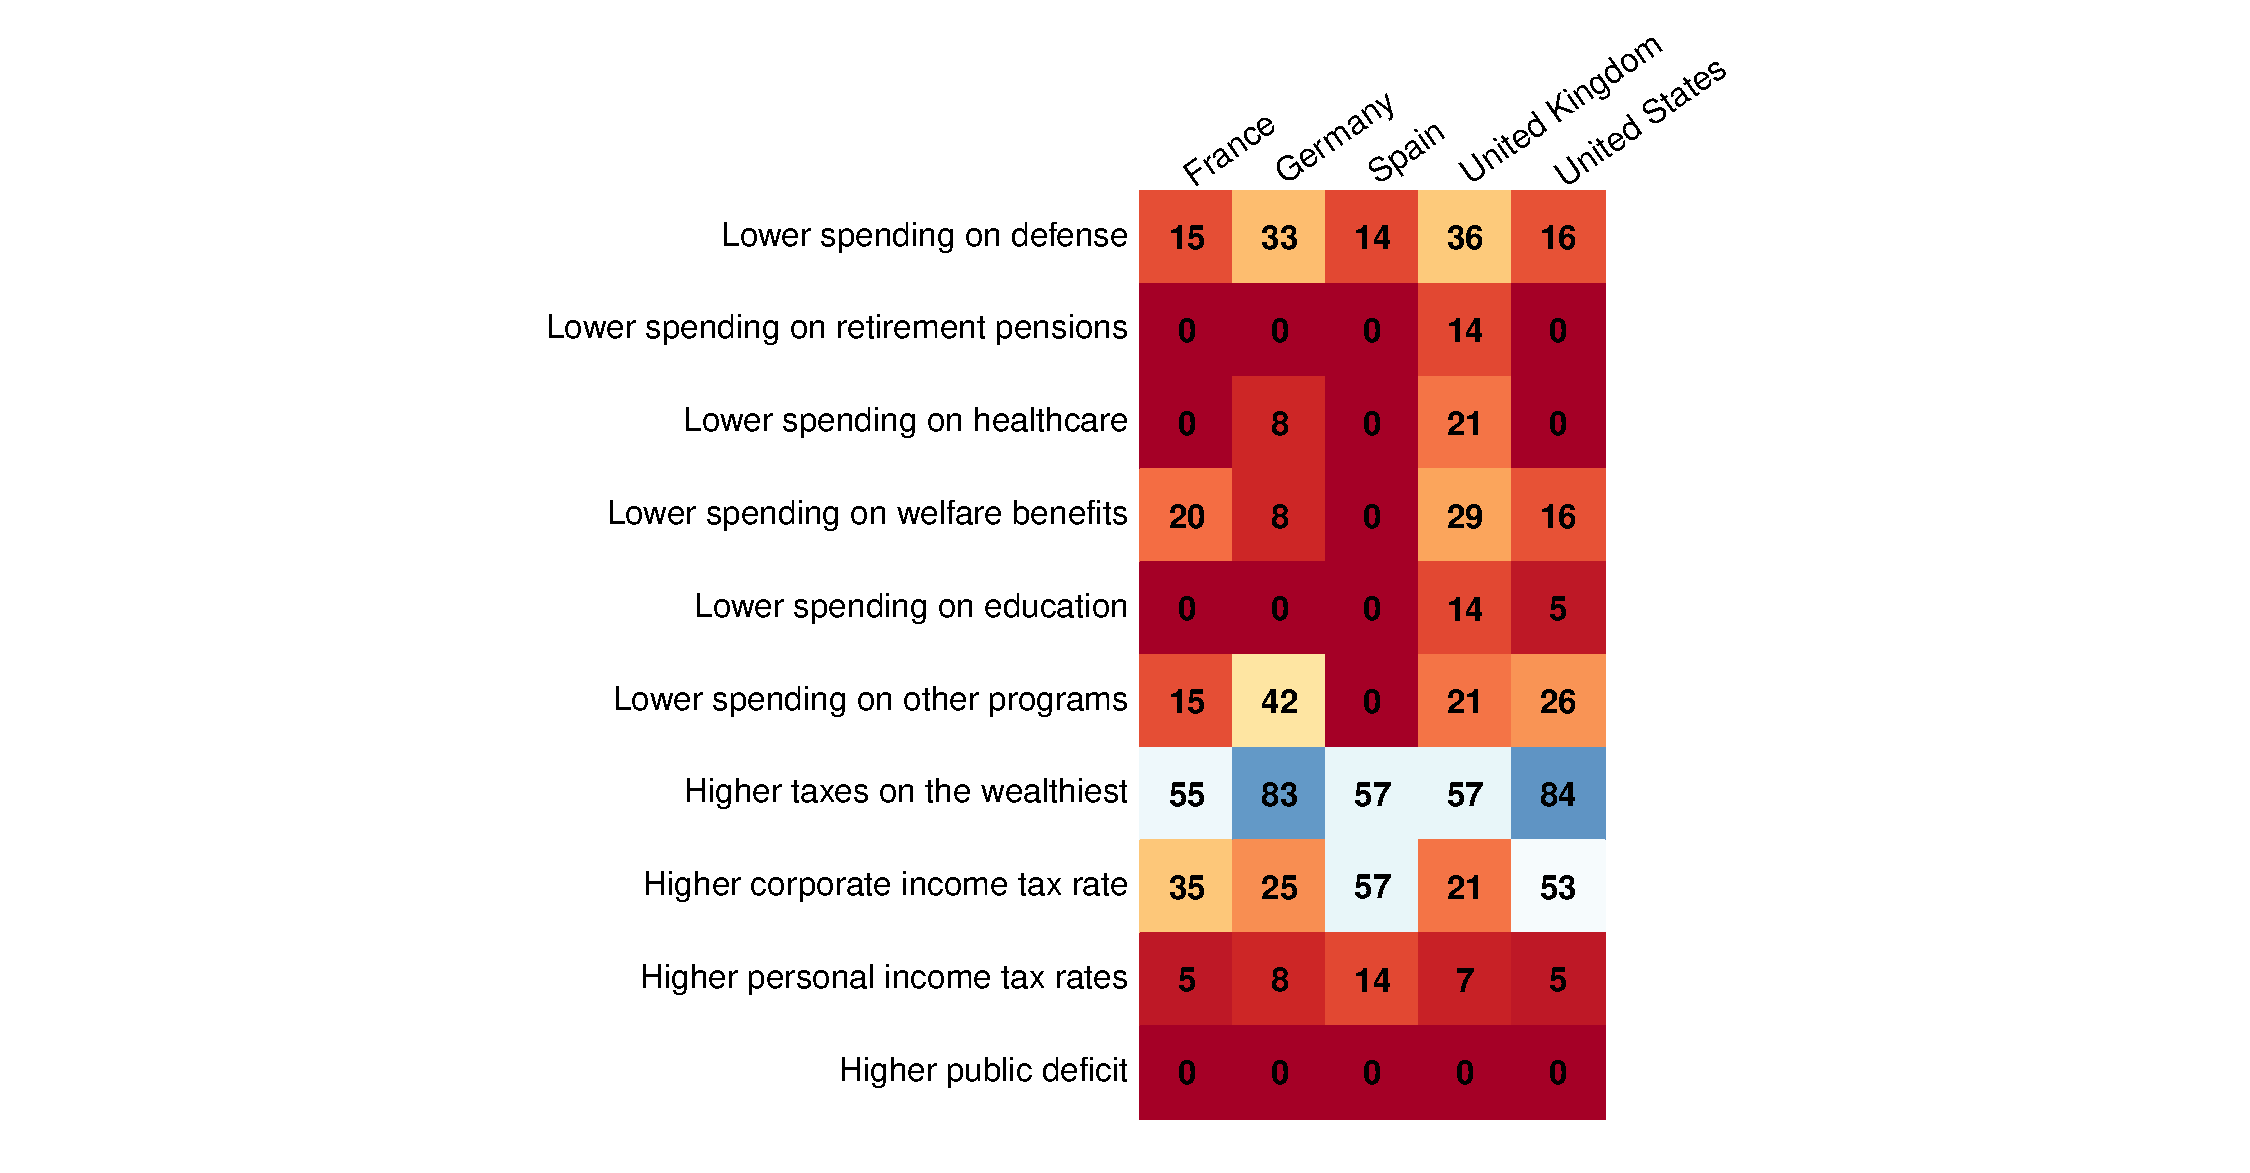
\includegraphics[width=.75\textwidth]{../figures/country_comparison/foreign_aid_raise_positive.pdf}} 
\end{figure}

\begin{figure}[h!]
    \cprotect\caption[Preferences of spending following reduced foreign aid]{Preferences of spending following reduced foreign aid. [Asked iff preferred foreign aid is strictly lower than [Info: actual; No info: perceived] foreign aid] \\ ``How would you like to use the freed budget? (Multiple answers possible)'' (in percent) (\verb|foreign_aid_reduce_positive|; Question \ref{q:foreign_aid_reduce_how})  %\hfill (Back~to~Section~\ref{subsubsec:support_foreign_aid})
    }\label{fig:foreign_aid_reduce_how}
    \makebox[\textwidth][c]{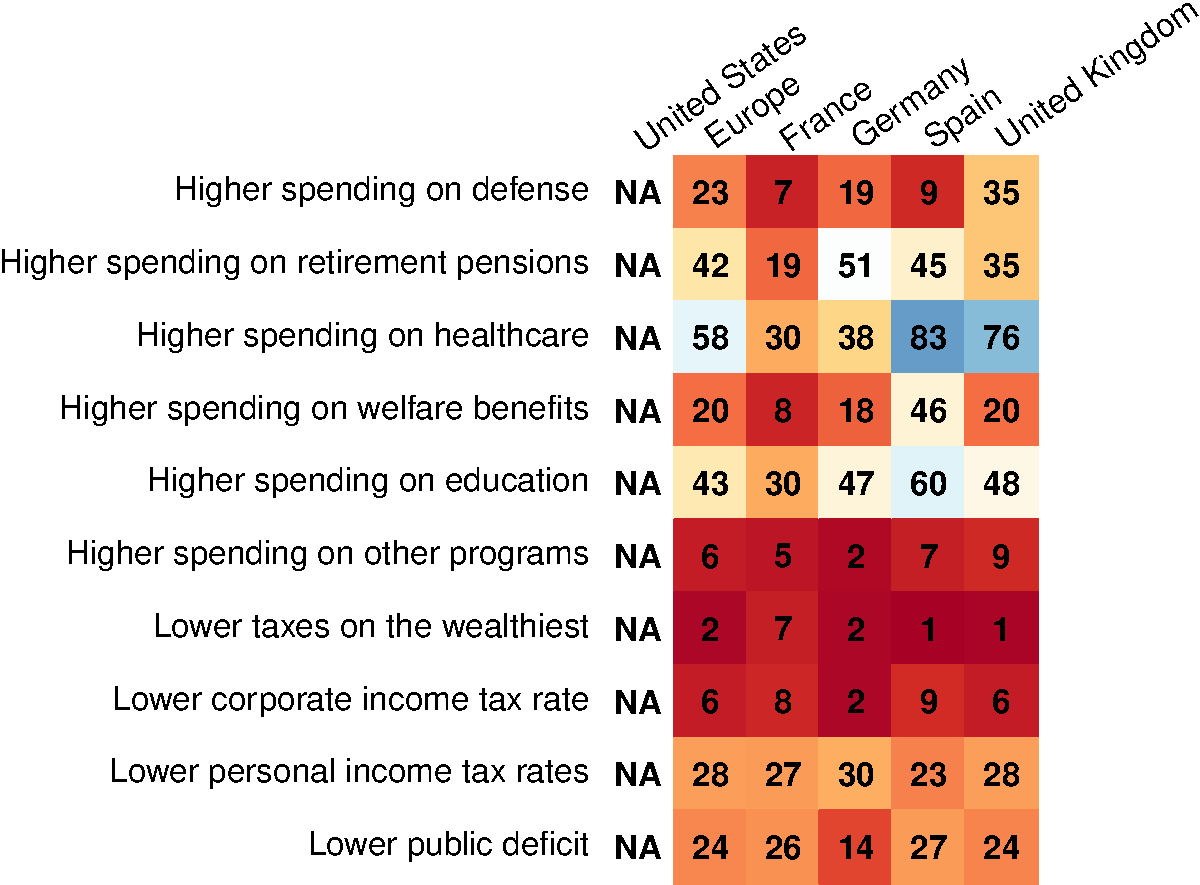
\includegraphics[width=.75\textwidth]{../figures/country_comparison/foreign_aid_reduce_positive.pdf}} 
\end{figure}

% \begin{figure}[h!]
%     \cprotect\caption[Attitudes on the evolution of foreign aid]{Attitudes regarding the evolution of [own country] foreign aid. (Question \ref{q:foreign_aid_raise_support})}\label{fig:foreign_aid_raise_support}
%     \makebox[\textwidth][c]{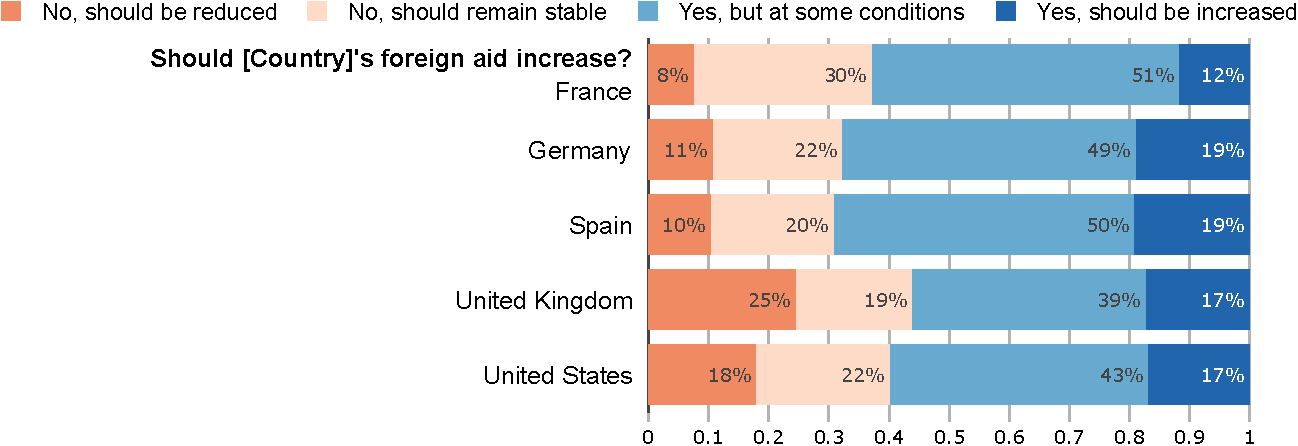
\includegraphics[width=\textwidth]{../figures/country_comparison/foreign_aid_raise_support.pdf}} 
% \end{figure}

% \begin{figure}[h!]
%     \cprotect\caption[Conditions at which foreign aid should be increased]{Conditions at which foreign aid should be increased (in percent). [Asked to those who wish an increase of foreign aid at some conditions.] (Question \ref{q:foreign_aid_condition})}\label{fig:foreign_aid_condition}
%     \makebox[\textwidth][c]{\includegraphics[width=\textwidth]{../figures/country_comparison/foreign_aid_condition_positive.pdf}} 
% \end{figure}

% \begin{figure}[h!]
%     \cprotect\caption[Reasons why foreign aid should not be increased]{Reasons why foreign aid should not be increased (in percent). [Asked to those who wish a decrease or stability of foreign aid.] (Question \ref{q:foreign_aid_no})}\label{fig:foreign_aid_no}
%     \makebox[\textwidth][c]{\includegraphics[width=\textwidth]{../figures/country_comparison/foreign_aid_no_positive.pdf}} 
% \end{figure}

% \begin{figure}[h!]
%     \cprotect\caption[Willingness to sign a real-stake petition]{Willingness to sign real-stake petition for the Global Climate Scheme or National Redistribution. (Question \ref{q:petition})}\label{fig:petition}
%     \makebox[\textwidth][c]{\includegraphics[width=.8\textwidth]{../figures/country_comparison/petition_only_positive.pdf}} 
% \end{figure}

\begin{figure}[h!]
    \cprotect\caption[Willingness to sign a real-stake petition]{Willingness to sign real-stake petition for the Global Climate Scheme or National Redistribution, compared to stated support in corresponding subsamples (e.g. support for the GCS in the branch where the petition was about the GCS). (\verb|petition_comparable_positive|; Question \ref{q:petition})}\label{fig:petition}
    \makebox[\textwidth][c]{\includegraphics[width=.8\textwidth]{../figures/country_comparison/petition_comparable_positive.pdf}} 
\end{figure}

\begin{figure}[h!] % TODO? More details?
    \cprotect\caption[Absolute support for various global policies]{Absolute support for various global policies (Percent of (\textit{somewhat} or \textit{strong}) support). (\verb|support_likert_positive|; Questions \ref{q:climate_policies} and \ref{q:other_policies}. See Figure \ref{fig:support} for the relative support.)}\label{fig:support_likert_positive}
    \makebox[\textwidth][c]{\includegraphics[width=\textwidth]{../figures/country_comparison/support_likert_positive.pdf}} 
\end{figure}

% \begin{figure}[h!]
%     \cprotect\caption{label}\label{fig:climate_policies}
%     \makebox[\textwidth][c]{\includegraphics[width=\textwidth]{../figures/country_comparison/climate_policies.pdf}} 
% \end{figure}

% \begin{figure}[h!]
%     \cprotect\caption{label}\label{fig:global_policies}
%     \makebox[\textwidth][c]{\includegraphics[width=\textwidth]{../figures/country_comparison/global_policies.pdf}} 
% \end{figure}

\begin{figure}[h!]
    \cprotect\caption[Preferred approach for international climate negotiations]{Preferred approach of diplomats at international climate negotiations. \\ In international climate negotiations, would you prefer [U.S.] diplomats to defend [own country] interests or global justice? (\verb|negotiation|; Question \ref{q:negotiation})}\label{fig:negotiation}
    \makebox[\textwidth][c]{\includegraphics[width=\textwidth]{../figures/country_comparison/negotiation.pdf}} 
\end{figure}

\begin{figure}[h!]
    \cprotect\caption[Importance of selected issues]{Percent of selected issues viewed as important.\\ ``To what extent do you think the following issues are a problem?'' (\verb|problem_positive|; Question \ref{q:problem})}\label{fig:problem}
    \makebox[\textwidth][c]{\includegraphics[width=.75\textwidth]{../figures/country_comparison/problem_positive.pdf}} 
\end{figure}

\begin{figure}[h!]
    \cprotect\caption[Group defended when voting]{Group defended when voting. \\ ``What group do you defend when you vote?'' (\verb|group_defended_agg2|; Question \ref{q:group_defended})}\label{fig:group_defended}
    \makebox[\textwidth][c]{\includegraphics[width=\textwidth]{../figures/country_comparison/group_defended_agg2.pdf}} 
\end{figure}

% \begin{figure}[h!]
%     \cprotect\caption{label}\label{fig:group_defended}
%     \makebox[\textwidth][c]{\includegraphics[width=\textwidth]{../figures/country_comparison/group_defended.pdf}} 
% \end{figure}

\begin{figure}[h!] 
    \cprotect\caption[Mean prioritization of policies]{Mean prioritization of policies. \\Mean number of points allocated policies to express intensity of support (among six policies chosen at random). Blue color means that the policy has been awarded more points than the average policy. \\ ``In this question, you have 100 points that you can allocate to different policies. The more you give points to a policy, the more you support it. \\ How do you allocate the points among the following policies?'' (\verb|points_mean|; Question \ref{q:points})}\label{fig:points}
    \makebox[\textwidth][c]{\includegraphics[width=\textwidth]{../figures/country_comparison/points_mean.pdf}} 
\end{figure}

\begin{figure}[h!] 
    \cprotect\caption[Positive prioritization of policies]{Positive prioritization of policies. \\ Percent of people allocating a positive number of points to policies, expressing their support (among six policies chosen at random). \\ ``In this question, you have 100 points that you can allocate to different policies. The more you give points to a policy, the more you support it. \\ How do you allocate the points among the following policies?'' (\verb|points_positive|; Question \ref{q:points})}\label{fig:points_positive}
    \makebox[\textwidth][c]{\includegraphics[width=\textwidth]{../figures/country_comparison/points_positive.pdf}} 
\end{figure}

\begin{figure}[h!]
    \cprotect\caption[Charity donation]{Charity donation. \\ ``How much did you give to charities in 2022?'' (\verb|donation_charities|; Question \ref{q:donation_charities})}\label{fig:donation_charities}
    \makebox[\textwidth][c]{\includegraphics[width=.8\textwidth]{../figures/country_comparison/donation_charities.pdf}} 
\end{figure}

\begin{figure}[h!] 
    \cprotect\caption[Interest in politics]{Interest in politics. \\ ``To what extent are you interested in politics?'' (\verb|interested_politics|; Question \ref{q:interested_politics})}\label{fig:interested_politics}
    \makebox[\textwidth][c]{\includegraphics[width=.8\textwidth]{../figures/country_comparison/interested_politics.pdf}} 
\end{figure}

\begin{figure}[h!] 
    \cprotect\caption[Desired involvement of government]{Desired involvement of government (from 1 to 5). (\verb|involvement_govt|; Question \ref{q:involvement_govt})}\label{fig:involvement_govt}
    \makebox[\textwidth][c]{\includegraphics[width=.9\textwidth]{../figures/country_comparison/involvement_govt.pdf}} 
\end{figure}

\begin{figure}[h!] 
    \cprotect\caption[Political leaning]{Political leaning on economics (from 1: Left to 5: Right). (\verb|left_right|; Question \ref{q:left_right})}\label{fig:left_right}
    \makebox[\textwidth][c]{\includegraphics[width=.8\textwidth]{../figures/country_comparison/left_right.pdf}} 
\end{figure}

\begin{figure}[h!] 
    \cprotect\caption[Voted in last election]{Voted in last election. (\verb|vote_participation|; Question \ref{q:vote_participation})}\label{fig:vote_participation}
    \makebox[\textwidth][c]{\includegraphics[width=.8\textwidth]{../figures/country_comparison/vote_participation.pdf}} 
\end{figure}

\begin{figure}[h!] 
    \cprotect\caption[Vote in last election]{Vote in last election (aggregated). \textit{PNR} includes people who did not vote or prefer not to answer. (\verb|vote|; Question \ref{q:vote})}\label{fig:vote}
    \makebox[\textwidth][c]{\includegraphics[width=.75\textwidth]{../figures/country_comparison/vote.pdf}} 
\end{figure}

\begin{figure}[h!] 
    \cprotect\caption[Perception that survey was biased]{Perception that survey was biased. \\ ``Do you feel that this survey was politically biased?'' (\verb|survey_biased|; Question \ref{q:survey_biased})}\label{fig:survey_biased}
    \makebox[\textwidth][c]{\includegraphics[width=.7\textwidth]{../figures/country_comparison/survey_biased.pdf}} 
\end{figure}

% \begin{columns}
% \begin{column}{.5\textwidth}
% \begin{multicols}{2}
    \begin{figure}[h!]
        \cprotect\caption[Classification of open-ended field on extreme poverty]{Opinion on the fight against extreme poverty. \\ ``According to you, what should high-income countries do to fight extreme poverty in low-income countries?'' (\verb|poverty_field|; Question \ref{q:poverty_field})  %\hfill (Back~to~Section~\ref{subsubsec:support_foreign_aid})
        }\label{fig:poverty_field}
    \begin{subfigure}{.34\textwidth}
        \cprotect\caption{Elements found in the open-ended field on the question (manually recoded, in percent)}.
        \includegraphics[width=\textwidth]{../figures/country_comparison/poverty_field_positive.pdf}        
    \end{subfigure}
    \hspace{.02\textwidth}
    \begin{subfigure}{.64\textwidth}
        \cprotect\caption{Keywords found in the open-ended field on the GCS (automatic search ignoring case, in percent).}
        \includegraphics[width=\textwidth]{../figures/country_comparison/poverty_field_contains_positive.pdf}    
    \end{subfigure}
    \end{figure}
% \end{column}
% \begin{column}{.5\textwidth}
    % \begin{figure}[h!]
    %     \cprotect\caption[Topics of open-ended field on extreme poverty]{Opinion on the fight against extreme poverty. \\ ``According to you, what should high-income countries do to fight extreme poverty in low-income countries?'' \\ Keywords found in the open-ended field on the GCS (automatic search ignoring case, in percent). (Question \ref{q:poverty_field})}\label{fig:poverty_field_contains}
    %     \makebox[\textwidth][c]{\includegraphics[width=\columnwidth]{../figures/country_comparison/poverty_field_contains_positive.pdf}} 
    % \end{figure}
% \end{multicols}
% \end{column}
% \end{columns}


\begin{figure}[h!] 
    \cprotect\caption[Main attitudes by vote]{Main attitudes by vote (``Right'' spans from Center-right to Far right). \\ (\verb|main_all_by_vote_share|; Relative support in percent in Questions \ref{q:gcs_support}, \ref{q:global_tax}, \ref{q:other_policies}, \ref{q:foreign_aid_raise_support}, \ref{q:negotiation}) %\hfill (Back~to~Section~\ref{subsec:universalistic})
    }\label{fig:main_by_vote}
    \makebox[\textwidth][c]{\includegraphics[width=\textwidth]{../figures/country_comparison/main_all_by_vote_share.pdf}} 
\end{figure}

% \begin{figure}[h!] 
%     \cprotect\caption[Interested to be interviewed]{Interested to be interviewed by a researcher for 30 min through videoconference. (Question \ref{q:interview})}\label{fig:interview}
%     \makebox[\textwidth][c]{\includegraphics[width=\textwidth]{../figures/country_comparison/interview.pdf}} 
% \end{figure}    

% \begin{figure}[h!]
%     \cprotect\caption{label}\label{fig:share_policies_supported}
%     \makebox[\textwidth][c]{\includegraphics[width=\textwidth]{../figures/country_comparison/share_policies_supported.pdf}} 
% \end{figure} % TODO? uncomment?

% \begin{figure}[h!]
%     \cprotect\caption{label}\label{fig:vars}
%     \makebox[\textwidth][c]{\includegraphics[width=\textwidth]{../figures/country_comparison/vars.pdf}} 
% \end{figure}

% In Denmark, France and the U.S., the questions with an asterisk were asked differently, asking ``To achieve a given reduction of greenhouse gas emissions globally, costly investments are needed. Ideally, how should countries bear the costs of fighting climate change?''. Instead of the equal right per capita, the item was ``Countries should pay in proportion to their current emissions'', historical responsibilities was worded as ``Countries should pay in proportion to their past emissions (from 1990 onwards)'', then there was an item ``The richest countries should pay it all'', and compensating vulnerable countries was worded as ``The richest countries should pay even more, to help vulnerable countries face adverse consequences: vulnerable countries would then receive money instead of paying''.

\clearpage 
\section{Questionnaire of the global survey (section on global policies)}\label{app:questionnaire_oecd}
%\subsection*{International burden-sharing}
\renewcommand{\theenumi}{\Alph{enumi}}
\begin{enumerate} \item \label{q:scale} At which level(s) do you think public policies to tackle climate change need to be put in place? (Multiple answers are possible) [\textit{Figures \ref{fig:oecd} and \ref{fig:oecd_absolute}}]
\\ \textit{Global; [Federal / European / ...]; [State / National]; Local}
\item Do you agree or disagree with the following statement: ``[country] should take measures to fight climate change.''% TODO! figure
	\\ \textit{Strongly disagree; Somewhat disagree; Neither agree nor disagree; Somewhat agree; Strongly agree}
\item How should [country] climate policies depend on what other countries do?% TODO! figure
 \begin{itemize}
\item If other countries do more, [country] should do...
\item If other countries do less, [country] should do...
\end{itemize}
\textit{Much less; Less; About the same; More; Much more}
\item ~[In all countries but the U.S., Denmark and France]  All countries have signed the Paris agreement that aims to contain global warming ``well below +2 \textdegree{}C\''. To limit global warming to this level, there is a maximum amount of greenhouse gases we can emit globally, called the carbon budget. Each country could aim to emit less than a share of the carbon budget. To respect the global carbon budget, countries that emit more than their national share would pay a fee to countries that emit less than their share. \\ 
Do you support such a policy? [\textit{Figures \ref{fig:oecd} and \ref{fig:oecd_absolute}}] 
\\ \textit{Strongly oppose; Somewhat oppose; Neither support nor oppose; Somewhat support; Strongly support}
\item ~[In all countries but the U.S., Denmark and France] Suppose the above policy is in place. How should the carbon budget be divided among countries? [\textit{Figures \ref{fig:oecd} and \ref{fig:oecd_absolute}}]
\\ \textit{The emission share of a country should be proportional to its population, so that each human has an equal right to emit.; The emission share of a country should be proportional to its current emissions, so that those who already emit more have more rights to emit.; Countries that have emitted more over the past decades (from 1990 onwards) should receive a lower emission share, because they have already used some of their fair share.; Countries that will be hurt more by climate change should receive a higher emission share, to compensate them for the damages.}
\item \label{q:burden_sharing_asterisk} ~[In the U.S., Denmark, and France only] To achieve a given reduction of greenhouse gas emissions globally, costly investments are needed. % TODO! figure
Ideally, how should countries bear the costs of fighting climate change?
 \begin{itemize}
\item Countries should pay in proportion to their income
\item Countries should pay in proportion to their current emissions [Used as a substitute to the equal right per capita in Figure \ref{fig:oecd}]
\item Countries should pay in proportion to their past emissions (from 1990 onwards) [Used as a substitute to historical responsibilities in Figure \ref{fig:oecd}]
\item The richest countries should pay it all, so that the poorest countries do not have to pay anything
\item The richest countries should pay even more, to help vulnerable countries face adverse consequences: vulnerable countries would then receive money instead of paying [Used as a substitute to compensating vulnerable countries in Figures \ref{fig:oecd} and \ref{fig:oecd_absolute}]
\end{itemize} 
\textit{Strongly disagree; Somewhat disagree; Neither agree nor disagree; Somewhat agree; Strongly agree}
\item Do you support or oppose establishing a global democratic assembly whose role would be to draft international treaties against climate change? Each adult across the world would have one vote to elect members of the assembly. [\textit{Figures \ref{fig:oecd} and \ref{fig:oecd_absolute}}]
\\ \textit{Strongly oppose; Somewhat oppose; Neither support nor oppose; Somewhat support; Strongly support}
\item \label{q:global_tax_dividend} Imagine the following policy: a global tax on greenhouse gas emissions funding a global basic income. 
Such a policy would progressively raise the price of fossil fuels (for example, the price of gasoline would increase by [40 cents per gallon] in the first years). Higher prices would encourage people and companies to use less fossil fuels, reducing greenhouse gas emissions. Revenues from the tax would be used to finance a basic income of [\$30] per month to each human adult, thereby lifting the 700 million people who earn less than \$2/day out of extreme poverty. 
The average [American] person would lose a bit from this policy as they would face [\$130] per month in price increases, which is higher than the [\$30] they would receive.

Do you support or oppose such a policy?  [\textit{Figures \ref{fig:oecd} and \ref{fig:oecd_absolute}}]
\\ \textit{Strongly oppose; Somewhat oppose; Neither support nor oppose; Somewhat support; Strongly support}
\item \label{q:millionaire_tax} Do you support or oppose a tax on all millionaires around the world to finance low-income countries that comply with international standards regarding climate action? 
This would finance infrastructure and public services such as access to drinking water, healthcare, and education. [\textit{Figures \ref{fig:oecd} and \ref{fig:oecd_absolute}}]
\\ \textit{Strongly oppose; Somewhat oppose; Neither support nor oppose; Somewhat support; Strongly support}
\end{enumerate}

% \clearpage
% \section{Questionnaire of US1 %the first U.S. complementary 
% survey}\label{app:questionnaire_US1}

% \begin{figure}[h!]
%     \cprotect\caption{US1 survey structure}\label{fig:flow_US1}
%     \makebox[\textwidth][c]{\includegraphics[width=\textwidth]{../questionnaire/survey_flow_US1.pdf}} 
% \end{figure}

\renewcommand{\theenumi}{\arabic{enumi}}
\clearpage
\section{Questionnaire of the Western surveys}\label{app:questionnaire}
% /!\ Ctrl+H "\item ~[" / "\\ ["=> "\item ~[" / "\\ ~["
% TODO!? put in italic the "didascalies" in []
% TODO? give policies options here instead of referring to "this spreadsheet"
Below, we provide the generic questionnaire (based on the U.S. version), which roughly corresponds to the \textit{Eu} questionnaire as well as the combination of the \textit{US1} and \textit{US2} questionnaire. The main difference between Europe and the U.S. is that we split the \textit{US2} sample into four random branches to include some treatments before the Section \ref{subsec:questionnaire_GCS} on the GCS. Besides the control group, the treatments are: information regarding the support of Americans for the GCS and NR, an open-ended field, and a closed question on the pros and cons of the GCS. The pros and cons of the GCS are also asked in \textit{Eu} (likewise, either as an open-ended field or a question), but only in Section \ref{subsec:questionnaire_perceptions}, after the support. 

At each section or question, square brackets specify in which questionnaires it is present (\textit{US1}, \textit{US2} and/or \textit{Eu}) as well as country specificities. Figure \ref{fig:flow_combined} %Figures \ref{fig:flow_Eu}-\ref{fig:flow_US2} 
displays the structure of each questionnaire. Each treatment randomization is independent. Qualtrics and Word versions of the questionnaires in each language are available on our \href{https://github.com/bixiou/international_attitudes_toward_global_policies/tree/main/questionnaire}{public repository}, together with a spreadsheet that summarizes country specificities and our sources.

\begin{figure}[h!]
    \caption[Western surveys' structure]{Western surveys' structure. Cf. Figure \ref{fig:flow_simple} for a simplified version.}\label{fig:flow_combined}
    \makebox[\textwidth][c]{\includegraphics[width=\textwidth]{../questionnaire/survey_flow-combined.pdf}} 
\end{figure}

% \begin{figure}[h!]
%     \caption{\textit{Eu} survey structure}\label{fig:flow_Eu}
%     \makebox[\textwidth][c]{\includegraphics[width=\textwidth]{../questionnaire/survey_flow_EU.pdf}} 
% \end{figure}

% \begin{figure}[h!]
%     \caption{\textit{US1} survey structure}\label{fig:flow_US1}
%     \makebox[\textwidth][c]{\includegraphics[width=\textwidth]{../questionnaire/survey_flow_US1.pdf}} 
% \end{figure}

% \begin{figure}[h!]
%     \caption{\textit{US2} survey structure}\label{fig:flow_US2}
%     \makebox[\textwidth][c]{\includegraphics[width=\textwidth]{../questionnaire/survey_flow_US2.pdf}} 
% \end{figure}

\clearpage
\subsection*{[\textit{Eu}, \textit{US1}, \textit{US2}] Socio-demographic characteristics}
\begin{enumerate}
\item Welcome to this survey!\\
\\
This survey is \textbf{anonymous} and is conducted \textbf{for research} purposes on a representative sample of [1,000 British people].\\
 \\
It takes [\textit{US1}, \textit{US2}: 10 to 15 min; \textit{Eu}: around \textbf{20 min}] to complete.  \\
 \\
The survey contains lotteries and awards for those who get the correct answer to some understanding questions.\\
If you are attentive and lucky, \textbf{you can win up to }[\textit{US1}, \textit{Eu}: \textbf{\$350}; \textit{US2}: \textbf{\$150}] in points. (\href{https://uvafeb.eu.qualtrics.com/WRQualtricsControlPanel/File.php?F=F_cBZAXTgNktGZbee&download=1}{See terms and conditions}).    \\
Please answer every question carefully.  \\
 \\
\textbf{Do you agree to participate in the survey?}
\\ \textit{Yes; No}
\item What is your gender? [\verb|gender|]
\\ \textit{Woman; Man; Other}
\item How old are you? [\verb|age|]
\\ \textit{Below 18; 18 to 20; 21 to 24; 25 to 29; 30 to 34; 35 to 39; 40 to 44; 45 to 49; 50 to 54; 55 to 59; 60 to 64; 65 to 69; 70 to 74; 75 to 79; 80 to 84; 85 to 89; 90 to 99; 100 or above}
\item ~[\textit{Eu}] In which country do you live? [\verb|country|]
\\ \textit{France; Germany; Spain; United Kingdom; Other}
\item What is your ZIP code? [\verb|zipcode| UK: What is your Outcode (the left part of your postcode, e.g. if your postcode is N7 8H7, just enter N7)?]
\item  \label{q:partner} Do you live with your partner (if you have one)? [\verb|couple|]
\\ \textit{Yes; No}
\item  How many people are in your household? The household includes: you, the members of your family who live with you, and your dependants. [\verb|hh_size|] %This excludes flatmates.
\\ \textit{1; 2; 3; 4; 5 or more}
\item  \label{q:children} [\textit{Eu}] How many children below 14 live with you? [\verb|Nb_children__14|]
\\ \textit{1; 2; 3; 4 or more}
\item ~[\textit{US1}, \textit{US2}] What race or ethnicity do you identify with? (Multiple answers are possible) [\verb|race|]
\\ \textit{White; Black or African American; Hispanic; Asian; American Indian or Alaskan Native; Natice Hawaiian or Pacific Islander; Other: \{open field\}; Prefer not to say}
\item What is the [\textit{US1}, \textit{US2}: \textit{annual}; \textit{Eu}: \textit{monthly}] gross income of your household (before withholding tax)? This includes all income: wages, self-employment earnings, Social Security benefits, pensions, investment income, welfare payments, and income from other sources. [\verb|income|] % ~[quartiles thresholds are given for the U.S. ] 
\\ ~[\textit{US1}, \textit{US2}: Items based on household total income deciles and quartiles, namely: \textit{Less than \$20,000; between \$20,001 and \$35,000; between \$35,001 and \$42,000; between \$42,001 and \$50,000; between \$50,001 and \$65,000; between \$65,001 and \$82,000; between \$82,001 and \$103,000; between \$103,001 and \$130,000; between \$130,001 and \$145,000; between \$145,001 and \$165,000; between \$165,001 and \$250,000; More than \$250,000; I prefer not to answer}; \\ \textit{Eu}: custom thresholds, taking into account household composition Questions \ref{q:partner}-\ref{q:children}, and corresponding to the country's deciles and quartiles of standard of living, cf. the sheet ``Income'' in \href{https://github.com/bixiou/international_attitudes_toward_global_policies/raw/main/questionnaire/specificities.xlsx}{this spreadsheet}]
\item  What is the highest level of education you have completed? [\verb|education, post_secondary|]
\\ ~[\textit{Below upper secondary}, \textit{Upper secondary}, and \textit{Post secondary} are coded as the first two, middle three, and last three items, respectively. \\ \textit{US1}, \textit{US2}: \textit{Primary school or less; Eigth grade; Some high school; Regular high school diploma/GED or alternative credential; Some college, no degree; 2-year college degree or associates degree (for example: AA, AS); Bachelor's degree (for example: BA, BS); Master’s degree or above (MA, MS, MEng, MEd, MSW, MBA, MD, DDS, DVM, LLB, JD, PhD); } \\FR: \textit{École primaire / Aucun; Brevet; CAP ou BEP; Baccalauréat professionnel ou technologique; Baccalauréat général; Bac +2 (BTS, DUT, DEUG…); Bac +3 (licence…); Bac +5 ou plus (master, école d'ingénieur ou de commerce, doctorat, médecine, maîtrise, DEA, DESS...)} \\DE: \textit{Keine abgeschlossene Schulbildung / Grundschule; Untere Sekundarstufe (z.B. Haupt- oder Realschulabschluss); Erstausbildung; Beruflicher Abschluss / Ausbildung; Abitur; Zweitausbildung; Bachelor oder Fachhochschulabschluss; Master-Abschluss oder höher} \\ ES: \textit{Educación primaria / No he completado la enseñanza básica; Educación secundaria obligatoria (ESO); Formación profesional básica (FP); Formación profesional de grado medio; Bachillerato; Formación profesional de grado superior; Grado universitario; Máster/doctorado}\\ UK: \textit{Primary education or less; Some secondary school; GSCE; Vocational Upper secondary (Level 3 award, level 3 certificate, level 3 diploma, advanced apprenticeship, etc.); High school degree (A level); Higher vocational education (Level 4+ award, level 4+ certificate, level 4+ diploma, higher apprenticeship, etc.); Bachelor's Degree (BA, BSc, BEng, etc.); Postgraduate diploma or certificate, Master's Degree (MSc, MA, MBA, etc.) or Ph.D.}]
\item  What is your employment status? \label{item:employment} [\verb|employment_agg|]
\\ \textit{Full-time employed; Part-time employed; Self-employed; Student; Retired; Unemployed (searching for a job); Inactive (not searching for a job)}
\item  Are you a homeowner or a tenant? (Multiple answers are possible) [\verb|home_...|]
\\ \textit{Tenant; Owner; Landlord renting out property; Hosted free of charge}
\item  ~[If lives with partner: What is the estimated value of your household's assets (in U.S. dollars)? [\verb|wealth|] \\
 If does not live with partner: What is the estimated value of your assets (in U.S. dollars)?]
   \\
Include here all your possessions (home, car, savings, etc.) net of debt. For example, if you own a house worth [\$]300,000 and you have [\$]100,000 left to repay on your mortgage, your assets are [\$]200,000.  \\
  \\
I estimate my [If lives with partner: household's] assets net of debt to be:  \\% ~[Quintiles thresholds are given for the U.S. ]
% \\ ~[Items based on wealth quintiles. US1, \textit{US2}: \textit{Less than \$0 (I have a net debt); Close to \$0; Between \$4,000 and \$120,000; Between \$120,000 and \$380,000; More than \$380,000}; For Eu, the thresholds are: FR: \euro{}10/100/300/600k; DE: \euro{}0/70/260/560k; ES: \euro{}0/100/200/400k; UK: £6/90/230/530k] 
\\ ~[Items based on the following individual wealth quintiles, doubled if lives with partner. \textit{US1}, \textit{US2}: \textit{Less than \$0 (I have a net debt); Close to \$0; Between \$4,000 and \$60,000; Between \$60,000 and \$190,000; More than \$190,000}; For \textit{Eu}, the thresholds are: FR: \euro{}5/50/150/300k; DE: \euro{}0/35/130/280k; ES: \euro{}0/50/100/200k; UK: £3/45/115/270k] 
% \item \verb|gender| ~[Asked if does not live with partner] What is the estimated value of your assets (in U.S. dollars)?   \\
%    \\
% Include here all your possessions (home, car, savings, etc.) net of debt. For example, if you own a house worth [\$]300,000 and you have [\$]100,000 left to repay on your mortgage, your assets are [\$]200,000.  \\
%   \\
%   I estimate my assets net of debt to be: \\% ~[Quintiles thresholds are given for the U.S. ]
% \\ ~[Items based on wealth quintiles. US1, \textit{US2}: \textit{Less than \$0 (I have a net debt); Close to \$0; Between \$4,000 and \$60,000; Between \$60,000 and \$190,000; More than \$190,000}; For Eu, the thresholds are: FR: \euro{}5/50/150/300k; DE: \euro{}0/35/130/280k; ES: \euro{}0/50/100/200k; UK: £3/45/115/270k] 
\item  \label{q:political_affiliation} ~[\textit{US1}, \textit{US2} (where it is instead asked toward the end, after the vote question)] What do you consider to be your political affiliation, as of today? [\verb|political_affiliation|]
\\ \textit{Republican; Democrat; Independent; Other; Non-Affiliated}
\end{enumerate}

\subsection*{[\textit{Eu}, \textit{US1}, \textit{US2}] Global climate scheme}\label{subsec:questionnaire_GCS}
\begin{enumerate}[resume] \item[] In the following, we describe two policies, on which we will survey your opinion. To check that you have attentively read the descriptions,~\textbf{we will ask some understanding questions afterwards: those who get correct answers can win up to \$150}. \\
\textbf{\underbar{Global climate scheme:}}~ At the Paris agreement in 2015, all countries have agreed to contain global warming ``well below +2 $\mathrm{{}^\circ}$C''. To limit global warming to this level,~\textbf{there is a maximum amount of greenhouse gases we can emit globally}.\\
To meet the climate target, a limited number of permits to emit greenhouse gases can be created globally. Polluting firms would be required to buy permits to cover their emissions. Such a policy would~\textbf{make fossil fuel companies pay}~for their emissions and progressively raise the price of fossil fuels.~\textbf{Higher prices would encourage people and companies to use less fossil fuels, reducing greenhouse gas emissions.}\\
In accordance with the principle that each human has an equal right to pollute, the revenues generated by the sale of permits could finance a global basic income.~\textbf{Each adult in the world would receive } [\textit{US1}, \textit{US2}: \textbf{\$30/month}; UK: \textbf{\$30 (that is £25) per month}; FR, DE, ES:  \textbf{\euro{}30/month}], thereby lifting out of extreme poverty the 700 million people who earn less than \$2/day.\\
\textbf{The typical }[\textbf{American}]\textbf{ would lose out financially }[\textit{US1}, \textit{US2}: \textbf{\$85}, FR: \textbf{\euro{}10}, DE: \textbf{\euro{}25}, ES: \textbf{\euro{}5}, UK: \textbf{£20}]\textbf{ per month}~(as he or she would face [\$115] per month in price increases, which is higher than the [\$30] they would receive). 
\\The policy could be put in place as soon as countries totaling more than 60\% of global emissions agree on it. Countries that would refuse to take part in the policy could face sanctions (like tariffs) from the rest of the World and would be excluded from the basic income. %\hfill (Back~to~Section~\ref{subsubsec:global_support})
\item  \label{q:understood_gcs} Who would win or lose financially in the Global climate scheme? [\textit{Figure \ref{fig:understood_each}}; \verb|gcs_win_lose|] \\
\\
Three respondents with the expected answer will get [\$]50 in points.
\\ \textit{Typical [Americans] would win and the 700 million poorest humans would win.; \\Typical [Americans] would win and the 700 million poorest humans would lose.; \\Typical [Americans] would lose and the 700 million poorest humans would win.; \\Typical [Americans] would lose and the 700 million poorest humans would lose.}
\item[[new page\!\!\!]] For your information, the expected answer was \textit{Typical [Americans] would lose and the 700 million poorest humans would win} from the Global climate scheme. Now, here is the second policy: \\ 
\\
\textbf{\underbar{National redistribution scheme:}}\\ This policy would \textbf{increase taxes on the top} [\textit{US1}, \textit{US2}: \textbf{5\%}; 
\textit{Eu}: \textbf{1\%}]\footnote{The wider base in the U.S. was chosen because emissions are larger in the U.S. than in Europe, and it would hardly be feasible to offset the median American's loss from the GCS by taxing only the top 1\%.} and provide cash transfers to all adults. More precisely, \textbf{each }[\textbf{American}]\textbf{ adult would receive }[\textbf{\$85}]\textbf{ per month} (that is [\$1,000] per year). 
This would be financed by an increase of the federal income tax on household income in excess of [\textit{US1}, \textit{US2}: \$315,000 per year; FR: \euro{}15,000 per month; DE: \euro{}20,000 per month; ES: \euro{}10,000 per month; UK: £15,000 per month], leaving taxes unchanged for income below [\$315,000]. [\textit{US1}, \textit{US2}: \underbar{See more details}.]
\footnote{8\% of U.S. respondents click. They then see the following text, based on \href{https://taxjusticenow.org/\#makeYourOwnTaxPlan}{taxjusticenow.org} by \citeRt{saez_triumph_2019}: \textit{The marginal income taxe rates would evolve as follows:\\Below \$315,000: unchanged \\ ~\$315,000 - \$400,000: current rate 32\% =$>$ new rate 41\% \\ ~\$400,000 - \$600,000: 35\% =$>$ 50\% \\ ~\$600,000 - \$2.5 million: 37\% =$>$ 60\% \\ ~\$2.5 - \$5 million: 37\% =$>$ 65\% \\ Above \$5 million: 37\% =$>$ 70\%}}
\item  \label{q:understood_nr} Who would win or lose financially in the National redistribution? [\textit{Figure \ref{fig:understood_each}}; \verb|nr_win_lose|] ~\\
\\
Three respondents with the expected answer will get [\$]50 in points.
\\ \textit{Typical [Americans] would win and the richest [Americans] would win.; Typical [Americans] would win and the richest [Americans] would lose.; Typical [Americans] would lose and the richest [Americans] would win.; Typical [Americans] would lose and the richest [Americans] would lose.}
\item[[new page\!\!\!]] For your information, the expected answer was \textit{Typical [Americans] would win and the richest [Americans] would lose} from the National redistribution scheme. \\ 
\\
To help you with the next question, here is a reminder of the policies:\\
\\
\textbf{\underbar{Global Climate scheme:}}\\ 
To limit global warming and reach the international climate objective, the Global climate scheme would \textbf{impose a maximum amount of greenhouse gases we can emit globally}.\\
It would \textbf{make polluters pay} for their emissions, which in turn would increase fossil fuel prices and discourage polluting activities.\\
The revenues would finance a \textbf{global basic income} of [\$30] per month for all humans, lifting out of extreme poverty the poorest billion people.\\
Considering the basic income and the fuel price increases, \textbf{the typical }[\textbf{American}]\textbf{ would lose out financially }[\textbf{\$85}]\textbf{ per month}.\\
\\
\textbf{\underbar{National redistribution scheme:}} \\This policy would \textbf{increase taxes on the top }[\textbf{5\%}] and provide cash transfers to all adults. More precisely, \textbf{each }[\textbf{American}]\textbf{ would receive }[\textbf{\$85}]\textbf{ per month}. This would be financed by an increase of the federal income tax on household income in excess of [\$315,000 per year], leaving taxes unchanged for income below [\$315,000 per year].
\item  \label{q:understood_both} If both the Global climate scheme and the National redistribution scheme are implemented, how would a typical [American] be financially affected? [\textit{Figure \ref{fig:understood_each}}; \verb|both_win_lose|] \\
Three respondents with the expected answer will get [\$]50 in points.
\\ \textit{A typical [American] would lose out financially.; A typical [American] would neither gain nor lose.; A typical [American] would gain financially.}
\item[[new page\!\!\!]] For your information, the expected answer was that \textit{A typical [American] would neither gain nor lose} from both schemes combined. [\textit{US1}, \textit{Eu}: Now, here are the last two policies:]~ \\
\\
~[\textit{US1}: \textbf{\underbar{Coal exit:}} \\To reduce CO$_\text{2}$~emissions, this policy would require all U.S. coal power plants to be phased out by 2030. Coal would be replaced by renewable sources like wind and solar panels as well as stronger reliance on gas power plants.\\
\textit{Eu}: \textbf{\underbar{Thermal insulation plan:}}\\ To reduce CO$_\text{2}$ emissions and energy insecurity, this policy would require that all buildings meet energy efficiency targets: at least rating E in 2030 and rating C in 2040. 
The [UK] government would subsidise half the cost of insulation for all households, and up to 90\% for the poorest households. Insulation work would cost [FR, DE: \euro{}25; ES: \euro{}20; UK: £25] billion a year, but would deliver energy savings greater than this cost.
]~\\
\\
~[\textit{US1}: \textbf{\underbar{Marriage only for opposite-sex couples:}}\\
This policy is a proposed amendment to the U.S. Constitution that would legally define marriage as a union of one man and one woman. \\
\textit{Eu}: \textbf{\underbar{Death penalty for major crimes:}} \\This measure would reintroduce capital punishment for major crimes such as terrorism and mass shootings.]~\\
\\
Now, we will ask your opinion on the [\textit{US1}, \textit{Eu}: four] policies.\\
\underbar{Click here for the reminder of the [\textit{US1}, \textit{Eu}: first] two policies.} [\textit{Clicking displays the previous summarized descriptions.}]
\item ~[\textit{US2}] [4 Random branches: control (\textit{nothing}); Question \ref{q:gcs_field} (\textit{field}); Question \ref{q:gcs_important} (\textit{important}); or the following question (\textit{info}).] \label{q:info_support} For information, a recent survey has shown that: [\verb|branch_gcs_..., info_support|]
\begin{itemize} 
    \item 64\% of Americans support the Global climate scheme. 	
    \item 72\% of Americans support the National redistribution scheme. 
\end{itemize}
\item  \label{q:gcs_support} Do you support the Global climate scheme? [\textit{Figure \ref{fig:support_binary}}; \verb|gcs_support|]
\\ \textit{Yes; No}
\item ~[\textit{Eu}, \textit{US1}]  \label{q:gcs_belief} According to you, what percentage of [Americans] answer Yes to the previous question? [\textit{Figure \ref{fig:belief}}; \verb|gcs_belief|]\\
The three people who are closest to the true value get [\$]50 in panel points.
\\ \textit{Percentage of [Americans] in favor of Global climate scheme} [slider from 0 to 100]
\item  \label{q:nr_support} Do you support the National redistribution scheme? [\textit{Figure \ref{fig:support_binary}}; \verb|nr_support|]
\\ \textit{Yes; No}
\item ~[\textit{Eu}, \textit{US1}]  \label{q:nr_belief} According to you, what percentage of [Americans] answer Yes to the previous question? [\textit{Figure \ref{fig:belief}}; \verb|nr_belief|]\\
The three people who are closest to the true value get [\$]50 in panel points.
\\ \textit{Percentage of [Americans] in favor of National redistribution } [slider from 0 to 100]
% \item ~[Random branch (list\_exp)] \label{q:list_exp_1} Beware, this question is quite unusual. Among the policies below, \textbf{how many} do you support?
% \begin{itemize} 
%     \item Global climate scheme 
%     \item Coal exit  
%     \item Marriage only for opposite-sex couples
% \end{itemize}
% \textit{0; 1; 2; 3}
% \item ~[Random branch (list\_exp)] Beware, this question is quite unusual. Among the policies below, \textbf{how many} do you support?
% \begin{itemize} 
%     \item Global climate scheme 
%     \item National redistribution scheme
%     \item Coal exit  
%     \item Marriage only for opposite-sex couples
% \end{itemize}
% \textit{0; 1; 2; 3; 4}
% \item ~[Random branch (list\_exp)] Beware, this question is quite unusual. Among the policies below, \textbf{how many} do you support?
% \begin{itemize} 
%     \item Coal exit  
%     \item Marriage only for opposite-sex couples
% \end{itemize}
% \textit{0; 1; 2}
% \item ~[Random branch (list\_exp)] \label{q:list_exp_4} Beware, this question is quite unusual. Among the policies below, \textbf{how many} do you support?
% \begin{itemize} 
%     \item National redistribution scheme 
%     \item Coal exit  
%     \item Marriage only for opposite-sex couples
% \end{itemize}
% \textit{0; 1; 2; 3}
\item ~[\textit{Eu}, \textit{US1}]  \label{q:list_exp} Beware, this question is quite unusual. Among the policies below, \textbf{how many} do you support? [\textit{Figure \ref{fig:list_exp}, Table \ref{tab:list_exp}}; \verb|list_exp|]\\
~[\textit{Four random branches. Branch GCS/NR/C/O}; \verb|branch_list_exp| ] \\
\begin{itemize} \vspace{-1em}
    \item Global climate scheme 
    \item National redistribution scheme
    \item ~[Coal exit]  
    \item ~[Marriage only for opposite-sex couples]
\end{itemize}
\textit{0; 1; 2; 3; 4}\\
\\
~[\textit{Branch GCS/C/O}] \\
\begin{itemize}  \vspace{-1em}
    \item Global climate scheme 
    \item ~[Coal exit]  
    \item ~[Marriage only for opposite-sex couples]
\end{itemize}
\textit{0; 1; 2; 3}\\
\\
~[\textit{Branch NR/C/O}] \\
\begin{itemize}  \vspace{-1em}
    \item National redistribution scheme 
    \item ~[Coal exit]  
    \item ~[Marriage only for opposite-sex couples]
\end{itemize}
\textit{0; 1; 2; 3}
\\
~[\textit{Branch C/O}] \\
\begin{itemize}  \vspace{-1em}
    \item ~[Coal exit]  
    \item ~[Marriage only for opposite-sex couples]
\end{itemize}
\textit{0; 1; 2}\\
\end{enumerate}

\subsection*{[\textit{Eu}, \textit{US1}] Conjoint analyses}
\begin{enumerate}[resume]
\item  \label{q:conjoint_a} Among the two following bundles of policies, which one would you prefer? [\textit{Figure \ref{fig:conjoint}}; \verb|conjoint_crg_cr|] \\ 
Note that for each bundle, all policies of the bundle would be implemented at the same time.\\
    \begin{tabular}{@{\extracolsep{5pt}}|c|c|} 
        \hline \\[-1.8ex] 
        \textbf{Bundle A} & \textbf{Bundle B}  \\ \hline \\[-1.8ex]
        [Coal exit] & [Coal exit] \\ 
        National redistribution scheme & National redistribution scheme \\ 
        Global climate scheme &  \\ 
        \hline
    \end{tabular}\\ 
\\ \textit{Bundle A; Bundle B}
\item \label{q:crg_support} Do you support Bundle A (combining [Coal exit], the National redistribution scheme, and the Global climate scheme)?[\textit{Figure \ref{fig:support_binary}}; \verb|cgr_support|]
\\ \textit{Yes; No}
% \item ~[new page] [Random branch (conjoint analysis b.)] \label{q:conjoint_b_1} Among the two following bundles of policies, which one would you prefer? \\ 
% Note that for each bundle, all policies of the bundle would be implemented at the same time.\\
%     \begin{tabular}{@{\extracolsep{5pt}}|c|c|} 
%         \hline \\[-1.8ex] 
%         \textbf{Bundle A} & \textbf{Bundle B}  \\ \hline \\[-1.8ex]
%         Coal exit & Global climate scheme \\ 
%         National redistribution scheme & National redistribution scheme \\ 
%         \hline 
%     \end{tabular}\\ 
% \\ \textit{Bundle A; Bundle B}
% \item ~[new page] [Random branch (conjoint analysis b.)] Among the two following bundles of policies, which one would you prefer? \\ 
% Note that for each bundle, all policies of the bundle would be implemented at the same time.\\
%     \begin{tabular}{@{\extracolsep{5pt}}|c|c|} 
%         \hline \\[-1.8ex] 
%         \textbf{Bundle A} & \textbf{Bundle B}  \\ \hline \\[-1.8ex]
%         National redistribution scheme & National redistribution scheme \\ 
%          & Coal exit \\ 
%          & Global climate scheme \\ 
%         \hline
%     \end{tabular}\\ 
% \\ \textit{Bundle A; Bundle B}
% \item ~[new page] [Random branch (conjoint analysis b.)] Among the two following bundles of policies, which one would you prefer? \\ 
% Note that for each bundle, all policies of the bundle would be implemented at the same time.\\
%     \begin{tabular}{@{\extracolsep{5pt}}|c|c|} 
%         \hline \\[-1.8ex] 
%         \textbf{Bundle A} & \textbf{Bundle B}  \\ \hline \\[-1.8ex]
%         National redistribution scheme & National redistribution scheme \\ 
%         Global climate scheme &  \\ 
%         \hline 
%     \end{tabular}\\ 
% \\ \textit{Bundle A; Bundle B}
% \item ~[new page] [Random branch (conjoint analysis b.)] \label{q:conjoint_b_4} Among the two following bundles of policies, which one would you prefer? \\ 
% Note that for each bundle, all policies of the bundle would be implemented at the same time.\\
%     \begin{tabular}{@{\extracolsep{5pt}}|c|c|} 
%         \hline \\[-1.8ex] 
%         \textbf{Bundle A} & \textbf{Bundle B}  \\ \hline \\[-1.8ex]
%         National redistribution scheme & National redistribution scheme \\ 
%         Coal exit &  \\ 
%         \hline
%     \end{tabular}\\ 
% \\ \textit{Bundle A; Bundle B} 
\item ~[new page] \label{q:conjoint_b} Among the two following bundles of policies, which one would you prefer? [\textit{Figure \ref{fig:conjoint}}; \verb|conjoint_b, branch_conjoint_b|]\\ 
Note that for each bundle, all policies of the bundle would be implemented at the same time.\\
~[\textit{Four random branches. Branch C + NR vs. GCS + NR}; \verb|conjoint_cr_gr|] \\
\begin{tabular}{@{\extracolsep{5pt}}|c|c|} 
    \hline \\[-1.8ex] 
    \textbf{Bundle A} & \textbf{Bundle B}  \\ \hline \\[-1.8ex]
    [Coal exit] & Global climate scheme \\ 
    National redistribution scheme & National redistribution scheme \\ 
    \hline 
\end{tabular}\\ 
\\
~[\textit{Branch NR vs. NR + C + GCS}; \verb|conjoint_r_rcg|]  \\
\begin{tabular}{@{\extracolsep{5pt}}|c|c|} 
    \hline \\[-1.8ex] 
    \textbf{Bundle A} & \textbf{Bundle B}  \\ \hline \\[-1.8ex]
    National redistribution scheme & National redistribution scheme \\ 
     & [Coal exit] \\ 
     & Global climate scheme \\ 
    \hline
\end{tabular}\\ 
\\
~[\textit{Branch NR + GCS vs. NR}; \verb|conjoint_rg_r|]  \\
\begin{tabular}{@{\extracolsep{5pt}}|c|c|} 
    \hline \\[-1.8ex] 
    \textbf{Bundle A} & \textbf{Bundle B}  \\ \hline \\[-1.8ex]
    National redistribution scheme & National redistribution scheme \\ 
    Global climate scheme &  \\ 
    \hline 
\end{tabular}\\ 
\\
~[\textit{Branch NR + C vs. NR}; \verb|conjoint_rc_r|]  \\
    \begin{tabular}{@{\extracolsep{5pt}}|c|c|} 
        \hline \\[-1.8ex] 
        \textbf{Bundle A} & \textbf{Bundle B}  \\ \hline \\[-1.8ex]
        National redistribution scheme & National redistribution scheme \\ 
        ~[Coal exit] &  \\ 
        \hline
    \end{tabular}\\ 
\\ \textit{Bundle A; Bundle B} 
\item ~[new page]  \label{q:conjoint_c} [\textit{US1}: [Asked only to non-Republicans] Imagine if the Democratic and Republican presidential candidates in 2024 campaigned with the following policies in their platforms. \\ \textit{Eu}: Imagine if [DE, ES, UK: the two favorite candidates in your constituency in the next general election; FR: the two candidates in the second round of the next presidential election] campaigned with the following policies in their party's platforms.]\\
\\
Which of these candidates would you vote for? [\textit{Table \ref{tab:conjoint_c}, Figure \ref{fig:conjoint}}; \verb|conjoint_c, branch_conjoint_c|]\\
    ~[\textit{Table \ref{tab:conjoint_c}. Two random branches: with and without the final row. The \textit{US1} version of the policies is given below, see the sheet ``Policies'' in \href{https://github.com/bixiou/international_attitudes_toward_global_policies/raw/main/questionnaire/specificities.xlsx}{this spreadsheet} for the European versions.}] \\
    \begin{tabular}{|>{\centering\arraybackslash}p{7cm}|>{\centering\arraybackslash}p{7cm}|}
    \hline \\[-1.8ex] 
        \textbf{Democrat} & \textbf{Republican}  \\ \hline \\[-1.8ex]
        Increase corporate income tax rate from 21\% to 28\% & Decrease the payroll tax \\ 
        Coal exit & Permit completion of the Keystone pipeline \\ 
        Trillion dollar investment in childcare, healthcare, education and housing & Withdrawal of the Paris agreement \\ 
        \$15 minimum wage & Marriage only for opposite-sex couples \\ 
        National redistribution scheme & Strict enforcement of immigration and border legislation \\ 
        ~[Global climate scheme / \textit{no row}] & [ / \textit{no row}]\\ 
        \hline
    \end{tabular}\\ 
\\ ~[\textit{US1}: \textit{Democrat; Republican; None of them}; \textit{Eu}: \textit{Candidate A; Candidate B; None of them}]
\item ~[new page] \label{q:conjoint_r} [\textit{US1}: [Asked only to non-Republicans]  Imagine if the Democratic and Republican presidential candidates in 2024 campaigned with the following policies in their platforms. \\ \textit{Eu} (\textit{where it is instead asked toward the end, after the Section ``Values and politics''}): Imagine that [FR: the left or center-left; DE: a red-red-green coalition; ES: the PSOE; UK: the Labour Party] wins the next [general] elections. Here are two possible platforms on which it may campaign (the policies in each platform are randomly drawn from a pool of credible [FR: left or center-left, DE: left-wing parties'; ES: PSOE; UK: Labour] policies).]\\
\\
~[\textit{US1}: Which of these candidates do you prefer? \\
\textit{Eu}: Even if you [FR: are not from the left or center-left; DE: do not support the left-wing parties; ES: do not support the PSOE; UK: do not support the Labour Party], which of these platforms do you prefer?] 
\\ ~[\textit{Figures \ref{fig:ca_r}, \ref{fig:ca_r_en}; see also the sheet ``Policies'' in \href{https://github.com/bixiou/international_attitudes_toward_global_policies/raw/main/questionnaire/specificities.xlsx}{this spreadsheet} for the possible policies.}; \verb|conjoint_left_a_b|]\\ 
\begin{tabular}{@{\extracolsep{5pt}}|c|c|c|} 
    \hline \\[-1.8ex] 
    & [\textbf{Candidate A}] & [\textbf{Candidate B}]  \\ \hline \\[-1.8ex]
    ~[Policy field in random order] & [Random policy] & [Random policy] \\ 
    ~[Policy field in random order] & [Random policy] & [Random policy] \\ 
    ~[Policy field in random order] & [Random policy] & [Random policy] \\ 
    ~[Policy field in random order] & [Random policy] & [Random policy] \\ 
    ~[Policy field in random order] & [Random policy] & [Random policy] \\ 
    \hline 
\end{tabular} 
\\ ~[\textit{US1}: \textit{Candidate A; Candidate B}; \textit{Eu}: \textit{Platform A; Platform B}]
\item ~[new page]  \label{q:conjoint_d} [\textit{Same wording and conditions as above. For brevity, only the UK version is given here.}; \verb|conjoint_left_ag_b|] Imagine that the Labour Party wins the next general elections. Here are two possible platforms on which it may campaign (the policies in each platform are randomly drawn from a pool of credible Labour policies).\\
\\
Even if you do not support the Labour Party, which of these platforms do you prefer?
 [\textit{Figure \ref{fig:ca_r}}]\\
\begin{tabular}{@{\extracolsep{5pt}}|c|c|c|} 
    \hline \\[-1.8ex] 
     & \textbf{Platform A} & \textbf{Platform B}  \\ \hline \\[-1.8ex]
    ~[Policy field in random order] & [Random policy] & [Random policy] \\ 
    ~[Policy field in random order] & [Random policy] & [Random policy] \\ 
    ~[Policy field in random order] & [Random policy] & [Random policy] \\ 
    ~[Policy field in random order] & [Random policy] & [Random policy] \\ 
    \textbf{Foreign policy} & Global climate scheme & - \\ 
    \hline 
\end{tabular} 
\\ \textit{Platform A; Platform B}
\end{enumerate}

\subsection*{[\textit{Eu}, \textit{US2}] Perceptions of the GCS}\label{subsec:questionnaire_perceptions}
[\textit{Eu: two random branches. \textit{US2}: four random branches and the question is asked (if asked) before Question \ref{q:gcs_support}}; \verb|branch_gcs| ] 
\begin{enumerate}[resume] \item ~[Branch: field]  \label{q:gcs_field} When thinking about the Global climate scheme, what comes to your mind? \\ Please list pros and cons of the Global climate scheme. [\textit{Figures \ref{fig:gcs_field}, \ref{fig:gcs_field_contains}}; \verb|gcs_field|]
\\ \textit{\{Open field\}} 
\item ~[Branch: important]  \label{q:gcs_important} When determining your support or opposition to the Global climate scheme, which points are important to you? [\textit{Figure \ref{fig:gcs_important}}; \verb|important_...|]
\begin{itemize}
    \item It would succeed in limiting climate change. 
    \item It would hurt the [U.S.] economy. 
    \item It would penalize my household. 
    \item It would make people change their lifestyle. 
    \item It would reduce poverty in low-income countries. 
    \item It might be detrimental to some poor countries. 
    \item It could foster global cooperation. 
    \item It could fuel corruption in low-income countries. 
    \item It could be subject to fraud. 
    \item It would be technically difficult to put in place. 
    \item Having enough information on this scheme and its consequences.
\end{itemize}
\textit{Not at all important; Not so important; Quite important; Very important}
\end{enumerate}

\subsection*{[\textit{Eu}, \textit{US1}] Donation lottery}
\begin{enumerate}[resume] \item [\textit{US1}] Please select ``A little'' (this is a test to see if you are paying attention). [\verb|attention_test|]
\\ \textit{Not at all; A little; A lot; A great deal}
\item ~[\textit{Two random branches}]  \label{q:donation} By taking this survey, you are automatically entered into a lottery to win [\$]100 in panel points. This lottery is unrelated to the previous ones that rewarded answers' accuracy. In a few days you will know whether you have been selected in the lottery. The payment will be made to you in the same way as your compensation for this survey, so no further action is required on your part.\\
\\
Should you be selected in the lottery, you can also donate a part of this additional compensation to [[American] / African] people living in poverty through [\textit{US1}: the charity GiveDirectly. The charity GiveDirectly; \textit{Eu}: a charity. We would channel this donation to a charity that] provides small amounts of cash to people in need in [[the U.S] / Africa].\\
\\
\textbf{In case you are winner of the lottery, what share of the [\$]100 would you donate to} [[\textbf{American}] / \textbf{African}] \textbf{people living in poverty} [\textit{US1}: \textbf{through GiveDirectly}]\textbf{?}  [\textit{Figure \ref{fig:donation}, Table \ref{tab:donation}}; \verb|donation, branch_donation|]
\\ \textit{Amount donated to [[American] / African] people in need (in [\$])} [slider from 0 to 100]
% \item \verb|gender| ~[Random branch (donation)] \label{q:donation_2} By taking this survey, you are automatically entered into a lottery to win \$100 in panel points. This lottery is unrelated to the previous ones that rewarded answers' accuracy. In a few days you will know whether you have been selected in the lottery. The payment will be made to you in the same way as your compensation for this survey, so no further action is required on your part.\\
% \\
% Should you be selected in the lottery, you can also donate a part of this additional compensation to African people living in poverty through the charity GiveDirectly. The charity GiveDirectly provides small amounts of cash to people in need in Africa.\\
% \\
% \textbf{In case you are winner of the lottery, what share of the \$100 would you donate to African people living in poverty through GiveDirectly?}
% \\ \textit{Amount donated to African people in need (in \$)} [slider from 0 to 100]
\end{enumerate}

\subsection*{[\textit{Eu}, \textit{US2}] Wealth tax}
[\textit{Four random branches: Question \ref{q:global_tax} then Question \ref{q:national_tax} (global\_first); Question \ref{q:national_tax} then Question \ref{q:global_tax} (national\_first); Question \ref{q:global_tax_global_share} (global\_share); Question \ref{q:global_tax_sharing} (sharing)}; \verb|branch_global_tax|] 
\begin{enumerate}[resume] 
   \item  \label{q:national_tax} Do you support or oppose a tax on millionaires in [the U.S.] to finance [\textit{US2}: affordable housing and universal childcare/pre-K; \textit{Eu}: finance government hospitals and schools]?  [\textit{Figures \ref{fig:support_binary},  \ref{fig:national_tax}}; \verb|national_tax_support|]
  \\ \textit{Strongly oppose; Somewhat oppose; Neither support nor oppose; Somewhat support; Strongly support}
  \item  \label{q:global_tax} Do you support or oppose a tax on millionaires of all countries to finance low-income countries? \\
  Such tax would finance infrastructure and public services such as access to drinking water, healthcare, and education. [\textit{Figures \ref{fig:support_binary}, \ref{fig:global_tax}}; \verb|global_tax_support|]
 \\ \textit{Strongly oppose; Somewhat oppose; Neither support nor oppose; Somewhat support; Strongly support}
  \item  \label{q:global_tax_global_share} Imagine a wealth tax on households with net worth above [\$]5 million, enacted in all countries around the world.  
  In [the U.S.], the tax revenues collected would amount to [US2: \$430; FR: \euro{}16; DE: \euro{}44; ES: \euro{}5; UK: £20] billion per year (that is, [US2: 2\%; FR: 0.7\%; DE: 1.3\%; ES: 0.7\%; UK: 0.9\%] of [U.S.] GDP), while it would amount to [\$]1 billion in all low-income countries taken together (28 countries, home to 700 million people, most of them in Africa).  \\
  Each country would retain part of the revenues it collects, and the remaining part would be pooled at the global level to finance infrastructure and public services in low-income countries.  \\
     \\
  What percentage should be pooled to finance low-income countries (instead of retained in the country's national budget)?  [\textit{Figures \ref{fig:global_share_mean}, \ref{fig:global_tax_global_share}}; \verb|global_tax_global_share|]
  \\ \textit{Percent of global wealth tax that should go to low-income countries} [slider from 0 to 100]
  \item  \label{q:global_tax_sharing} Imagine a wealth tax on households with net worth above [\$]5 million, enacted in all countries around the world.  \\
  In [the U.S.], the tax revenues collected would amount to [\textit{US2}: \$430; FR: \euro{}16; DE: \euro{}44; ES: \euro{}5; UK: £20] billion per year (that is, [\textit{US2}: 2\%; FR: 0.7\%; DE: 1.3\%; ES: 0.7\%; UK: 0.9\%] of [U.S.] GDP), while it would amount to [\$]1 billion in all low-income countries taken together (28 countries, home to 700 million people, most of them in Africa).  \\ Which of the following options would you prefer?  [\textit{Figure \ref{fig:global_tax_sharing}}; \verb|global_tax_sharing|]
  \begin{itemize}
    \item The whole wealth tax financing national budgets in each country. For example, in [\textit{US2}: the U.S., it could finance affordable housing and universal childcare/pre-K.; \textit{Eu}-UK: the UK, it could finance the National Health Service and state-funded schools].
    \item Half of the wealth tax financing national budgets in each country, half of it financing low-income countries. For example, it could finance [\textit{US2}: universal childcare/pre-K in the U.S.; \textit{Eu}-UK: state-funded schools in the UK] and access to drinking water, healthcare, and education in Africa. 
  \end{itemize}
\end{enumerate}

\subsection*{[\textit{Eu}, \textit{US2}] Foreign aid}
\begin{enumerate}[resume] 
    \item [\textit{US2}] Please select ``A little'' (this is a test to see if you are paying attention). [\verb|attention_test|]
    \\ \textit{Not at all; A little; A lot; A great deal}
    \item  \label{q:foreign_aid_belief} From your best guess, what percentage of [U.S.] government spending is allocated to foreign aid (that is, to reduce poverty in low-income countries)?\\
 \\
    For your information, government spending totals [US2: 38\%; FR: 55\%; DE: 45\%; ES: 42\%; UK: 41\%] of [U.S.] GDP, it includes [\textit{US2}: federal, State; \textit{Eu}: national] and local government spending, and apart from foreign aid, it covers the following items: defense, social security (retirement pensions), health [\textit{US2}: (including Medicare and Medicaid)], welfare benefits [\textit{US2}: (including food stamps and EITC)], education, roads, justice, other programs [\textit{US2}: and federal agencies (including in energy, science...)]. [\textit{Figure \ref{fig:foreign_aid_belief}}; \verb|foreign_aid_belief|]
   \\ \textit{Less than 0.1\%; 0.1\% to 0.2\%; 0.3\% to 0.5\%; 0.6\% to 1.0\%; 1.1\% to 1.7\%; 1.8\% to 2.6\%; 2.7\% to 4\%; 4.1\% to 6\%; 6.1\% to 9\%; 9.1\% to 13\%; 13.1\% to 25\%; More than 25\%}
   \item \label{q:foreign_aid_preferred} ~[\textit{Two random branches: with or without information on actual amount}]  [\textit{Info}: Actually, [US1: 0.4\%; FR: 0.8\%; DE: 1.3\%; ES: 0.5\%; UK: 1.7\%] of [the U.S.] government spending is allocated to foreign aid.]\\
 \\
   If you could choose the government spending, what percentage would you allocate to foreign aid? [\textit{Figures \ref{fig:foreign_aid_amount}, \ref{fig:foreign_aid_no_less_all}, \ref{fig:foreign_aid_preferred_no_info} and \ref{fig:foreign_aid_preferred_info}}; \verb|foreign_aid_preferred, branch_foreign_aid_preferred|]
  \item  \label{q:foreign_aid_raise_how} ~[Asked iff branch: \textit{Info} and preferred foreign aid is strictly greater than actual foreign aid]  Your previous answer shows that you would like to increase [U.S.] foreign aid.\\
\\
  How would you like to finance such increase in foreign aid? (Multiple answers possible) [\textit{Figure \ref{fig:foreign_aid_raise_how}}; \verb|foreign_aid_raise_how_...|]
  \\ \textit{Lower spending on defense; Lower spending on retirement pensions; Lower spending on healthcare [US2: (Medicare and Medicaid)]; Lower spending on welfare benefits [US2: (like EITC or food stamps)]; Lower spending on education; Lower spending on other programs [US2: and federal agencies]; Higher taxes on the wealthiest; Higher corporate income tax rate; Higher personal income tax rates; Higher public deficit}
  \item  \label{q:foreign_aid_reduce_how} ~[Asked iff branch: \textit{Info} and preferred foreign aid is strictly lower than actual foreign aid] Your previous answer shows that you would like to reduce [U.S.] foreign aid.\\
\\
  How would you like to use the freed budget? (Multiple answers possible) [\textit{Figure \ref{fig:foreign_aid_reduce_how}}; \verb|foreign_aid_reduce_how_...|]
  \\ \textit{Higher spending on defense; Higher spending on retirement pensions; Higher spending on healthcare [US2: (Medicare and Medicaid)]; Higher spending on welfare benefits [US2: (like EITC or food stamps)]; Higher spending on education; ower spending on other programs [US2: and federal agencies]; Lower taxes on the wealthiest; Lower corporate income tax rate; Lower personal income tax rates; Lower public deficit}
\end{enumerate}

\subsection*{[\textit{Eu}, \textit{US1}] Petition}
\begin{enumerate}[resume] \item ~[\textit{Two random branches}]  \label{q:petition} Would you be willing to sign a petition for the [Global climate / National redistribution] scheme?  [\textit{Figure \ref{fig:petition}}; \verb|branch_petition, petition, petition_gcs|]\\
\\
As soon as the survey is complete, we will send the results to [the U.S. President's office], informing him what share of American people are willing to endorse the [Global climate / National redistribution] scheme. (You will NOT be asked to sign, only your answer here is required and remains anonymous.) 
\textit{Yes; No}
% \item \verb|gender| Would you be willing to sign a petition for the Global climate scheme? \\
% \\
% As soon as the survey is complete, we will send the results to the U.S. President's office, informing him what share of American people are willing to endorse the Global climate scheme. (You will NOT be asked to sign, only your answer here is required and remains anonymous.) 
% \textit{Yes; No}
% \item \verb|gender| Would you be willing to sign a petition for the National redistribution scheme? \\
% \\
% As soon as the survey is complete, we will send the results to the U.S. President's office, informing him what share of American people are willing to endorse the National redistribution scheme. (You will NOT be asked to sign, only your answer here is required and remains anonymous.) 
% \textit{Yes; No}
\end{enumerate}

\subsection*{[\textit{Eu}, \textit{US1}] Other policies}
\begin{enumerate}[resume] \item  \label{q:climate_policies} The following policies are discussed  at international negotiations on how to deal with climate change. [\textit{Figures \ref{fig:support} and \ref{fig:support_likert_positive}}; \verb|variables_climate_policies|]\\
\\
Do you support or oppose the following policies?
\begin{itemize}
    \item  Payments from high-income countries to compensate low-income countries for climate damages [\verb|climate_compensation_support|]
    \item  High-income countries funding renewable energy in low-income countries [\verb|climate_mitigation_support|]
    \item  High-income countries contributing \$100 billion per year to help low-income countries adapt to climate change [\verb|climate_adaptation_support|]
\end{itemize}
\textit{Strongly oppose; Somewhat oppose; Neither support nor oppose; Somewhat support; Strongly support}
\item  \label{q:other_policies} Do you support or oppose the following global policies? [\textit{Figures \ref{fig:support} and \ref{fig:support_likert_positive}}; \verb|variables_global_policies|]
\begin{itemize}
    \item  Cancellation of low-income countries' public debt [\verb|debt_cancellation_support|]
    \item  Democratise international institutions (UN, IMF) by making a country's voting right proportional to its population [\verb|democratise_un_imf_support|]
    \item  Removing tariffs on imports from low-income countries [\verb|remove_tariffs_support|]
    \item  A minimum wage in all countries at 50\% of local median wage [\verb|global_min_wage_support|]
    \item  Fight tax evasion by creating a global financial register to record ownership of all assets [\verb|global_register_support|]
    \item  A maximum wealth limit of [\textit{US1}: \$10 billion; \textit{Eu}: [\euro{}]100 million] for each human [\verb|cap_wealth_support|]
\end{itemize}
\textit{Strongly oppose; Somewhat oppose; Neither support nor oppose; Somewhat support; Strongly support}
\item  \label{q:foreign_aid_raise_support} Currently, [US1: 0.4\%; FR: 0.8\%; DE: 1.3\%; ES: 0.5\%; UK: 1.7\%] of [U.S.] government spending (that is, [US1: 0.2\%; FR: 0.4\%; DE: 0.6\%; ES: 0.2\%; UK: 0.7\%] of [U.S.] GDP) is spent on foreign aid to reduce poverty in low-income countries. [\textit{Figure \ref{fig:foreign_aid_raise_support}}; \verb|foreign_aid_raise_support|]\\
\\
Do you support [the U.S.] transferring more money to low-income countries?
\\ \textit{Yes, [U.S.] foreign aid should be increased.; Yes, but only if some conditions are met.; No, [U.S.] foreign aid should remain stable.; No, [U.S.] foreign aid should be reduced.}
\item  ~[Asked only if \textit{Yes, but only if some conditions are met.} is chosen] \label{q:foreign_aid_condition} What conditions should be required for [the U.S.] to increase its foreign aid? (Multiple answers possible) [\textit{Figures \ref{fig:foreign_aid_condition}, \ref{fig:foreign_aid_amount}}; \verb|foreign_aid_condition_...|]
\\ \textit{That recipient countries comply with climate targets and human rights.; That recipient countries cooperate to fight illegal migrations.; That other high-income countries also increase their foreign aid.; That this is financed by increased taxes on millionaires.; That we can be sure the aid reaches people in need and money is not diverted.; Other: [open field]}
\item  ~[Asked only if \textit{No, [U.S.] foreign aid should remain stable.} or \textit{No, [U.S.] foreign aid should be reduced.} is chosen] \label{q:foreign_aid_no} Why do you oppose [the U.S.] increasing its foreign aid? (Multiple answers possible) [\textit{Figure \ref{fig:foreign_aid_no}}; \verb|foreign_aid_no_|]
\\ \textit{Aid perpetuates poverty as it makes people feel less responsible for themselves.; Aid is not effective as most of it is diverted.; Aid is a pressure tactic for high-income countries that prevents low-income countries from developing freely.; [The U.S.] is not responsible for what happens in other countries.; Charity begins at home: there is already a lot to do to support the American people in need.; Other: [open field]}
\end{enumerate}

\subsection*{[\textit{Eu}, \textit{US1}, \textit{US2}] Values and politics}
\begin{enumerate}[resume] \item ~[\textit{Eu} (where it is instead asked at the beginning of Section ``Other Policies''), \textit{US1}]  \label{q:negotiation} In international climate negotiations, would you prefer [U.S.] diplomats to defend [U.S.] interests or global justice? [\textit{Figure \ref{fig:negotiation}}; \verb|negotiation|]
\\ \textit{[U.S.] interests, even if it goes against global justice; [U.S.] interests, to the extent it respects global justice; Indifferent or don't know; Global justice, to the extent it respects [U.S.] interests; Global justice, even if it goes against [U.S.] interests}
\item  \label{q:donation_charities} How much did you give to charities in 2022? [\textit{Figure \ref{fig:donation_charities}}; \verb|donation_charities|]
\\ \textit{I did not make donations to charities last year.; Less than [\$]100.; Between [\$]101 and [\$]500.; Between [\$]501 and [\$]1,000.; Between [\$]1,001 and [\$]5,000.; More than [\$]5,000.}
\item  \label{q:interested_politics} To what extent are you interested in politics? [\textit{Figure \ref{fig:interested_politics}}; \verb|interested_politics|]
\\ \textit{Not at all; A little; Moderately; A lot; A great deal}
\item  \label{q:involvement_govt} Where would you rate yourself on a scale of 1 to 5, where 1 means you think the government should do only those things necessary to provide the most basic government functions, and 5 means you think the government should take active steps in every area it can to try and improve the lives of its citizens? [\textit{Figure \ref{fig:involvement_govt}}; \verb|involvement_govt|]
\\ \textit{Desired involvement of government} [slider from 1 to 5]
\item  \label{q:left_right} \textbf{On economic policy matters}, where do you see yourself on a scale of 1 to 5, where 1 is Left (favoring equality and government interventions) and 5 is Right (favoring free competition and little government intervention)? [\textit{Figure \ref{fig:left_right}}; \verb|left_right|]
\\ \textit{Left (1) to Right (5) on economic issues} [slider from 1 to 5]
\item  \label{q:vote_participation} Did you vote in the [2020 U.S. presidential] election?  [\textit{Figure \ref{fig:vote_participation}}; \verb|vote_participation|]
\\ \textit{Yes; No: I didn't have the right to vote in the U.S.; Prefer not to say}
\item  \label{q:vote} ~[If voted: Which candidate did you vote for in the [2020 U.S. presidential] election? \\ If did not vote: Even if you did not vote in the [2020 U.S. presidential] election, please indicate the candidate that you were most likely to have voted for or who represents your views more closely.] [\textit{Figure \ref{fig:vote}}; \verb|vote_factor, voted|]
\\ ~[\textit{US1}, \textit{US2}: \textit{Biden; Trump; Jorgensen; Hawkins; Prefer not to say}\\ FR: candidates at the 2022 presidential election\\ DE: parties with more than 1\% of votes at the 2021 federal election and \textit{Other}\\ ES: lists with more than 0.9\% at the November 2019 general election and \textit{Other}\\ UK: parties with more than 0.5\% of votes at the 2019 general election and \textit{Other}]
% \item \verb|gender| ~[Asked if did not vote] Even if you did not vote in the [2020 U.S. presidential] election, please indicate the candidate that you were most likely to have voted for or who represents your views more closely.
% \\ \textit{Biden; Trump; Jorgensen; Hawkins; Prefer not to say}
\item  \label{q:problem} To what extent do you think the following issues are a problem? [\textit{Figure \ref{fig:problem}}; \verb|variables_problem|]
\begin{itemize}
    \item  Income inequality in [the U.S.] [\verb|problem_inequality|]
    \item  Climate change [\verb|problem_climate|]
    \item  Global poverty [\verb|problem_poverty|]
\end{itemize}
\textit{Not an important issue for me; An issue but there are other priorities; An issue but we already do what we can; An important issue, we should do more; One of the most pressing issue of our time}
\item  \label{q:group_defended} What group do you defend when you vote? [\textit{Figure \ref{fig:group_defended}}; \verb|group_defended|]
\\ \textit{Sentient beings (humans and animals); Humans; [\textit{Eu}: Europeans]; [Americans]; People sharing my culture or religion; [\textit{US1}, US2: My State]; [\textit{US1}, US2: My town; \textit{Eu}: My country, region or town]; My relatives and/or colleagues; My family and myself}
\end{enumerate}

\subsection*{[\textit{Eu}, \textit{US1}] Prioritization}
\begin{enumerate}[resume] \item  \label{q:points} In this question, you have 100 points that you can allocate to different policies. The more you give points to a policy, the more you support it.\\ 
   \\
    How do you allocate the points among the following policies? [\textit{Figures \ref{fig:points} and \ref{fig:points_positive}}; \verb|points_foreign1_gcs, points_...|]  \\
    \\
    You can adjust the number of points either using the slider or entering the number of your choice on the right-hand-side. \textbf{The sum of points must equal exactly 100}. By pushing the last slider to the right, the total will automatically adjust to 100. Please read the 6 options before making your choice.
    \\ \textit{See the sheet ``Policies'' in \href{https://github.com/bixiou/international_attitudes_toward_global_policies/raw/main/questionnaire/specificities.xlsx}{this spreadsheet} for the pool of policies in each country.}
% \begin{itemize}
%     \item Student loan forgiveness
%     \item \$15 minimum wage 
%     \item Universal childcare/pre-K 
%     \item Funding affordable housing 
%     \item Expanding the Supreme Court 
%     \item Handgun ban 
%     \item Making abortion a right at the federal level 
%     \item Coal exit 
%     \item Trillion dollar investment in clean transportation infrastructure and building insulation 
%     \item Ban the sale of new combustion-engine cars by 2030 
%     \item National redistribution scheme 
%     \item Wealth tax 
%     \item Increase corporate income tax rate from 21\% to 28\% 
%     \item Global climate scheme 
%     \item Global tax on millionaires 
%     \item Global democratic assembly on climate change 
%     \item Doubling foreign aid 
% \end{itemize}
\\ ~[sliders from 0 to 100]
\end{enumerate}

\subsection*{[FR, DE, ES] ETS2}
\begin{enumerate}[resume] 
    \item  Similar to the Global Climate Scheme, the European Climate Scheme would impose a maximum amount of greenhouse gases we can emit across the EU in the buildings and transport sectors. It would make polluters pay for their emissions, which in turn would increase fossil fuel prices and discourage polluting activities. Several options are possible regarding the use of the scheme's revenues:
    \begin{itemize}
        \item Provide an equal cash transfer of \euro{}105 per year to each European.
        \item Provide a country-specific cash transfer to each European, proportional to their country's emissions: people in countries with higher emissions per person (like Germany) would receive more than people in countries with lower emissions (like Romania). For information, people in [Germany] would receive \euro{}[FR: 110; DE: 130; ES: 90]/year.
        \item Finance low-carbon investments: thermal insulation of buildings, switch to clean sources of heating, public transportation, and charging stations for electric vehicles.
        \item Provide cash transfers to the most vulnerable half of Europeans and finance low-carbon investments. 
    \end{itemize}     	 	 	 
    Do you support or oppose the European Climate Scheme in case the revenue is used to... ? [Fig. 1 in \citeRt{funke_supporting_2024}; \verb|variables_ets2_support|]
    \begin{itemize}
        \item  Provide an equal cash transfer to each European [\verb|ets2_equal_cash_support|]
        \item  Provide a country-specific cash transfer to each European [\verb|ets2_country_cash_support|]
        \item  Finance low-carbon investments [\verb|ets2_investments_support|]
        \item  Provide cash transfers for the most vulnerable Europeans and low-carbon investments [\verb|ets2_vulnerable_investments_support|]
    \end{itemize}
    \textit{Strongly oppose; Somewhat oppose; Neither support nor oppose; Somewhat support; Strongly support}
    \item ~[\textit{Asked iff none of the four variants of the European Climate Scheme is (somewhat or strongly) supported}]  Why do you not support a European Climate Scheme? (Multiple answers possible) [\verb|ets2_no_...|]
    \\ \textit{I am opposed to climate policy being decided at the EU level, it should be decided at the national level; \\I would prefer if the revenues were used in a different way (beyond the four suggestions above) than previously suggested; \\I would prefer if decreasing carbon emissions were regulated by other climate policies; \\I am generally opposed to additional, or more ambitious, climate policies; \\I do not fully understand how the European Climate Scheme is supposed to work; \\I don't know}
\end{enumerate}

\subsection*{[\textit{Eu}, \textit{US1}, \textit{US2}] Feedback}
\begin{enumerate}[resume]
\item  \label{q:survey_biased} Do you feel that this survey was politically biased? [\textit{Figure \ref{fig:survey_biased}}; \verb|survey_biased|]
\\ \textit{Yes, left-wing biased; Yes, right-wing biased; No, I do not feel it was biased}
\item \label{q:poverty_field} ~[\textit{US2} \textit{Asked only to one random third of the respondents, instead of the feedback Question \ref{q:feedback}}]  According to you, what should high-income countries do to fight extreme poverty in low-income countries? [\textit{Figure \ref{fig:poverty_field}}; \verb|poverty_field, branch_poverty_field|]
\\ ~\textit{\{Open field\}}
\item  \label{q:feedback} The survey is nearing completion. You can now enter any comments, thoughts or suggestions in the field below. [\verb|comment_field|]
\\ ~\textit{\{Open field\}}
\item  Lastly, are you interested to be interviewed by a researcher (through videoconferencing) for 30 min? \\
\\
This is totally optional and will not be rewarded. [\verb|interview|]
\\ \textit{Yes; No}
\end{enumerate}



\clearpage
\section{Net gains from the Global Climate Scheme}\label{app:gain_gcs}

To specify the GCS, we use the IEA's 2DS scenario \citeRp{iea_energy_2017}, which is consistent with limiting the global average temperature increase to 2\textdegree{}C with a probability of at least 50\%. The paper by \citeRt{hood_input_2017} contributing to the Report of the High-Level Commission on Carbon Prices \citeRp{stern_report_2017} presents a price corridor compatible with this emissions scenario, from which we take the midpoint. The product of these two series provides an estimate of the revenues expected from a global carbon price. We then use the UN median scenario of future population aged over 15 years (\textit{adults}, for short). We derive the basic income that could be paid to all adults by recycling the revenues from the global carbon price: evolving between \$20 and \$30 per month, with a peak in 2030. Accounting for the lower price levels in low-income countries, an additional income of \$30 per month would allow \href{https://data.worldbank.org/indicator/SI.POV.DDAY}{670 million people} to escape extreme poverty, defined with the threshold of \$2.15 per day in purchasing power parity.\footnote{The average carbon footprint of Sub-Saharan Africa is 0.75tCO$_{\text{2}}$ per capita (\href{https://www.macrotrends.net/countries/SSF/sub-saharan-africa-/carbon-co2-emissions}{World Bank}), and it is even lower for people living in extreme poverty, under one tenth of the world average of about 5tCO$_{\text{2}}$ per capita \citeRp{chancel_carbon_2015}. Under a GCS with a cash transfer of \$30 per person, if one's emission is one tenth of the world average, their net gain would be \$27 per month in nominal terms. In regions with extreme poverty like Sub-Saharan Africa (excluding high-income countries), the conversion factor from Market Exchange Rate to Purchasing Power Parity (PPP) is 2.4 (computed as the \href{https://data.worldbank.org/indicator/PA.NUS.PPPC.RF}{ratio} of the World Bank series relating the GDP per capita of Sub-Saharan Africa in \href{https://data.worldbank.org/indicator/NY.GDP.PCAP.PP.KD?locations=ZG&year_high_desc=true}{PPP} and \href{https://data.worldbank.org/indicator/NY.GDP.PCAP.KD?locations=ZG&year_high_desc=true}{nominal}). Therefore, the net gain for the extreme poor is \$65 per month (or \$2.13 a day) in PPP, enough to lift them out of extreme poverty.%, defined with the threshold of \$2 a day in PPP.
% By taking the \href{https://data.worldbank.org/indicator/PA.NUS.PPPC.RF}{ratio} of the World Bank series relating the GDP per capita of Sub-Saharan Africa in \href{https://data.worldbank.org/indicator/NY.GDP.PCAP.PP.KD?locations=ZG&year_high_desc=true}{PPP} and \href{https://data.worldbank.org/indicator/NY.GDP.PCAP.KD?locations=ZG&year_high_desc=true}{nominal}, we obtain the purchasing power of \$1 in this region: \$2.4 in 2019. %See also the price level ratio of PPP conversion factor to market exchange rate.
} 

To estimate the increase in fossil fuel expenditures (or ``cost'') in each country by 2030, we make a key assumption concerning the evolution of the carbon footprints per adult: that they will decrease by the same proportion %$\rho$ 
in each country. We use data from the Global Carbon Project \citeRp{peters_synthesis_2012}. 
% Noting $e_c$ (resp. $e_c^b$) the carbon footprint per adult of a country $c$ in 2030 (resp. in baseline year $b$), we have $e_c = \rho e_c^b$. Noting $a_c$ (resp. $a_c^b$) the adult population of a country $c$ in 2030 (resp. in baseline year $b$) and $E = \sum_c e_c a_c$ global emissions in 2030, we find $\rho = \frac{E}{\sum_c e_c^b a_c}$. Finally, the average cost per adult in year $y$ is $p \cdot e_c \frac{a_c}{a^y_c}$. %Multiplying country $c$'s carbon footprint per capita with the carbon price $p$ yields its average cost per adult: $p \cdot e_c$. %$\frac{s_c^y}{p^y_c} R$. 
In 2030, the average carbon footprint of a country $c$, $e_c$, evolves from baseline year $b$ proportionally to the evolution of its adult population $\Delta p_c = p^{2030}_c/p^b_c$. Thus, the global share of country $c$'s carbon footprint, $s_c$, is proportional to $\sigma_c = e_c \Delta p_c$, and as countries' shares sum to 1, $s_c = \frac{\sigma_c}{\sum_k \sigma_k}$. Multiplying country $c$'s emission share with global revenues in 2030, $R$, and dividing by $c$'s adult population in year $y$, yields its average cost per adult: $R \cdot s_c / p^y_c$. %$\frac{s_c^y}{p^y_c} R$. 
Using findings from \citeRt{ivanova_unequal_2020} for Europe and \citeRt{fremstad_impact_2019} for the U.S., we approximate the median cost as 90\% of the average cost. Finally, the net gain is given by the basic income (\$30 per month) minus the cost. We provided consistent estimates of net gains in all surveys (using $y = b = 2015$), though in the global survey we gave the average net gains vs. the median ones in the Western surveys. The latter are shown in Figure \ref{fig:median_gain_2015}. 
For the record, Table \ref{tab:gain_gcs.tex} also provides an estimate of \textit{average} net gains (computed with $b = 2019$ and $y = 2030$).\footnote{2015 was the last year of data available when the global questionnaire was conceived (\href{https://stats.oecd.org/Index.aspx?DataSetCode=IO_GHG_2019}{OECD data} was then used -- it does not cover all countries but give identical rounded estimates than those recomputed from the Global Carbon Project data for our Western surveys). 2030 was chosen as the reference year as it is the date at which global carbon price revenues are expected to peak (and the GCS redistributive effects would be largest), and the GCS could not realistically enter into force before that date. In the surveys, we chose $y = b = 2015$ rather than $b = 2019$ and $y = 2030$ to get more conservative estimates of the monthly cost in the U.S. (\$20 higher than the other option) and in Europe (\euro{5} or £10 higher).}% TODO? remove footnote?
%  ((e/E)*(f/a)*A/F)*R/a

Estimates of the net gains from the Global Climate Scheme are necessarily imprecise, given the uncertainties surrounding the carbon price required to achieve emissions reductions as well as each country's trajectory in terms of emissions and population. These values are highly dependent on future (non-price) climate policies, technical progress, and economic growth of each country, which are only partially known. Integrated Assessment Models have been used to derive a Global Energy Assessment \citeRp{johansson_global_2012}, a 100\% renewable scenario \citeRp{greenpeace_energy_2015} as well as Shared Socioeconomic Pathways (SSPs), which include consistent trajectories of population, emissions, and carbon price \citeRt{bauer_shared_2017}, \citeRt{fricko_marker_2017}, \citeRt{riahi_shared_2017}, \citeRt{van_vuuren_energy_2017}. Instead of using some of these modelling trajectories, we relied on a simple and transparent formula, for a number of reasons. First and foremost, those trajectories describe territorial emissions while we need consumption-based emissions to compute the incidence of the GCS. Second, the carbon price is relatively low in trajectories of SSPs that contain global warming below 2\textdegree{}C (less than \$35/tCO$_\text{2}$ in 2030), so we conservatively chose a method yielding a higher carbon price (\$90 in 2030). Third, modelling results are available only for a few macro regions, while we wanted country by country estimates. Finally, we have checked that the emissions per capita given by our method are broadly in line with alternative methods, even if it tends to overestimate net gains in countries which will decarbonize less rapidly than average.\footnote{Computations with alternative methods can be found on \href{https://github.com/bixiou/international_attitudes_toward_global_policies/blob/main/code_global/map_GCS_incidence.R}{our public repository}.} For example, although countries' decarbonization plans should realign with the GCS in place, India might still decarbonize less quickly than the European Union, so India's gain and the EU's loss might be overestimated in our computations. For a more sophisticated version of the Global Climate Scheme which includes participation mechanisms preventing middle-income countries (like China) to lose from it and estimations of the Net Present Value by country, see \citeRt{fabre_global_2023}.  %\hfill (Back~to~Section~\ref{box:GCS})

\begin{figure}[h!]
    \cprotect\caption[Net gains from the Global Climate Scheme]{Net gains from the Global Climate Scheme (\verb|maps/median_gain_2015|).}\label{fig:median_gain_2015}
    \makebox[\textwidth][c]{\includegraphics[width=\textwidth]{../figures/maps/median_gain_2015.pdf}} 
\end{figure}

% \begin{table}[h]\label{tab:gain_gcs}
%     \cprotect\caption{Net gains from the Global Climate Scheme.} 
%     \makebox[\textwidth][c]{
        % \resizebox*{!}{.7\textheight}{
\clearpage
\begin{multicols}{2}
    \setbox\ltmcbox\vbox{
    \makeatletter\col@number\@ne
        
\begin{longtable}[t]{lrr}
\caption{\label{tab:gain_gcs.tex}Estimated net gain from the GCS in 2030 and carbon footprint by country.}\\
\toprule
  & \makecell{Mean\\net gain\\from\\the GCS\\(\$/month)} & \makecell{CO$_\text{2}$\\footprint\\per adult\\in 2019\\(tCO$_\text{2}$/y)}\\
\midrule
Saudi Arabia & -93 & 24.0\\
United States & -77 & 21.0\\
Australia & -60 & 17.6\\
Canada & -56 & 16.7\\
South Korea & -50 & 15.6\\
Germany & -30 & 11.7\\
Russia & -29 & 11.5\\
Japan & -28 & 11.3\\
Malaysia & -21 & 10.0\\
Iran & -19 & 9.5\\
Poland & -19 & 9.5\\
United Kingdom & -18 & 9.4\\
China & -14 & 8.6\\
Italy & -13 & 8.4\\
South Africa & -11 & 8.0\\
France & -10 & 7.8\\
Iraq* & -8 & 7.4\\
Spain & -6 & 7.0\\
Turkey & -2 & 6.2\\
Algeria* & -1 & 6.0\\
Mexico & 2 & 5.6\\
Ukraine & 2 & 5.6\\
Uzbekistan* & 4 & 5.1\\
Argentina & 5 & 4.9\\
Thailand & 6 & 4.6\\
Egypt & 12 & 3.6\\
Indonesia & 13 & 3.3\\
Colombia & 15 & 3.0\\
Brazil & 15 & 2.9\\
Vietnam & 15 & 2.9\\
Peru & 16 & 2.8\\
Morocco & 16 & 2.7\\
North Korea* & 17 & 2.5\\
India & 18 & 2.4\\
Philippines & 18 & 2.3\\
Pakistan & 22 & 1.6\\
Bangladesh & 24 & 1.1\\
Nigeria & 25 & 1.0\\
Kenya & 25 & 0.9\\
Myanmar* & 26 & 0.9\\
Sudan* & 26 & 0.9\\
Tanzania & 27 & 0.5\\
Afghanistan* & 27 & 0.5\\
Uganda & 28 & 0.4\\
Ethiopia & 28 & 0.3\\
Venezuela & 29 & 0.3\\
DRC* & 30 & 0.1\\
\bottomrule
\end{longtable}
    \unskip
    \unpenalty
    \unpenalty}
    \unvbox\ltmcbox
\end{multicols}
        % }
%     }
    {\footnotesize \textit{Note}: %Emission data is from \cite{peters_synthesis_2012}. 
    Asterisks denote countries where footprint is missing and territorial emissions is used instead. %Estimation of net gains is described in the text. 
    Values differ from Figure \ref{fig:median_gain_2015} as this table present estimates of \textit{mean} net gain per adult in \textit{2030}, not at the present. Only the countries with more than 20 million adults (covering 87\% of the global total) are shown. 
    }
% \end{table}

% \clearpage
% \section{Sources}\label{app:sources}

\clearpage
\section{Determinants of support}\label{app:determinants}

\begin{table}[h]\label{tab:gcs_determinant}
    \cprotect\caption[Determinants of support for the GCS]{Determinants of support for the Global Climate Scheme. %(Back to \ref{subsec:gcs_stated_support})
    } 
    \makebox[\textwidth][c]{
\resizebox*{!}{.73\textheight}{ % 73 is the max when there is a title
        
\begin{tabular}{@{\extracolsep{5pt}}lccccccc} 
\\[-1.8ex]\hline 
\hline \\[-1.8ex] 
 & \multicolumn{7}{c}{\makecell{Supports the Global Climate Scheme}} \\ 
\cline{2-8} 
\\[-1.8ex] & All & United States & Europe & France & Germany & Spain & United Kingdom \\ 
\hline \\[-1.8ex] 
 Country: Germany & $-$0.157 &  & $-$0.144 &  &  &  &  \\ 
  & ($-$0.200, $-$0.113) &  & ($-$0.187, $-$0.101) &  &  &  &  \\ 
  & p = 0.000 &  & p = 0.000 &  &  &  &  \\ 
  Country: Spain & $-$0.044 &  & $-$0.026 &  &  &  &  \\ 
  & ($-$0.091, 0.004) &  & ($-$0.072, 0.020) &  &  &  &  \\ 
  & p = 0.071 &  & p = 0.276 &  &  &  &  \\ 
  Country: United Kingdom & $-$0.079 &  & $-$0.104 &  &  &  &  \\ 
  & ($-$0.126, $-$0.033) &  & ($-$0.150, $-$0.058) &  &  &  &  \\ 
  & p = 0.001 &  & p = 0.00001 &  &  &  &  \\ 
  Country: United States & $-$0.375 &  &  &  &  &  &  \\ 
  & ($-$0.412, $-$0.338) &  &  &  &  &  &  \\ 
  & p = 0.000 &  &  &  &  &  &  \\ 
  Income quartile: 2 & 0.037 & 0.031 & 0.038 & 0.047 & 0.058 & 0.013 & 0.023 \\ 
  & (0.005, 0.070) & ($-$0.012, 0.074) & ($-$0.008, 0.084) & ($-$0.037, 0.131) & ($-$0.038, 0.155) & ($-$0.091, 0.117) & ($-$0.062, 0.108) \\ 
  & p = 0.025 & p = 0.155 & p = 0.106 & p = 0.276 & p = 0.236 & p = 0.801 & p = 0.597 \\ 
  Income quartile: 3 & 0.042 & 0.033 & 0.049 & 0.080 & 0.059 & 0.074 & $-$0.052 \\ 
  & (0.008, 0.076) & ($-$0.014, 0.081) & (0.002, 0.096) & (0.001, 0.159) & ($-$0.043, 0.161) & ($-$0.035, 0.184) & ($-$0.153, 0.050) \\ 
  & p = 0.017 & p = 0.168 & p = 0.041 & p = 0.049 & p = 0.257 & p = 0.183 & p = 0.318 \\ 
  Income quartile: 4 & 0.056 & 0.063 & 0.010 & 0.018 & $-$0.015 & $-$0.001 & $-$0.005 \\ 
  & (0.019, 0.092) & (0.012, 0.114) & ($-$0.041, 0.061) & ($-$0.074, 0.110) & ($-$0.123, 0.093) & ($-$0.111, 0.109) & ($-$0.117, 0.106) \\ 
  & p = 0.003 & p = 0.016 & p = 0.694 & p = 0.703 & p = 0.786 & p = 0.980 & p = 0.927 \\ 
  Diploma: Post secondary & 0.023 & 0.033 & 0.010 & 0.007 & 0.045 & 0.007 & $-$0.010 \\ 
  & ($-$0.001, 0.047) & ($-$0.0001, 0.065) & ($-$0.025, 0.044) & ($-$0.051, 0.065) & ($-$0.031, 0.121) & ($-$0.070, 0.084) & ($-$0.085, 0.066) \\ 
  & p = 0.065 & p = 0.051 & p = 0.575 & p = 0.819 & p = 0.248 & p = 0.857 & p = 0.801 \\ 
  Age: 25-34 & $-$0.076 & $-$0.083 & $-$0.044 & $-$0.031 & $-$0.077 & $-$0.050 & $-$0.103 \\ 
  & ($-$0.124, $-$0.028) & ($-$0.144, $-$0.022) & ($-$0.113, 0.025) & ($-$0.142, 0.080) & ($-$0.240, 0.086) & ($-$0.178, 0.079) & ($-$0.282, 0.076) \\ 
  & p = 0.002 & p = 0.008 & p = 0.216 & p = 0.587 & p = 0.356 & p = 0.447 & p = 0.262 \\ 
  Age: 35-49 & $-$0.101 & $-$0.108 & $-$0.069 & $-$0.094 & $-$0.009 & $-$0.168 & $-$0.050 \\ 
  & ($-$0.148, $-$0.055) & ($-$0.168, $-$0.049) & ($-$0.136, $-$0.001) & ($-$0.201, 0.013) & ($-$0.160, 0.142) & ($-$0.305, $-$0.030) & ($-$0.227, 0.126) \\ 
  & p = 0.00002 & p = 0.0004 & p = 0.046 & p = 0.086 & p = 0.905 & p = 0.018 & p = 0.576 \\ 
  Age: 50-64 & $-$0.137 & $-$0.164 & $-$0.038 & $-$0.039 & $-$0.020 & $-$0.146 & $-$0.017 \\ 
  & ($-$0.184, $-$0.091) & ($-$0.223, $-$0.104) & ($-$0.105, 0.030) & ($-$0.149, 0.071) & ($-$0.181, 0.141) & ($-$0.277, $-$0.014) & ($-$0.187, 0.153) \\ 
  & p = 0.000 & p = 0.00000 & p = 0.277 & p = 0.491 & p = 0.809 & p = 0.031 & p = 0.845 \\ 
  Age: 65+ & $-$0.116 & $-$0.140 & $-$0.056 & 0.003 & $-$0.045 & $-$0.258 & 0.011 \\ 
  & ($-$0.170, $-$0.061) & ($-$0.207, $-$0.072) & ($-$0.143, 0.030) & ($-$0.146, 0.151) & ($-$0.230, 0.140) & ($-$0.436, $-$0.081) & ($-$0.196, 0.218) \\ 
  & p = 0.00004 & p = 0.00005 & p = 0.201 & p = 0.972 & p = 0.634 & p = 0.005 & p = 0.917 \\ 
  Gender: Man & 0.019 & 0.023 & $-$0.010 & $-$0.014 & $-$0.018 & 0.042 & $-$0.005 \\ 
  & ($-$0.003, 0.041) & ($-$0.006, 0.051) & ($-$0.042, 0.022) & ($-$0.071, 0.043) & ($-$0.083, 0.047) & ($-$0.031, 0.116) & ($-$0.072, 0.062) \\ 
  & p = 0.084 & p = 0.123 & p = 0.528 & p = 0.626 & p = 0.579 & p = 0.261 & p = 0.885 \\ 
  Lives with partner & 0.029 & 0.022 & 0.058 & 0.070 & 0.082 & 0.017 & 0.040 \\ 
  & (0.004, 0.054) & ($-$0.012, 0.057) & (0.023, 0.094) & (0.005, 0.135) & (0.008, 0.156) & ($-$0.058, 0.092) & ($-$0.036, 0.116) \\ 
  & p = 0.025 & p = 0.198 & p = 0.002 & p = 0.035 & p = 0.031 & p = 0.657 & p = 0.307 \\ 
  Employment status: Retired & $-$0.020 & $-$0.047 & 0.056 & 0.087 & 0.096 & 0.040 & 0.001 \\ 
  & ($-$0.067, 0.028) & ($-$0.106, 0.012) & ($-$0.020, 0.131) & ($-$0.071, 0.245) & ($-$0.051, 0.244) & ($-$0.120, 0.201) & ($-$0.143, 0.144) \\ 
  & p = 0.423 & p = 0.120 & p = 0.148 & p = 0.281 & p = 0.201 & p = 0.624 & p = 0.993 \\ 
  Employment status: Student & 0.045 & 0.063 & 0.101 & 0.165 & 0.192 & 0.116 & $-$0.021 \\ 
  & ($-$0.020, 0.111) & ($-$0.031, 0.157) & (0.014, 0.188) & ($-$0.001, 0.331) & (0.023, 0.362) & ($-$0.028, 0.260) & ($-$0.231, 0.190) \\ 
  & p = 0.178 & p = 0.190 & p = 0.024 & p = 0.052 & p = 0.027 & p = 0.116 & p = 0.848 \\ 
  Employment status: Working & $-$0.016 & $-$0.021 & 0.011 & 0.082 & 0.006 & $-$0.050 & 0.036 \\ 
  & ($-$0.053, 0.021) & ($-$0.067, 0.026) & ($-$0.045, 0.066) & ($-$0.044, 0.208) & ($-$0.105, 0.116) & ($-$0.159, 0.060) & ($-$0.065, 0.136) \\ 
  & p = 0.401 & p = 0.387 & p = 0.704 & p = 0.202 & p = 0.922 & p = 0.377 & p = 0.489 \\ 
  Vote: Center-right or Right & $-$0.331 & $-$0.435 & $-$0.106 & $-$0.131 & $-$0.004 & $-$0.114 & $-$0.081 \\ 
  & ($-$0.356, $-$0.305) & ($-$0.469, $-$0.401) & ($-$0.143, $-$0.068) & ($-$0.199, $-$0.063) & ($-$0.090, 0.082) & ($-$0.188, $-$0.039) & ($-$0.162, $-$0.001) \\ 
  & p = 0.000 & p = 0.000 & p = 0.00000 & p = 0.0002 & p = 0.925 & p = 0.003 & p = 0.047 \\ 
  Vote: PNR/Non-voter & $-$0.184 & $-$0.198 & $-$0.136 & $-$0.196 & $-$0.034 & $-$0.116 & $-$0.108 \\ 
  & ($-$0.214, $-$0.153) & ($-$0.241, $-$0.154) & ($-$0.176, $-$0.095) & ($-$0.273, $-$0.119) & ($-$0.119, 0.051) & ($-$0.206, $-$0.027) & ($-$0.186, $-$0.030) \\ 
  & p = 0.000 & p = 0.000 & p = 0.000 & p = 0.00000 & p = 0.433 & p = 0.012 & p = 0.007 \\ 
  Vote: Far right & $-$0.396 &  & $-$0.308 & $-$0.493 & $-$0.168 & $-$0.130 & $-$0.314 \\ 
  & ($-$0.459, $-$0.334) &  & ($-$0.372, $-$0.243) & ($-$0.619, $-$0.367) & ($-$0.268, $-$0.069) & ($-$0.330, 0.070) & ($-$0.470, $-$0.158) \\ 
  & p = 0.000 &  & p = 0.000 & p = 0.000 & p = 0.001 & p = 0.202 & p = 0.0001 \\ 
  Urban & 0.049 & 0.074 & 0.006 & $-$0.002 & 0.019 & $-$0.014 & 0.017 \\ 
  & (0.025, 0.073) & (0.039, 0.109) & ($-$0.025, 0.037) & ($-$0.059, 0.055) & ($-$0.043, 0.081) & ($-$0.084, 0.055) & ($-$0.048, 0.082) \\ 
  & p = 0.0001 & p = 0.00004 & p = 0.719 & p = 0.945 & p = 0.546 & p = 0.687 & p = 0.610 \\ 
  Race: White &  & $-$0.030 &  &  &  &  &  \\ 
  &  & ($-$0.067, 0.008) &  &  &  &  &  \\ 
  &  & p = 0.119 &  &  &  &  &  \\ 
  Region: Northeast &  & 0.009 &  &  &  &  &  \\ 
  &  & ($-$0.036, 0.055) &  &  &  &  &  \\ 
  &  & p = 0.686 &  &  &  &  &  \\ 
  Region: South &  & 0.011 &  &  &  &  &  \\ 
  &  & ($-$0.028, 0.050) &  &  &  &  &  \\ 
  &  & p = 0.580 &  &  &  &  &  \\ 
  Region: West &  & 0.011 &  &  &  &  &  \\ 
  &  & ($-$0.033, 0.055) &  &  &  &  &  \\ 
  &  & p = 0.631 &  &  &  &  &  \\ 
  Swing State &  & $-$0.019 &  &  &  &  &  \\ 
  &  & ($-$0.052, 0.014) &  &  &  &  &  \\ 
  &  & p = 0.254 &  &  &  &  &  \\ 
 \hline \\[-1.8ex] 
Constant & 1.048 & 0.729 & 0.89 & 0.7 & 0.732 & 0.935 & 0.886 \\ 
Observations & 7,986 & 4,992 & 2,994 & 977 & 727 & 748 & 542 \\ 
R$^{2}$ & 0.160 & 0.180 & 0.064 & 0.116 & 0.067 & 0.043 & 0.063 \\ 
\hline 
\hline \\[-1.8ex] 
\end{tabular} 
        }
    }
    {\footnotesize %\textit{Note}: 
    }
\end{table}

\begin{table}[h]\label{tab:gcs_support_understood}
    \cprotect\caption[Support for the GCS regressed on comprehension]{Support for the GCS regressed on comprehension of its financial effects.} 
    \makebox[\textwidth][c]{
% \resizebox*{!}{.73\textheight}{ % 73 is the max when there is a title
        
\begin{tabular}{@{\extracolsep{5pt}}lcccccc} 
\\[-1.8ex]\hline 
\hline \\[-1.8ex] 
 & \multicolumn{6}{c}{Supports the Global Climate Scheme} \\ 
\cline{2-7} 
\\[-1.8ex] & All & United States & France & Germany & United Kingdom & Spain \\ 
\hline \\[-1.8ex] 
 \makecell{With GCS, typical\\~[country] people lose\\and poorest humans win} & 0.029 & $-$0.004 & 0.043 & 0.051 & 0.040 & 0.038 \\ 
  & (0.004, 0.053) & ($-$0.035, 0.028) & ($-$0.021, 0.107) & ($-$0.014, 0.117) & ($-$0.031, 0.112) & ($-$0.034, 0.109) \\ 
  & p = 0.021 & p = 0.829 & p = 0.187 & p = 0.124 & p = 0.268 & p = 0.305 \\ 
 \hline \\[-1.8ex] 
Constant & 0.596 & 0.53 & 0.764 & 0.677 & 0.707 & 0.796 \\ 
Observations & 8,000 & 5,000 & 729 & 979 & 749 & 543 \\ 
R$^{2}$ & 0.001 & 0.00001 & 0.003 & 0.003 & 0.002 & 0.002 \\ 
\hline 
\hline \\[-1.8ex] 
\end{tabular} 
        }
    % }
    {\footnotesize %\textit{Note}: 
    }
\end{table}

\begin{table}[h]\label{tab:tax_determinant_hi}
    \cprotect\caption[Beliefs correlated with support for a global GHG tax and dividend (HICs)]{Correlation between (\textit{Somewhat} or \textit{Strong}) \textit{support for a global tax on GHG financing a global basic income} (Question \ref{q:global_tax_dividend}) and beliefs in high-income countries.}\vspace{.5cm}
    \makebox[\textwidth][c]{
        \scalebox{0.5}{
        \input{"../tables/global_tax_support_pos_AtC_keepC_hi"}
        }
    }            
        {\footnotesize \textit{Note}: The table shows the results of regressions on standardized variables measuring respondents' beliefs and perceptions. Treatment indicators and individual socioeconomic characteristics are included but not displayed. Robust standard errors are in parentheses; $^{*}$p$<$0.1; $^{**}$p$<$0.05; $^{***}$p$<$0.01. See Appendix A-1 of \citeR{dechezlepretre_fighting_nodate} for variable definitions. }
\end{table}

\begin{table}[h]\label{tab:tax_determinant_mi}
    \cprotect\caption[Beliefs correlated with support for a global GHG tax and dividend (MICs)]{Correlation between (\textit{Somewhat} or \textit{Strong}) \textit{support for a global tax on GHG financing a global basic income} (Question \ref{q:global_tax_dividend}) and beliefs in middle-income countries.}\vspace{.5cm}
    \makebox[\textwidth][c]{
        \scalebox{0.5}{
        \input{"../tables/global_tax_support_pos_AtC_keepC_mi"}
        }
    }            
        {\footnotesize \textit{Note}: The table shows the results of regressions on standardized variables measuring respondents' beliefs and perceptions. Treatment indicators and individual socioeconomic characteristics are included but not displayed. Robust standard errors are in parentheses; $^{*}$p$<$0.1; $^{**}$p$<$0.05; $^{***}$p$<$0.01. See Appendix A-1 of \citeR{dechezlepretre_fighting_nodate} for variable definitions. }
\end{table}

\clearpage
\section{Representativeness of the surveys}\label{app:representativeness}


\begin{table}[h!]
    \cprotect\caption[Sample representativeness of \textit{US1}, \textit{US2}, \textit{Eu}]{Sample representativeness of the Western surveys. %(Back to \ref{subsec:data}) 
    } \label{tab:representativeness_waves}
    \makebox[\textwidth][c]{
        \resizebox*{!}{.80\textheight}{% 73 without notes cf. https://tex.stackexchange.com/questions/13809/resizing-a-table-by-textheight 
        
\begin{tabular}[t]{llllllllll}
\toprule
\multicolumn{1}{c}{} & \multicolumn{3}{c}{US1} & \multicolumn{3}{c}{US2} & \multicolumn{3}{c}{EU} \\
\cmidrule(l{3pt}r{3pt}){2-4} \cmidrule(l{3pt}r{3pt}){5-7} \cmidrule(l{3pt}r{3pt}){8-10}
  & Pop. & Sample & \makecell{Weighted\\sample} & Pop. & Sample & \makecell{Weighted\\sample} & Pop. & Sample & \makecell{Weighted\\sample}\\
\midrule
Sample size &  & 3,000 & 3,000 &  & 516 & 516 &  & 2,979 & 2,979\\
\addlinespace
Gender: Woman & 0.51 & 0.52 & 0.51 & 0.51 & 0.65 & 0.56 & 0.51 & 0.49 & 0.51\\
Gender: Man & 0.49 & 0.47 & 0.49 & 0.49 & 0.34 & 0.44 & 0.49 & 0.51 & 0.49\\
\addlinespace
Income\_quartile: 1 & 0.25 & 0.27 & 0.25 & 0.25 & 0.53 & 0.35 & 0.25 & 0.28 & 0.25\\
Income\_quartile: 2 & 0.25 & 0.24 & 0.25 & 0.25 & 0.31 & 0.31 & 0.25 & 0.23 & 0.25\\
Income\_quartile: 3 & 0.25 & 0.25 & 0.25 & 0.25 & 0.13 & 0.23 & 0.25 & 0.25 & 0.25\\
Income\_quartile: 4 & 0.25 & 0.23 & 0.25 & 0.25 & 0.04 & 0.11 & 0.25 & 0.24 & 0.25\\
\addlinespace
Age: 18-24 & 0.12 & 0.12 & 0.12 & 0.12 & 0.09 & 0.11 & 0.10 & 0.11 & 0.10\\
Age: 25-34 & 0.18 & 0.15 & 0.18 & 0.18 & 0.19 & 0.19 & 0.15 & 0.17 & 0.15\\
Age: 35-49 & 0.24 & 0.25 & 0.24 & 0.24 & 0.29 & 0.25 & 0.24 & 0.25 & 0.24\\
Age: 50-64 & 0.25 & 0.27 & 0.25 & 0.25 & 0.27 & 0.27 & 0.26 & 0.25 & 0.26\\
Age: 65+ & 0.21 & 0.21 & 0.21 & 0.21 & 0.16 & 0.18 & 0.25 & 0.23 & 0.25\\
\addlinespace
Diploma\_25\_64: Below upper secondary & 0.06 & 0.02 & 0.05 & 0.06 & 0.06 & 0.06 & 0.13 & 0.14 & 0.13\\
Diploma\_25\_64: Upper secondary & 0.28 & 0.25 & 0.28 & 0.28 & 0.41 & 0.33 & 0.23 & 0.19 & 0.23\\
Diploma\_25\_64: Post secondary & 0.34 & 0.40 & 0.34 & 0.34 & 0.30 & 0.32 & 0.29 & 0.33 & 0.29\\
\addlinespace
Race: White only & 0.60 & 0.67 & 0.61 & 0.60 & 0.14 & 0.40 &  &  & \\
Race: Hispanic & 0.18 & 0.15 & 0.19 & 0.18 & 0.46 & 0.30 &  &  & \\
Race: Black & 0.13 & 0.16 & 0.14 & 0.13 & 0.37 & 0.22 &  &  & \\
\addlinespace
Region: Northeast & 0.17 & 0.20 & 0.17 & 0.17 & 0.16 & 0.18 &  &  & \\
Region: Midwest & 0.21 & 0.22 & 0.21 & 0.21 & 0.15 & 0.19 &  &  & \\
Region: South & 0.38 & 0.39 & 0.38 & 0.38 & 0.47 & 0.45 &  &  & \\
Region: West & 0.24 & 0.20 & 0.24 & 0.24 & 0.22 & 0.18 &  &  & \\
\addlinespace
Urban: TRUE & 0.73 & 0.78 & 0.74 & 0.73 & 0.83 & 0.74 &  &  & \\
\addlinespace
Employment\_18\_64: Inactive & 0.20 & 0.16 & 0.16 & 0.20 & 0.19 & 0.15 & 0.17 & 0.15 & 0.15\\
Employment\_18\_64: Unemployed & 0.02 & 0.07 & 0.08 & 0.02 & 0.15 & 0.11 & 0.03 & 0.05 & 0.05\\
\addlinespace
Vote: Left & 0.32 & 0.47 & 0.45 & 0.32 & 0.53 & 0.48 & 0.30 & 0.32 & 0.32\\
Vote: Center-right or Right & 0.30 & 0.31 & 0.31 & 0.30 & 0.15 & 0.23 & 0.28 & 0.32 & 0.32\\
Vote: Far right &  &  &  &  &  &  & 0.10 & 0.10 & 0.10\\
\addlinespace
Country: FR &  &  &  &  &  &  & 0.24 & 0.24 & 0.24\\
Country: DE &  &  &  &  &  &  & 0.33 & 0.33 & 0.33\\
Country: ES &  &  &  &  &  &  & 0.18 & 0.18 & 0.18\\
Country: UK &  &  &  &  &  &  & 0.25 & 0.25 & 0.25\\
\addlinespace
Urbanity: Cities &  &  &  &  &  &  & 0.43 & 0.49 & 0.43\\
Urbanity: Towns and suburbs &  &  &  &  &  &  & 0.33 & 0.32 & 0.33\\
Urbanity: Rural &  &  &  &  &  &  & 0.25 & 0.19 & 0.25\\
\bottomrule
\end{tabular}
        }
    }
    {\footnotesize \textit{Note}: This table displays summary statistics of the samples alongside actual population frequencies. %For \textit{Vote}, we regroup candidates or parties into three broad categories and we take abstention into account (but omit this category). 
    %For \textit{Inactivity rate (15-64)}, the sample statistics include the share of respondents aged between 15 and 64 years old who indicated being either ``\textit{Inactive (not searching for a job)},'' a ``\textit{Student},'' or ``\textit{Retired}.'' For \textit{Unemployment rate (15-64)}, the sample statistics include the share of respondents aged between 15 and 64 years old who indicated being ``\textit{Unemployed (searching for a job)}'', (`\textit{Unemployed (searching for a job)},'' ``\textit{Full-time employed},'' ``\textit{Part-time employed},'' or ``\textit{Self-employed}''). For	\textit{Employment rate (15-64)}, the sample statistics include the share of respondents aged between 15 and 64 years old who indicated being either ``\textit{Full-time employed},'' ``\textit{Part-time employed},'' or ``\textit{Self-employed}.'' 
    Detailed sources for each variable and country population frequencies, as well as the definitions of regions, diploma, urbanity, employment, and vote are available in \href{https://github.com/bixiou/international_attitudes_toward_global_policies/raw/main/questionnaire/specificities.xlsx}{this spreadsheet}. % TODO! Appendix \ref{app:sources}.
    } % TODO add hline before Urbanity, move Country/Urbanity above and add in Notes that quotas are those above the line
\end{table}

\begin{table}[h]
    \cprotect\caption[Sample representativeness of each European country]{Sample representativeness for each European country. %(Back to \ref{subsec:data})
    } \label{tab:representativeness_EU}
    \makebox[\textwidth][c]{
        \resizebox*{!}{.50\textheight}{% 73 without notes cf. https://tex.stackexchange.com/questions/13809/resizing-a-table-by-textheight 
        
\begin{tabular}[t]{lllllllllllll}
\toprule
\multicolumn{1}{c}{} & \multicolumn{3}{c}{FR} & \multicolumn{3}{c}{DE} & \multicolumn{3}{c}{ES} & \multicolumn{3}{c}{UK} \\
\cmidrule(l{3pt}r{3pt}){2-4} \cmidrule(l{3pt}r{3pt}){5-7} \cmidrule(l{3pt}r{3pt}){8-10} \cmidrule(l{3pt}r{3pt}){11-13}
  & Pop. & Sam. & \makecell{Wght.\\sam.} & Pop. & Sam. & \makecell{Wght.\\sam.} & Pop. & Sam. & \makecell{Wght.\\sam.} & Pop. & Sam. & \makecell{Wght.\\sam.}\\
\midrule
Sample size &  & 729 & 729 &  & 979 & 979 &  & 543 & 543 &  & 749 & 749\\
\addlinespace
Gender: Woman & 0.52 & 0.50 & 0.52 & 0.51 & 0.52 & 0.51 & 0.51 & 0.53 & 0.51 & 0.50 & 0.43 & 0.50\\
Gender: Man & 0.48 & 0.50 & 0.48 & 0.49 & 0.48 & 0.49 & 0.49 & 0.47 & 0.49 & 0.50 & 0.57 & 0.50\\
\addlinespace
Income\_quartile: 1 & 0.25 & 0.31 & 0.25 & 0.25 & 0.29 & 0.25 & 0.25 & 0.27 & 0.25 & 0.25 & 0.26 & 0.25\\
Income\_quartile: 2 & 0.25 & 0.17 & 0.25 & 0.25 & 0.25 & 0.25 & 0.25 & 0.31 & 0.25 & 0.25 & 0.19 & 0.25\\
Income\_quartile: 3 & 0.25 & 0.19 & 0.25 & 0.25 & 0.28 & 0.25 & 0.25 & 0.26 & 0.25 & 0.25 & 0.26 & 0.25\\
Income\_quartile: 4 & 0.25 & 0.33 & 0.25 & 0.25 & 0.18 & 0.25 & 0.25 & 0.17 & 0.25 & 0.25 & 0.28 & 0.25\\
\addlinespace
Age: 18-24 & 0.12 & 0.12 & 0.12 & 0.09 & 0.14 & 0.09 & 0.08 & 0.09 & 0.08 & 0.10 & 0.07 & 0.10\\
Age: 25-34 & 0.15 & 0.14 & 0.15 & 0.15 & 0.17 & 0.15 & 0.12 & 0.16 & 0.12 & 0.17 & 0.20 & 0.17\\
Age: 35-49 & 0.24 & 0.31 & 0.24 & 0.22 & 0.26 & 0.22 & 0.28 & 0.25 & 0.28 & 0.24 & 0.18 & 0.24\\
Age: 50-64 & 0.24 & 0.19 & 0.24 & 0.28 & 0.23 & 0.28 & 0.27 & 0.28 & 0.27 & 0.25 & 0.30 & 0.25\\
Age: 65+ & 0.25 & 0.24 & 0.25 & 0.26 & 0.21 & 0.26 & 0.25 & 0.22 & 0.25 & 0.24 & 0.25 & 0.24\\
\addlinespace
Diploma\_25\_64: Below upper secondary & 0.11 & 0.19 & 0.11 & 0.10 & 0.14 & 0.10 & 0.24 & 0.16 & 0.25 & 0.12 & 0.09 & 0.12\\
Diploma\_25\_64: Upper secondary & 0.26 & 0.16 & 0.26 & 0.27 & 0.20 & 0.27 & 0.16 & 0.15 & 0.16 & 0.21 & 0.23 & 0.21\\
Diploma\_25\_64: Post secondary & 0.26 & 0.30 & 0.26 & 0.29 & 0.31 & 0.29 & 0.28 & 0.38 & 0.27 & 0.33 & 0.36 & 0.33\\
\addlinespace
Urbanity: Cities & 0.47 & 0.52 & 0.47 & 0.37 & 0.47 & 0.37 & 0.52 & 0.58 & 0.52 & 0.40 & 0.41 & 0.40\\
Urbanity: Towns and suburbs & 0.19 & 0.19 & 0.19 & 0.40 & 0.35 & 0.40 & 0.22 & 0.27 & 0.22 & 0.42 & 0.43 & 0.42\\
Urbanity: Rural & 0.34 & 0.29 & 0.34 & 0.23 & 0.18 & 0.23 & 0.26 & 0.15 & 0.26 & 0.18 & 0.16 & 0.18\\
\addlinespace
Employment\_18\_64: Inactive & 0.20 & 0.19 & 0.18 & 0.15 & 0.14 & 0.11 & 0.20 & 0.13 & 0.12 & 0.16 & 0.16 & 0.17\\
Employment\_18\_64: Unemployed & 0.04 & 0.05 & 0.05 & 0.02 & 0.04 & 0.03 & 0.07 & 0.11 & 0.12 & 0.02 & 0.03 & 0.04\\
\addlinespace
Vote: Left & 0.23 & 0.19 & 0.21 & 0.37 & 0.44 & 0.44 & 0.33 & 0.37 & 0.38 & 0.25 & 0.28 & 0.29\\
Vote: Center-right or Right & 0.26 & 0.30 & 0.29 & 0.28 & 0.27 & 0.29 & 0.18 & 0.24 & 0.24 & 0.36 & 0.44 & 0.41\\
Vote: Far right & 0.23 & 0.22 & 0.22 & 0.08 & 0.07 & 0.07 & 0.09 & 0.08 & 0.09 & 0.01 & 0.03 & 0.03\\
\bottomrule
\end{tabular}
        }
    }
    % TODO add explanatory note
    {\footnotesize \textit{Note}: This table displays summary statistics of the samples alongside actual population frequencies. In this Table, weights are defined at the country level.  %For \textit{Vote}, we regroup candidates or parties into three broad categories and we take abstention into account (but omit this category). 
    %For \textit{Inactivity rate (15-64)}, the sample statistics include the share of respondents aged between 15 and 64 years old who indicated being either ``\textit{Inactive (not searching for a job)},'' a ``\textit{Student},'' or ``\textit{Retired}.'' For \textit{Unemployment rate (15-64)}, the sample statistics include the share of respondents aged between 15 and 64 years old who indicated being ``\textit{Unemployed (searching for a job)}'', (`\textit{Unemployed (searching for a job)},'' ``\textit{Full-time employed},'' ``\textit{Part-time employed},'' or ``\textit{Self-employed}''). For	\textit{Employment rate (15-64)}, the sample statistics include the share of respondents aged between 15 and 64 years old who indicated being either ``\textit{Full-time employed},'' ``\textit{Part-time employed},'' or ``\textit{Self-employed}.'' 
    Detailed sources for each variable and country population frequencies, as well as the definitions of regions, diploma, urbanity, employment, and vote are available in \href{https://github.com/bixiou/international_attitudes_toward_global_policies/raw/main/questionnaire/specificities.xlsx}{this spreadsheet}. % TODO Appendix \ref{app:sources}.
    }
\end{table}

Similar tables for the global surveys can be found in \citeRt{dechezlepretre_fighting_nodate}.

\clearpage
\section{Attrition analysis}\label{app:attrition}

\begin{table}[h]\label{tab:attrition_US1}
    \cprotect\caption[Attrition analysis: \textit{US1}]{Attrition analysis for the \textit{US1} survey.} 
    \makebox[\textwidth][c]{
\resizebox*{!}{.73\textheight}{ % 73 is the max when there is a title
        
\begin{tabular}{@{\extracolsep{5pt}}lccccc} 
\\[-1.8ex]\hline 
\hline \\[-1.8ex] 
\\[-1.8ex] & \makecell{Dropped out} & \makecell{Dropped out\\after\\socio-eco} & \makecell{Failed\\attention test} & \makecell{Duration\\(in min)} & \makecell{Duration\\below\\4 min} \\ 
\\[-1.8ex] & (1) & (2) & (3) & (4) & (5)\\ 
\hline \\[-1.8ex] 
Mean & 0.08 & 0.059 & 0.082 & 21.198 & 0.016  \\ \hline \\[-1.8ex]
 Income quartile: 2 & 0.025 & 0.025 & 0.000 & $-$0.740 & $-$0.009 \\ 
  & (0.006, 0.044) & (0.006, 0.044) & ($-$0.000, 0.000) & ($-$6.745, 5.265) & ($-$0.021, 0.003) \\ 
  & p = 0.010 & p = 0.010 & p = 0.139 & p = 0.810 & p = 0.164 \\ 
  Income quartile: 3 & 0.062 & 0.062 & 0.000 & 0.754 & $-$0.004 \\ 
  & (0.039, 0.085) & (0.039, 0.085) & (0.000, 0.000) & ($-$4.761, 6.268) & ($-$0.017, 0.010) \\ 
  & p $<$ .001 & p $<$ .001 & p $<$ .001 & p = 0.789 & p = 0.598 \\ 
  Income quartile: 4 & 0.035 & 0.035 & $-$0.000 & $-$3.917 & $-$0.003 \\ 
  & (0.013, 0.057) & (0.013, 0.057) & ($-$0.000, $-$0.000) & ($-$9.400, 1.567) & ($-$0.017, 0.011) \\ 
  & p = 0.003 & p = 0.003 & p = 0.006 & p = 0.162 & p = 0.641 \\ 
  Diploma: Post secondary & 0.039 & 0.039 & $-$0.000 & 1.544 & 0.006 \\ 
  & (0.022, 0.057) & (0.022, 0.057) & ($-$0.000, $-$0.000) & ($-$3.679, 6.767) & ($-$0.005, 0.017) \\ 
  & p $<$ .001 & p $<$ .001 & p = 0.004 & p = 0.563 & p = 0.290 \\ 
  Age: 25\mbox{-}34 & $-$0.094 & $-$0.094 & $-$0.000 & $-$0.597 & $-$0.031 \\ 
  & ($-$0.123, $-$0.064) & ($-$0.123, $-$0.064) & ($-$0.000, $-$0.000) & ($-$5.701, 4.506) & ($-$0.056, $-$0.007) \\ 
  & p $<$ .001 & p $<$ .001 & p $<$ .001 & p = 0.819 & p = 0.014 \\ 
  Age: 35\mbox{-}49 & $-$0.100 & $-$0.100 & $-$0.000 & 4.824 & $-$0.032 \\ 
  & ($-$0.129, $-$0.072) & ($-$0.129, $-$0.072) & ($-$0.000, $-$0.000) & ($-$1.401, 11.048) & ($-$0.057, $-$0.007) \\ 
  & p $<$ .001 & p $<$ .001 & p $<$ .001 & p = 0.129 & p = 0.014 \\ 
  Age: 50\mbox{-}64 & $-$0.060 & $-$0.060 & 0.000 & 5.723 & $-$0.039 \\ 
  & ($-$0.089, $-$0.031) & ($-$0.089, $-$0.031) & (0.000, 0.000) & (0.309, 11.138) & ($-$0.063, $-$0.015) \\ 
  & p $<$ .001 & p $<$ .001 & p $<$ .001 & p = 0.039 & p = 0.002 \\ 
  Age: 65+ & 0.048 & 0.048 & 0.000 & 8.952 & $-$0.047 \\ 
  & (0.014, 0.082) & (0.014, 0.082) & (0.000, 0.000) & (0.588, 17.316) & ($-$0.071, $-$0.024) \\ 
  & p = 0.007 & p = 0.007 & p = 0.017 & p = 0.036 & p $<$ .001 \\ 
  Gender: Man & $-$0.039 & $-$0.039 & $-$0.000 & $-$0.451 & $-$0.0001 \\ 
  & ($-$0.052, $-$0.026) & ($-$0.052, $-$0.026) & ($-$0.000, 0.000) & ($-$4.782, 3.879) & ($-$0.009, 0.009) \\ 
  & p $<$ .001 & p $<$ .001 & p = 0.058 & p = 0.839 & p = 0.991 \\ 
  Urban & 0.006 & 0.006 & $-$0.000 & 4.888 & $-$0.004 \\ 
  & ($-$0.010, 0.022) & ($-$0.010, 0.022) & ($-$0.000, $-$0.000) & (0.100, 9.676) & ($-$0.016, 0.008) \\ 
  & p = 0.439 & p = 0.439 & p = 0.003 & p = 0.046 & p = 0.503 \\ 
  Race: Black & 0.020 & 0.020 & $-$0.000 & 8.554 & 0.004 \\ 
  & (0.0004, 0.040) & (0.0004, 0.040) & ($-$0.000, $-$0.000) & (3.459, 13.650) & ($-$0.011, 0.018) \\ 
  & p = 0.046 & p = 0.046 & p $<$ .001 & p = 0.002 & p = 0.625 \\ 
  Race: Hispanic & 0.021 & 0.021 & $-$0.000 & 4.119 & $-$0.002 \\ 
  & (0.001, 0.041) & (0.001, 0.041) & ($-$0.000, $-$0.000) & ($-$0.374, 8.612) & ($-$0.015, 0.012) \\ 
  & p = 0.044 & p = 0.044 & p $<$ .001 & p = 0.073 & p = 0.799 \\ 
  Race: Other & $-$0.016 & $-$0.016 & $-$0.000 & $-$2.881 & 0.031 \\ 
  & ($-$0.061, 0.028) & ($-$0.061, 0.028) & ($-$0.000, $-$0.000) & ($-$6.398, 0.636) & ($-$0.025, 0.087) \\ 
  & p = 0.477 & p = 0.477 & p $<$ .001 & p = 0.109 & p = 0.285 \\ 
  Region: Northeast & $-$0.005 & $-$0.005 & $-$0.000 & $-$4.862 & $-$0.004 \\ 
  & ($-$0.026, 0.016) & ($-$0.026, 0.016) & ($-$0.000, $-$0.000) & ($-$14.234, 4.509) & ($-$0.018, 0.011) \\ 
  & p = 0.641 & p = 0.641 & p $<$ .001 & p = 0.310 & p = 0.625 \\ 
  Region: South & $-$0.009 & $-$0.009 & $-$0.000 & $-$1.151 & $-$0.004 \\ 
  & ($-$0.026, 0.009) & ($-$0.026, 0.009) & ($-$0.000, 0.000) & ($-$10.382, 8.081) & ($-$0.016, 0.009) \\ 
  & p = 0.323 & p = 0.323 & p = 0.932 & p = 0.807 & p = 0.540 \\ 
  Region: West & 0.006 & 0.006 & 0.000 & $-$4.000 & $-$0.003 \\ 
  & ($-$0.015, 0.027) & ($-$0.015, 0.027) & (0.000, 0.000) & ($-$12.438, 4.437) & ($-$0.017, 0.011) \\ 
  & p = 0.573 & p = 0.573 & p $<$ .001 & p = 0.353 & p = 0.663 \\ 
  Vote: Biden & $-$0.048 & $-$0.048 & 0.000 & $-$2.901 & $-$0.009 \\ 
  & ($-$0.064, $-$0.033) & ($-$0.064, $-$0.033) & (0.000, 0.000) & ($-$7.564, 1.762) & ($-$0.023, 0.005) \\ 
  & p $<$ .001 & p $<$ .001 & p $<$ .001 & p = 0.223 & p = 0.203 \\ 
  vote3NA & 0.158 & 0.158 & 1.000 &  &  \\ 
  & (0.138, 0.177) & (0.138, 0.177) & (1.000, 1.000) &  &  \\ 
  & p $<$ .001 & p $<$ .001 & p $<$ .001 &  &  \\ 
  Vote: Trump & $-$0.043 & $-$0.043 & $-$0.000 & 0.145 & $-$0.005 \\ 
  & ($-$0.060, $-$0.026) & ($-$0.060, $-$0.026) & ($-$0.000, 0.000) & ($-$5.495, 5.786) & ($-$0.020, 0.011) \\ 
  & p $<$ .001 & p $<$ .001 & p = 0.307 & p = 0.960 & p = 0.555 \\ 
 \hline \\[-1.8ex] 

Observations & 5,719 & 5,719 & 3,252 & 3,044 & 3,044 \\ 
R$^{2}$ & 0.127 & 0.127 & 1.000 & 0.006 & 0.017 \\ 
\hline 
\hline \\[-1.8ex] 
\end{tabular} 
        }
    }
    {\footnotesize %\textit{Note}: 
    }
\end{table}

\begin{table}[h]\label{tab:attrition_US2}
    \cprotect\caption[Attrition analysis: \textit{US2}]{Attrition analysis for the \textit{US2} survey.} 
    \makebox[\textwidth][c]{
\resizebox*{!}{.73\textheight}{ % 73 is the max when there is a title
        
\begin{tabular}{@{\extracolsep{5pt}}lccccc} 
\\[-1.8ex]\hline 
\hline \\[-1.8ex] 
\\[-1.8ex] & \makecell{Dropped out} & \makecell{Dropped out\\after\\socio-eco} & \makecell{Failed\\attention test} & \makecell{Duration\\(in min)} & \makecell{Duration\\below\\4 min} \\ 
\\[-1.8ex] & (1) & (2) & (3) & (4) & (5)\\ 
\hline \\[-1.8ex] 
Mean & 0.095 & 0.074 & 0.092 & 16.338 & 0.052  \\ \hline \\[-1.8ex]
 Income quartile: 2 & 0.023 & 0.023 & $-$0.000 & 1.352 & $-$0.029 \\ 
  & ($-$0.002, 0.048) & ($-$0.002, 0.048) & ($-$0.000, $-$0.000) & ($-$1.785, 4.489) & ($-$0.056, $-$0.002) \\ 
  & p = 0.067 & p = 0.067 & p = 0.016 & p = 0.399 & p = 0.033 \\ 
  Income quartile: 3 & 0.054 & 0.054 & $-$0.000 & 8.502 & $-$0.009 \\ 
  & (0.027, 0.081) & (0.027, 0.081) & ($-$0.000, 0.000) & ($-$10.409, 27.413) & ($-$0.040, 0.022) \\ 
  & p $<$ .001 & p $<$ .001 & p = 0.410 & p = 0.379 & p = 0.564 \\ 
  Income quartile: 4 & 0.060 & 0.060 & $-$0.000 & 5.254 & 0.0003 \\ 
  & (0.030, 0.091) & (0.030, 0.091) & ($-$0.000, 0.000) & ($-$1.362, 11.871) & ($-$0.033, 0.034) \\ 
  & p $<$ .001 & p $<$ .001 & p = 0.634 & p = 0.120 & p = 0.988 \\ 
  Diploma: Post secondary & $-$0.033 & $-$0.033 & 0.000 & 1.601 & 0.012 \\ 
  & ($-$0.054, $-$0.012) & ($-$0.054, $-$0.012) & ($-$0.000, 0.000) & ($-$3.553, 6.755) & ($-$0.010, 0.034) \\ 
  & p = 0.002 & p = 0.002 & p = 0.489 & p = 0.543 & p = 0.292 \\ 
  Age: 25\mbox{-}34 & $-$0.004 & $-$0.004 & 0.000 & $-$0.929 & $-$0.032 \\ 
  & ($-$0.033, 0.025) & ($-$0.033, 0.025) & ($-$0.000, 0.000) & ($-$3.937, 2.079) & ($-$0.079, 0.015) \\ 
  & p = 0.801 & p = 0.801 & p = 0.513 & p = 0.546 & p = 0.184 \\ 
  Age: 35\mbox{-}49 & 0.012 & 0.012 & 0.000 & 9.076 & $-$0.047 \\ 
  & ($-$0.014, 0.039) & ($-$0.014, 0.039) & (0.000, 0.000) & ($-$3.959, 22.110) & ($-$0.090, $-$0.004) \\ 
  & p = 0.364 & p = 0.364 & p $<$ .001 & p = 0.173 & p = 0.033 \\ 
  Age: 50\mbox{-}64 & 0.040 & 0.040 & $-$0.000 & 0.364 & $-$0.079 \\ 
  & (0.013, 0.068) & (0.013, 0.068) & ($-$0.000, $-$0.000) & ($-$2.704, 3.432) & ($-$0.121, $-$0.036) \\ 
  & p = 0.005 & p = 0.005 & p = 0.002 & p = 0.817 & p $<$ .001 \\ 
  Age: 65+ & 0.115 & 0.115 & $-$0.000 & 2.619 & $-$0.095 \\ 
  & (0.081, 0.148) & (0.081, 0.148) & ($-$0.000, $-$0.000) & ($-$3.554, 8.793) & ($-$0.138, $-$0.053) \\ 
  & p $<$ .001 & p $<$ .001 & p $<$ .001 & p = 0.406 & p $<$ .001 \\ 
  Gender: Man & $-$0.073 & $-$0.073 & 0.000 & 4.707 & 0.010 \\ 
  & ($-$0.092, $-$0.055) & ($-$0.092, $-$0.055) & ($-$0.000, 0.000) & ($-$7.125, 16.540) & ($-$0.009, 0.030) \\ 
  & p $<$ .001 & p $<$ .001 & p = 0.269 & p = 0.436 & p = 0.313 \\ 
  Urban & 0.019 & 0.019 & 0.000 & 1.766 & 0.005 \\ 
  & ($-$0.002, 0.040) & ($-$0.002, 0.040) & (0.000, 0.000) & ($-$0.459, 3.990) & ($-$0.018, 0.029) \\ 
  & p = 0.075 & p = 0.075 & p $<$ .001 & p = 0.120 & p = 0.649 \\ 
  Race: Black & 0.060 & 0.060 & 0.000 & 18.673 & $-$0.010 \\ 
  & (0.031, 0.089) & (0.031, 0.089) & (0.000, 0.000) & ($-$7.448, 44.795) & ($-$0.038, 0.019) \\ 
  & p $<$ .001 & p $<$ .001 & p $<$ .001 & p = 0.162 & p = 0.507 \\ 
  Race: Hispanic & 0.079 & 0.079 & $-$0.000 & 2.930 & $-$0.027 \\ 
  & (0.052, 0.106) & (0.052, 0.106) & ($-$0.000, 0.000) & ($-$0.623, 6.484) & ($-$0.051, $-$0.004) \\ 
  & p $<$ .001 & p $<$ .001 & p = 0.703 & p = 0.107 & p = 0.023 \\ 
  Race: Other & $-$0.020 & $-$0.020 & 0.000 & 6.013 & 0.102 \\ 
  & ($-$0.075, 0.036) & ($-$0.075, 0.036) & (0.000, 0.000) & ($-$2.139, 14.165) & ($-$0.004, 0.208) \\ 
  & p = 0.488 & p = 0.488 & p $<$ .001 & p = 0.149 & p = 0.060 \\ 
  Region: Northeast & $-$0.026 & $-$0.026 & 0.000 & $-$0.837 & $-$0.011 \\ 
  & ($-$0.053, 0.001) & ($-$0.053, 0.001) & ($-$0.000, 0.000) & ($-$6.432, 4.758) & ($-$0.040, 0.018) \\ 
  & p = 0.056 & p = 0.056 & p = 0.374 & p = 0.770 & p = 0.468 \\ 
  Region: South & $-$0.006 & $-$0.006 & $-$0.000 & 3.220 & 0.009 \\ 
  & ($-$0.029, 0.017) & ($-$0.029, 0.017) & ($-$0.000, 0.000) & ($-$6.584, 13.024) & ($-$0.018, 0.035) \\ 
  & p = 0.611 & p = 0.611 & p = 0.861 & p = 0.520 & p = 0.523 \\ 
  Region: West & $-$0.010 & $-$0.010 & 0.000 & $-$1.759 & $-$0.009 \\ 
  & ($-$0.036, 0.015) & ($-$0.036, 0.015) & ($-$0.000, 0.000) & ($-$5.566, 2.048) & ($-$0.038, 0.020) \\ 
  & p = 0.429 & p = 0.429 & p = 0.658 & p = 0.366 & p = 0.535 \\ 
  Vote: Biden & $-$0.049 & $-$0.049 & $-$0.000 & 3.230 & $-$0.006 \\ 
  & ($-$0.065, $-$0.033) & ($-$0.065, $-$0.033) & ($-$0.000, $-$0.000) & ($-$2.122, 8.582) & ($-$0.034, 0.021) \\ 
  & p $<$ .001 & p $<$ .001 & p $<$ .001 & p = 0.237 & p = 0.662 \\ 
  vote3NA & 0.235 & 0.235 & 1.000 &  &  \\ 
  & (0.205, 0.264) & (0.205, 0.264) & (1.000, 1.000) &  &  \\ 
  & p $<$ .001 & p $<$ .001 & p $<$ .001 &  &  \\ 
  Vote: Trump & $-$0.026 & $-$0.026 & $-$0.000 & $-$0.554 & 0.007 \\ 
  & ($-$0.043, $-$0.009) & ($-$0.043, $-$0.009) & ($-$0.000, 0.000) & ($-$3.048, 1.940) & ($-$0.024, 0.037) \\ 
  & p = 0.003 & p = 0.003 & p = 0.332 & p = 0.664 & p = 0.678 \\ 
 \hline \\[-1.8ex] 

Observations & 2,973 & 2,973 & 2,280 & 2,103 & 2,103 \\ 
R$^{2}$ & 0.241 & 0.241 & 1.000 & 0.010 & 0.031 \\ 
\hline 
\hline \\[-1.8ex] 
\end{tabular} 
        }
    }
    {\footnotesize %\textit{Note}: 
    }
\end{table}

\begin{table}[h]\label{tab:attrition_EU}
    \cprotect\caption[Attrition analysis: \textit{Eu}]{Attrition analysis for the \textit{Eu} survey.} 
    \makebox[\textwidth][c]{
\resizebox*{!}{.73\textheight}{ % 73 is the max when there is a title
        
\begin{tabular}{@{\extracolsep{5pt}}lccccc} 
\\[-1.8ex]\hline 
\hline \\[-1.8ex] 
\\[-1.8ex] & \makecell{Dropped out} & \makecell{Dropped out\\after\\socio-eco} & \makecell{Failed\\attention test} & \makecell{Duration\\(in min)} & \makecell{Duration\\below\\6 min} \\ 
\\[-1.8ex] & (1) & (2) & (3) & (4) & (5)\\ 
\hline \\[-1.8ex] 
Mean & 0.067 & 0.044 & 0.151 & 54.602 & 0.039  \\ \hline \\[-1.8ex]
 Country: Germany & 0.023 & 0.019 & 0.000 & 9.533 & 0.019 \\ 
  & (0.004, 0.042) & (0.0001, 0.038) & (0.000, 0.000) & ($-$27.521, 46.587) & ($-$0.0001, 0.038) \\ 
  & p = 0.020 & p = 0.049 & p $<$ .001 & p = 0.615 & p = 0.052 \\ 
  Country: Spain & $-$0.102 & $-$0.098 & 0.000 & $-$29.136 & 0.010 \\ 
  & ($-$0.124, $-$0.079) & ($-$0.121, $-$0.076) & ($-$0.000, 0.000) & ($-$60.394, 2.122) & ($-$0.009, 0.030) \\ 
  & p $<$ .001 & p $<$ .001 & p = 0.064 & p = 0.068 & p = 0.310 \\ 
  Country: United Kingdom & 0.042 & 0.043 & 0.000 & $-$7.458 & 0.010 \\ 
  & (0.020, 0.063) & (0.021, 0.064) & (0.000, 0.000) & ($-$42.829, 27.912) & ($-$0.009, 0.029) \\ 
  & p $<$ .001 & p $<$ .001 & p $<$ .001 & p = 0.680 & p = 0.313 \\ 
  Income quartile: 2 & 0.032 & 0.029 & 0.000 & 32.749 & $-$0.015 \\ 
  & (0.011, 0.052) & (0.009, 0.049) & ($-$0.000, 0.000) & ($-$6.002, 71.499) & ($-$0.035, 0.005) \\ 
  & p = 0.003 & p = 0.006 & p = 0.205 & p = 0.098 & p = 0.150 \\ 
  Income quartile: 3 & 0.049 & 0.047 & 0.000 & 6.130 & $-$0.021 \\ 
  & (0.029, 0.069) & (0.026, 0.067) & (0.000, 0.000) & ($-$16.869, 29.129) & ($-$0.041, $-$0.002) \\ 
  & p $<$ .001 & p $<$ .001 & p $<$ .001 & p = 0.602 & p = 0.035 \\ 
  Income quartile: 4 & 0.024 & 0.021 & 0.000 & 18.659 & $-$0.018 \\ 
  & (0.002, 0.045) & ($-$0.0004, 0.043) & (0.000, 0.000) & ($-$20.453, 57.771) & ($-$0.038, 0.003) \\ 
  & p = 0.031 & p = 0.055 & p = 0.007 & p = 0.350 & p = 0.091 \\ 
  Diploma: Post secondary & 0.035 & 0.034 & 0.000 & 10.647 & $-$0.007 \\ 
  & (0.020, 0.051) & (0.019, 0.050) & (0.000, 0.000) & ($-$14.751, 36.046) & ($-$0.021, 0.008) \\ 
  & p $<$ .001 & p $<$ .001 & p $<$ .001 & p = 0.412 & p = 0.361 \\ 
  Age: 25\mbox{-}34 & 0.028 & 0.025 & $-$0.000 & 36.132 & $-$0.005 \\ 
  & (0.002, 0.054) & ($-$0.001, 0.051) & ($-$0.000, $-$0.000) & ($-$7.545, 79.809) & ($-$0.040, 0.029) \\ 
  & p = 0.037 & p = 0.061 & p $<$ .001 & p = 0.105 & p = 0.759 \\ 
  Age: 35\mbox{-}49 & 0.064 & 0.062 & $-$0.000 & 37.159 & $-$0.013 \\ 
  & (0.040, 0.089) & (0.038, 0.086) & ($-$0.000, $-$0.000) & (3.467, 70.851) & ($-$0.045, 0.019) \\ 
  & p $<$ .001 & p $<$ .001 & p $<$ .001 & p = 0.031 & p = 0.432 \\ 
  Age: 50\mbox{-}64 & 0.085 & 0.083 & $-$0.000 & 48.363 & $-$0.063 \\ 
  & (0.059, 0.111) & (0.057, 0.108) & ($-$0.000, 0.000) & (4.212, 92.513) & ($-$0.093, $-$0.034) \\ 
  & p $<$ .001 & p $<$ .001 & p = 0.860 & p = 0.032 & p $<$ .001 \\ 
  Age: 65+ & 0.117 & 0.115 & $-$0.000 & 36.351 & $-$0.061 \\ 
  & (0.090, 0.144) & (0.089, 0.142) & ($-$0.000, $-$0.000) & (8.469, 64.233) & ($-$0.091, $-$0.032) \\ 
  & p $<$ .001 & p $<$ .001 & p = 0.019 & p = 0.011 & p $<$ .001 \\ 
  Gender: Man & $-$0.027 & $-$0.027 & $-$0.000 & $-$22.980 & 0.009 \\ 
  & ($-$0.042, $-$0.013) & ($-$0.042, $-$0.013) & ($-$0.000, 0.000) & ($-$50.601, 4.641) & ($-$0.005, 0.024) \\ 
  & p $<$ .001 & p $<$ .001 & p = 0.057 & p = 0.103 & p = 0.209 \\ 
  Degree of urbanization: Towns and suburbs & 0.006 & 0.004 & 0.000 & $-$16.736 & 0.004 \\ 
  & ($-$0.011, 0.022) & ($-$0.012, 0.021) & (0.000, 0.000) & ($-$50.557, 17.085) & ($-$0.012, 0.021) \\ 
  & p = 0.508 & p = 0.629 & p $<$ .001 & p = 0.333 & p = 0.595 \\ 
  Degree of urbanization: Rural & 0.023 & 0.023 & 0.000 & $-$14.593 & $-$0.001 \\ 
  & (0.004, 0.041) & (0.004, 0.041) & ($-$0.000, 0.000) & ($-$53.269, 24.083) & ($-$0.019, 0.017) \\ 
  & p = 0.016 & p = 0.018 & p = 0.694 & p = 0.460 & p = 0.922 \\ 
  Vote: Center\mbox{-}right or Right & $-$0.025 & $-$0.025 & 0.000 & $-$17.558 & 0.019 \\ 
  & ($-$0.034, $-$0.016) & ($-$0.034, $-$0.016) & (0.000, 0.000) & ($-$43.318, 8.201) & (0.003, 0.035) \\ 
  & p $<$ .001 & p $<$ .001 & p $<$ .001 & p = 0.182 & p = 0.019 \\ 
  Vote: Far right & 0.005 & 0.005 & 0.000 & 15.838 & 0.029 \\ 
  & ($-$0.008, 0.019) & ($-$0.008, 0.018) & (0.000, 0.000) & ($-$47.431, 79.108) & (0.002, 0.056) \\ 
  & p = 0.446 & p = 0.471 & p $<$ .001 & p = 0.624 & p = 0.035 \\ 
  vote\_factorNA & 0.444 & 0.433 & 1.000 &  &  \\ 
  & (0.412, 0.477) & (0.400, 0.465) & (1.000, 1.000) &  &  \\ 
  & p $<$ .001 & p $<$ .001 & p $<$ .001 &  &  \\ 
  Vote: PNR\slash Non\mbox{-}voter & 0.023 & 0.022 & 0.000 & 24.631 & 0.030 \\ 
  & (0.012, 0.034) & (0.011, 0.033) & ($-$0.000, 0.000) & ($-$14.224, 63.485) & (0.011, 0.049) \\ 
  & p $<$ .001 & p $<$ .001 & p = 0.320 & p = 0.215 & p = 0.003 \\ 
 \hline \\[-1.8ex] 

Observations & 3,963 & 3,963 & 3,326 & 3,115 & 3,115 \\ 
R$^{2}$ & 0.406 & 0.395 & 1.000 & 0.006 & 0.028 \\ 
\hline 
\hline \\[-1.8ex] 
\end{tabular} 
        }
    }
    {\footnotesize %\textit{Note}: 
    }
\end{table}

\clearpage
\section{Balance analysis}\label{app:balance}

\begin{table}[h]\label{tab:balance}
    \cprotect\caption[Balance analysis]{Balance analysis.} 
    \makebox[\textwidth][c]{
\resizebox*{!}{.72\textheight}{ % 73 is the max when there is a title
        
\begin{tabular}{@{\extracolsep{5pt}}lcccc} 
\\[-1.8ex]\hline 
\hline \\[-1.8ex] 
\\[-1.8ex] & \makecell{List contains: G} & \makecell{Branch petition: NR} & \makecell{Branch donation: Own nation} & \makecell{Branch conjoint 3: with GCS} \\ 
\\[-1.8ex] & (1) & (2) & (3) & (4)\\ 
\hline \\[-1.8ex] 
Mean & 0.493 & 0.492 & 0.5 & 0.497  \\ \hline \\[-1.8ex]
 Country: Germany & $-$0.026 & 0.017 & 0.020 & 0.005 \\ 
  & ($-$0.077, 0.026) & ($-$0.035, 0.068) & ($-$0.032, 0.071) & ($-$0.046, 0.057) \\ 
  & p = 0.327 & p = 0.527 & p = 0.452 & p = 0.844 \\ 
  Country: Spain & 0.025 & 0.026 & 0.026 & 0.043 \\ 
  & ($-$0.034, 0.084) & ($-$0.033, 0.085) & ($-$0.033, 0.085) & ($-$0.016, 0.102) \\ 
  & p = 0.406 & p = 0.389 & p = 0.386 & p = 0.151 \\ 
  Country: United Kingdom & 0.002 & 0.018 & 0.037 & 0.063 \\ 
  & ($-$0.053, 0.057) & ($-$0.037, 0.072) & ($-$0.018, 0.092) & (0.008, 0.118) \\ 
  & p = 0.931 & p = 0.532 & p = 0.185 & p = 0.025 \\ 
  Country: United States & $-$0.001 & 0.019 & 0.007 & 0.023 \\ 
  & ($-$0.048, 0.046) & ($-$0.028, 0.066) & ($-$0.041, 0.054) & ($-$0.024, 0.070) \\ 
  & p = 0.972 & p = 0.419 & p = 0.784 & p = 0.337 \\ 
  Income quartile: 2 & $-$0.013 & $-$0.024 & 0.012 & $-$0.010 \\ 
  & ($-$0.054, 0.027) & ($-$0.065, 0.016) & ($-$0.029, 0.053) & ($-$0.050, 0.031) \\ 
  & p = 0.516 & p = 0.241 & p = 0.562 & p = 0.636 \\ 
  Income quartile: 3 & 0.021 & $-$0.005 & 0.011 & $-$0.004 \\ 
  & ($-$0.022, 0.063) & ($-$0.047, 0.038) & ($-$0.032, 0.053) & ($-$0.046, 0.038) \\ 
  & p = 0.344 & p = 0.824 & p = 0.613 & p = 0.853 \\ 
  Income quartile: 4 & $-$0.001 & $-$0.017 & $-$0.013 & 0.0001 \\ 
  & ($-$0.047, 0.045) & ($-$0.063, 0.029) & ($-$0.059, 0.033) & ($-$0.045, 0.046) \\ 
  & p = 0.962 & p = 0.472 & p = 0.572 & p = 0.996 \\ 
  Diploma: Post secondary & 0.008 & 0.014 & $-$0.010 & $-$0.001 \\ 
  & ($-$0.022, 0.039) & ($-$0.017, 0.044) & ($-$0.041, 0.020) & ($-$0.032, 0.029) \\ 
  & p = 0.595 & p = 0.388 & p = 0.513 & p = 0.928 \\ 
  Age: 25\mbox{-}34 & 0.023 & $-$0.049 & $-$0.003 & $-$0.009 \\ 
  & ($-$0.038, 0.084) & ($-$0.109, 0.012) & ($-$0.064, 0.057) & ($-$0.069, 0.052) \\ 
  & p = 0.459 & p = 0.117 & p = 0.912 & p = 0.781 \\ 
  Age: 35\mbox{-}49 & 0.032 & $-$0.002 & $-$0.014 & $-$0.016 \\ 
  & ($-$0.027, 0.091) & ($-$0.061, 0.056) & ($-$0.073, 0.045) & ($-$0.075, 0.043) \\ 
  & p = 0.284 & p = 0.936 & p = 0.644 & p = 0.597 \\ 
  Age: 50\mbox{-}64 & 0.030 & $-$0.005 & $-$0.016 & $-$0.020 \\ 
  & ($-$0.029, 0.089) & ($-$0.064, 0.054) & ($-$0.075, 0.043) & ($-$0.078, 0.039) \\ 
  & p = 0.315 & p = 0.869 & p = 0.595 & p = 0.511 \\ 
  Age: 65+ & 0.029 & $-$0.037 & $-$0.015 & $-$0.012 \\ 
  & ($-$0.044, 0.102) & ($-$0.110, 0.036) & ($-$0.088, 0.058) & ($-$0.085, 0.061) \\ 
  & p = 0.434 & p = 0.322 & p = 0.696 & p = 0.744 \\ 
  Gender: Man & 0.024 & 0.012 & 0.002 & $-$0.016 \\ 
  & ($-$0.005, 0.052) & ($-$0.016, 0.041) & ($-$0.026, 0.031) & ($-$0.044, 0.013) \\ 
  & p = 0.106 & p = 0.401 & p = 0.888 & p = 0.287 \\ 
  Degree of urbanization: Towns and suburbs & $-$0.010 & $-$0.0005 & $-$0.010 & $-$0.011 \\ 
  & ($-$0.043, 0.023) & ($-$0.034, 0.033) & ($-$0.043, 0.023) & ($-$0.044, 0.022) \\ 
  & p = 0.561 & p = 0.979 & p = 0.558 & p = 0.520 \\ 
  Degree of urbanization: Rural & 0.013 & 0.017 & $-$0.004 & 0.027 \\ 
  & ($-$0.034, 0.059) & ($-$0.030, 0.064) & ($-$0.050, 0.043) & ($-$0.019, 0.074) \\ 
  & p = 0.593 & p = 0.478 & p = 0.884 & p = 0.250 \\ 
  Lives with partner & $-$0.020 & $-$0.007 & 0.028 & $-$0.009 \\ 
  & ($-$0.051, 0.012) & ($-$0.038, 0.025) & ($-$0.003, 0.059) & ($-$0.040, 0.023) \\ 
  & p = 0.218 & p = 0.673 & p = 0.082 & p = 0.593 \\ 
  Employment status: Retired & $-$0.005 & $-$0.031 & $-$0.034 & $-$0.016 \\ 
  & ($-$0.068, 0.058) & ($-$0.094, 0.032) & ($-$0.097, 0.030) & ($-$0.079, 0.047) \\ 
  & p = 0.869 & p = 0.332 & p = 0.298 & p = 0.619 \\ 
  Employment status: Student & 0.005 & $-$0.023 & $-$0.033 & $-$0.025 \\ 
  & ($-$0.081, 0.090) & ($-$0.109, 0.062) & ($-$0.119, 0.053) & ($-$0.111, 0.061) \\ 
  & p = 0.910 & p = 0.595 & p = 0.449 & p = 0.562 \\ 
  Employment status: Working & 0.010 & $-$0.027 & $-$0.033 & $-$0.012 \\ 
  & ($-$0.037, 0.057) & ($-$0.074, 0.020) & ($-$0.079, 0.014) & ($-$0.058, 0.035) \\ 
  & p = 0.676 & p = 0.255 & p = 0.172 & p = 0.624 \\ 
  Vote: Center\mbox{-}right or Right & $-$0.004 & 0.003 & 0.010 & 0.002 \\ 
  & ($-$0.037, 0.030) & ($-$0.030, 0.036) & ($-$0.024, 0.043) & ($-$0.031, 0.035) \\ 
  & p = 0.830 & p = 0.864 & p = 0.568 & p = 0.911 \\ 
  Vote: PNR\slash Non\mbox{-}voter & 0.001 & 0.014 & $-$0.005 & $-$0.012 \\ 
  & ($-$0.037, 0.039) & ($-$0.024, 0.052) & ($-$0.043, 0.033) & ($-$0.050, 0.026) \\ 
  & p = 0.970 & p = 0.462 & p = 0.804 & p = 0.547 \\ 
  Vote: Far right & 0.009 & 0.030 & 0.023 & 0.038 \\ 
  & ($-$0.059, 0.076) & ($-$0.038, 0.097) & ($-$0.044, 0.091) & ($-$0.029, 0.105) \\ 
  & p = 0.797 & p = 0.387 & p = 0.503 & p = 0.268 \\ 
 \hline \\[-1.8ex] 

Observations & 5,991 & 5,991 & 5,991 & 5,991 \\ 
R$^{2}$ & 0.003 & 0.003 & 0.002 & 0.003 \\ 
\hline 
\hline \\[-1.8ex] 
\end{tabular} 
        }
    }
    {\footnotesize \textit{Note}: Standard errors are reported in parentheses.
    }
\end{table}
\clearpage

\section{Placebo tests}\label{app:placebo}

\begin{table}[h]\label{tab:placebo}
    \cprotect\caption[Placebo tests]{Placebo tests.} 
    \makebox[\textwidth][c]{
% \resizebox*{!}{.73\textheight}{ % 73 is the max when there is a title
        
\begin{tabular}{@{\extracolsep{5pt}}lccccc} 
\\[-1.8ex]\hline 
\hline \\[-1.8ex] 
\\[-1.8ex] & \makecell{G+R+C\\preferred to\\R+C} & \makecell{Supports\\G+R+C} & \makecell{Signs\\petition} & \makecell{Share of\\policies\\supported} & \makecell{Conjoint 5\\A+CGS\\preferred to B} \\ 
\\[-1.8ex] & (1) & (2) & (3) & (4) & (5)\\ 
\hline \\[-1.8ex] 
Mean & 0.642 & 0.63 & 0.612 & 0.532 & 0.591  \\ \hline \\[-1.8ex]
 Branch of list experiment: l & $-$0.013 & $-$0.024 & $-$0.019 & $-$0.013 & $-$0.018 \\ 
  & ($-$.050, .024) & ($-$.061, .014) & ($-$.057, .018) & ($-$.037, .010) & ($-$.059, .023) \\ 
  & p = 0.492 & p = 0.214 & p = 0.313 & p = 0.262 & p = 0.388 \\ 
  Branch of list experiment: rgl & 0.005 & 0.006 & $-$0.002 & 0.001 & 0.010 \\ 
  & ($-$.032, .043) & ($-$.031, .044) & ($-$.040, .035) & ($-$.024, .025) & ($-$.031, .051) \\ 
  & p = 0.789 & p = 0.746 & p = 0.898 & p = 0.965 & p = 0.630 \\ 
  Branch of list experiment: rl & $-$0.009 & $-$0.005 & 0.022 & 0.007 & 0.007 \\ 
  & ($-$.046, .029) & ($-$.043, .032) & ($-$.015, .060) & ($-$.016, .031) & ($-$.034, .047) \\ 
  & p = 0.642 & p = 0.787 & p = 0.242 & p = 0.545 & p = 0.753 \\ 
  Branch of petition: nr & 0.011 & 0.006 & 0.022 & 0.003 & $-$0.006 \\ 
  & ($-$.015, .038) & ($-$.021, .033) & ($-$.004, .049) & ($-$.014, .020) & ($-$.034, .023) \\ 
  & p = 0.401 & p = 0.657 & p = 0.103 & p = 0.732 & p = 0.707 \\ 
  Poor is in own country & $-$0.002 & $-$0.003 & 0.015 & 0.003 & $-$0.020 \\ 
  & ($-$.028, .025) & ($-$.030, .023) & ($-$.012, .042) & ($-$.014, .020) & ($-$.049, .009) \\ 
  & p = 0.888 & p = 0.802 & p = 0.276 & p = 0.717 & p = 0.181 \\ 
 \hline \\[-1.8ex] 

Observations & 6,000 & 6,000 & 6,000 & 6,000 & 5,218 \\ 
R$^{2}$ & 0.0004 & 0.001 & 0.002 & 0.001 & 0.001 \\ 
\hline 
\hline \\[-1.8ex] 
\end{tabular} 
        }
    % }
    {\footnotesize \textit{Note}: Standard errors are reported in parentheses.
    }
\end{table}

\section{Main results on the extended sample}\label{app:extended}

As a robustness check, we reproduce our main results on the extended sample that includes the 14\% respondents who failed the attention check or rushed through the survey ($n = 9,318$). These results are non-weighted. They closely match the results in our main specification. For example, the support for the GCS is 54\% in the U.S. and 75\% in Europe, while the same coefficients are significant for the list experiment. % and the conjoint analyses. 

\begin{figure}[h!] 
    \cprotect\caption[(Extended sample) Main attitudes]{[Extended sample] Main attitudes. \\ (\verb|main_alla_share|; Relative support ---unless *--- in percent in Questions \ref{q:gcs_support}, \ref{q:global_tax}, \ref{q:other_policies}, \ref{q:foreign_aid_raise_support}, \ref{q:negotiation}) %\hfill (Back~to~Section~\ref{subsec:universalistic})
    }\label{fig:main_by_vote_alla}
    \makebox[\textwidth][c]{\includegraphics[width=\textwidth]{../figures/country_comparison/main_alla_share.pdf}} 
\end{figure}

\begin{figure}[h!]
    \cprotect\caption[(Extended sample) Influence of the GCS on preferred platform]{[Extended sample] Influence of the GCS on preferred platform:\\ Preference for a random platform A that contains the Global Climate Scheme rather than a platform B that does not (in percent). (\verb|conjoint_left_ag_b_binary_alla_positive|; Question \ref{q:conjoint_d}; in the U.S., asked only to non-Republicans.)}\label{fig:conjoint_left_ag_b_alla}
    \makebox[\textwidth][c]{\includegraphics[width=\textwidth]{../figures/country_comparison/conjoint_left_ag_b_binary_alla_positive.pdf}} 
\end{figure}

  
\begin{table}[h]
  \cprotect\caption[(Extended sample) List experiment: tacit support for the GCS]{[Extended sample] Number of supported policies in the list experiment depending on the presence of the Global Climate Scheme (GCS) in the list. 
   The tacit support for the GCS is estimated by regressing the number of supported policies on the presence of the GCS in the list of policies. The social desirability is estimated as the difference between the tacit and stated support, and it is not significantly different from zero even at a 20\% threshold. % (see \nameref{sec:methods}).
  }\label{tab:list_exp_alla}
  \makebox[\textwidth][c]{
\begin{tabular}{@{\extracolsep{5pt}}lccc} 
\\[-1.8ex]\hline 
\hline \\[-1.8ex] 
 & \multicolumn{3}{c}{Number of supported policies} \\ 
\cline{2-4} 
\\[-1.8ex] & All & U.S. & Europe \\ 
\hline \\[-1.8ex] 
 List contains: GCS & 0.624$^{***}$ & 0.524$^{***}$ & 0.724$^{***}$ \\ 
  & (0.028) & (0.041) & (0.036) \\ 
\hline  \\[-1.8ex] \textit{Support for GCS} & NA  &  0.554  &  0.754 \\
\textit{Social desirability bias} & \textit{$ -0.025 $} & \textit{$ -0.017 $} & \textit{$ -0.033 $}\\
\textit{80\% C.I. for the bias} & \textit{ $[ -0.06 ; 0.01 ]$ } & \textit{ $[ -0.07 ; 0.04 ]$} & \textit{ $[ -0.08 ; 0.01 ]$}\\
 \hline \\[-1.8ex] 
Constant & 1.317 & 1.147 & 1.486 \\ 
Observations & 6,000 & 3,000 & 3,000 \\ 
R$^{2}$ & 0.089 & 0.065 & 0.125 \\ 
\hline 
\hline \\[-1.8ex] 
\textit{Note:}  & \multicolumn{3}{r}{$^{*}$p$<$0.1; $^{**}$p$<$0.05; $^{***}$p$<$0.01} \\ 
\end{tabular} 
  }  
\end{table}


\begin{table}[h]
    \cprotect\caption[(Extended sample) Influence of the GCS on electoral prospects]{[Extended sample] Preference for a progressive platform depending on whether it includes the GCS or not. (Question \ref{q:conjoint_c}) 
  } 
    \makebox[\textwidth][c]{
\begin{tabular}{@{\extracolsep{5pt}}lcccccc} 
\\[-1.8ex]\hline 
\hline \\[-1.8ex] 
 & \multicolumn{6}{c}{Prefers the Progressive platform} \\ 
\cline{2-7} 
\\[-1.8ex] & All & U.S. & France & Germany & Spain & UK \\ 
\hline \\[-1.8ex] 
 GCS in Progressive platform & 0.022 & 0.015 & 0.116 & $-$0.007 & 0.028 & 0.012 \\ 
  & ($-$.00, .05) & ($-$.02, .05) & (.04, .19) & ($-$.07, .06) & ($-$.05, .10) & ($-$.06, .08) \\ 
  & p = 0.085 & p = 0.408 & p = 0.002 & p = 0.823 & p = 0.465 & p = 0.749 \\ 
 \hline \\[-1.8ex] 
Constant & 0.628 & 0.629 & 0.55 & 0.682 & 0.721 & 0.553 \\ 
Observations & 5,638 & 2,797 & 671 & 883 & 550 & 737 \\ 
R$^{2}$ & 0.001 & 0.0002 & 0.014 & 0.0001 & 0.001 & 0.0001 \\ 
\hline 
\hline \\[-1.8ex] 
\end{tabular} }\label{tab:_alla}
    {\footnotesize \textit{Note:} Simple OLS model. \textit{None of them} answers have been excluded from the regression samples. $^{*}p<0.1$; $^{**} p<0.05$; $^{***} p<0.01$. 
    }
\end{table}

\clearpage
\section{Effect of questionnaire framing}\label{app:ordering_us}

When comparing the samples \textit{US1} and \textit{US2}, we observe no effect of questionnaire framing (or block sequence) on the question ``What group do you defend when you vote?'', common to all waves and placed close to the end of the questionnaire (Table \ref{tab:ordering_us}).

\begin{table}[h]
    \cprotect\caption[Effect of the wave on group defend when voting]{Effect of the wave (\textit{US1} vs. \textit{US2}) on the group defend when voting. \\ ``What group do you defend when you vote?'' (Question \ref{q:group_defended}) 
  } 
    \makebox[\textwidth][c]{
\begin{tabular}{@{\extracolsep{5pt}}lccc} 
\\[-1.8ex]\hline 
\hline \\[-1.8ex] 
 & \multicolumn{3}{c}{Group defended when voting} \\ 
\cline{2-4} 
\\[-1.8ex] & Humans \textit{or} Sentient beings & Fellow citizens & Family and self \\ 
\\[-1.8ex] & (1) & (2) & (3)\\ 
\hline \\[-1.8ex] 
 Wave: \textit{US2} & $-$0.009 & 0.009 & 0.010 \\ 
  & ($-$0.037, 0.019) & ($-$0.017, 0.036) & ($-$0.011, 0.030) \\ 
  & p = 0.530 & p = 0.495 & p = 0.359 \\ 
 \hline \\[-1.8ex] 
Mean & 0.432 & 0.335 & 0.156 \\ 
Observations & 5,000 & 5,000 & 5,000 \\ 
R$^{2}$ & 0.0001 & 0.0001 & 0.0002 \\ 
\hline 
\hline \\[-1.8ex] 
\end{tabular} }\label{tab:ordering_us}
    {\footnotesize \textit{Note:} Simple OLS model. $^{*}p<0.1$; $^{**} p<0.05$; $^{***} p<0.01$. 
    }
\end{table} 

\renewcommand{\url}[1]{\href{#1}{Link}} 
\putbib
\end{bibunit}

% \clearpage
\listoftables
\listoffigures

\end{document}